% **************************************************************************************************************
% A Classic Thesis Style
% Copyright (C) 2018 André Miede and Ivo Pletikosić
% **************************************************************************************************************
\RequirePackage{silence} % :-\
    \WarningFilter{scrreprt}{Usage of package `titlesec'}
    %\WarningFilter{scrreprt}{Activating an ugly workaround}
    \WarningFilter{titlesec}{Non standard sectioning command detected}
\documentclass[ ngerman, twoside,openright,titlepage,numbers=noenddot,%1headlines,
                headinclude,footinclude,cleardoublepage=empty,abstract=on,
                BCOR=5mm,paper=a4,fontsize=11pt
                ]{scrreprt}

%********************************************************************
% Note: Make all your adjustments in here
%*******************************************************
% ****************************************************************************************************
% classicthesis-config.tex
% formerly known as loadpackages.sty, classicthesis-ldpkg.sty, and classicthesis-preamble.sty
% Use it at the beginning of your ClassicThesis.tex, or as a LaTeX Preamble
% in your ClassicThesis.{tex,lyx} with % ****************************************************************************************************
% classicthesis-config.tex
% formerly known as loadpackages.sty, classicthesis-ldpkg.sty, and classicthesis-preamble.sty
% Use it at the beginning of your ClassicThesis.tex, or as a LaTeX Preamble
% in your ClassicThesis.{tex,lyx} with % ****************************************************************************************************
% classicthesis-config.tex
% formerly known as loadpackages.sty, classicthesis-ldpkg.sty, and classicthesis-preamble.sty
% Use it at the beginning of your ClassicThesis.tex, or as a LaTeX Preamble
% in your ClassicThesis.{tex,lyx} with \input{classicthesis-config}
% ****************************************************************************************************
% If you like the classicthesis, then I would appreciate a postcard.
% My address can be found in the file ClassicThesis.pdf. A collection
% of the postcards I received so far is available online at
% http://postcards.miede.de
% ****************************************************************************************************


% ****************************************************************************************************
% 0. Set the encoding of your files. UTF-8 is the only sensible encoding nowadays. If you can't read
% äöüßáéçèê∂åëæƒÏ€ then change the encoding setting in your editor, not the line below. If your editor
% does not support utf8 use another editor!S
% ****************************************************************************************************
\PassOptionsToPackage{utf8}{inputenc}
  \usepackage{inputenc}

\PassOptionsToPackage{T1}{fontenc} % T2A for cyrillics
  \usepackage{fontenc}


% ****************************************************************************************************
% 1. Configure classicthesis for your needs here, e.g., remove "drafting" below
% in order to deactivate the time-stamp on the pages
% (see ClassicThesis.pdf for more information):
% ****************************************************************************************************
\PassOptionsToPackage{
  drafting=true,    % print version information on the bottom of the pages
  tocaligned=false, % the left column of the toc will be aligned (no indentation)
  dottedtoc=false,  % page numbers in ToC flushed right
  eulerchapternumbers=true, % use AMS Euler for chapter font (otherwise Palatino)
  linedheaders=false,       % chaper headers will have line above and beneath
  floatperchapter=true,     % numbering per chapter for all floats (i.e., Figure 1.1)
  eulermath=false,  % use awesome Euler fonts for mathematical formulae (only with pdfLaTeX)
  beramono=true,    % toggle a nice monospaced font (w/ bold)
  palatino=true,    % deactivate standard font for loading another one, see the last section at the end of this file for suggestions
  style=classicthesis % classicthesis, arsclassica
}{classicthesis}


% ****************************************************************************************************
% 2. Personal data and user ad-hoc commands (insert your own data here)
% ****************************************************************************************************
\newcommand{\myTitle}{Question Answering auf dem Lehrbuch 'Health Information Systems' mit Hilfe von unüberwachtem Training eines Pretrained Transformers\xspace}
\newcommand{\mySubtitle}{ChatGPT für die Medizin\xspace}
\newcommand{\myDegree}{\xspace}
\newcommand{\myName}{Paul Keller\xspace}
\newcommand{\mybirthday}{23.05.1998}
\newcommand{\mybirthtown}{Leipzig}
\newcommand{\mybirthcountry}{Deutschland}
\newcommand{\myProf}{Prof. Dr. Alfred Winter\xspace}
\newcommand{\myOtherProf}{Prof. Name2\xspace}
\newcommand{\mySupervisor}{Konrad Höffner\xspace}

%\newcommand{\myFaculty}{Institut für Mathematik und Informatik\xspace}
%\newcommand{\mySubject}{Informatik}

%\newcommand{\myFaculty}{Faculty of Mathematics and computer science\xspace}
%\newcommand{\mySubject}{Computer Science}

%\newcommand{\myFaculty}{Medical Faculty\xspace}
%\newcommand{\myDepartment}{Institute for Medical Informatics, Statistics and Epidemiology\xspace}
%\newcommand{\myUni}{Leipzig University\xspace}
%\newcommand{\mySubject}{Medical Informatics}

\newcommand{\myFaculty}{Medizinische Fakultät\xspace}
\newcommand{\myDepartment}{Institut für Medizinische Informatik, Statistik und Epidemiologie\xspace}
\newcommand{\myUni}{Universität Leipzig\xspace}
\newcommand{\mySubject}{Medizininformatik M. Sc.\xspace}
%\newcommand{\mySubject}{Informatik M. Sc. mit Studienrichtung Medizinische Informatik\xspace}% alter Master
%\newcommand{\mySubject}{Medizininformatik M. Sc.\xspace}% neuer Master

\newcommand{\myLocation}{Leipzig\xspace}
\newcommand{\myTime}{31.09.2023\xspace} 
\newcommand{\myVersion}{\classicthesis}



% ********************************************************************
% Setup, finetuning, and useful commands
% ********************************************************************
\providecommand{\mLyX}{L\kern-.1667em\lower.25em\hbox{Y}\kelastrn-.125emX\@}
\newcommand{\ie}{i.\,e.}
\newcommand{\Ie}{I.\,e.}
\newcommand{\eg}{e.\,g.}
\newcommand{\Eg}{E.\,g.}
% ****************************************************************************************************


% ****************************************************************************************************
% 3. Loading some handy packages
% ****************************************************************************************************
% ********************************************************************
% Packages with options that might require adjustments
% ********************************************************************
\PassOptionsToPackage{ngerman}{babel} % change this to your language(s), main language last
% Spanish languages need extra options in order to work with this template
%\PassOptionsToPackage{spanish,es-lcroman}{babel}
\usepackage{babel}

\usepackage[thresholdtype=words]{csquotes}
\PassOptionsToPackage{%
  %backend=biber,bibencoding=utf8, %instead of bibtex
  backend=bibtex8,bibencoding=ascii,%
  language=auto,%
  style=authoryear,dashed=false%
  %style=authoryear-comp, % Author 1999, 2010
  %bibstyle=authoryear,dashed=false, % dashed: substitute rep. author with ---
  sorting=nyt, % name, year, title
  maxbibnames=10, % default: 3, et al.
  %backref=true,%
  natbib=true % natbib compatibility mode (\citep and \citet still work)
}{biblatex}
    \usepackage{biblatex}

\PassOptionsToPackage{fleqn}{amsmath}       % math environments and more by the AMS
  \usepackage{amsmath}

% ********************************************************************
% General useful packages
% ********************************************************************
\usepackage{graphicx} %
\usepackage{scrhack} % fix warnings when using KOMA with listings package
\usepackage{xspace} % to get the spacing after macros right
\PassOptionsToPackage{printonlyused,smaller}{acronym}
  \usepackage{acronym} % nice macros for handling all acronyms in the thesis
  %\renewcommand{\bflabel}[1]{{#1}\hfill} % fix the list of acronyms --> no longer working
  %\renewcommand*{\acsfont}[1]{\textsc{#1}}
  %\renewcommand*{\aclabelfont}[1]{\acsfont{#1}}
  %\def\bflabel#1{{#1\hfill}}
  \def\bflabel#1{{\acsfont{#1}\hfill}}
  \def\aclabelfont#1{\acsfont{#1}}
\PassOptionsToPackage{activate={true,nocompatibility},final,tracking=true,kerning=true,spacing=true,factor=1100,stretch=10,shrink=10,final}{microtype}%final-even in draft mode
\usepackage[]{microtype}
\usepackage{siunitx} % numbers with units
% ****************************************************************************************************
%\usepackage{pgfplots} % External TikZ/PGF support (thanks to Andreas Nautsch)
%\usetikzlibrary{external}
%\tikzexternalize[mode=list and make, prefix=ext-tikz/]
% ****************************************************************************************************

% ****************************************************************************************************
% 4. Setup floats: tables, (sub)figures, and captions
% ****************************************************************************************************
\usepackage{booktabs}
\usepackage{tabularx} % better tables that are smaller than the text width
\usepackage{tabulary} % better tables that are wider than the text width
\setlength{\extrarowheight}{3pt} % increase table row height
\newcommand{\tableheadline}[1]{\multicolumn{1}{l}{\spacedlowsmallcaps{#1}}}
\newcommand{\myfloatalign}{\centering} % to be used with each float for alignment
\usepackage{subfig}
\usepackage{pdflscape}%landscape, e.g. for large tables
% ****************************************************************************************************


% ****************************************************************************************************
% 5. Setup code listings
% ****************************************************************************************************
\usepackage{listings}
%\lstset{emph={trueIndex,root},emphstyle=\color{BlueViolet}}%\underbar} % for special keywords
\lstset{language=[LaTeX]Tex,%C++,
  morekeywords={PassOptionsToPackage,selectlanguage},
  keywordstyle=\color{RoyalBlue},%\bfseries,
  basicstyle=\small\ttfamily,
  %identifierstyle=\color{NavyBlue},
  commentstyle=\color{Green}\ttfamily,
  stringstyle=\rmfamily,
  numbers=none,%left,%
  numberstyle=\scriptsize,%\tiny
  stepnumber=5,
  numbersep=8pt,
  showstringspaces=false,
  breaklines=true,
  %frameround=ftff,
  %frame=single,
  belowcaptionskip=.75\baselineskip
  %frame=L
}
% ****************************************************************************************************




% ****************************************************************************************************
% 6. Last calls before the bar closes
% ****************************************************************************************************
% ********************************************************************
% Her Majesty herself
% ********************************************************************
\usepackage[dottedtoc]{classicthesis}


% ********************************************************************
% Fine-tune hyperreferences (hyperref should be called last)
% ********************************************************************
\hypersetup{%
  %draft, % hyperref's draft mode, for printing see below
  colorlinks=true, linktocpage=true, pdfstartpage=3, pdfstartview=FitV,%
  % uncomment the following line if you want to have black links (e.g., for printing)
  %colorlinks=false, linktocpage=false, pdfstartpage=3, pdfstartview=FitV, pdfborder={0 0 0},%
  breaklinks=true, pageanchor=true,%
  pdfpagemode=UseNone, %
  % pdfpagemode=UseOutlines,%
  plainpages=false, bookmarksnumbered, bookmarksopen=true, bookmarksopenlevel=1,%
  hypertexnames=true, pdfhighlight=/O,%nesting=true,%frenchlinks,%
  urlcolor=CTurl, linkcolor=CTlink, citecolor=CTcitation, %pagecolor=RoyalBlue,%
  %urlcolor=Black, linkcolor=Black, citecolor=Black, %pagecolor=Black,%
  pdftitle={\myTitle},%
  pdfauthor={\textcopyright\ \myName, \myUni, \myFaculty},%
  pdfsubject={},%
  pdfkeywords={},%
  pdfcreator={pdfLaTeX},%
  pdfproducer={LaTeX with hyperref and classicthesis}%
}


% ********************************************************************
% Setup autoreferences (hyperref and babel)
% ********************************************************************
% There are some issues regarding autorefnames
% http://www.tex.ac.uk/cgi-bin/texfaq2html?label=latexwords
% you have to redefine the macros for the
% language you use, e.g., american, ngerman
% (as chosen when loading babel/AtBeginDocument)
% ********************************************************************
\makeatletter
\@ifpackageloaded{babel}%
  {%
    \addto\extrasamerican{%
      \renewcommand*{\figureautorefname}{Figure}%
      \renewcommand*{\tableautorefname}{Table}%
      \renewcommand*{\partautorefname}{Part}%
      \renewcommand*{\chapterautorefname}{Chapter}%
      \renewcommand*{\sectionautorefname}{Section}%
      \renewcommand*{\subsectionautorefname}{Section}%
      \renewcommand*{\subsubsectionautorefname}{Section}%
    }%
    \addto\extrasngerman{%
      \renewcommand*{\paragraphautorefname}{Absatz}%
      \renewcommand*{\subparagraphautorefname}{Unterabsatz}%
      \renewcommand*{\footnoteautorefname}{Fu\"snote}%
      \renewcommand*{\FancyVerbLineautorefname}{Zeile}%
      \renewcommand*{\theoremautorefname}{Theorem}%
      \renewcommand*{\appendixautorefname}{Anhang}%
      \renewcommand*{\equationautorefname}{Gleichung}%
      \renewcommand*{\itemautorefname}{Punkt}%
    }%
      % Fix to getting autorefs for subfigures right (thanks to Belinda Vogt for changing the definition)
      \providecommand{\subfigureautorefname}{\figureautorefname}%
    }{\relax}
\makeatother


% ********************************************************************
% Development Stuff
% ********************************************************************
\listfiles
%\PassOptionsToPackage{l2tabu,orthodox,abort}{nag}
%  \usepackage{nag}
%\PassOptionsToPackage{warning, all}{onlyamsmath}
%  \usepackage{onlyamsmath}


% ****************************************************************************************************
% 7. Further adjustments (experimental)
% ****************************************************************************************************
% ********************************************************************
% Changing the text area
% ********************************************************************
%\areaset[current]{312pt}{761pt} % 686 (factor 2.2) + 33 head + 42 head \the\footskip
%\setlength{\marginparwidth}{7em}%
%\setlength{\marginparsep}{2em}%

% ********************************************************************
% Using different fonts
% ********************************************************************
%\usepackage[oldstylenums]{kpfonts} % oldstyle notextcomp
% \usepackage[osf]{libertine}
%\usepackage[light,condensed,math]{iwona}
%\renewcommand{\sfdefault}{iwona}
%\usepackage{lmodern} % <-- no osf support :-(
%\usepackage{cfr-lm} %
%\usepackage[urw-garamond]{mathdesign} <-- no osf support :-(
%\usepackage[default,osfigures]{opensans} % scale=0.95
%\usepackage[sfdefault]{FiraSans}
% \usepackage[opticals,mathlf]{MinionPro} % onlytext
% ********************************************************************
%\usepackage[largesc,osf]{newpxtext}
%\linespread{1.05} % a bit more for Palatino
% Used to fix these:
% https://bitbucket.org/amiede/classicthesis/issues/139/italics-in-pallatino-capitals-chapter
% https://bitbucket.org/amiede/classicthesis/issues/45/problema-testatine-su-classicthesis-style
% ********************************************************************
% ****************************************************************************************************

% ****** Custom
\usepackage{todonotes}
\usepackage{cleveref}
\usepackage{ntheorem}
\theorembodyfont{\upshape}
\theoremstyle{break}
\newtheorem{definition}{Definition}


% ****************************************************************************************************
% If you like the classicthesis, then I would appreciate a postcard.
% My address can be found in the file ClassicThesis.pdf. A collection
% of the postcards I received so far is available online at
% http://postcards.miede.de
% ****************************************************************************************************


% ****************************************************************************************************
% 0. Set the encoding of your files. UTF-8 is the only sensible encoding nowadays. If you can't read
% äöüßáéçèê∂åëæƒÏ€ then change the encoding setting in your editor, not the line below. If your editor
% does not support utf8 use another editor!S
% ****************************************************************************************************
\PassOptionsToPackage{utf8}{inputenc}
  \usepackage{inputenc}

\PassOptionsToPackage{T1}{fontenc} % T2A for cyrillics
  \usepackage{fontenc}


% ****************************************************************************************************
% 1. Configure classicthesis for your needs here, e.g., remove "drafting" below
% in order to deactivate the time-stamp on the pages
% (see ClassicThesis.pdf for more information):
% ****************************************************************************************************
\PassOptionsToPackage{
  drafting=true,    % print version information on the bottom of the pages
  tocaligned=false, % the left column of the toc will be aligned (no indentation)
  dottedtoc=false,  % page numbers in ToC flushed right
  eulerchapternumbers=true, % use AMS Euler for chapter font (otherwise Palatino)
  linedheaders=false,       % chaper headers will have line above and beneath
  floatperchapter=true,     % numbering per chapter for all floats (i.e., Figure 1.1)
  eulermath=false,  % use awesome Euler fonts for mathematical formulae (only with pdfLaTeX)
  beramono=true,    % toggle a nice monospaced font (w/ bold)
  palatino=true,    % deactivate standard font for loading another one, see the last section at the end of this file for suggestions
  style=classicthesis % classicthesis, arsclassica
}{classicthesis}


% ****************************************************************************************************
% 2. Personal data and user ad-hoc commands (insert your own data here)
% ****************************************************************************************************
\newcommand{\myTitle}{Question Answering auf dem Lehrbuch 'Health Information Systems' mit Hilfe von unüberwachtem Training eines Pretrained Transformers\xspace}
\newcommand{\mySubtitle}{ChatGPT für die Medizin\xspace}
\newcommand{\myDegree}{\xspace}
\newcommand{\myName}{Paul Keller\xspace}
\newcommand{\mybirthday}{23.05.1998}
\newcommand{\mybirthtown}{Leipzig}
\newcommand{\mybirthcountry}{Deutschland}
\newcommand{\myProf}{Prof. Dr. Alfred Winter\xspace}
\newcommand{\myOtherProf}{Prof. Name2\xspace}
\newcommand{\mySupervisor}{Konrad Höffner\xspace}

%\newcommand{\myFaculty}{Institut für Mathematik und Informatik\xspace}
%\newcommand{\mySubject}{Informatik}

%\newcommand{\myFaculty}{Faculty of Mathematics and computer science\xspace}
%\newcommand{\mySubject}{Computer Science}

%\newcommand{\myFaculty}{Medical Faculty\xspace}
%\newcommand{\myDepartment}{Institute for Medical Informatics, Statistics and Epidemiology\xspace}
%\newcommand{\myUni}{Leipzig University\xspace}
%\newcommand{\mySubject}{Medical Informatics}

\newcommand{\myFaculty}{Medizinische Fakultät\xspace}
\newcommand{\myDepartment}{Institut für Medizinische Informatik, Statistik und Epidemiologie\xspace}
\newcommand{\myUni}{Universität Leipzig\xspace}
\newcommand{\mySubject}{Medizininformatik M. Sc.\xspace}
%\newcommand{\mySubject}{Informatik M. Sc. mit Studienrichtung Medizinische Informatik\xspace}% alter Master
%\newcommand{\mySubject}{Medizininformatik M. Sc.\xspace}% neuer Master

\newcommand{\myLocation}{Leipzig\xspace}
\newcommand{\myTime}{31.09.2023\xspace} 
\newcommand{\myVersion}{\classicthesis}



% ********************************************************************
% Setup, finetuning, and useful commands
% ********************************************************************
\providecommand{\mLyX}{L\kern-.1667em\lower.25em\hbox{Y}\kelastrn-.125emX\@}
\newcommand{\ie}{i.\,e.}
\newcommand{\Ie}{I.\,e.}
\newcommand{\eg}{e.\,g.}
\newcommand{\Eg}{E.\,g.}
% ****************************************************************************************************


% ****************************************************************************************************
% 3. Loading some handy packages
% ****************************************************************************************************
% ********************************************************************
% Packages with options that might require adjustments
% ********************************************************************
\PassOptionsToPackage{ngerman}{babel} % change this to your language(s), main language last
% Spanish languages need extra options in order to work with this template
%\PassOptionsToPackage{spanish,es-lcroman}{babel}
\usepackage{babel}

\usepackage[thresholdtype=words]{csquotes}
\PassOptionsToPackage{%
  %backend=biber,bibencoding=utf8, %instead of bibtex
  backend=bibtex8,bibencoding=ascii,%
  language=auto,%
  style=authoryear,dashed=false%
  %style=authoryear-comp, % Author 1999, 2010
  %bibstyle=authoryear,dashed=false, % dashed: substitute rep. author with ---
  sorting=nyt, % name, year, title
  maxbibnames=10, % default: 3, et al.
  %backref=true,%
  natbib=true % natbib compatibility mode (\citep and \citet still work)
}{biblatex}
    \usepackage{biblatex}

\PassOptionsToPackage{fleqn}{amsmath}       % math environments and more by the AMS
  \usepackage{amsmath}

% ********************************************************************
% General useful packages
% ********************************************************************
\usepackage{graphicx} %
\usepackage{scrhack} % fix warnings when using KOMA with listings package
\usepackage{xspace} % to get the spacing after macros right
\PassOptionsToPackage{printonlyused,smaller}{acronym}
  \usepackage{acronym} % nice macros for handling all acronyms in the thesis
  %\renewcommand{\bflabel}[1]{{#1}\hfill} % fix the list of acronyms --> no longer working
  %\renewcommand*{\acsfont}[1]{\textsc{#1}}
  %\renewcommand*{\aclabelfont}[1]{\acsfont{#1}}
  %\def\bflabel#1{{#1\hfill}}
  \def\bflabel#1{{\acsfont{#1}\hfill}}
  \def\aclabelfont#1{\acsfont{#1}}
\PassOptionsToPackage{activate={true,nocompatibility},final,tracking=true,kerning=true,spacing=true,factor=1100,stretch=10,shrink=10,final}{microtype}%final-even in draft mode
\usepackage[]{microtype}
\usepackage{siunitx} % numbers with units
% ****************************************************************************************************
%\usepackage{pgfplots} % External TikZ/PGF support (thanks to Andreas Nautsch)
%\usetikzlibrary{external}
%\tikzexternalize[mode=list and make, prefix=ext-tikz/]
% ****************************************************************************************************

% ****************************************************************************************************
% 4. Setup floats: tables, (sub)figures, and captions
% ****************************************************************************************************
\usepackage{booktabs}
\usepackage{tabularx} % better tables that are smaller than the text width
\usepackage{tabulary} % better tables that are wider than the text width
\setlength{\extrarowheight}{3pt} % increase table row height
\newcommand{\tableheadline}[1]{\multicolumn{1}{l}{\spacedlowsmallcaps{#1}}}
\newcommand{\myfloatalign}{\centering} % to be used with each float for alignment
\usepackage{subfig}
\usepackage{pdflscape}%landscape, e.g. for large tables
% ****************************************************************************************************


% ****************************************************************************************************
% 5. Setup code listings
% ****************************************************************************************************
\usepackage{listings}
%\lstset{emph={trueIndex,root},emphstyle=\color{BlueViolet}}%\underbar} % for special keywords
\lstset{language=[LaTeX]Tex,%C++,
  morekeywords={PassOptionsToPackage,selectlanguage},
  keywordstyle=\color{RoyalBlue},%\bfseries,
  basicstyle=\small\ttfamily,
  %identifierstyle=\color{NavyBlue},
  commentstyle=\color{Green}\ttfamily,
  stringstyle=\rmfamily,
  numbers=none,%left,%
  numberstyle=\scriptsize,%\tiny
  stepnumber=5,
  numbersep=8pt,
  showstringspaces=false,
  breaklines=true,
  %frameround=ftff,
  %frame=single,
  belowcaptionskip=.75\baselineskip
  %frame=L
}
% ****************************************************************************************************




% ****************************************************************************************************
% 6. Last calls before the bar closes
% ****************************************************************************************************
% ********************************************************************
% Her Majesty herself
% ********************************************************************
\usepackage[dottedtoc]{classicthesis}


% ********************************************************************
% Fine-tune hyperreferences (hyperref should be called last)
% ********************************************************************
\hypersetup{%
  %draft, % hyperref's draft mode, for printing see below
  colorlinks=true, linktocpage=true, pdfstartpage=3, pdfstartview=FitV,%
  % uncomment the following line if you want to have black links (e.g., for printing)
  %colorlinks=false, linktocpage=false, pdfstartpage=3, pdfstartview=FitV, pdfborder={0 0 0},%
  breaklinks=true, pageanchor=true,%
  pdfpagemode=UseNone, %
  % pdfpagemode=UseOutlines,%
  plainpages=false, bookmarksnumbered, bookmarksopen=true, bookmarksopenlevel=1,%
  hypertexnames=true, pdfhighlight=/O,%nesting=true,%frenchlinks,%
  urlcolor=CTurl, linkcolor=CTlink, citecolor=CTcitation, %pagecolor=RoyalBlue,%
  %urlcolor=Black, linkcolor=Black, citecolor=Black, %pagecolor=Black,%
  pdftitle={\myTitle},%
  pdfauthor={\textcopyright\ \myName, \myUni, \myFaculty},%
  pdfsubject={},%
  pdfkeywords={},%
  pdfcreator={pdfLaTeX},%
  pdfproducer={LaTeX with hyperref and classicthesis}%
}


% ********************************************************************
% Setup autoreferences (hyperref and babel)
% ********************************************************************
% There are some issues regarding autorefnames
% http://www.tex.ac.uk/cgi-bin/texfaq2html?label=latexwords
% you have to redefine the macros for the
% language you use, e.g., american, ngerman
% (as chosen when loading babel/AtBeginDocument)
% ********************************************************************
\makeatletter
\@ifpackageloaded{babel}%
  {%
    \addto\extrasamerican{%
      \renewcommand*{\figureautorefname}{Figure}%
      \renewcommand*{\tableautorefname}{Table}%
      \renewcommand*{\partautorefname}{Part}%
      \renewcommand*{\chapterautorefname}{Chapter}%
      \renewcommand*{\sectionautorefname}{Section}%
      \renewcommand*{\subsectionautorefname}{Section}%
      \renewcommand*{\subsubsectionautorefname}{Section}%
    }%
    \addto\extrasngerman{%
      \renewcommand*{\paragraphautorefname}{Absatz}%
      \renewcommand*{\subparagraphautorefname}{Unterabsatz}%
      \renewcommand*{\footnoteautorefname}{Fu\"snote}%
      \renewcommand*{\FancyVerbLineautorefname}{Zeile}%
      \renewcommand*{\theoremautorefname}{Theorem}%
      \renewcommand*{\appendixautorefname}{Anhang}%
      \renewcommand*{\equationautorefname}{Gleichung}%
      \renewcommand*{\itemautorefname}{Punkt}%
    }%
      % Fix to getting autorefs for subfigures right (thanks to Belinda Vogt for changing the definition)
      \providecommand{\subfigureautorefname}{\figureautorefname}%
    }{\relax}
\makeatother


% ********************************************************************
% Development Stuff
% ********************************************************************
\listfiles
%\PassOptionsToPackage{l2tabu,orthodox,abort}{nag}
%  \usepackage{nag}
%\PassOptionsToPackage{warning, all}{onlyamsmath}
%  \usepackage{onlyamsmath}


% ****************************************************************************************************
% 7. Further adjustments (experimental)
% ****************************************************************************************************
% ********************************************************************
% Changing the text area
% ********************************************************************
%\areaset[current]{312pt}{761pt} % 686 (factor 2.2) + 33 head + 42 head \the\footskip
%\setlength{\marginparwidth}{7em}%
%\setlength{\marginparsep}{2em}%

% ********************************************************************
% Using different fonts
% ********************************************************************
%\usepackage[oldstylenums]{kpfonts} % oldstyle notextcomp
% \usepackage[osf]{libertine}
%\usepackage[light,condensed,math]{iwona}
%\renewcommand{\sfdefault}{iwona}
%\usepackage{lmodern} % <-- no osf support :-(
%\usepackage{cfr-lm} %
%\usepackage[urw-garamond]{mathdesign} <-- no osf support :-(
%\usepackage[default,osfigures]{opensans} % scale=0.95
%\usepackage[sfdefault]{FiraSans}
% \usepackage[opticals,mathlf]{MinionPro} % onlytext
% ********************************************************************
%\usepackage[largesc,osf]{newpxtext}
%\linespread{1.05} % a bit more for Palatino
% Used to fix these:
% https://bitbucket.org/amiede/classicthesis/issues/139/italics-in-pallatino-capitals-chapter
% https://bitbucket.org/amiede/classicthesis/issues/45/problema-testatine-su-classicthesis-style
% ********************************************************************
% ****************************************************************************************************

% ****** Custom
\usepackage{todonotes}
\usepackage{cleveref}
\usepackage{ntheorem}
\theorembodyfont{\upshape}
\theoremstyle{break}
\newtheorem{definition}{Definition}


% ****************************************************************************************************
% If you like the classicthesis, then I would appreciate a postcard.
% My address can be found in the file ClassicThesis.pdf. A collection
% of the postcards I received so far is available online at
% http://postcards.miede.de
% ****************************************************************************************************


% ****************************************************************************************************
% 0. Set the encoding of your files. UTF-8 is the only sensible encoding nowadays. If you can't read
% äöüßáéçèê∂åëæƒÏ€ then change the encoding setting in your editor, not the line below. If your editor
% does not support utf8 use another editor!S
% ****************************************************************************************************
\PassOptionsToPackage{utf8}{inputenc}
  \usepackage{inputenc}

\PassOptionsToPackage{T1}{fontenc} % T2A for cyrillics
  \usepackage{fontenc}


% ****************************************************************************************************
% 1. Configure classicthesis for your needs here, e.g., remove "drafting" below
% in order to deactivate the time-stamp on the pages
% (see ClassicThesis.pdf for more information):
% ****************************************************************************************************
\PassOptionsToPackage{
  drafting=true,    % print version information on the bottom of the pages
  tocaligned=false, % the left column of the toc will be aligned (no indentation)
  dottedtoc=false,  % page numbers in ToC flushed right
  eulerchapternumbers=true, % use AMS Euler for chapter font (otherwise Palatino)
  linedheaders=false,       % chaper headers will have line above and beneath
  floatperchapter=true,     % numbering per chapter for all floats (i.e., Figure 1.1)
  eulermath=false,  % use awesome Euler fonts for mathematical formulae (only with pdfLaTeX)
  beramono=true,    % toggle a nice monospaced font (w/ bold)
  palatino=true,    % deactivate standard font for loading another one, see the last section at the end of this file for suggestions
  style=classicthesis % classicthesis, arsclassica
}{classicthesis}


% ****************************************************************************************************
% 2. Personal data and user ad-hoc commands (insert your own data here)
% ****************************************************************************************************
\newcommand{\myTitle}{Question Answering auf dem Lehrbuch 'Health Information Systems' mit Hilfe von unüberwachtem Training eines Pretrained Transformers\xspace}
\newcommand{\mySubtitle}{ChatGPT für die Medizin\xspace}
\newcommand{\myDegree}{\xspace}
\newcommand{\myName}{Paul Keller\xspace}
\newcommand{\mybirthday}{23.05.1998}
\newcommand{\mybirthtown}{Leipzig}
\newcommand{\mybirthcountry}{Deutschland}
\newcommand{\myProf}{Prof. Dr. Alfred Winter\xspace}
\newcommand{\myOtherProf}{Prof. Name2\xspace}
\newcommand{\mySupervisor}{Konrad Höffner\xspace}

%\newcommand{\myFaculty}{Institut für Mathematik und Informatik\xspace}
%\newcommand{\mySubject}{Informatik}

%\newcommand{\myFaculty}{Faculty of Mathematics and computer science\xspace}
%\newcommand{\mySubject}{Computer Science}

%\newcommand{\myFaculty}{Medical Faculty\xspace}
%\newcommand{\myDepartment}{Institute for Medical Informatics, Statistics and Epidemiology\xspace}
%\newcommand{\myUni}{Leipzig University\xspace}
%\newcommand{\mySubject}{Medical Informatics}

\newcommand{\myFaculty}{Medizinische Fakultät\xspace}
\newcommand{\myDepartment}{Institut für Medizinische Informatik, Statistik und Epidemiologie\xspace}
\newcommand{\myUni}{Universität Leipzig\xspace}
\newcommand{\mySubject}{Medizininformatik M. Sc.\xspace}
%\newcommand{\mySubject}{Informatik M. Sc. mit Studienrichtung Medizinische Informatik\xspace}% alter Master
%\newcommand{\mySubject}{Medizininformatik M. Sc.\xspace}% neuer Master

\newcommand{\myLocation}{Leipzig\xspace}
\newcommand{\myTime}{31.09.2023\xspace} 
\newcommand{\myVersion}{\classicthesis}



% ********************************************************************
% Setup, finetuning, and useful commands
% ********************************************************************
\providecommand{\mLyX}{L\kern-.1667em\lower.25em\hbox{Y}\kelastrn-.125emX\@}
\newcommand{\ie}{i.\,e.}
\newcommand{\Ie}{I.\,e.}
\newcommand{\eg}{e.\,g.}
\newcommand{\Eg}{E.\,g.}
% ****************************************************************************************************


% ****************************************************************************************************
% 3. Loading some handy packages
% ****************************************************************************************************
% ********************************************************************
% Packages with options that might require adjustments
% ********************************************************************
\PassOptionsToPackage{ngerman}{babel} % change this to your language(s), main language last
% Spanish languages need extra options in order to work with this template
%\PassOptionsToPackage{spanish,es-lcroman}{babel}
\usepackage{babel}

\usepackage[thresholdtype=words]{csquotes}
\PassOptionsToPackage{%
  %backend=biber,bibencoding=utf8, %instead of bibtex
  backend=bibtex8,bibencoding=ascii,%
  language=auto,%
  style=authoryear,dashed=false%
  %style=authoryear-comp, % Author 1999, 2010
  %bibstyle=authoryear,dashed=false, % dashed: substitute rep. author with ---
  sorting=nyt, % name, year, title
  maxbibnames=10, % default: 3, et al.
  %backref=true,%
  natbib=true % natbib compatibility mode (\citep and \citet still work)
}{biblatex}
    \usepackage{biblatex}

\PassOptionsToPackage{fleqn}{amsmath}       % math environments and more by the AMS
  \usepackage{amsmath}

% ********************************************************************
% General useful packages
% ********************************************************************
\usepackage{graphicx} %
\usepackage{scrhack} % fix warnings when using KOMA with listings package
\usepackage{xspace} % to get the spacing after macros right
\PassOptionsToPackage{printonlyused,smaller}{acronym}
  \usepackage{acronym} % nice macros for handling all acronyms in the thesis
  %\renewcommand{\bflabel}[1]{{#1}\hfill} % fix the list of acronyms --> no longer working
  %\renewcommand*{\acsfont}[1]{\textsc{#1}}
  %\renewcommand*{\aclabelfont}[1]{\acsfont{#1}}
  %\def\bflabel#1{{#1\hfill}}
  \def\bflabel#1{{\acsfont{#1}\hfill}}
  \def\aclabelfont#1{\acsfont{#1}}
\PassOptionsToPackage{activate={true,nocompatibility},final,tracking=true,kerning=true,spacing=true,factor=1100,stretch=10,shrink=10,final}{microtype}%final-even in draft mode
\usepackage[]{microtype}
\usepackage{siunitx} % numbers with units
% ****************************************************************************************************
%\usepackage{pgfplots} % External TikZ/PGF support (thanks to Andreas Nautsch)
%\usetikzlibrary{external}
%\tikzexternalize[mode=list and make, prefix=ext-tikz/]
% ****************************************************************************************************

% ****************************************************************************************************
% 4. Setup floats: tables, (sub)figures, and captions
% ****************************************************************************************************
\usepackage{booktabs}
\usepackage{tabularx} % better tables that are smaller than the text width
\usepackage{tabulary} % better tables that are wider than the text width
\setlength{\extrarowheight}{3pt} % increase table row height
\newcommand{\tableheadline}[1]{\multicolumn{1}{l}{\spacedlowsmallcaps{#1}}}
\newcommand{\myfloatalign}{\centering} % to be used with each float for alignment
\usepackage{subfig}
\usepackage{pdflscape}%landscape, e.g. for large tables
% ****************************************************************************************************


% ****************************************************************************************************
% 5. Setup code listings
% ****************************************************************************************************
\usepackage{listings}
%\lstset{emph={trueIndex,root},emphstyle=\color{BlueViolet}}%\underbar} % for special keywords
\lstset{language=[LaTeX]Tex,%C++,
  morekeywords={PassOptionsToPackage,selectlanguage},
  keywordstyle=\color{RoyalBlue},%\bfseries,
  basicstyle=\small\ttfamily,
  %identifierstyle=\color{NavyBlue},
  commentstyle=\color{Green}\ttfamily,
  stringstyle=\rmfamily,
  numbers=none,%left,%
  numberstyle=\scriptsize,%\tiny
  stepnumber=5,
  numbersep=8pt,
  showstringspaces=false,
  breaklines=true,
  %frameround=ftff,
  %frame=single,
  belowcaptionskip=.75\baselineskip
  %frame=L
}
% ****************************************************************************************************




% ****************************************************************************************************
% 6. Last calls before the bar closes
% ****************************************************************************************************
% ********************************************************************
% Her Majesty herself
% ********************************************************************
\usepackage[dottedtoc]{classicthesis}


% ********************************************************************
% Fine-tune hyperreferences (hyperref should be called last)
% ********************************************************************
\hypersetup{%
  %draft, % hyperref's draft mode, for printing see below
  colorlinks=true, linktocpage=true, pdfstartpage=3, pdfstartview=FitV,%
  % uncomment the following line if you want to have black links (e.g., for printing)
  %colorlinks=false, linktocpage=false, pdfstartpage=3, pdfstartview=FitV, pdfborder={0 0 0},%
  breaklinks=true, pageanchor=true,%
  pdfpagemode=UseNone, %
  % pdfpagemode=UseOutlines,%
  plainpages=false, bookmarksnumbered, bookmarksopen=true, bookmarksopenlevel=1,%
  hypertexnames=true, pdfhighlight=/O,%nesting=true,%frenchlinks,%
  urlcolor=CTurl, linkcolor=CTlink, citecolor=CTcitation, %pagecolor=RoyalBlue,%
  %urlcolor=Black, linkcolor=Black, citecolor=Black, %pagecolor=Black,%
  pdftitle={\myTitle},%
  pdfauthor={\textcopyright\ \myName, \myUni, \myFaculty},%
  pdfsubject={},%
  pdfkeywords={},%
  pdfcreator={pdfLaTeX},%
  pdfproducer={LaTeX with hyperref and classicthesis}%
}


% ********************************************************************
% Setup autoreferences (hyperref and babel)
% ********************************************************************
% There are some issues regarding autorefnames
% http://www.tex.ac.uk/cgi-bin/texfaq2html?label=latexwords
% you have to redefine the macros for the
% language you use, e.g., american, ngerman
% (as chosen when loading babel/AtBeginDocument)
% ********************************************************************
\makeatletter
\@ifpackageloaded{babel}%
  {%
    \addto\extrasamerican{%
      \renewcommand*{\figureautorefname}{Figure}%
      \renewcommand*{\tableautorefname}{Table}%
      \renewcommand*{\partautorefname}{Part}%
      \renewcommand*{\chapterautorefname}{Chapter}%
      \renewcommand*{\sectionautorefname}{Section}%
      \renewcommand*{\subsectionautorefname}{Section}%
      \renewcommand*{\subsubsectionautorefname}{Section}%
    }%
    \addto\extrasngerman{%
      \renewcommand*{\paragraphautorefname}{Absatz}%
      \renewcommand*{\subparagraphautorefname}{Unterabsatz}%
      \renewcommand*{\footnoteautorefname}{Fu\"snote}%
      \renewcommand*{\FancyVerbLineautorefname}{Zeile}%
      \renewcommand*{\theoremautorefname}{Theorem}%
      \renewcommand*{\appendixautorefname}{Anhang}%
      \renewcommand*{\equationautorefname}{Gleichung}%
      \renewcommand*{\itemautorefname}{Punkt}%
    }%
      % Fix to getting autorefs for subfigures right (thanks to Belinda Vogt for changing the definition)
      \providecommand{\subfigureautorefname}{\figureautorefname}%
    }{\relax}
\makeatother


% ********************************************************************
% Development Stuff
% ********************************************************************
\listfiles
%\PassOptionsToPackage{l2tabu,orthodox,abort}{nag}
%  \usepackage{nag}
%\PassOptionsToPackage{warning, all}{onlyamsmath}
%  \usepackage{onlyamsmath}


% ****************************************************************************************************
% 7. Further adjustments (experimental)
% ****************************************************************************************************
% ********************************************************************
% Changing the text area
% ********************************************************************
%\areaset[current]{312pt}{761pt} % 686 (factor 2.2) + 33 head + 42 head \the\footskip
%\setlength{\marginparwidth}{7em}%
%\setlength{\marginparsep}{2em}%

% ********************************************************************
% Using different fonts
% ********************************************************************
%\usepackage[oldstylenums]{kpfonts} % oldstyle notextcomp
% \usepackage[osf]{libertine}
%\usepackage[light,condensed,math]{iwona}
%\renewcommand{\sfdefault}{iwona}
%\usepackage{lmodern} % <-- no osf support :-(
%\usepackage{cfr-lm} %
%\usepackage[urw-garamond]{mathdesign} <-- no osf support :-(
%\usepackage[default,osfigures]{opensans} % scale=0.95
%\usepackage[sfdefault]{FiraSans}
% \usepackage[opticals,mathlf]{MinionPro} % onlytext
% ********************************************************************
%\usepackage[largesc,osf]{newpxtext}
%\linespread{1.05} % a bit more for Palatino
% Used to fix these:
% https://bitbucket.org/amiede/classicthesis/issues/139/italics-in-pallatino-capitals-chapter
% https://bitbucket.org/amiede/classicthesis/issues/45/problema-testatine-su-classicthesis-style
% ********************************************************************
% ****************************************************************************************************

% ****** Custom
\usepackage{todonotes}
\usepackage{cleveref}
\usepackage{ntheorem}
\theorembodyfont{\upshape}
\theoremstyle{break}
\newtheorem{definition}{Definition}


\usepackage{ragged2e}
\usepackage{multirow}
\usepackage{nccmath}
\usepackage{rotating}%for rotated tables in appendix

\newcommand{\eqlabelleft}{(}
\newcommand{\eqlabelright}{)}
\newcommand{\pcref}[1]{%
\begingroup%
\renewcommand{\eqlabelleft}{}%
\renewcommand{\eqlabelright}{}%
(\cref{#1})%
\endgroup%
}

\creflabelformat{equation}{\eqlabelleft#2#1#3\eqlabelright}

\sisetup{locale=DE}


%********************************************************************
% Bibliographies
%*******************************************************
\addbibresource{thesis.bib}
\addbibresource[label=snikpubs]{snik.bib}

%********************************************************************
% Hyphenation
%*******************************************************
%\hyphenation{put special hyphenation here}

% ********************************************************************
% GO!GO!GO! MOVE IT!
%*******************************************************
\begin{document}
\frenchspacing
\raggedbottom
\selectlanguage{ngerman} % american ngerman
%\renewcommand*{\bibname}{new name}
%\setbibpreamble{}
\pagenumbering{roman}
\pagestyle{plain}
%********************************************************************
% Frontmatter
%*******************************************************
%*******************************************************
% Titlepage
%*******************************************************

\renewcommand{\today}{\ifnum\number\day<10 0\fi \number\day.\space%
\ifcase \month \or Januar \or Februar \or März \or April \or Mai %
\or Juni \or Juli \or August \or September \or Oktober \or November \or Dezember \fi %
\number \year}

\begin{titlepage}
	% if you want the titlepage to be centered, uncomment and fine-tune the line below (KOMA classes environment)
	\begin{addmargin}[-1cm]{-3cm}
    \begin{center}
        \large
		
		\myUni \\ \vspace{0.6em} \myFaculty \\ \vspace{0.6em} \myDepartment{} \\

        \hfill

        \vfill

        \begingroup
            \color{Maroon}\LARGE{\spacedallcaps{\myTitle}} \\ \bigskip
        \endgroup

        %Der Fakultät für Mathematik und Informatik \\ der Universität Leipzig eingereichte \\\vfill

        \vfill \bigskip

        {\Huge MASTERARBEIT} \vfill\medskip

        zur Erlangung des akademischen Grades \\\vfill

        {\LARGE Master of Science}\\
        (M. Sc.)\\\vfill

        %im Fachgebiet \mySubject vorgelegt von\\\vfill

		vorgelegt von\\\vfill

        \textbf{\myName}\\
		Studiengang \mySubject{}\vfill%Anpassen in classicthesis-config.tex

        %geboren am {\mybirthday} in {\mybirthtown}, {\mybirthcountry} \\\vfill

        Leipzig, den \myTime\vfill





        %\mySubtitle \\ \medskip

%        \myDepartment \\
%        \myFaculty \\
%        \myUni \\ \bigskip
%
%        \todo{Pflichtexemplare: revise according to attachment 3 in the Prüfungsordnung (Annahme der Dissertation wurde empfohlen von: 1 ... 2 ..., die Verleihung des akademischen Grades erfolgt mit Bestehen der Verteidigung am ... mit dem Gesamtprädikat ...}
%
%        \myTime\ -- \myVersion
%
%        \vfill

    \end{center}
  \end{addmargin}
\end{titlepage}

\thispagestyle{empty}

\hfill

\vfill

\noindent\spacedlowsmallcaps{Autor}: \\
\myName{}\\%\mySubtitle,
Geboren am {\mybirthday} in {\mybirthtown}, {\mybirthcountry}
\medskip

\noindent\spacedlowsmallcaps{Titel}: \\
\emph{\myTitle}

\medskip

\noindent\spacedlowsmallcaps{Institut}: \\
Institut für Medizinische Informatik, Statistik und Epidemiologie \\
Medizinische Fakultät
%Fakultät für Mathematik und Informatik \\
Universität Leipzig

\medskip

\noindent\spacedlowsmallcaps{Referent}: \\
\myProf
%\myOtherProf \\

\medskip

\noindent\spacedlowsmallcaps{Betreuer}: \\
\mySupervisor

%\medskip
%\noindent\spacedlowsmallcaps{Time Frame}: \\
%\myTime

%\cleardoublepage%*******************************************************
% Dedication
%*******************************************************
\thispagestyle{empty}
\phantomsection
\pdfbookmark[1]{Dedication}{Dedication}

\vspace*{3cm}


\medskip

%\cleardoublepage\include{FrontBackmatter/Foreword}
\cleardoublepage%*******************************************************
% Abstract
%*******************************************************
\pdfbookmark[1]{Abstrakt}{Abstrakt}
\chapter*{Abstrakt}
\addcontentsline{toc}{chapter}{Abstrakt}
%Der Abstrakt soll kurz gehalten werden und dazu dienen, den Leser zum Lesen der kompletten Arbeit zu motivieren. Er ist optional.
Die Extraktion von Wissen aus Büchern ist essentiell und komplex.
Besonders in der Medizininformatik ist ein einfacher und vollständiger Zugang zu Wissen wichtig.
In dieser Arbeit wurde ein vortrainiertes Sprachmodell verwendet, um den Inhalt des Buches \enquote{Health Information Systems} von \citet{bb} effizienter und einfacher zugänglich zu machen.
Während des Trainings wurde die Qualität des Modells zu verschiedenen Zeitpunkten evaluiert.
Dazu beantwortete das Modell Prüfungsfragen aus dem Buch und aus Modulen der Universität Leipzig, die inhaltlich auf dem Buch aufbauen.
Abschließend wurde ein Vergleich zwischen den Trainingszeitpunkten, dem nicht weiter trainierten Modell und dem \ac{sota} Modell GPT4 durchgeführt.\todo{würde im abstract keine abkürzungen verwenden, also nur die ausgeschriebene form von sota}
Die Ergebnisse zeigen eine deutliche Leistungssteigerung durch diesen Ansatz und bieten eine Grundlage für zukünftige Erweiterungen.
\vfill

%\cleardoublepage%*******************************************************
% Danksagung
%*******************************************************
\pdfbookmark[1]{Danksagung}{acknowledgments}

%\begin{flushright}{\slshape
%Es war einmal ein Lattenzaun,\\
%mit Zwischenraum, hindurchzuschaun.\\
%~\\
%Ein Architekt, der dieses sah,\\
%stand eines Abends plötzlich da -\\
%~\\
%und nahm den Zwischenraum heraus\\
%und baute draus ein großes Haus.\\
%~\\
%Der Zaun indessen stand ganz dumm,\\
%mit Latten ohne was herum.\\
%~\\
%Ein Anblick grässlich und gemein.\\
%Drum zog ihn der Senat auch ein.\\
%~\\
%Der Architekt jedoch entfloh\\
%nach Afri- od- Ameriko.\\
%\textbf{Dies ist nur ein Beispielzitat, ersetzen Sie es durch eines Ihrer Wahl oder entfernen Sie es.}} \\ \medskip
%\textcolor{darkgray}{---~~Christian Morgenstern~~---}
%\end{flushright}

%\bigskip

\begingroup
\let\clearpage\relax
\let\cleardoublepage\relax
\let\cleardoublepage\relax
\chapter*{Danksagung}
%Hier ist Platz für optionale Danksagungen.


\endgroup

\cleardoublepage%*******************************************************
% Table of Contents
%*******************************************************
\pagestyle{scrheadings}
%\phantomsection
\pdfbookmark[1]{\contentsname}{tableofcontents}
\setcounter{tocdepth}{2} % <-- 2 includes up to subsections in the ToC
\setcounter{secnumdepth}{3} % <-- 3 numbers up to subsubsections
\manualmark
\markboth{\spacedlowsmallcaps{\contentsname}}{\spacedlowsmallcaps{\contentsname}}
\tableofcontents
\automark[section]{chapter}
\renewcommand{\chaptermark}[1]{\markboth{\spacedlowsmallcaps{#1}}{\spacedlowsmallcaps{#1}}}
\renewcommand{\sectionmark}[1]{\markright{\textsc{\thesection}\enspace\spacedlowsmallcaps{#1}}}
%*******************************************************
% List of Figures and of the Tables
%*******************************************************
\clearpage
% \pagestyle{empty} % Uncomment this line if your lists should not have any headlines with section name and page number
\begingroup
    \let\clearpage\relax
    \let\cleardoublepage\relax
    %*******************************************************
    % List of Figures
    %*******************************************************
    %\phantomsection
    %\addcontentsline{toc}{chapter}{\listfigurename}
    \pdfbookmark[1]{\listfigurename}{lof}
    \listoffigures

    \vspace{8ex}

    %*******************************************************
    % List of Tables
    %*******************************************************
    %\phantomsection
    %\addcontentsline{toc}{chapter}{\listtablename}
    \pdfbookmark[1]{\listtablename}{lot}
    \listoftables

    \vspace{8ex}
    % \newpage

    %*******************************************************
    % List of Listings
    %*******************************************************
    %\phantomsection
    %\addcontentsline{toc}{chapter}{\lstlistlistingname}
    %\pdfbookmark[1]{\lstlistlistingname}{lol}
    %\lstlistoflistings

    %\vspace{8ex}

    %*******************************************************
    % Acronyms
    %*******************************************************
    %\phantomsection
    \pdfbookmark[1]{Akronyme}{acronyms}
    \markboth{\spacedlowsmallcaps{Acronyms}}{\spacedlowsmallcaps{Acronyms}}
    \chapter*{Akronyme}
    \begin{acronym}[SPARQL]
    \acro{qas}[QAS]{Question Answering System}
    \acro{gpt}[GPT]{General Pretrained Transformer}
    \acro{gmds}[GMDS]{Deutsche Gesellschaft für Medizinische Informatik, Biometrie und Epidemiologie e.V.}
    \acro{nn}[NN]{Neuronales Netzwerk}
    \acro{sota}[SOTA]{State of the Art (Stand der Technik)}
    \acro{llama}[LLaMa]{Large Language Model Meta AI}
    \acro{llm}[LLM]{Large Language Model}
    \acro{palm}[PaLM]{Pathways Language Model}
    \acro{bpe}[BPE]{Byte Pair Encoding}
    \acro{bert}[BERT]{Bidirectional Encoder Representations from Transformers}
    \acro{nlp}[NLP]{Natural Language Processing}
    \acro{elmo}[ELMo]{Embeddings from Language Models}
    \acro{snik}[SNIK]{Semantisches Netz des integrierten Informationsmanagements im Krankenhaus}
    \acro{bell}[BeLL]{Besondere Lernleistung}
    % A
% B
% C
% D
% E
% F
% G
% H
% I
% J
% K
% L
% M
% N
% O
% P
% Q
% R
% S
% T
% U
% V
% W
% X
% Y
% Z
\end{acronym}
\acused{URL}% Has its own paragraph in the preliminaries.


\endgroup

%********************************************************************
% Mainmatter
%*******************************************************
\cleardoublepage
\pagestyle{scrheadings}
\pagenumbering{arabic}
%\setcounter{page}{90}
% use \cleardoublepage here to avoid problems with pdfbookmark
\cleardoublepage
%************************************************
\chapter{Einleitung}\label{ch:introduction}
%************************************************
\section{Gegenstand}\label{sec:gegenstand}
Eine effektive und effiziente Informationsgewinnung bildet einen fundamentalen Bestandteil einer qualitativ hochwertigen klinischen Praxis in der Medizin. 
Bei jeder medizinischen Handlung werden große Mengen an Informationen genutzt und generiert, sei es zur Grundlage einer Diagnose oder zur Dokumentation des Behandlungsprozesses. 
Die strukturierte und klassifizierte Speicherung sowie Wiedergabe dieser Informationen stellt einen fortwährenden Entwicklungsprozess dar und ist Gegenstand aktueller Forschung.\\

Die Digitalisierung der Medizin ist ein ausgedehntes Themenfeld mit stetig wachsender Notwendigkeit. 
Die Medizinische Informatik beschreibt passend dazu~\enquote{die Wissenschaft der systematischen Erschließung, Verwaltung, Aufbewahrung, Verarbeitung und Bereitstellung von Daten, Informationen und Wissen in der Medizin und im Gesundheitswesen. [$\dots$]}\footnote{\raggedright{}GMDS (2023). Definition Medizinische Informatik.\ \url{https://www.gmds.de/aktivitaeten/medizinische-informatik/} (besucht am 07. 03. 2023).}.
In diesem Kontext wird die Bedeutung der Entwicklung und Implementierung effektiver Informationssysteme und Technologien zur Unterstützung der klinischen Praxis immer größer.\\

In der Lehre wird die Praxis der medizinischen Informatik durch umfassende Literatur wie zum Beispiel in \citet{bb} unterstützt.
Zur Strukturierung von Fachbegriffen und Rollen des Informationsmanagements im Krankenhaus existiert die Ontologie SNIK \citep{semantischesnetz}, ein semantisches Netz, kategorisiert in das SNIK Metamodell, und Projekt des Instituts für Medizinische Informatik, Statistik und Epidemiologie\footnote{\raggedright{}Institut für Medizinische Informatik, Statistik und Epidemiologie.\ \url{https://www.imise.uni-leipzig.de/Institut} (besucht am 09. 03. 2023).} an der Universität Leipzig.
Durch die Verwendung dieses Netzes wird eine systematische Darstellung von Rollen, Entitäten und Funktionen des Informationsmanagements in Krankenhäusern ermöglicht, losgelöst von den Definition der zugrunde liegenden Literaturquellen.\\

Die Bedeutung von maschinellem Lernen, Deep Learning und Sprachmodellen nimmt in der heutigen Zeit immer mehr zu. 
Diese Technologien werden in vielen Bereichen eingesetzt, von der Automobilindustrie bis hin zu medizinischen Anwendungen, um neue Methoden der Informationsgewinnung und -verarbeitung zu bieten.
Ein Bericht von \citet{hwwi} zeigt, dass maschinelles Lernen und künstliche Intelligenz in den nächsten Jahren zunehmend eingesetzt werden und deren Einfluss auf die Wirtschaft und Gesellschaft kontinuierlich zunehmen wird.
Sprachmodelle wie beispielsweise das GPT-3-Modell von OpenAI \citep{gpt3} können dazu beitragen, Texte in verschiedenen Sprachen automatisch zu übersetzen und sogar kreative Schreibarbeiten zu erledigen. 
Deep Learning, das auf künstlichen neuronalen Netzwerken basiert, ermöglicht eine noch tiefere und komplexere Verarbeitung von Daten. 
In der Medizin kann Deep Learning zum Beispiel bei der Diagnose von Krankheiten und bei der Analyse von medizinischen Bildern eingesetzt werden \citep{skincancer}.

\section{Problemstellung}\label{sec:problemstellung}
Informationssysteme im Gesundheitswesen sind von hoher Komplexität, abhängig von den Anforderungen der jeweiligen Organisation und unterliegen ständiger Weiterentwicklung.
Ihre Anforderungen sind vielfältig und umfassen zum Beispiel die Speicherung und Verarbeitung von Patientendaten, die Dokumentation von Behandlungsprozessen, die Unterstützung von Diagnose- und Therapieprozessen sowie die Unterstützung von Forschungsaktivitäten.
Diesen Anforderungen zu Grunde liegend existiert eine Vielzahl an Literatur, die sich mit der Definition, Umsetzung und Instandhaltung von Informationssystemen im Gesundheitswesen befasst. 
Das Buch \citetitle{bb} von \Citeauthor{bb} beschäftigt sich umfangreich mit diesen Anforderungen und wurde im März 2023 in der 3. Auflage veröffentlicht \citep{bb}.\\

Das Management von Informationssystemen stellt eine anspruchsvolle Aufgabe dar, die sich nicht nur auf die Anwendung durch Mitarbeiter in Krankenhäusern beschränkt.
Es ist auch für Studierende von großer Bedeutung, um ein besseres Verständnis der vorhandenen Systeme zu erlangen, sowie für Wissenschaftler, um diese Systeme zu erweitern oder neue Methoden zum Management zu entwerfen.
Eine konkrete und konsistente Wissensbasis ist sowohl für die Anwendung als auch die Lehre und Forschung von großer Bedeutung.\\

Ein weiteres Herausforderungsfeld in der Auseinandersetzung mit der Literatur zu Informationssystemen besteht in der Komplexität der Übertragung von theoretischen Konzepten auf praktische Anwendungsfälle.
Insbesondere für Studierende und Praktiker erfordert die  praktische Anwendung ein tiefes Verständnis der Zusammenhänge und der Anwendbarkeit der gezeigten Konzepte auf konkrete Arbeitsumgebungen. 
Da die verfügbare Literatur oft sehr umfangreich ist und ihre Definitionen fragmentiert sind, stellt die Identifikation von relevanten Informationen für spezifische Problemstellungen eine weitere Herausforderung dar.\\

Die Vielzahl an verfügbaren Literaturquellen, deren Umfang und Fragmentierung bei der Definition von Fachbegriffen
erschweren eine schnelle Informationsbeschaffung, insbesondere für Studierende, die grundlegende Konzepte korrekt verstehen möchten. \\

\begin{itemize}
  \item Problem P1: Schwierigkeiten bei der Informationsbeschaffung aufgrund des Umfangs der Literatur und der Fragmentierung von Definitionen
\end{itemize}

\section{Motivation}

Eine Strukturierung von Informationen über das Management von Informationssystemen in Krankenhäusern ist bereits Teil des Projektes SNIK \citep{semantischesnetz, domaene}, 
ein semantischen Netz des Instituts für Medizinische Informatik, Statistik und Epidemiologie der Universität Leipzig.
Auf Basis dieses Netzes wurden bereits verschiedene Methoden untersucht, wie Informationen extrahiert werden können.\\

Die BeLL-Arbeit mit dem Titel \enquote{Question Answering auf SNIK} \citep{hannesbell} erweiterte den Zugang zu diesem Netz durch die Nutzung natürlicher englischer Sprache. 
Die Ergebnisse der BeLL-Arbeit wurden im Projekt QAnswer \citep{qanswer} umgesetzt, zeigen jedoch bei der Erklärbarkeit und dem Verständis von komplexeren Fragen mangelnde Resultate. 
Im Kontrast dazu untersuchten \citet{chatgpt_qas} auf einem anderen Datensatz die Leistung von Konversations-KI (in diesem Fall ChatGPT) im Vergleich zu einem herkömmlichen Question-Answering-Systemen, die auf Wissensgraphen basieren (genutzt wurde $KGQA_N$). 
Die Ergebnisse zeigten, dass ChatGPT erstaunlich stabile und nachvollziehbare Antworten im Vergleich zum genutzten $KGQA_N$ lieferte.\\

Es ist daher notwendig zu untersuchen, ob die Verwendung einer Konversations-KI unter ähnlichen Schwierigkeiten wie QAnswer leidet und ob sich dabei neue Herausforderungen ergeben.

\section{Zielsetzung}\label{sec:zielsetzung}

Dem in~\ref{sec:problemstellung} gezeigten Problem P1 werden folgende Ziele dieser Arbeit zugeordnet.
\begin{itemize}
  \item Ziel Z1: Beantwortung von Fragen zu Informationssystemen im Gesundheitswesen in natürlicher Sprache durch eine Konversation-KI mit Hilfe von \citet{bb}
  \item Ziel Z2: Lösung einer Beispielklausur des Moduls \enquote{Architektur von Informationssystemem im Gesundheitswesen} (ein Modul des Studiengangs Master Medizininformatik an der Universtiät Leipzig, welches inhaltlich auf \citet{bb} aufbaut) mit Hilfe einer Konversations-KI
\end{itemize}

\section{Aufgabenstellung}

Die in~\ref{sec:zielsetzung} genannten Ziele $Z_i$ werden durch die hier aufgeführten Aufgaben $A_i$ gelöst.

\begin{itemize}
  \item Aufgabe zu Ziel Z1
  \begin{itemize}
    \item Aufgabe A1.1: Vergleich von aktuell verfügbaren Sprachmodellen und ihrer Nutzbarkeit
    \item Aufgabe A1.2: Datenkuration von \citet{bb}
    \item Aufgabe A1.3: Nutzung einer Sprachmodells zur Bewertung, Verständis und Beantwortung von gegebenen Fragen
  \end{itemize}
  \item Aufgabe zu Ziel Z2
  \begin{itemize}
    \item Aufgabe A2.1: Evaluierung der Konversations-KI vor und nach dem Training
    \item Aufgabe A2.2: Bewertung der Antwortoptionen von Klausurfragen
  \end{itemize}
\end{itemize}

\section{Aufbau der Arbeit}
Kapitel 1 beschreibt das grundlegende Umfeld dieser Arbeit, formuliert exitierende Probleme und Anforderungen, bietet Ziele zur Lösung dieser Probleme an und gibt Aufgaben, zur Umsetzung dieser Ziele. 
In Kapitel 2 werden Grundlagen gelegt zum Verständnis der in dieser Arbeit verwendeten Technologie, während in Kapitel 3 der aktuelle Stand der Forschung zusammengefasst wird. 
Kapitel 4 umfasst Lösungsstrategien des in~\ref{sec:problemstellung} formulierten Problem mit einer anschließenden Beschreibung der Umsetzung dieser Lösungen in Kapitel 5. 
Die Ergebnisse dieser Arbeit werden in Kapitel 6 präsentiert und in Kapitel 7 zusammengefasst diskutiert. 
Zusätzlich gibt Kapitel 7 einen Ausblick dieser Arbeit.

\cleardoublepage
%*****************************************
\chapter{Grundlagen}\label{ch:preliminaries}
%*****************************************
Zum Verständnis der in \cref{sec:zielsetzung} genannten Ziele und Ausführungen dieser Arbeit werden in diesem Kapitel Grundlagen zu den verwendeten Begriffen und Konzepten geschaffen.
Das Kapitel gliedert sich in eine allgemeine Definition von Sprachmodellen in \cref{sec:sprachmodelle} mit einer genaueren Erläuterung der Architektur der Transformer.
Danach folgt eine kurze Einführung in das Thema Neuronale Netze, in der die Funktionsweise von Neuronalen Netzen näher erläutert wird.
Abschließend werden einige Begriffe aus der Medizinischen Informatik und der Datenverarbeitung in \cref{sec:datenverarbeitung} erläutert.

\section{Sprachmodelle}\label{sec:sprachmodelle}

\begin{definition}\label{def:sprachmodell}
    \textbf{Sprachmodelle} sind neuronale Netze, welche menschliche Sprache verstehen und darauf reagieren.
\end{definition}
Sprachmodelle basieren auf künstlicher Intelligenz und werden in der Regel durch maschinelles Lernen trainiert.
Sie werden in einer Vielzahl von Anwendungen eingesetzt, wie z.B. in der Übersetzung,
Textgenerierung, Spracherkennung und Textklassifikation.

\begin{definition}\label{def:autoregressive-sprachmodelle}
    \textbf{Autoregressive Sprachmodelle} sind Sprachmodelle, die Texte generieren,
    indem sie die Wahrscheinlichkeit von Wörtern oder Zeichen in einer Sequenz vorhersagen.
\end{definition}

Autoregressive Modelle basieren auf der Annahme, dass jedes Element in der Sequenz von den vorhergehenden Elementen abhängt.
In einem autoregressiven Sprachmodell wird die generative Wahrscheinlichkeit des nächsten Elements in der Sequenz geschätzt.
Die Ausgabe im Kontext von Decoder-basierten Modellen ist daher eine Wahrscheinlichkeitsverteilung über das mögliche nächste Element.
Das wahrscheinlichste Element wird dann der Sequenz hinzugefügt, und der Prozess wird wiederholt, bis die Sequenz vollständig ist.
Üblicherweise werden autoregressive Sprachmodelle auf großen Textdatenmengen trainiert, um die statistischen Zusammenhänge in den Trainingsdaten zu erfassen.

\subsection{Transformer-Modelle}\label{sec:grundlagen:transformer}

\begin{definition}\label{def:transformer-modell}
    Ein \textbf{Transformer-Modell} ist ein Sprachmodell, das auf der Transformer-Architektur von \citet{attention} basiert.
\end{definition}
Im Gegensatz zu früheren Sprachmodellen, die auf rekurrenten oder faltenden neuronalen Netzen basieren, verwendet der Transformer einen Aufmerksamkeitsmechanismus, um die Beziehungen zwischen Wörtern in einem Satz zu modellieren.
Transformer-Modelle bestehen aus einer Stapelung von Encoder- und Decoder-Schichten, wobei der Encoder dazu dient, Kontextinformationen aus der Eingabe zu extrahieren,
während der Decoder die Ausgabe des Encoders verwendet, um die gewünschte Aufgabe zu lösen.
Die Architektur eines Transformators ist in \cref{bild:transformer} dargestellt.\\

\begin{figure}[ht]
    \centering
    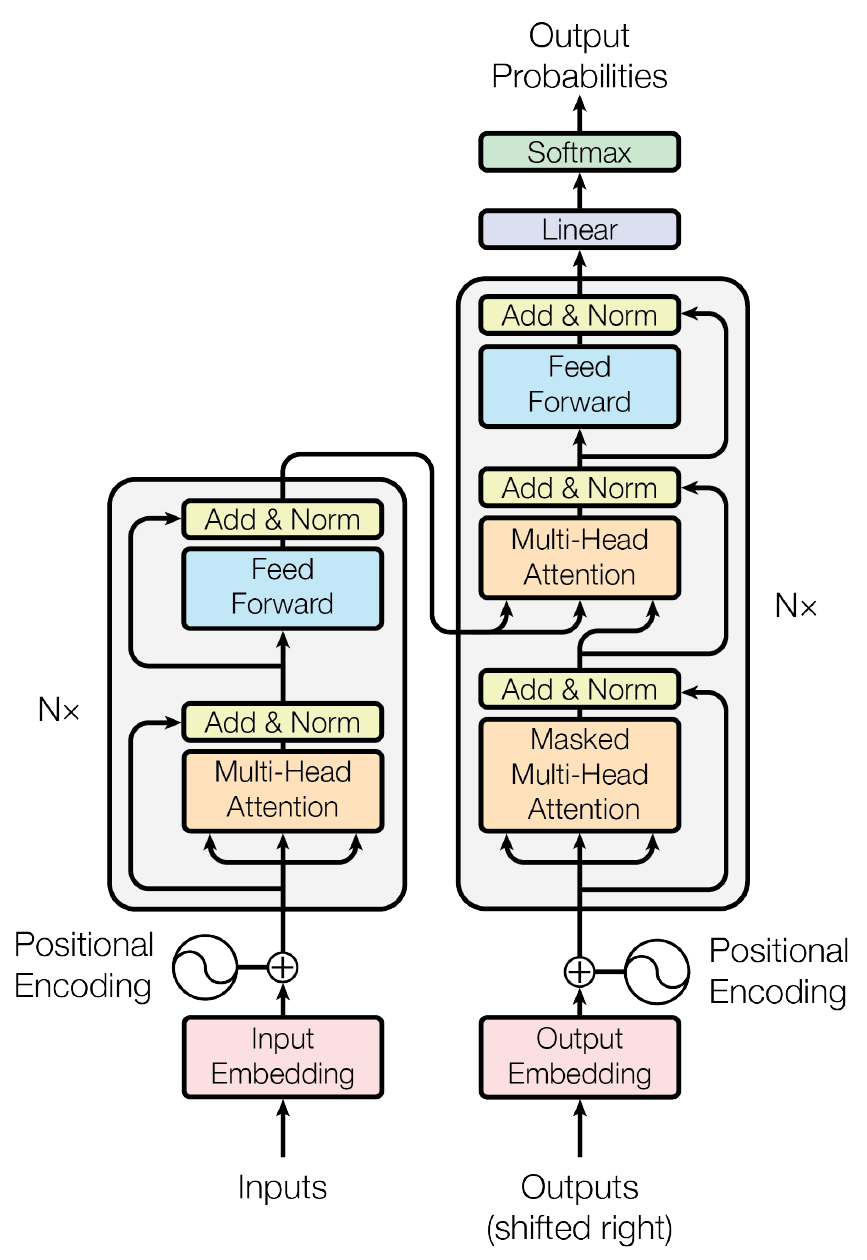
\includegraphics[width=0.8\textwidth]{zeichnungen/transformer.png}
    \caption[Die Transformer-Modell Architektur]{Die Transformer-Modell Architektur \citep{attention}}
    \label{bild:transformer}
\end{figure}

Die erste schriftliche Erwähnung des Transformer-Modells sowie die Einführung der beiden Teilmodelle Encoder und Decoder findet sich in \citet{attention}.
Die hier beschriebene bidirektionale Architektur bildet die Grundlage für alle darauf aufbauenden Modelle und Weiterentwicklungen.
Die Basisarchitektur wurde für verschiedene Anwendungen stark modifiziert.
Seit 2017 gibt es grundlegende Unterschiede in den Modellen und deren Möglichkeiten.
Aus diesem Grund haben \citet{ammus} eine Taxonomie der Transformer-basierten vortrainierten Sprachmodelle eingeführt.
Diese Taxonomie wird hier zur Beschreibung weiterer Architekturen und Methodiken verwendet.\\

Neben dem Grundbaustein eines Transformers --- dem Aufmerksamkeitsmechanismus --- sind zwei wichtige Modifikationen gegenüber normalen neuronalen Netzen in Transformer eingeflossen: Residuale Verbindungen und Dropout.\\

\subsubsection{Residuale Verbindungen}

\begin{definition}\label{def:residuale-verbindungen}
    \textbf{Residuale Verbindungen} oder auch Deep Residual Connections, sind direkte Verbindungen zwischen Eingabe und Ausgabe und überspringen somit eine oder mehrere Schichten eines \ac{nn}.
\end{definition}
Residuale Verbindungen als Level-Normalisierung ändern das Ziel eines \ac{nn}s, behalten aber die gleichen Ausgaben durch ihre Level-Normalisierung bei.
Dieses Konzept wurde erstmals in \citet{deep_residual} eingeführt und bietet eine Lösung für ein grundlegendes Problem von großen, mehrschichtigen Transformer-Modellen.
Bereits 2016 wurde im Bereich der Bilderkennung festgestellt, dass sich die Korrektheit von Modellen mit zunehmender Tiefe sättigt und sich dann rapide verschlechtert, wenn dieses Modell weiter trainiert wird.
Dies setzte eine praktische Grenze für die Tiefe von \ac{nn}s und verhinderte somit die Lösung komplexerer Probleme mit größeren Modellen.
\citet{deep_residual} beschreiben eine Lösung durch die genannten Residuen, die normale \ac{nn} einfach ersetzen können, und zeigen auch die Effizienz dieser Methode.\\

\subsubsection{Dropout}

Die Einführung von Dropouts ist die zweite wichtige Änderung zur Weiterentwicklung der Transformer-Architektur.
\begin{definition}\label{def:dropout}
    \textbf{Dropout} ist eine Methode, die die Trainingszeit von \ac{nn}s verkürzt und die Generalisierung verbessert.
    \citet{dropout} beschreiben die Methode als das zufällige Aussetzen von Neuronen unabhängig von der Eingabe in einem \ac{nn} während des Trainings.
\end{definition}
Durch das Aussetzen von Neuronen wird das \ac{nn} gezwungen, sich nicht auf andere Neuronen zu verlassen und somit eine bessere Generalisierung zu erreichen.
Das Aussetzen erfolgt nur während des Trainings und nicht während der Inferenz.
Die Methode wurde 2014 eingeführt und ist seitdem ein fester Bestandteil von \ac{nn}s.\\

\subsubsection{Modellarten von Transformer-Modellen}

Basierend auf der eingeführten Transformer-Architektur wurden verschiedene Modelltypen entwickelt, die nur Teile der Architektur nutzen und sich in ihrer Funktionsweise unterscheiden.

\begin{definition}\label{def:encoder-basierte-modelle}
    \textbf{Encoder-basierte Modelle} sind Sprachmodelle, die hauptsächlich auf der Encoder-Architektur basieren.
    Sie wurden entwickelt, um Eingabesequenzen zu verarbeiten und eine kompakte Repräsentation (auch Kontextvektor genannt) zu erzeugen.
\end{definition}
Die zentrale Komponente eines Encoder-basierten Modells ist der Encoder.
Er empfängt die Eingabesequenz und lernt schrittweise, die strukturellen und semantischen Informationen zu erfassen.
Die so erzeugte Repräsentation des Encoders kann von anderen Modulen oder Schichten des Modells verwendet werden, um verschiedene Aufgaben
wie z.B. die Klassifikation zu lösen.
Encoder-basierte Modelle haben in der Regel keine Decoder-Schicht.\\

\begin{definition}\label{def:decoder-basierte-modelle}
    \textbf{Decoder-basierte Modelle} sind Sprachmodelle, die auf einer speziellen Architektur basieren, bei der der Decoder eine zentrale Rolle spielt.
    Der Decoder ist eine Komponente, die darauf spezialisiert ist, aus einer gegebenen Eingabe eine sinnvolle und kohärente Ausgabe zu erzeugen.
\end{definition}
Im Zusammenhang mit der Textgenerierung erhält der Decoder normalerweise eine Sequenz von Vektoren als Eingabe, die von einem Encoder-Modul erzeugt wurde.
Bei der Textgenerierung kann der Decoder aus einer gegebenen Ausgangssequenz fortlaufend neue Wörter oder Sätze generieren, um einen zusammenhängenden Text zu erzeugen.

\subsection{Transformer-spezifische Architekturen}

\begin{definition}\label{def:self-attention-mechanismus}
    Der \textbf{Self-Attention-Mechanismus} ist ein zentrales Konzept in der Transformer-Architektur und beschreibt die Gewichtung der Eingabesequenz auf Basis eines aktuellen Tokens.
\end{definition}
Hier wird ein Eingabevektor in drei separate Vektoren transformiert:
Den Abfragevektor (engl. Query), den Schlüsselvektor (engl. Key) und den Wertvektor (engl. Value).
Anschließend wird die Ähnlichkeit zwischen dem Abfragevektor und dem Schlüsselvektor berechnet,
um die Aufmerksamkeitsgewichte zu erhalten.
Die Aufmerksamkeitsgewichte geben an, wie wichtig jeder Wertvektor für die Berechnung eines gewichteten
Durchschnitts ist. Die gewichteten Wertvektoren werden schließlich summiert, um den Ausgabevektor zu erhalten.

Die Self-Attention Mechanismen ermöglichen es den Modellen, komplexe Abhängigkeiten zwischen den Elementen einer Eingabesequenz zu erfassen.\\

\begin{definition}\label{def:multi-head-attention}
    \textbf{Multi-Head Attention} beschreibt den Ersatz eines einzelnen Self-Attention-Mechanismus in der Transformer-Architektur durch mehrere parallel arbeitende Self-Attention-Mechanismen.
\end{definition}
Beim Multi-Head Attention-Verfahren werden die Anfrage, der Schlüssel und der Wert $h$-mal linear auf mehrere Versionen projiziert und parallel berechnet. Die Ausgabe wird dann verkettet und erneut linear projiziert, um den Ausgabevektor zu erhalten. Multi-Head Attention ermöglicht es dem Modell, verschiedene Repräsentationsteilräume der Eingabe an verschiedenen Positionen zu erfassen.

\begin{definition}\label{def:feed-forward-netz}
    Ein \textbf{Feed-Forward-Netz} ist eine Art künstliches neuronales Netz, das aus mehreren Schichten besteht und Informationen nur vorwärts von der Eingabe zur Ausgabe fließen lässt.
\end{definition}
Feed-Forward-Netze haben keine zyklischen Verbindungen oder Rückkopplungsschleifen.
Sie dienen in Transformern neben den Aufmerksamkeitsnetzen als einzige zweite Komponente der Architektur.
Sie enthalten das erlernte Faktenwissen des Modells durch sogenannte Wissensneuronen \citep{knowledge_neurons}.\\

\subsection{Eigenheiten von Transformer-Modellen}
\begin{definition}\label{def:zeroshot-oneshot-multishot}
    Die Bezeichnungen \textbf{ZeroShot, OneShot} und \textbf{MultiShot} beziehen sich auf die Inferenz von Modellen.
    Die Eingabe enthält hier Beispielaufgaben, bevor die eigentliche Aufgabe gestellt wird.
\end{definition}
Insbesondere bei \ac{qa}-Aufgaben und Textgenerierungen werden diese Methoden häufig verwendet.
Bei der Beantwortung von Fragen können die Eingaben mehrere Beispielfragen und deren Antworten enthalten, bevor die eigentliche Frage gestellt wird.
Dadurch kann das Modell die Formatierung und Art der Aufgabe aus dem Kontext erkennen und bessere Antworten liefern.
\mbox{ZeroShot} bedeutet, dass das Modell keine Trainingsbeispiele erhält, um eine bestimmte Aufgabe zu lösen.
OneShot bedeutet, dass das Modell nur ein Trainingsbeispiel erhält, um eine bestimmte Aufgabe zu lösen.
MultiShot bedeutet, dass das Modell mehrere Trainingsbeispiele erhält.


\begin{definition}\label{def:parameterformate}
    \textbf{Parameterformate} sind Variableneinheiten von lernbaren Parametern.
    Häufig verwendet werden \enquote{Float16} und \enquote{Float32}.
\end{definition}
Sprachmodelle enthalten eine große Anzahl lernbarer Parameter (wie z.B. Gewichte und Bias),
sowie Zwischenwerte, die während der Inferenz berechnet werden.
Diese Werte können in unterschiedlichen Formaten gespeichert werden.
Gängige Formate sind hier \enquote{Float16} und \enquote{Float32}.
Float steht hier für Floating Value und stellt eine Fließkommazahl dar.
Die Zahl hinter Float gibt die Anzahl der Bits an, die zur Darstellung der Zahl verwendet werden.
Eine höhere Anzahl von Bits bedeutet eine höhere Genauigkeit und Wertebereich, aber auch einen höheren Speicherbedarf.

\begin{definition}\label{def:continual-pretraining}
    \textbf{Continual Pretraining} beschreibt den Prozess des kontinuierlichen, selbstüberwachten Trainings eines vortrainierten Modells.
\end{definition}
Beim Continual Pretraining werden nur die Hyperparameter des Modells angepasst und neue Datensätze verwendet, während auf die bereits erlernten Parameter des Modells aufbauend weitertrainiert wird.

%************ Transformer-Spezifische Eingaben

\subsection{Eingaben von Transformer-Modellen}
\begin{definition}\label{def:token}
    Ein \textbf{Token} repräsentiert eine Teilmenge eines Wortes und wird in Transformer-Modellen verwendet, um die Eingabe in logische Einheiten zu unterteilen.
\end{definition}
Transformer-Modelle können Eingaben nicht ohne zusätzliche Umwandlung verarbeiten.
Neben der Erzeugung von Eingabevektoren muss die Eingabe zunächst in kleinere Einheiten, so genannte Tokens, zerlegt werden.
Verschiedene ältere Modelle verwenden dazu Wörter oder Symbolunterteilungen.
Dies ist jedoch problematisch.\\

Durch die Zerlegung der Eingaben in Symbole ist zwar das Vokabular kleiner, welches zu schnelleren Trainingsdurchläufen führt, jedoch muss das Modell vor dem Erlernen von Wortzusammenhängen, Satzstrukturen und Sachverhalten zunächst die Bedeutung der Wörter und deren Zusammensetzung aus Symbolen erlernen.
Dadurch geht ein großer Teil der Trainingszeit für das Erlernen der Sprache verloren, was die endgültige Leistungsfähigkeit der Modelle stark einschränkt \citep{bpe}.\\

\begin{definition}\label{def:vokabular}
    Das \textbf{Vokabular} eines Modells ist die Menge aller Token, die das Modell als individuelle Einheiten erkennt. Die Größe des Vokabulars bestimmt die Größe der Input-Embeddings und begrenzt somit die Größe der Eingaben.
\end{definition}

Eine logische Schlussfolgerung wäre hier die Verwendung von Wörtern oder sogar Phrasen als Tokens.
Mit zunehmender Größe der Datensätze, die zum Training der Modelle verwendet werden, wächst das Vokabular enorm an.
Dies führt zu einer starken Verlangsamung der Trainingsläufe und zu sehr großen Modellen ohne Leistungsvorteil.
Wörter mit gleichem Wortstamm oder ähnlicher Bedeutung aufgrund grammatikalischer Regeln (Plural, Genus, Tempus) müssen vom Modell zunächst als \enquote{gleiches Wort} gelernt werden.
Daher hat sich die Unterteilung von Wörtern in Teilwörter als Standard durchgesetzt.

\subsubsection{Byte Pair Encoding}
\begin{definition}\label{def:bpe}
    \textbf{Byte Pair Encoding} ist ein Algorithmus, der iterativ ein Vokabular basierend auf der Häufigkeit von Symbolkombinationen in einem Datensatz aufbaut.
    Die Vokabulargröße ist der einzige Parameter.
\end{definition}
\citet{bpe} schlugen zu diesem Zweck die Verwendung von \ac{bpe} vor.
Die Unterteilung von Wörtern in Untergruppen von Wörtern hat bereits zu erheblichen Verbesserungen bei der Übersetzung von Sätzen geführt.
Sie hat sich aber auch in anderen Bereichen und Aufgaben wie der Textgenerierung, der Textklassifikation und der Analyse von Emotionen durchgesetzt.
Die Unterteilung von Wörtern ist hier eher als das Zusammensetzen von kleinen Teilwörtern zu verstehen.
Ausgehend von einem Vokabular, das aus allen Symbolen eines Alphabets besteht, wird dieses durch Zusammenfügen (engl. \enquote{Merge}) der Symbole erweitert, deren Kombination im Datensatz am häufigsten vorkommt.
Dieser Vorgang wird so lange wiederholt, bis die gewünschte Anzahl von Teilwörtern erreicht ist.
Die Anzahl der Teilwörter ist ein Hyperparameter, der je nach Modell und Datensatz variiert.\\

Die Unterteilung von Wörtern in Teilwörter hat den Vorteil, dass die Größe des Vokabulars nicht mit der Größe des Datensatzes wächst.
Dies führt zu einer schnelleren Eingabeverarbeitung und einer besseren Generalisierung der Modelle.
Die Unterteilung von Wörtern in Teilwörter hat jedoch auch Nachteile.
Sie ist nicht eindeutig, d.h. ein Wort kann in verschiedene Mengen von Teilwörtern zerlegt werden.
Dies führt zu einer größeren Anzahl möglicher Eingaben, die das Modell lernen muss.\\

Ein weiterer Nachteil ist, dass die Zerlegung von Wörtern in Teilwörter nicht immer sinnvoll ist.
So kann es vorkommen, dass ein Wort in Teilwörter zerlegt wird, die in der Sprache nicht existieren.
Dies wiederum minimiert die Verallgemeinerbarkeit der Modelle.
Ein Beispiel hierfür ist das Wort \enquote{Datensatz}.
Eine sinnvolle Unterteilung wäre hier \enquote{Daten} und \enquote{satz}, aber durch den Aufbau des Vokabulars aus den Symbolen des Datensatzes kann es vorkommen, dass das Teilwort \enquote{Daten} nicht die notwendige Häufigkeit besitzt und somit nicht im Vokabular vorhanden ist.
Daher muss auch dieses Wort zerlegt werden, z.B. in \enquote{Dat} und \enquote{en}.
Beide Teilwörter haben in der deutschen Sprache keine Bedeutung, werden aber durch das Modell mit Bedeutung versehen und in Beziehung zu anderen Wörtern gesetzt.
Dies führt zu einer unverständlichen Bedeutungsannotation von Teilwörtern und verschlechtert sowohl die Leistung als auch die Nachvollziehbarkeit des Modells und erschwert die Forschung an den Modellen.

\subsubsection{Eingabevektoren}

\begin{definition}\label{def:input-embeddings}
    \textbf{Input Embeddings} sind eine Darstellung der Eingabedaten in Form von Token in einem dichten Vektorraum.
\end{definition}
Die Repräsentation von Token in einem Vektorraum muss erlernt werden und ermöglicht es,
Token, die semantische Ähnlichkeiten oder Beziehungen zueinander aufweisen, geometrisch nahe beieinander zu platzieren.
Dadurch ist nicht nur das Token selbst, sondern auch die Beziehung zu anderen Tokens bekannt. Mit zunehmender Größe des Vokabulars müssen auch die Dimensionen der Input Embeddings vergrößert werden, da es sonst zu ungewollten Kollisionen zwischen Tokens kommen kann.

\begin{definition}[Positional Encodings]\label{def:positional-encodings}
    \textbf{Positional Encodings} stellen sogenannte relative und absolute Positionen der Token in der Eingabe dar.
\end{definition}
Relative und absolute Positionen von Token innerhalb einer Eingabe werden in einem Vektorraum dargestellt und ermöglichen es dem Modell, die Positionen der Token zu berücksichtigen.
Positional Encodings können gelernt oder berechnet werden und werden nur in Kombination mit Input Embeddings verwendet.

\section{Neuronale Netze}\label{sec:neuronale-netze}
Um die Architektur des Transformers zu verstehen, ist es notwendig, die Grundlagen neuronaler Netze zu kennen.
Neuronale Netze wurden erstmals 1943 von \citet{neuronal_networks_first} beschrieben und haben seitdem viele Veränderungen und Verbesserungen erfahren.
Eine Beschreibung der grundlegenden Techniken findet sich in \citet{neuronale-netze}.
Aufbauend auf diesem Buch wird im Folgenden ein Überblick über die Funktionsweise von Neuronalen Netzen gegeben.\\

\subsection{Architektur}
Neuronale Netze ahmen die Funktionsweise des menschlichen Gehirns mit Hilfe mathematischer Gleichungen nach.
Ein Netz besteht aus einer Anzahl von Neuronen, die sowohl Eingangs- als auch Ausgangsverbindungen zu anderen Neuronen haben.
Neuronen haben die Eigenschaft, von bestimmten Eingängen einen Impuls an die Ausgänge zu senden, wenn ein Schwellenwert überschritten wird.
Im Gegensatz zum Gehirn sind normale neuronale Netze jedoch logischer aufgebaut.
Die Neuronen sind in Schichten angeordnet, wobei die erste Schicht die Eingangsschicht mit den Eingangsneuronen $E_N$ und die letzte Schicht die Ausgangsschicht mit den Ausgangsneuronen $A_N$ ist.
Die Schichten zwischen diesen beiden Grenzen werden als versteckte Schichten (engl. \enquote{Hidden Layers}) mit Neuronen $H^L_N$ bezeichnet.\\

\begin{figure}
    \centering
    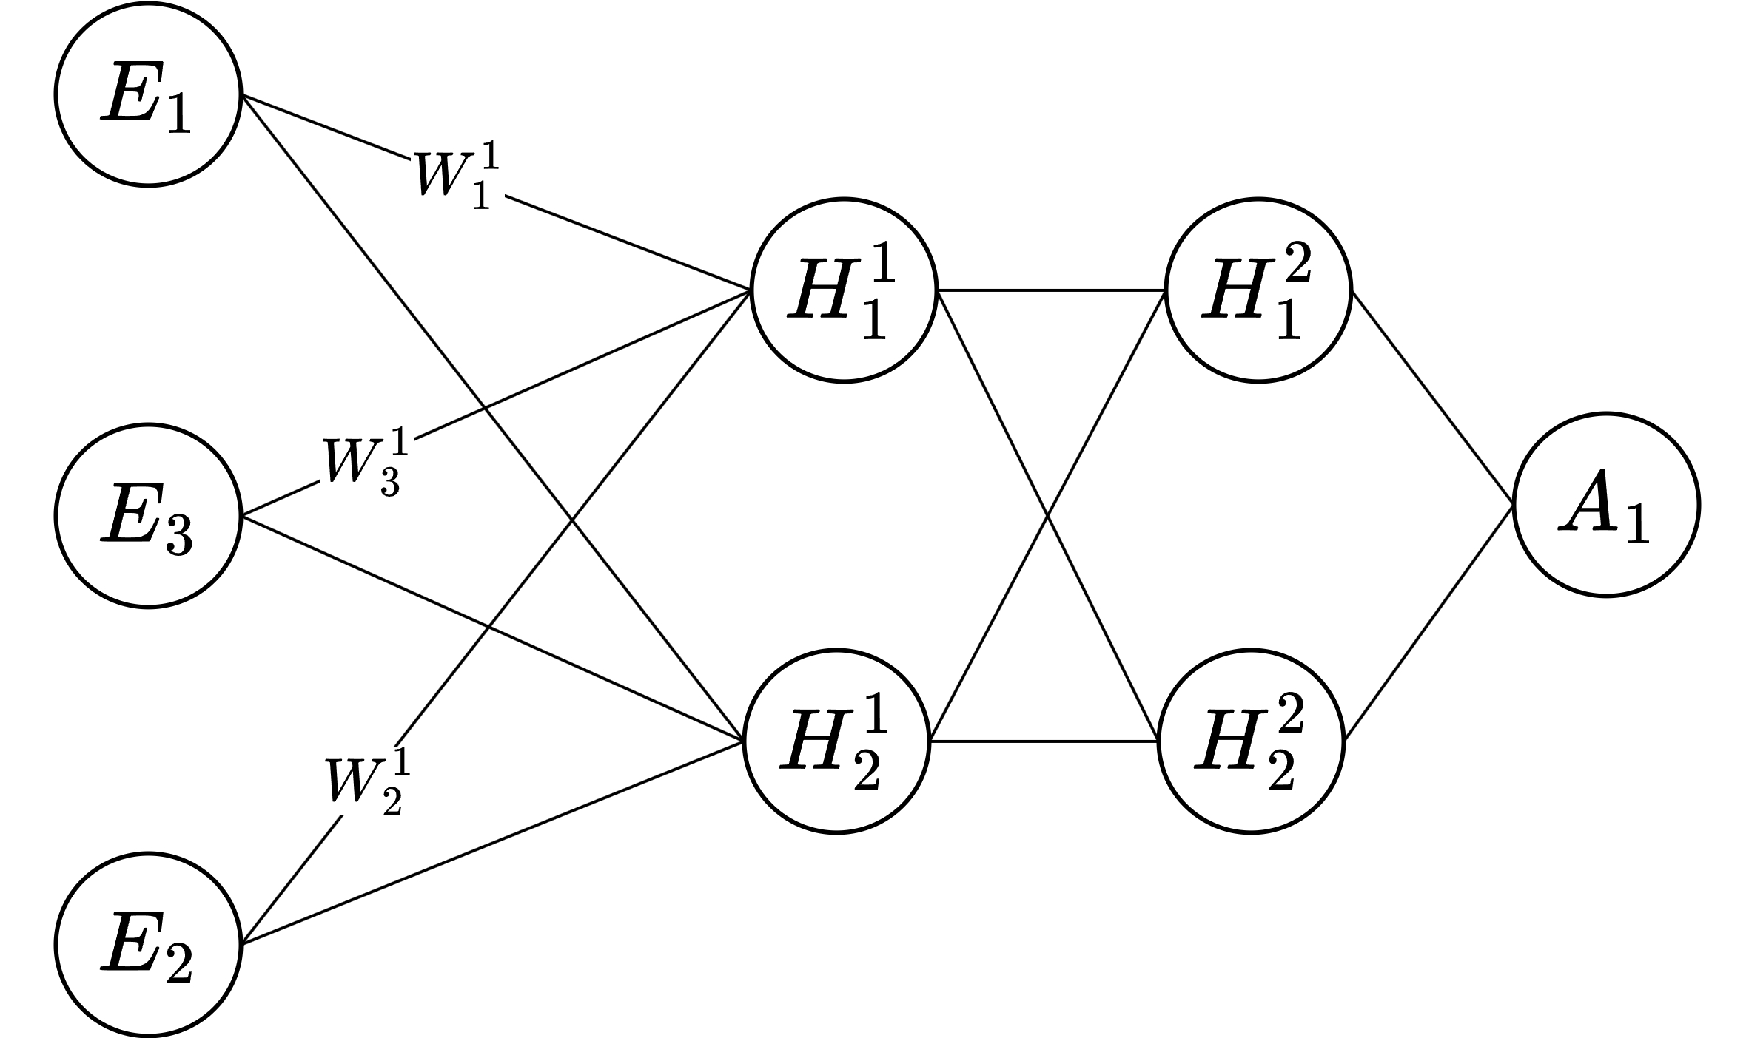
\includegraphics[width=\textwidth]{zeichnungen/nn_black.pdf}
    \caption[Beispiel-Aufbau eines Neuronalen Netzes]{Beispiel-Aufbau eines Neuronalen Netzes mit 3 Eingangsneuronen, 4 versteckten Neuronen und einem Ausgangsneuronen.}\label{nn_simple}
\end{figure}

\cref{nn_simple} zeigt eine Beispielkonfiguration mit 3 $E_N$, hier bezeichnet als $E_1,E_2,E_3$, zwei versteckten Schichten mit je zwei $H^L_N$, hier bezeichnet als $H^1_1, H^1_2$ und $H^2_1, H^2_2$ und einem Ausgangsneuron $A_1$.
Die Neuronen sind mit sogenannten Gewichten $W_N$ verbunden. Man spricht hier von einer Vorwärtsverbindung.
Das bedeutet, dass die Eingaben durch die Schichten in Richtung Ausgabe weitergereicht werden, aber nicht zurück zur Eingabe fließen können.
Im Beispiel in \cref{nn_simple} sind diese Verbindungen vollständig.
Jedes Neuron einer Schicht hat eine Verbindung zu jedem Neuron der nächsten Schicht.
Hier nicht gezeigt, hat jedes Neuron auch eine Eingangsverbindung von einem Bias $B_N$.

\subsection{Funktionsweise}
Die Anwendung des Neuronalen Netzes erfolgt in zwei Schritten.
Zuerst wird eine Eingabe in die Eingangsneuronen $E_N$ eingegeben.
Diese Eingabe wird durch die Schichten weitergegeben, bis sie in der Ausgabeschicht $A_N$ ankommt.
Jetzt muss das Ergebnis interpretiert werden. Dieser Vorgang wird auch als Inferenz bezeichnet.\\\
\begin{definition}\label{def:inferenz}
    \textbf{Inferenz} beschreibt den Prozess, bei dem ein Modell aufgrund der gelernten Parameter eine Vorhersage trifft.
\end{definition}

Ein Anwendungsbeispiel wäre die Erkennung von handgeschriebenen Zahlen.
Die Eingabe wäre hier ein Bild der Ziffer, das in ein neuronales Netz eingespeist wird.
Jedes Neuron repräsentiert den Grauwert eines Pixels im Bereich $[0;1]$.
Die Ausgabe stellt die erkannte Ziffer dar.
Für jede mögliche Ziffer (0-9) gibt es ein Ausgangsneuron, das vom neuronalen Netz einen Wert zwischen 0 und 1 erhält.
Das Neuron mit dem höchsten Ausgang repräsentiert die erkannte Ziffer.\\

Ein Berechnungsbeispiel für das erste Neuron der ersten versteckten Schicht $H^1_1$ sieht wie folgt aus:
\begin{equation}
    H^1_1=ReLU(W^1_1\cdot E_1 + W^1_2\cdot E_2 + W^1_3\cdot E_3 + B^1_1)
\end{equation}
$W^1_N$ stellen hier die Gewichte der ersten Schicht dar.
Gewichte sind Parameter, die während des Trainings eines Netzes angepasst werden, um eine optimale Ausgabe von $A_N$ zu erhalten.
Diese Parameter werden auch als lernbare Parameter bezeichnet.\\

\begin{definition}\label{def:lernbare-parameter}
    Ein \textbf{Lernbarer Parameter} ist ein Parameter, der zufällig initialisiert wird und während des Trainings angepasst wird.
\end{definition}

$B^1_N$ ist der Bias und ebenfalls ein lernbarer Parameter.
Alle Eingabewerte werden gemäß der Formel aufsummiert und mit Hilfe einer Aktivierungsfunktion transformiert.
Diese Aktivierungsfunktion war in früheren Netzen die Sigmoidfunktion \pcref{img:sigmoid}.
In modernen Netzen und auch in Transformer-Modellen wird hier die ReLU-Funktion \pcref{img:relu} verwendet.

\begin{figure}
    \centering
    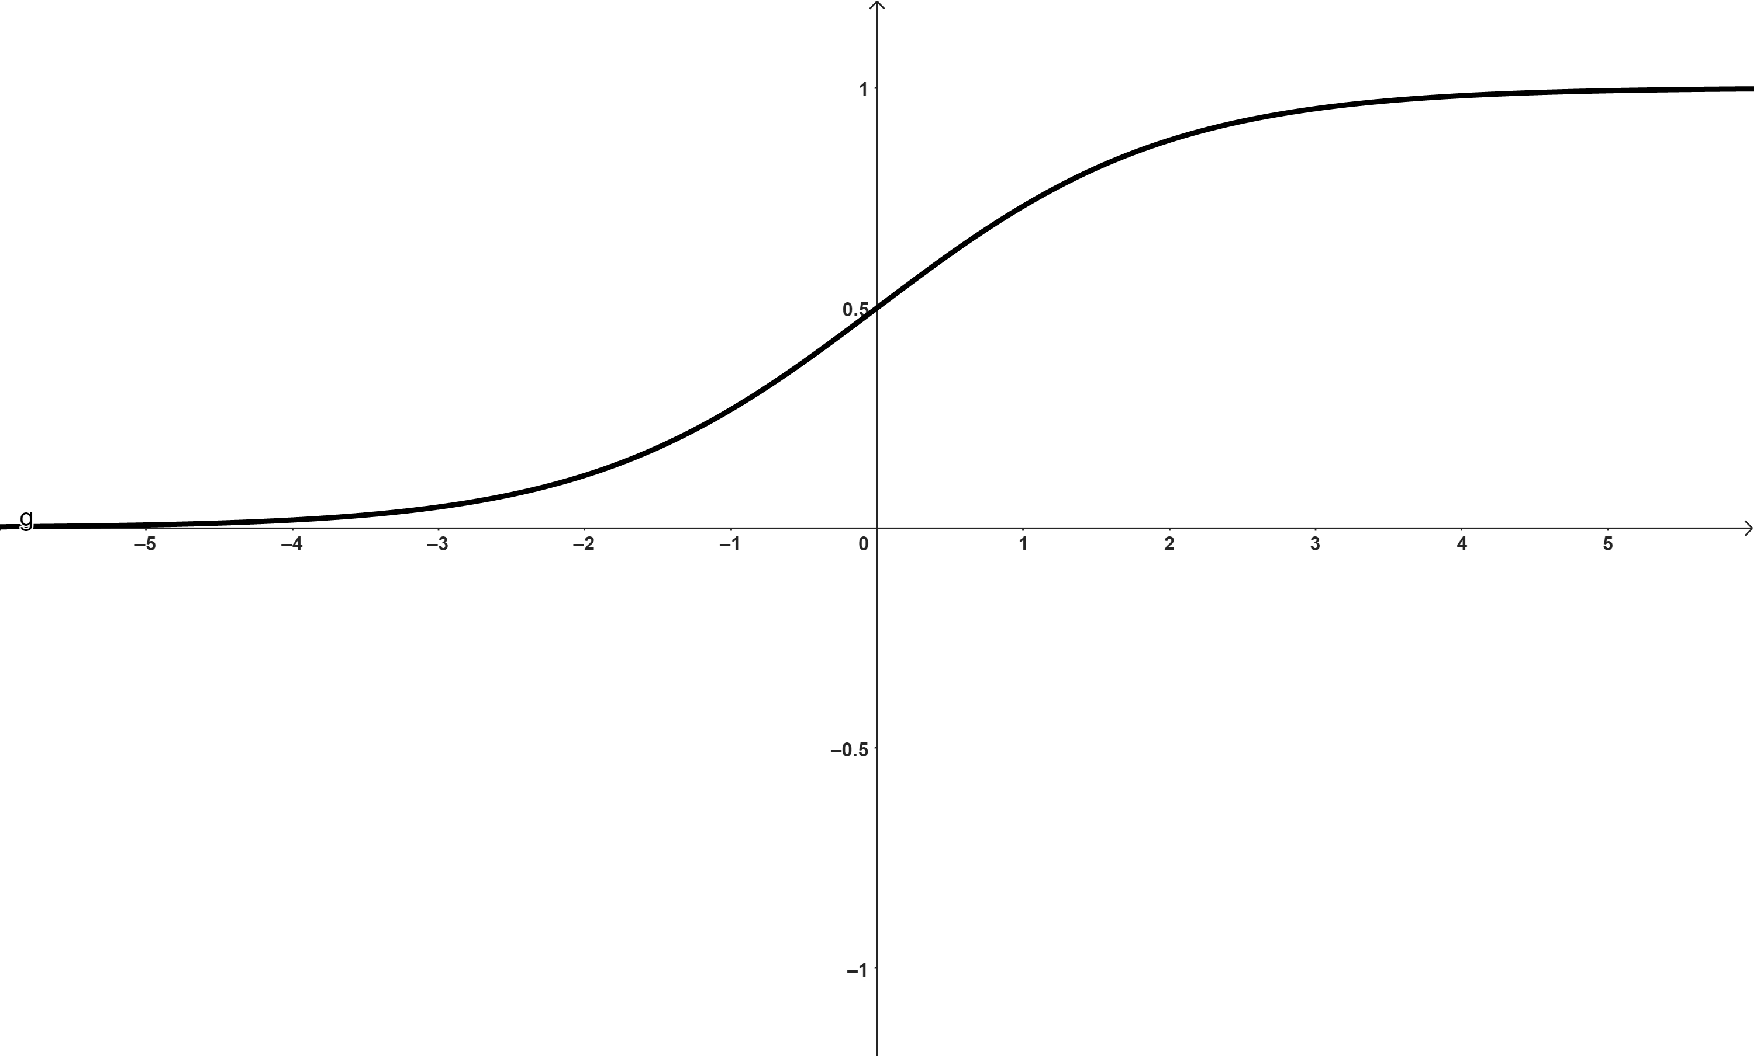
\includegraphics[width=0.8\textwidth]{zeichnungen/sigmoid_black.pdf}
    \caption[Die Sigmoid-Funktion]{Die Sigmoid-Funktion $f(x) = \frac{1}{1+e^{-x}}$}\label{img:sigmoid}
\end{figure}

\begin{figure}
    \centering
    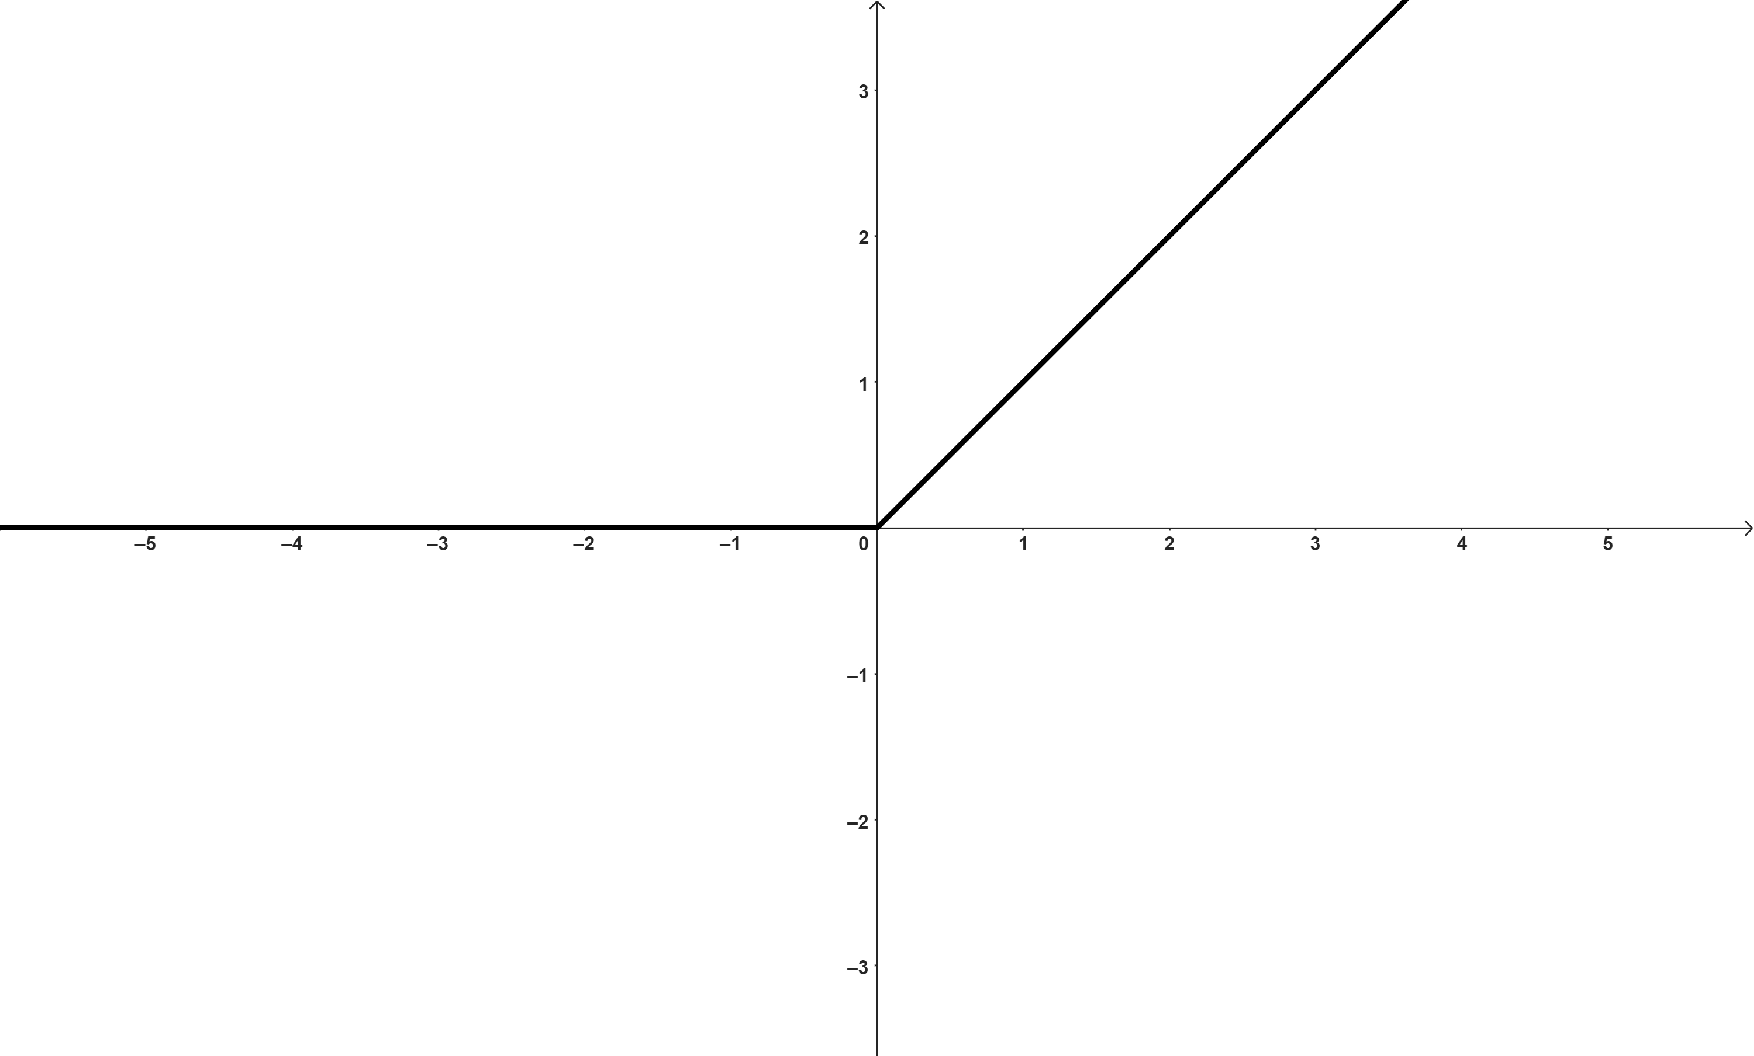
\includegraphics[width=0.8\textwidth]{zeichnungen/relu_black.pdf}
    \caption[Die ReLU-Funktion]{Die ReLU-Funktion $f(x) = \max(0,x)$}\label{img:relu}
\end{figure}

\begin{definition}\label{def:aktivierungsfunktion}
    Die \textbf{Aktivierungsfunktion} weißt jedem potentiellen Wert eines Neurons einen Wert in einem vorgegebenem Intervall zu.
    Sie ist nicht-linear und verhindert somit die Reduzierung eines Neuronalen Netzes auf eine lineare Funktion.
\end{definition}

Üblicherweise stellt eine Aktivierungsfunktion eine Transformation der Eingabewerte in einen nichtlinearen Ausgabewert zwischen 0 und 1 dar.
Dies ist jedoch nicht zwingend, da z.B. die ReLU-Funktion Werte zwischen 0 und $\infty$ ausgibt, aber schneller berechnet werden kann als die Sigmoidfunktion.
Aktivierungsfunktionen sind notwendig, um die Komplexität eines neuronalen Netzes zu erhöhen und damit seine Fähigkeit, komplexere Probleme zu lösen, zu ermöglichen.
Ohne Aktivierungsfunktion würden $A_N$ Neuronen eine Linearkombination der Eingabewerte erzeugen, wodurch nur lineare Probleme gelöst werden könnten.
Ein einfaches Beispiel ist die Berechnung der XOR-Funktion.
Die XOR-Funktion verknüpft zwei Eingaben zu einer Ausgabe. Wenn eine der beiden Eingaben 1 ist, soll auch die Ausgabe 1 sein.
Andernfalls soll die Ausgabe 0 sein.
Diese einfache Funktion kann ohne eine Aktivierungsfunktion nicht gelöst werden.\\

Die Ausgabewerte $A_N$ sind ebenfalls Werte im Bereich der Aktivierungsfunktion und nicht immer repräsentativ für das Problem, das das neuronale Netz lösen soll.
Daher werden diese Werte interpretiert und stellen häufig einen Konfidenzwert für eine bestimmte Klasse dar.
Wenn das Neuron $A_1$ den Maximalwert 1 hat, dann ist sich das Netz zu \SI{100}{\percent} sicher, dass die Eingabe der Klasse 1 entspricht.
Bei Transformern ist die Ausgabe $A_N$ ein Vektor über das gesamte Vokabular des Transformers und gibt an, inwieweit das Modell davon ausgeht, dass das jeweilige Token dem Eingabetext folgt.\\

\subsection{Training}\label{subsec:grundlagen:training}
Bevor ein neuronales Netz korrekte Ergebnisse liefern kann, muss es trainiert werden.
Training bedeutet die iterative Anpassung der Trainingsparameter, um eine möglichst gute Ausgabe zu erhalten.
Eine gute Ausgabe wird durch eine Fehlerfunktion beschrieben.
Diese Fehlerfunktion gibt einen einzelnen Wert zurück, der den Eingaben in das neuronale Netz entspricht und umgekehrt proportional zur guten Ausgabe ist.
Geometrisch stellt eine Fehlerfunktion eine mehrdimensionale Fläche dar, wobei jeder lernbare Parameter auf einer Achse liegt und das Minimum dieser Fläche ein Optimum darstellt.
Dieses Optimum ist das Trainingsziel.
Kleine Änderungen einzelner Parameter verändern die Ausgabe der Fehlerfunktion und können somit zeigen, ob diese Änderung zu einer Verbesserung oder Verschlechterung des neuronalen Netzes geführt hat.
Hier besteht bereits die Unterscheidung zwischen einem überwachten, selbstüberwachten und unüberwachten Lernverfahren.\\

\begin{definition}\label{def:ueberwachtes-lernen}
    Bei dem \textbf{Überwachten Lernen} sind sowohl die Eingabe als auch die erwartete Ausgabe während des Trainings bekannt.
    Die verwendete Fehlerfunktion ergibt sich aus der Differenz zwischen erwarteter und tatsächlicher Ausgabe.
\end{definition}

\begin{definition}\label{def:unueberwachtes-lernen}
    Bei dem \textbf{Unüberwachten Lernen} ist während des Trainings nur die Eingabe bekannt.
    Die Fehlerfunktion muss aus dem Kontext berechnet oder abgeleitet werden.
\end{definition}

\begin{definition}\label{def:selbstueberwachtes-lernen}
    Bei dem \textbf{selbstüberwachten Lernen} ist während des Trainings nur die Eingabe bekannt.
    Die Ausgabe entspricht jedoch einem Teil der Eingabe, so dass die Fehlerfunktion berechnet werden kann.
\end{definition}

Ein Beispiel für überwachtes Lernen ist die Klassifizierung von Bildern.
Der Datensatz enthält sowohl die Bilder als auch die zugehörigen Klassen.
Daher ist die erwartete Ausgabe des Modells für ein Bild genau die Klasse.
Transformer-Modelle sind selbstüberwachende Systeme.
Hier ergibt die Eingabe die erwartete Ausgabe, da das folgende Token der Eingabe als korrekt angesehen wird.
Unüberwachte Systeme sind z.B. Agenten, die Spiele lernen.
Hier gibt es in den meisten Fällen eine Belohnungsfunktion, die angibt, wie gut das Modell gespielt hat.
Belohnungsfunktionen können beschreiben, wie weit das Auto im Spiel gefahren ist oder wie viele Punkte gesammelt wurden.\\
\subsubsection{Backpropagation}\label{subsec:backpropagation}
\begin{definition}\label{def:backpropagation}
    \textbf{Backpropagation} beschreibt den Prozess der iterativen Anpassung von Gewichten und Bias auf Basis des Gradienten einer Fehlerfunktion.
\end{definition}

Eine der wichtigsten Methoden zur iterativen Anpassung von Gewichten und Bias und damit zum Training neuronaler Netze ist die Methode der Fehlerrückführung (engl. Backpropagation).
Diese Gradientenabstiegsmethode wurde erstmals 1986 von \citet{backpropagation} beschrieben und ist ausführlich in \citet{neuronale-netze} erklärt.
Um den Rahmen dieser Arbeit nicht zu sprengen, wird hier auf eine mathematische Beschreibung verzichtet und nur die Grundidee beschrieben.\\

Die Fehlerfunktion $C$ ist eine Funktion aller Gewichte und Bias des neuronalen Netzes und seiner Ausgabe.
Ihr Minimum zu finden bedeutet, ein Optimum für das Modell zu finden.
Zu Beginn des Trainings werden alle Gewichte mit Zufallszahlen initialisiert.
Nun wird die Ausgabe des Modells berechnet und mit der erwarteten Ausgabe verglichen.
Die Funktion $C$ hat einen Gradienten $\Delta C$, der die Richtung des steilsten Anstiegs der Funktion beschreibt.
Soll die Funktion minimiert werden, so wird der Gradient in die entgegengesetzte Richtung angewendet.
Dieser Gradient setzt sich aus partiellen Ableitungen der Fehlerfunktion über alle lernbaren Parameter zusammen.\\

\paragraph{Lernrate}
\begin{definition}\label{def:lernrate}
    Die \textbf{Lernrate} entspricht der Schrittweite des Gradientenabstiegs. Höhere Lernraten führen zu schnelleren Lernprozessen, können aber auch zu Oszillationen führen.
    Kleinere Lernraten führen zu langsameren Lernvorgängen und konvergieren möglicherweise nicht zu einem Minimum.
\end{definition}
Der Prozess des \enquote{Voranschreiten zum Minimum} bedeutet die Anpassung der lernbaren Parameter gemäß den partiellen Ableitungen.
Die Anpassung der Parameter ist ein Hyperparameter des Trainings und wird als Lernrate (engl. \enquote{Learning Rate}) bezeichnet.\\

\begin{definition}\label{def:hyperparameter}
    \textbf{Hyperparameter} sind Parameter, die Eigenschaften oder Techniken des Modells repräsentieren und vor dem Training festgelegt werden.
    Sie können vom neuronalen Netz nicht gelernt werden.
\end{definition}

Wird die Lernrate zu hoch gewählt, besteht die Gefahr, dass ein Minimum der Fehlerfunktion übersprungen wird und um diesen Punkt oszilliert.
Wählt man die Lernrate zu niedrig, so dauert das Training des neuronalen Netzes zu lange, um das Minimum zu erreichen.
Bei Transformern und tiefen neuronalen Netzen ist die Lernrate nicht konstant, sondern wird während des Trainingsprozesses regelmäßig angepasst.
Sehr große Modelle haben oft mehrere Milliarden Parameter und benötigen daher eine sehr kleine Lernrate, um nicht zu oszillieren.
Zu Beginn eines Trainings passt sich das Modell mit einer höheren Lernrate zu stark an kleine Änderungen an und findet ein lokales Minimum, das weit über dem globalen Minimum liegt.
Daher wird eine Aufwärmphase verwendet, um die Lernrate langsam zu erhöhen und das Modell an die Daten anzupassen.\\

Nach der Aufwärmphase wird die Lernrate langsam reduziert, so dass zu Beginn große Anpassungen der Parameter möglich sind und gegen Ende des Trainings nur noch eine Feinanpassung des gefundenen Minimums möglich ist.\\

\paragraph{Stochastischer Gradientenabstieg}\mbox{}\\
Die Berechnung des Gradienten der Fehlerfunktion über alle lernbaren Parameter ist nur sinnvoll, wenn sie über den gesamten Datensatz berechnet wird.
Jede Eingabe des Datensatzes verändert die Ausgabe des Modells und somit auch die Fehlerfunktion.
Das arithmetische Mittel der Fehlerfunktionen über alle Eingaben des Datensatzes ist die Fehlerfunktion des gesamten Datensatzes.

\begin{equation}
    C = \frac{1}{n}\sum_{k=0}^{n-1}C_k\\
\end{equation}

Hierbei ist $n$ die Anzahl der Eingaben des Datensatzes und $C_k$ die Fehlerfunktion der $k$-ten Eingabe.
Die Berechnung des Gradienten über alle Eingaben des Datensatzes ist jedoch sehr rechenintensiv und wird daher durch eine Stichprobe des Datensatzes ersetzt.
Diese Stichprobe wird als Batch bezeichnet.\\

\begin{definition}\label{def:batch}
    Ein \textbf{Batch} repräsentiert eine Teilmenge von Eingaben, welche geschlossen verarbeitet werden, bevor die Gewichte und Bias angepasst werden.
\end{definition}

Die Größe des Batches ist ein weiterer Hyperparameter des Trainings.
Die Berechnung des Gradienten über einen Batch wird als Stochastic Gradient Descent bezeichnet, da die Stichprobe des Datensatzes nur eine Approximation des Gradienten ist.
Dies bedeutet, dass die Richtung des Gradienten nur näherungsweise dem tatsächlichen Gradienten entspricht, die Berechnung aber wesentlich schneller ist.
Die Größe des Batches ist ein Kompromiss zwischen der Genauigkeit des Gradienten und der Geschwindigkeit der Berechnung.\\

\paragraph{Overfitting}
\begin{definition}\label{def:overfitting}
    \textbf{Overfitting} beschreibt den Prozess, bei dem ein Modell die Trainingsdaten auswendig lernt und nicht mehr in der Lage ist,
    neue Daten korrekt zu klassifizieren. Overfitting kann durch einen Leistungsabfall zwischen Trainings- und Testdaten erkannt werden.
\end{definition}

Ein logisches Ende des Trainings ist erreicht, wenn sich die Fehlerfunktion über einen bestimmten Zeitraum nicht mehr ändert und somit ein lokales Minimum gefunden wurde.
Dieses lokale Minimum ist jedoch nicht immer erwünscht.
Modelle, die den Datensatz auswendig lernen, erreichen einen sehr guten Wert für die Fehlerfunktion, der Prozess der Backpropagation wirkt unterstützend.
Diese Modelle sind jedoch nicht in der Lage, neue Daten korrekt zu klassifizieren und sind daher für die Praxis ungeeignet.
Dieser Prozess des Auswendiglernens wird als Overfitting bezeichnet.\\

Overfitting kann durch verschiedene Methoden verhindert werden.
Um Overfitting zu erkennen, wird der Datensatz in Trainings- und Testdaten aufgeteilt.
Es wird nur auf den Trainingsdaten trainiert und mit den Testdaten verglichen.
So kann festgestellt werden, wie gut das Modell auf Daten generalisiert, die es noch nicht gesehen hat.
Nähert sich die Fehlerfunktion bei den Testdaten einem Minimum, kann das Training beendet werden, da weitere Parameteranpassungen nur zu einem Auswendiglernen des Trainingsdatensatzes führen.\\


\section{Datenverarbeitung}\label{sec:datenverarbeitung}
Um ein Modell trainieren zu können, müssen die verwendeten Datensätze in eine für das Modell verständliche Form gebracht werden.
\begin{definition}\label{def:datenkuration}
    \textbf{Datenkuration} beschreibt den Prozess der Datenaufbereitung, um diese für die Verarbeitung durch ein Modell vorzubereiten.
\end{definition}
Die Datenkuration ist ein wichtiger Schritt dieser Arbeit und wird weiter in \cref{sec:datenkuration} genauer beschrieben.
Da Modelle nicht mit normalen Textdateien wie Word oder PDF umgehen können, müssen diese in eine für das Modell verständliche Form umgewandelt werden.

\subsection{Glossar der Daten}
In dieser Arbeit geht es hauptsächlich um Daten und die darin enthaltenen Informationen und das Wissen.
Zum besseren Verständnis dieser Unterscheidung folgt hier die Definition nach \citet{bb}.

\begin{definition}\label{def:wissen}
    \textbf{Wissen} sind generelle Informationen über Konzepte in einer bestimmten Domäne.
\end{definition}
Im Kontext dieser Arbeit stellt Wissen Informationen aus \citet{bb} dar.
Diese Informationen müssen von einem Modell gelernt werden, um das darin enthaltene Wissen zu reproduzieren.

\begin{definition}\label{def:information}
    \textbf{Informationen} sind spezifische Festlegungen über Entitäten wie zum Beispiel Fakten, Dinge, Personen, Prozesse, Ideen, Konzepte oder Ereignisse.
\end{definition}
Eine Information ist unabhängig von ihrer Darstellung und ist das grundlegende Ziel dieser Arbeit.
Informationen können unterschiedlich formuliert sein, aber den gleichen Informationsgehalt enthalten.
Daher wird, wie in \cref{sec:approach:questions} beschrieben, eine Antwort auf eine Frage, die die richtige Information enthält, unabhängig von ihrer Darstellung als richtig angesehen.

\begin{definition}\label{def:daten}
    \textbf{Daten} sind Informationen oder Wissen in einer strukturierten Form, die für die Verarbeitung, Kommunikation oder Interpretation von Menschen oder Maschinen geeignet sind.
\end{definition}
Die in dieser Arbeit verwendeten Daten sind Eingabedaten wie das Buch von \citet{bb} und die Fragen zu diesem Buch, Ausgabedaten aus dem trainierten Modell
als Antworten auf die Fragen und Daten, die im Modell enthalten sind, aber nicht in einer für Menschen verständlichen Form vorliegen.

%\addtocontents{toc}{\protect\clearpage} % <--- just debug stuff, ignore
%*****************************************
\chapter{Stand der Forschung}\label{ch:relatedWork}
%*****************************************
\section{Continual Pretraining und die Nutzung von Sprachmodellen}

Ein Tranformer-Modell als Wissensbasis ist in \citet{chatgpt_qas} verglichen mit verschiedenen \ac{sota}-Modellen. 
Sie zeigen eine deutliche Verbesserung der Robustheit gegenüber fehlerhafter Eingabe, Erklärbarkeit von Antworten und Fragenverständnis von komplexeren Fragen mit mehreren Fakten durch ChatGPT, zeigen allerdings Probleme in der Aktualität von Informationen, dem Wissen zu spezifischen Domänen und dem wohl wichtigsten, der korrekten Beantwortung von Fragen. 
Grund hierfür ist eine grundlegene Eigenschaft von \ac{gpt}-Modellen, keine Inkorperation von aktuellen Informationen. 
Das Trainieren von \ac{gpt}-Modellen ist ein aufwändiger Prozess und kann nicht bei jeder Inferenz (der Nutzung des Modells durch die Generierung von Text) durchgeführt werden. 
Desweiteren wurde ChatGPT jedoch ohne zusätzliches Continual Pretraining genutzt.
Eine Anpassung auf Domänen und Verbesserung der Korrektheit von Antworten steht somit noch aus.\\

\citet{improve_language} zeigen die Verbesserung der Leistung von Transformer-Modellen durch Generative Pretraining und eine weitere Steigerung dieser durch überwachtes Fine-Tuning.
Auch hier zeigt sich eine deutlicher Trend. Mit steigender Größe des Datensatzes, steigender Länge des Trainingprozesses und steigender Größe der Modelle verbessern sich die Ergebnisse von Modellen.\\

Diesen Trend belegen \citet{scaling_laws} und berechnen hier den Einfluss von verschiedenen Einflussgrößen auf die Gesamtleistung eines Modells. Durch die hier genutzen Einflussgrößen lässt sich eine Vorhersage der Leistung eines Modells treffen. 
Der Artikel endet mit einer Vermutung auf die theoretische maximale Leistung und damit maximale Größe von Transformer-Modellen.\\

Um diesen beschriebenen Skalierungsregeln zu folgen, jedoch die Trainigszeit und notwendige Datenmenge zu reduzieren, gibt es die Möglichkeit Continual Pretraining zu nutzen. 
\citet{dont_stop_pretraining} wendeten diese Methodik an und zeigten, dass Modelle immens davon profitieren, Domäne-spezifisches Wissen zu adaptieren und aus der großen Menge an grundlegenden Daten bessere korrekte Antworten in einer spezifischen Domäne zu generieren. 
Erstmals in \citet{biobert} genutzt um das Basismodell \ac{bert} auf die biomedizinische Domäne anzupassen, erweitern \citet{dont_stop_pretraining} diese Methode und zeigen die Anwendbarkeit auf verschiedene Domänen und Aufgaben. 
Das Continual Pretraining auf Aufgaben-Spezifische Daten verbessert die Leistung für spezifischen Aufgaben, während die Trainingszeit 60 mal kürzer ausfällt im Vergleich zu Continual Pretraining auf Domäne. 
Eine Verbindung beider Arten liefert hier die besten Ergebnisse.\\

Doch nicht nur Continual Pretraining verbessern die Ausgaben der Modelle, sondern auch das überwachtes Fine-Tuning. 
\citet{finetuning} beschreiben in ihrem Artikel die Effektivität von Reinforcement Learning als Fine-Tuning Methode um die Aufgaben der Weiterführung und Zusammenfassung von Texten zu lösen. 
Fine-Tuning benötigt jedoch gekennzeichnete Daten (engl. \enquote{labeled data}, Daten mit bekannten korrekten Ausgaben), welche in der Regel aufwändig zu Erstellen sind und nicht immer in der notwendigen Menge zur Verfügung stehen. 
In dieser Arbeit wird von einem Fine-Tuning durch die fehlende Verfügbarkeit von gekennzeichneten Daten abgesehen.\\
\section{Aktuelle Modelle und deren Nutzbarkeit}

Mit der Feststellung, dass die Leistung von Modellen mit steigender Größe, Trainigszeit und Daten steigt, wurden eine Reihe an Modellen entworfen, welche unterschiedlichste Architekturen, Anwendungsfälle und Leistungen besitzen.
Erstmalig einen Durchbruch in der Leistung von Transformer-Modellen erreichten \citet{gpt2} mit dem \ac{gpt}-2 Modell.
Sie zeigten im Vergleich zum ersten veröffentlichten \ac{gpt}-1 Model \citep{gpt1}, dass Sprachmodelle Aufgaben lösen können, ohne explizit überwacht zu werden.
Ebenso stellten sie fest, dass die Größe eines Modells, sei es hier die Anzahl an Parametern, die Größe des Datensatzes oder die Länge des Trainings, eine grundlegende Notwendigkeit für eine erfolgreiche ZeroShot Nutzung ist.
Schon hier erreichten sie ohne jegliche Architekturänderung im ZeroShot Setting erfolgreiche, \ac{sota} kompetitive Ergebnisse abhängig von den Aufgaben.\\

OpenAI gelang mit \ac{gpt}-3 einen Durchbruch in Popularität und beschrieben ihr Vorgehen in \citet{gpt3}.
In ihrem Artikel belegten sie die Leistungssteigerung durch größere Modelle und zeigten, dass diese Leistung ebenso ohne Fine-Tuning erreicht werden kann. 
Auch verglichen sie das Verhalten der Antworten abhängig von FewShot und ZeroShot Eingaben, wobei ersteres bessere Ergebnisse erzielten. 
Diese Erkenntnisse unterstützen die Annahme, dass auch ohne Fine-Tuning das in dieser Arbeit verwendete Modell gute Leistungen erreichen kann.\\

Weiterführend im Jahr 2023 veröffentlichte OpenAI \ac{gpt}-4 und stellten dieses in \citet{gpt4} vor. 
Neben den weit aus besseren Ergebnissen durch ein noch größeres Modell mit mehr Parametern gelang es ihnen, nun auch Bild-Daten als Eingabe zu verarbeiten. 
Dieser Artikel wiederum unterstreicht die Annahme, dass größere Modelle bessere Leistung bringen und ein besseres Verständnis der natürlichen Sprache besitzen.
Eine Nutzung dieses Modells, ebenso wie \ac{gpt}-3 ist nicht möglich, da diese Modelle zum aktuellen Zeitpunkt nicht veröffentlicht wurden.\\

In Kontrast zu den bisherigen Modellen veröffentlichten \citet{gpt_neox} \ac{gpt}-NeoX. 
Ein Modell, welches in seiner Größe und Leistung \ac{gpt}-3 ähnelt, jedoch auf der Architektur von \ac{gpt}-J\footnote{Ben Wang \url{https://github.com/kingoflolz/mesh-transformer-jax} (abgerufen am 3.6.2023)} basierend im Open-Source Rahmen veröffentlicht wurde. 
Sie zeigten, dass die meisten interessanten Fähigkeiten eines Modells erst ab eine bestimmen Anzahl an Parametern gezeigt werden.\\

Zuletzt veröffentlichte \citet{llama} die \ac{llama}-Modelle in unterschiedlicher Größe. 
Ein klarer Vorteil gegenüber anderen Modellen in ihrer Nutzbarkeit ist hier der Fokus auf längere Trainings-Zeit und einem größeren Datensatz gegenüber der Größe des Modells. 
Sie zeigten bessere Ergebnisse in fast allen Aufgabenbereichen gegenüber anderen Modellen wie \ac{gpt}-3 und \ac{palm} mit wesentlich weniger Parametern. 
Dadurch ist eine Nutzung jener Modelle billiger und schneller, einfacher und schneller zu trainieren mit gleichen oder besseren Ergebnissen. 
Auch diese Modelle wurden veröffentlicht und stehen somit zur Auswahl für diese Arbeit.

\section{Forschung und Probleme von Modellen}
Neben der Entwicklung von neuen Modellen wurden auch neue Ansätze zur besserem Continual Pretraining und Adaption von Modellen entworfen. 
\citet{adapterhub} stellten in ihrem Artikel die Adapter vor, welche ein Einsatz von zusätzlichen \ac{nn}s in verschiedene Ebenen der Transformer-Architektur ermöglichen.
Durch sie lässt sich die Adaption zu anderen Aufgaben und Domänen ohne Continual Pretraining des gesamten Modells erreichen, da während des Trainings sämtliche Parameter des Ursprungmodells fixiert bleiben, während die neu eingefügten Adapter trainiert werden.
Zusätzlich lassen sich dadurch bereits vortrainierte Adapter zu weiteren Domänen und Aufgaben in aktuelle Modelle einfügen, ohne die Notwendigkeit jeglichen Trainings.
Das veröffentliche System basiert auf dem Artikel von \citet{adapter_build_on}, in denen die Autoren das \ac{bert}-Modell auf 26 verschiedene \ac{nlp}-Aufgaben trainierten, mit einer Anpassung von nur 3,6\% Parametern und 0,4\% Leistungsminimierung (ein ursprüngliches Training der Modelle auf diese Aufgaben hätte 100\% aller Parameter angepasst). Sie bewiesen damit die Effizienz dieser Vorgehensweise, ohne eine große Beeinträchtigung der Ergebnisse.\\

\citet{knowledge_neurons} untersuchten die Fähigkeiten von \ac{llm}s auf ihre Eigenschaft, faktisches Wissen wiedergeben zu können, ohne eine Wissensdatenbank als Grundlage während der Nutzung zu besitzen.
Sie stellten fest, dass besonders in weiter hinten liegenden Ebenen die Neuronalen Netze sogenannte \enquote{Wissensneuronen} besitzen, die zu bestimmen Fakten korrelieren.
Diese Wissensneuronen aktiveren sich, wenn ein bestimmter Fakt in der Eingabe angesprochen wird und können mittels Verstärkung oder Unterdrückung dazu führen, dass das Modell diesen Fakt besser berücksichtigt oder \enquote{vergisst}.\\

Die Erforschung von Modellen und ihrer Eigenschaft Fakten zu erlernen und zu reproduzieren stoßen \citet{knowledge_base} an. Die hier verwendeten Modelle \ac{bert} und \ac{elmo} wurden auf ihr Potential als unüberwachtes Open-Domain \ac{qas} untersucht und zeigten gute Ergebnisse im Vergleich zu anderen \ac{sota}-Systemen.
Fortführend untersuchen \citet{xfactr} Multilinguale Modelle auf gleiche Eigenschaften, erhielten jedoch deutlich schlechtere Ergebnisse. Diese Ergebnisse deuten daraufhin, dass ein multilinguales Modell deutlich schlechter geeignet für die Nutzung als \ac{qas} ist, da ein Großteil der Leistung dieser Modelle in das Verständnis von Übersetzungen in andere Sprachen fließt.\\

Neben den überaus großen Erfolgen von neuen Modellen erheben sich jedoch auch neue Probleme bei der Benutzung dieser Modelle.
Neben Falschaussagen ergeben sich Probleme durch sozialen und anderen Bias in den Antworten, Selbstüberschätzung bei falschen Aussagen, welches wiederum zu schwerwiegenden Problemen in der Anwendung dieser Modelle kommen kann, Generierung von schädlichen Inhalten, Unterstützung von Kriminalität mit Expertise und weiteren Probleme. Eine Analyse der Ergebnisse dieser Arbeit im Bezug zu den ethischen Richtlinien der \ac{gmds} findet sich in \ref{sec:gmds_ethik}.
\citet{gpt4} dedizierten einen eigenen Abschnitt ihres Artikels zur Untersuchung dieser Probleme und deren Adressierung.
Sie zeigten hier grundlegende Probleme bei der Anwendung von Sprachmodellen auf, hielten jedoch konkreten Lösungsansätzen zurück.\\

In \citet{plagiarism} beschreibt der Autor weitere Fragestellungen zu dem Umgang mit Antworten von Sprachmodellen und deren Konflikt zum Urheberrecht.
Wem gehört der generierte Text - den Autoren der Datensätze auf dem das Modell trainiert wurde, der Firma dem das Modell gehört, dem Nutzer der das Modell anleitet? 
Auch hier zeigen sich ungelöste Probleme in der Anwendung von Sprachmodellen und bieten Raum für weitere Forschung. Eine definitive Antwort auf diese Fragen gibt es noch nicht, daher ist die Nutzung eines Sprachmodells zum Zeitpunkt dieser Arbeit nur abhängig von der Lizensierung des jeweiligen Modells durch die Autoren des Modells und der Lizensierung der Datensätze, die für das Continual Pretraining genutzt werden. Das hier verwendete Buch \citet{bb} steht unter der Open-Access Lizenz und kann somit uneingeschränkt für ein Continual Pretraining genutzt werden.\\

%*****************************************
\chapter{Lösungsansatz}\label{ch:approach}
%*****************************************
Diese Arbeit beschäftigt sich mit der Beantwortung von Wissensfragen zu \citet{bb} mit Hilfe
eines vortrainierten Sprachmodells, welches mit Hilfe des Buches \citet{bb} auf diese Domäne trainiert wird.
Die Aufgabenstellung unterteilt sich hier in fünf Teile:
\begin{enumerate}
    \item Die Auswahl eines Sprachmodells, welches die Aufgabe lösen kann.
    \item Die Kuration und Umwandlung des Buches von \citet{bb} in eine von dem Modell verständliche Form.
    \item Die Durchführung des Trainings des ausgewählten Modells.
    \item Die Erstellung eines Evaluierungsdatensatzes auf Basis von Klausuren, welche inhaltlich auf dem Buch von \citet{bb} basieren.
    \item Die Evaluierung des Modells mit Hilfe des erstellten Evaluierungsdatensatzes.
\end{enumerate}

\section{Auswahl von Sprachmodellen}
Für die Auswahl eines Sprachmodells müssen verschiedene Kriterien erfüllt sein.
Ausgehend von der Aufgabenstellung in \cref{sec:zielsetzung} stehen verschiedene Modelle der Transformer-Architektur zur Auswahl.
Die Auswahl beschränkt sich auf Decoder-basierte Modelle, da diese die Eigenschaften eines autoregressiven Modells besitzen.
Wie bereits in \cref{sec:grundlagen:transformer} beschrieben, ist das Ziel die Generierung von Text auf Basis einer Fragestellung. % TODO: Grundlagen Kapitel + Label
Diese Fragestellung wird zu Beginn als Eingabe zur Verfügung gestellt, woraufhin das Modell kontinuierlich neue Token generiert.
Neu generierte Token werden zusammen mit der ursprünglichen Frage als Eingabe verwendet, um den nächsten Token zu generieren.
Dieses Verhalten entspricht autoregressiven Modellen und erfordert Decoder-basierte Modelle.
Ein Decoder-basiertes Modell verwendet alle vorhergehenden Token, um Token zu generieren (auch als Vorhersage von Token bezeichnet), während ein Encoder-basiertes Modell sowohl vorhergehende als auch nachfolgende Token verwendet.
Encoder-basierte Modelle sind für die Textvervollständigung oder Textklassifikation gedacht, aber nicht für die Textgenerierung.\\

Zusätzlich sind folgende Eigenschaften erwünscht.
Das Modell soll eine gute ZeroShot-Performance haben und nicht nur eine gute FewShot- oder OneShot-Performance.
Diese Arbeit untersucht die Fähigkeit eines Modells, Wissen aus domänenspezifischer Literatur (hier aus \citet{bb}) zu reproduzieren.
Indem frühere Fragen und Antworten als Kontext verwendet werden, werden die Ergebnisse synthetisch durch zusätzliches Wissen im Kontext verbessert.
Einige Fragen könnten nicht durch das Modell mit Hilfe des gelernten Wissens beantwortet werden, sondern durch das Wissen im Kontext.
Das Modell soll auch ohne Fine-Tuning eine gute Leistung erbringen.
Da ein Fine-Tuning in dieser Arbeit aufgrund der fehlenden Datenmenge nicht möglich ist, soll ein Modell gewählt werden, das auch ohne dieses Fine-Tuning eine gute Performance erreicht.\\

\begin{table}
    \centering
    \setlength{\tabcolsep}{5pt}
    \resizebox{\textwidth}{!}{
    \begin{tabular}{lllll}
        \toprule
        Modell & Verfügbarkeit & ZeroShot & Größe & GPU-Speicher\\
        \midrule
        GPT-2       & frei               & schlecht  & 1,5 Mrd. Parameter & 24 GB\\
        GPT-3       & nur Interferenz   & gut       & 175 Mrd. Parameter & 1,4 TB\\
        GPT-4       & nur Interferenz   & sehr gut  & --- & --- \\
        GPT-J       & frei              & gut       & 6,7 Mrd. Parameter & 104 GB\\
        GPT-NeoX    & frei              & gut       & 20 Mrd. Parameter  & 160 GB\\
        \multirow{4}{*}{LLaMa}
                    & limitiert         & gut       & 7 Mrd. Parameter   & 56 GB\\
                    & limitiert         & gut       & 13 Mrd. Parameter  & 104 GB\\
                    & limitiert         & sehr gut  & 33 Mrd. Parameter  & 264 GB\\
                    & limitiert         & sehr gut  & 65 Mrd. Parameter  & 520 GB\\
        \bottomrule
    \end{tabular}}
    \caption{Übersicht über die zur Auswahl stehenden Modelle.\label{tab:approach:models}}
\end{table}

Die hier zur Auswahl stehenden Modelle sind GPT-2, GPT-3, GPT-4, GPT-J, GPT-NeoX und LLaMa, gezeigt in \cref{tab:approach:models}.
Die angegebenen GPU-Speicher Anforderungen beziehen sich hier auf die notwendige Speichermenge zum Training des Modells.
Berechnet wird diese mit der \cref{eq:speicher}.
\begin{equation}\label{eq:speicher}
    \text{Speicher}=\text{Anzahl Parameter} \cdot \frac{\text{Parameterformat}}{8} \cdot 4
\end{equation}
Verschiedene Modelle benutzen die Parameterformate FP16 oder FP32, welche 2 bzw. 4 Byte pro Parameter benötigen. Zusätzlich muss das Modell während des Trainings circa 4 mal in den Speicher geladen werden, um die Backpropagation durchzuführen. Zur Interferenz der Modelle ist dementsprechend ein Speicherbedarf von $\frac{1}{4}$ der angegebenen Werte notwendig.
Modelle, die sehr populär geworden sind, aber nicht zur Auswahl stehen, sind BERT, RoBERTa, DistillBERT, BART, T5, Opus, Pegasus, DialoGPT, Blenderbot und Flan-T5.
Wenn die Aufgabe des Question Answering gelöst werden soll, ist ein BERT-basiertes Modell die erste Wahl.\\

Modelle wie BERT, RoBERTa und DistillBERT besitzen aufgrund ihrer Encoder-Architektur optimale Eigenschaften für die Informationsextraktion aus Text.
Dieser Ansatz ist jedoch in zwei Punkten eingeschränkt.
Die Modelle lernen nicht Fakten und können auf Basis einer Frage neue Antworten formulieren, sondern finden Textstellen in einem Kontext, die die Frage beantworten.
Es findet keine Textgenerierung statt, sondern es werden Ausschnitte aus einem gegebenen Textkontext als Antwort gefunden.
Dieser Kontext ist wiederum durch die Größe des Modells begrenzt und beschränkt sich in den meisten Fällen auf 512 Token.
Ist die Antwort auf die Frage nicht im Kontext enthalten, kann das Modell keine Antwort finden.
Da die Fragen unabhängig vom Kontext beantwortet werden sollen, können diese Modelle nicht verwendet werden.
Andere Modelle wie BART, T5, Opus, Pegasus, DialoGPT, Blenderbot und Flan-T5 wurden für andere Aufgaben entwickelt und können nicht auf die vorliegende Aufgabe angewendet werden.
Sie sind für Textklassifikation, Textübersetzung, Textzusammenfassung, Dialoge oder Text-2-Text-Aufgaben konzipiert.\\

GPT-2 ist das kleinste Modell der OpenAI GPT-Serie und wurde erstmals in \citet{gpt2} vorgestellt.
Aufgrund seiner geringen Größe kann das Modell auf einzelnen \ac{gpu}s trainiert und verwendet (inferiert) werden, was die Nutzung des Modells erheblich vereinfacht.
Außerdem ist es frei verfügbar und kann ohne weitere Maßnahmen verwendet werden.
Allerdings ist die Performance in der Einstellung ZeroShot nicht ausreichend.
Das Modell erreicht eine Imitation von Texten, aber kein Verständnis und keine Wiedergabe von Fakten.

GPT-3 und das darauf basierende GPT-3.5 (ChatGPT), vorgestellt in \citet{gpt3}, ist zum Zeitpunkt der Arbeit frei nutzbar, hat eine sehr gute ZeroShot-Performance und ist groß genug, um als QA-Modell zu dienen.
Das Modell ist jedoch nicht frei verfügbar.
Es existiert zwar eine \ac{api}, diese dient jedoch nur zur Interferenz des Modells, ein Training ist nicht möglich.
Damit scheidet das Modell bereits aus.
Ein weiteres Problem ist die Größe des Modells.
Bei ca. 175 Milliarden Parametern ist eine Nutzung des Modells erst mit 8 A100 \ac{gpu}s möglich.
Das Training benötigt zusätzlich etwa die 4-fache Leistung.
Diese Leistung kann zwar vom Rechenzentrum der Universität Leipzig zur Verfügung gestellt werden, verhindert aber den Einsatz des Modells in einer längerfristigen Umgebung.\\

GPT-4 ist das mächtigste Modell von OpenAI und wurde in \citet{gpt4} vorgestellt.
Auch dieses Modell ist nicht frei verfügbar und kann nur über eine \ac{api} verwendet werden.
Die Leistungsfähigkeit von GPT-4 ist jedoch deutlich höher als die von GPT-3, weshalb die Untersuchung dieses Modells als Ersatz für ein speziell trainiertes Modell geplant ist.
Die Größe des Modells wurde von OpenAI nicht veröffentlicht, ist aber definitiv größer als GPT-3, weshalb eine Verwendung hier allein aufgrund der Größe ausscheidet.\\

GPT-J erreicht mit 6,7 Milliarden Parametern die Größe des kleinsten Modells der GPT-3 Serie, zeigt aber eine deutlich bessere Performance als GPT-2.
Das Modell ist unter \citet{gptj} veröffentlicht und frei verfügbar.
Die Leistungsfähigkeit des Modells ist im Vergleich zu den anderen Modellen in der Auswahl geringer und wird daher ausgeschlossen.\\

GPT-NeoX wurde in \citet{gpt_neox} vorgestellt und erreicht mit einer Größe von 20 Milliarden Parametern die Leistungsfähigkeit von GPT-3 mit 175 Milliarden Parametern.
Das Modell ist frei verfügbar und kann ohne weitere Maßnahmen verwendet werden.
Die Leistung des Modells ist vergleichbar mit GPT-3, während die Größe des Modells ein Training mit 8 A100 \ac{gpu}s erlaubt.
Diese Leistung wird jedoch von LLaMa übertroffen und daher nicht ausgewählt.\\

Die in \citet{llama} vorgestellten LLaMa-Modelle haben einen besonderen Ansatz.
Durch den Fokus auf längeres Training und größere Datensätze bieten sie parametereffiziente Modelle, die sehr gute Leistungen erzielen können.
Die Modelle von LLaMa werden ausgewählt, um die bestmögliche Performance mit den kleinstmöglichen Modellen zu erreichen.
Hier stellt sich die Frage, welches Modell aus der LLaMa-Reihe verwendet werden soll.
Die Modelle unterscheiden sich sowohl in der Größe als auch proportional in der Leistung.\\

\begin{table}[t!]
    \centering
    \setlength{\tabcolsep}{5pt}
    \resizebox{\textwidth}{!}{
    \begin{tabular}{lrccccccccc}
    \toprule
    & & BoolQ & PIQA & SIQA & \hspace{-0.3cm} HellaSwag \hspace{-0.2cm} & \hspace{-0.2cm} WinoGrande \hspace{-0.3cm} & ARC-e & ARC-c & OBQA \\
    \midrule
    GPT-3        & 175B & 60.5 & 81.0 & -    & 78.9 & 70.2 & 68.8 & 51.4 & 57.6 \\
    Gopher       & 280B & 79.3 & 81.8 & 50.6 & 79.2 & 70.1 & -    & -    & -    \\
    Chinchilla   & 70B  & 83.7 & 81.8 & 51.3 & 80.8 & 74.9 & -    & -    & -    \\
    PaLM         & 62B  & 84.8 & 80.5 & -    & 79.7 & 77.0 & 75.2 & 52.5 & 50.4 \\
    PaLM-cont    & 62B  & 83.9 & 81.4 & -    & 80.6 & 77.0 & -    & -    & -    \\
    PaLM         & 540B & \textbf{88.0} & 82.3 & - & 83.4 & \textbf{81.1} & 76.6 & 53.0 & 53.4 \\
    \midrule
    \multirow{4}{*}{LLaMa}
       & 7B   & 76.5 & 79.8       & 48.9 & 76.1 & 70.1 & 72.8       & 47.6       & 57.2 \\
       & 13B  & 78.1 & 80.1       & 50.4 & 79.2 & 73.0 & 74.8       & 52.7       & 56.4 \\
       & 33B  & 83.1 & 82.3 & 50.4 & 82.8 & 76.0 & \textbf{80.0} & \textbf{57.8} & 58.6       \\
       & 65B  & 85.3 & \textbf{82.8}  & \textbf{52.3} &  \textbf{84.2}    &  77.0    & 78.9  & 56.0 &   \textbf{60.2} \\
  \bottomrule
    \end{tabular}}
\caption{
Zero-Shot Leistung verschiedener Modelle in Begründungsaufgaben für gesunden Menschenverstand.
Veröffentlicht in \citet{llama}\label{tab:llama_naturalquestion}
}
\end{table}

Die \cref{tab:llama_naturalquestion} zeigt die Leistungsfähigkeit der Modelle im Vergleich zu anderen Modellen und bei verschiedenen Einstellungen (ZeroShot bis 64Shot).
Selbst das kleinste Modell mit 7 Milliarden Parametern übertrifft die Leistung von GPT-3 und kann während der Interferenz auf einer einzelnen V100 \ac{gpu} verwendet werden.
Nach Angaben der Autoren kann auch das Modell mit 13 Milliarden Parametern auf einer einzigen V100 \ac{gpu} eingesetzt werden, was für die Wahl dieses Modells spricht.
Das 33-Milliarden-Parameter-Modell erzielt im ZeroShot sogar etwas bessere Ergebnisse als das 65-Milliarden-Parameter-Modell, weshalb die Wahl des 33-Milliarden-Parameter-Modells hier sinnvoll ist.
Mit 33 Milliarden Parametern und der Verwendung von Float16 Werten (auch Half-Precision genannt) benötigt das Modell 66 GB \ac{gpu} RAM, um für die Interferenz verwendet werden zu können.
Für das Training werden 264 GB \ac{gpu} RAM benötigt, was 4 A100 \ac{gpu}s entspricht.
Das Modell mit 65 Milliarden Parametern benötigt 7 A100 \ac{gpu}s für das Training und 2 A100 \ac{gpu}s für den Betrieb.
Aufgrund der vielversprechenden ZeroShot-Performance wird in dieser Arbeit das Modell mit 33 Milliarden Parametern gewählt.
Die Modelle sind jedoch nicht öffentlich verfügbar, sondern werden nur zu Forschungszwecken über einen Antrag veröffentlicht.
Dieser Antrag wurde im Rahmen dieser Arbeit gestellt und genehmigt.\\

Eine Alternative zu den LLaMa-Modellen ist OpenLLaMa, veröffentlicht unter \citet{openllama}.
Die hier verfügbaren Modelle mit 3 Milliarden, 7 Milliarden und 13 Milliarden Parametern entsprechen in ihrer Leistungsfähigkeit den LLaMa-Modellen, sind aber unter der Open-Source-Lizenz Apache 2.0 verfügbar.
Da jedoch kein Modell mit 33 Milliarden Parametern verfügbar ist, wird auf diese Modelle verzichtet.\\

In dieser Arbeit werden die Modelle LLaMa 7B und 33B verwendet, da sie eine sehr gute Leistung mit minimalen Ressourcenanforderungen bieten. Eine Auswahl beider Modellgrößen begründet sich daher, dass eine Nutzung des 33B Modells auf einzelnen GPUs nicht möglich ist, und dadurch die Nutzbarkeit eingeschränkt wird. Deshalb wird ebenso die Leistung des kleinsten LLaMa Modells zum Vergleich herangezogen.\\

\section{Datenkuration}
Um die Literatur optimal nutzen zu können, muss eine Datenkuration durchgeführt werden.
Die Daten liegen im Word-Format vor, können aber in diesem Format nicht verarbeitet werden, da das Modell nur Text verarbeiten kann.
Die Datenkuration umfasst mehrere Schritte, die im Folgenden beschrieben werden.\\

\subsection{Extraktion der Texte}
Die Extraktion der Text wird händisch durchgeführt.
Dazu wird das Word-Dokument geöffnet und der Text kopiert.
Der Text wird in einem Texteditor eingefügt und als \texttt{.md} Datei gespeichert.
\texttt{.md}-Dateien folgen dem Markdown-Format und haben die besondere Eigenschaft, mit Hilfe von Text-Symbolen Formatierungen wie Überschriften, Aufzählungen und Tabellen darzustellen.

\subsection{Unverständliche Formate}
Die Extraktion des Textes erfolgt manuell.
Dazu wird das Word-Dokument geöffnet und der Text kopiert.
Der Text wird in einen Texteditor eingefügt und als \texttt{.md}-Datei gespeichert.
\texttt{.md}-Dateien folgen dem Markdown-Format und haben die besondere Eigenschaft, Formatierungen wie Überschriften, Aufzählungen und Tabellen mit Hilfe von Textsymbolen darzustellen.

\subsection{Textpassagen ohne Wissen oder Kontext}
Teile des Dokuments enthalten kein Wissen, stehen in keinem Zusammenhang oder sind für das Modell unverständlich formatiert.
Die Titelseite wird auf den Buchtitel reduziert, das Vorwort wird weggelassen, da es kein Wissen zum Thema enthält, Tabellen- und Abbildungsverzeichnisse werden ebenfalls entfernt.
Bild- und Tabellenverzeichnisse enthalten zwar Wissen, können aber nicht in Kontext gesetzt werden, da die verwendeten Attention-Mechanismen des Modells diese Verzeichnisse nicht mit Texten in späteren Kapiteln verknüpfen können, da der Kontext zu groß ist.
Auch die Vorstellung der Autoren enthält kein Wissen zum Thema und wird daher entfernt.
Zusätzlich werden fehlerhafte Textpassagen wie fehlende Verweise entfernt.
Diese Textstellen existieren nur in der Word-Version des Buches, nicht aber in der endgültigen PDF-Version.
Da eine Textextraktion aus PDF-Dateien jedoch zu gravierenden Problemen in der Textformatierung führt, wurde darauf verzichtet.

\subsection{Optionale Textentfernungen}
Es soll geprüft werden, ob das Weglassen von Literaturverweisen, Überschriften und Tabellen zu einer besseren Leistung führt.
Literaturverzeichnisse beziehen sich auf das vorhergehende Kapitel, haben aber ein schwieriges Format.
Insbesondere \ac{url}s müssen vom Modell in Token zerlegt werden, die nicht den Inhalt der \ac{url}s widerspiegeln. 
Überschriften haben im Vergleich zum Text nur einen minimalen Anteil an der Gesamtzahl der Tokens, wodurch das in ihnen enthaltene Wissen verloren geht.
Die menschenlesbare Formatierung einer Überschrift hat keinen Einfluss auf die Bewertung durch das Modell.
Tabellen liegen in einem Format vor, das vom Modell nicht nativ verarbeitet werden kann.
Selbst die Tabellendarstellung in Markdown ist zwar einlesbar, aber es ist fraglich, ob sie verständlich ist.
Aufgrund der geringen Größe des Datensatzes ist auch nicht zu erwarten, dass dieses Format verstanden wird.
Daher wird hier eine Aufzählung als Tabellenersatz verwendet.

\subsection{Bleibende Texte}
Das Abkürzungsverzeichnis und das Glossar bleiben im Text enthalten, da sie für das Verständnis der Fragen wichtige Begriffe definieren.
Einige Fragen können Akronyme oder Fachbegriffe verwenden, die vom Modell verstanden werden müssen.

\subsection{Formatierung von Text}
Die Formatierung des Textes im Word-Dokument kann nicht berücksichtigt werden.
Daher muss hier ein Ersatz in Form einer Markdown-Formatierung gefunden werden.
Überschriften werden durch \texttt{\#}, Aufzählungen durch \texttt{-} und \texttt{1.} dargestellt.
Tabellen werden durch eine Aufzählung dargestellt, wobei die erste Zeile die Überschriften enthält und die zweite Zeile die Trennung zwischen Überschriften und Inhalt darstellt.
Die Trennung zwischen den Spalten erfolgt durch \texttt{|}.
Hoch- und tiefgestellte Zahlen werden durch \texttt{\^} und \texttt{\_} dargestellt.
Formeln werden im \LaTeX{} Mathe-Modus dargestellt.

\subsection{Potentielle Extraktion von Fragen}
Neben der Verwendung des Textes als Eingabe in das Modell ist auch eine weitergehende Nutzung möglich.
Die Übungsabschnitte sowie das Glossar und das Abkürzungsverzeichnis können als Quelle für Fragen genutzt werden,
um das Modell und andere Modelle besser bewerten zu können.

\section{Unüberwachtes Weitertrainieren}
Um das LLaMa-Modell zu trainieren, wird ein Programm benötigt, das den Datensatz in Token umwandelt und diese dann in Batches an das Modell übergibt.
Basierend auf diesen Batches wird das Modell verwendet, um die Gewichte mittels Backpropagation anzupassen.
Dieser Prozess stellt somit eine Epoche dar.
Bei kleineren Datensätzen und Fine-Tuning werden oft mehrere Epochen gewählt, während größere Datensätze (mehrere hundert Gigabyte) nur eine Epoche oder nicht einmal eine Epoche benötigen.
Mit zunehmender Epoche passt sich das Modell immer mehr an die Literatur an, bis eine Grenze überschritten wird.
Diese Grenze wird oft als \enquote{Overfitting} bezeichnet und stellt ein Modell dar, das sich zu sehr an einen Datensatz angepasst hat.
Dadurch verliert das Modell die Fähigkeit, auf unbekannte Daten zu verallgemeinern, was in diesem Anwendungsfall dazu führt, dass keine Fragen mehr beantwortet werden können.\\

Um Overfitting zu vermeiden, wird der Datensatz in einen Trainings- und einen Validierungsdatensatz aufgeteilt.
Dabei wird eine Aufteilung von \SI{90}{\percent} Training und \SI{10}{\percent} Validierung verwendet.
Das Modell wird nur auf dem Trainingsdatensatz trainiert, aber in regelmäßigen Abständen mit dem Validierungsdatensatz überprüft.
Die Ergebnisse des Validierungsdatensatzes haben keinen Einfluss auf die Anpassung der Gewichte, sondern dienen nur zur Überprüfung der Generalisierungsfähigkeit des Modells.
Sowohl für den Trainings- als auch für den Validierungsdatensatz wird ein Absinken der Kostenfunktion erwartet.
Dieses Absinken ist ein Indikator dafür, dass das Modell sich an den Datensatz anpasst.
Sobald das Absinken auf dem Validierungsdatensatz aufhört, ist das Training abgeschlossen.
Die Ergebnisse zeigen in den meisten Fällen, dass die Kostenfunktion des Trainingsdatensatzes niedriger ist als die des Validierungsdatensatzes.
Solange der Unterschied zwischen den beiden Kostenfunktionen nicht zu groß ist, konnte das Modell erfolgreich trainiert werden.\\

Für die Umsetzung dieser Trainingsschritte wird die Programmiersprache Python verwendet, da sie eine Vielzahl von Bibliotheken für die Textverarbeitung und den Einsatz von neuronalen Netzen bietet.
Die Bibliothek Transformers von HuggingFace bietet eine Vielzahl von Modellen und Trainingsmethoden und basiert auf der populären Bibliothek PyTorch.
PyTorch bietet mit Hilfe von CUDA die Möglichkeit, Trainingsschritte auf einer Nvidia \ac{gpu} durchzuführen, was die in \cref{sec:grundlagen:training} beschriebenen Rechenschritte um ein Vielfaches beschleunigt. % TODO: Rechenschritte in Grundlagen erklären, label hinzufügen
Mit Hilfe von DeepSpeed kann dieses Training auch auf mehrere \ac{gpu}s verteilt werden.
Dies ist notwendig, da das verwendete Modell mit 33 Milliarden Parametern zu groß ist, um in den Arbeitsspeicher einer einzelnen \ac{gpu} zu passen.\\

Vor Beginn des Trainings müssen einige Konfigurationsparameter festgelegt werden.
Diese Parameter sind in der \cref{tab:training:parameter} aufgelistet und folgen den Trainingsparametern von \citet{llama}.
\begin{table}
    \centering
    \begin{tabular}{ll}
        \toprule
        \textbf{Parameter} & \textbf{Wert} \\
        \midrule
        Lernrate & $1,5e^{-4}$\\
        AdamW $\beta_1$ & 0,9\\
        AdamW $\beta_2$ & 0,95\\
        Gewichtsreduktion & 0,1\\
        Gradientenlimitierung & 1,0\\
        Aufwärmphase & 0\\
        Epochen & 2\\
        \bottomrule
    \end{tabular}
    \caption{Parameter für das Training des LLaMa 33B-Modells}\label{tab:training:parameter}
\end{table}

Die Lernrate (engl. \enquote{Learning Rate}) ist ein Parameter, der das Ausmaß der Anpassung der Gewichte bestimmt.
Je höher die Lernrate, desto stärker werden die Gewichte angepasst.
Dies kann dazu führen, dass das Modell nicht konvergiert, sondern über den optimalen Punkt hinausschießt.
Bei einer zu niedrigen Lernrate konvergiert das Modell sehr langsam.
Die Lernrate wird während des Trainings angepasst, um eine schnelle Konvergenz zu ermöglichen.
Diese Anpassung folgt dem Kosinus-Lernratenschema, so dass die endgültige Lernrate \SI{10}{\percent} des Anfangswertes beträgt.
Die Lernraten hängen von der Modellgröße ab.
Im Allgemeinen benötigen größere Modelle eine niedrigere Lernrate.
Der Optimierer AdamW berücksichtigt den zeitlichen Abfall der Gewichte und wurde in \citet{adamw} vorgestellt.
Er ist die häufigste Wahl in aktuellen Modellen und wurde auch für das Training der LLaMa-Modelle verwendet.\\

Gewichtsabnahme (engl. \enquote{Weight Decay}) ist ein Parameter, der die Gewichte während des Trainings reduziert.
Er stellt eine Regularisierung dar, die Overfitting verhindern soll.
$0,1$ entspricht einer Gewichtsreduktion von \SI{10}{\percent}.\\

Die Gradientenbegrenzung (engl. \enquote{Gradient Clipping}) ist ein Parameter, der die Größe der Gradienten begrenzt.
Dies ist notwendig, da bei großen Modellen die Gradienten während der Backpropagation mit zunehmender Tiefe immer größer werden.
Ohne eine Begrenzung würden die Gradienten hier exponentiell wachsen.
Eine Gradientenbegrenzung beschränkt die Gradienten auf $1.0$\\

Die Aufwärmphase beschreibt die Anzahl der Schritte, die das Modell benötigt, um die Lernrate von $0$ linear auf den Anfangswert zu erhöhen.
Dies ist notwendig, da sich die Modelle zu Beginn des Trainings zu schnell an nicht universelle Muster anpassen.
Normalerweise wird dies durch ein längeres Training korrigiert, bei dem die zuerst gelernten Muster wieder verlernt werden müssen.
Durch die Aufwärmphase wird ein längeres Training vermieden.
Da in diesem Fall das Modell bereits auf einem großen Datensatz trainiert wurde, ist eine Aufwärmphase nicht notwendig.

Der Artikel von \citet{llama} beschreibt ein Training über eine Epoche.
Da in diesem Fall jedoch der Datensatz im Vergleich minimal ist, wird eine größere Anzahl von Epochen verwendet.\\

\subsection{Ausführen der Training-Programme}

Zur Ausführung der Trainingsprogramme wird SLURM\footnote{\url{https://slurm.schedmd.com/overview.html} (abgerufen am 16.6.2023)} verwendet.
Mit Hilfe von SLURM-Skripten können Programme über mehrere Knoten, \ac{cpu}s und \ac{gpu}s verteilt berechnet werden.
Diese Skriptsprache wird vom Rechenzentrum der Universität Leipzig verwendet, um verschiedene Programme auf den Supercomputern Clara und Paula laufen zu lassen.\\

Die Supercomputer Clara und Paula sind Rechennetze, die auf \ac{gpu}beschleunigte Berechnungen spezialisiert sind.
Paula besteht aus 12 Knoten mit je 8 Nvidia Tesla A30 \ac{gpu}s.
Clara ist zweigeteilt und besteht aus 8 Nodes mit je 4 Nvidia Tesla V100 \ac{gpu}s und 22 Nodes mit je 8 Nvidia GeForce RTX 2080 TI \ac{gpu}s.
Die Knoten sind über ein Infiniband-Netzwerk verbunden, das eine hohe Bandbreite und geringe Latenz bietet.\\

Supercomputer sind gemeinsam genutzte Ressourcen, die von mehreren Nutzern gebucht werden können.
Die Auswahl der Supercomputer hängt also davon ab, welche Knoten gerade frei sind.
Generell werden Clara-Nodes mit V100 \ac{gpu}s bevorzugt, da hier der größtmögliche Speicher pro \ac{gpu} zur Verfügung steht.
Dies hat zur Folge, dass weniger Knoten gleichzeitig reserviert werden müssen, was die Wartezeit verkürzt und die Kommunikation zwischen den Knoten minimiert.\\

Die Trainingsprogramme müssen auch in der Lage sein, mit der Multi-\ac{gpu}-Architektur umzugehen.
Dazu wird die Bibliothek DeepSpeed \citep{deepspeed} in Kombination mit der Bibliothek Transformers verwendet.
DeepSpeed erlaubt verschiedene Arten der Parallelisierung, der Fokus liegt hier auf ZeRO 2 \citep{ZeRO}.
Die ZeRO Parallelisierung erlaubt eine verteilte parallele Datenverarbeitung, bei der das Modell auf mehrere \ac{gpu}s aufgeteilt wird.
Ohne diese Option ist ein Training nicht möglich, da, wie oben beschrieben, einzelne Modelle nicht vollständig auf eine \ac{gpu} passen.
Genauere Erläuterungen zur Konfiguration von DeepSpeed und zur Verwendung der Transformer-Bibliothek sind in \cref{ch:solution} beschrieben.
% TODO: Kapitel Solutions reminder

\section{Klausurfragen}\label{sec:approach:questions}
Zur Überprüfung der Modelle werden Klausurfragen verwendet.
Diese Klausurfragen ergeben sich aus den mündlichen Prüfungsfragen des Moduls \enquote{Architektur von Informationssystemen im Gesundheitswesen},
den schriftlichen Prüfungsfragen des Moduls \enquote{Informationssysteme in medizinischer Versorgung und Forschung} und aus Teilen des Buches \citet{bb}.
Die Fragen sind in drei Kategorien unterteilt:
\begin{enumerate}
    \item Einzelfragen, die einen bestimmten Sachverhalt abfragen
    \item Multi-Fakten-Fragen, die mehrere Fakten abfragen
    \item Transferfragen, die einen Sachverhalt von einem Kontext in einen anderen übertragen
\end{enumerate}

Allerdings ist die Anzahl der durchgeführten Klausuren zum Zeitpunkt der Erstellung dieser Arbeit geringer als erwartet, da der Studiengang erst seit 2021 existiert.
Dies führt zu einer geringeren Qualität der Bewertung,
hat aber keinen Einfluss auf die Qualität des Modells.\\

Die LLaMa-Modelle sind ohne weiteres Fine-Tuning verfügbar und wurden daher nicht an die Aufgabe der Beantwortung von Fragen angepasst.
Dies hat zur Folge, dass die Modelle bei einer Frage wie \enquote{Welche Farbe hat der Himmel?} nicht die Antwort liefern, sondern den Text im gleichen Stil mit weiteren Fragen fortsetzen.
Um eine Antwort auf eine Frage zu erhalten, muss die Frage in eine unvollständige Aussage umformuliert werden.
Im gegebenen Beispiel wird aus \enquote{Welche Farbe hat der Himmel?} die Aussage \enquote{Der Himmel hat die Farbe}, die dann vom Modell mit \enquote{blau.} beantwortet wird.
Dieser Prozess der Umformulierung von Fragen wird für alle vorhandenen Fragen durchgeführt.
Das \ac{gpt}-4-Modell wurde auf die Aufgabe der Beantwortung von Fragen trainiert und kann daher mit normalen Fragen evaluiert werden.\\

Einige Fragen erfordern das Zeichnen von Systemen oder das Verbinden von Begriffen mit Pfeilen.
Da das Modell keine Bilder erzeugen kann, werden diese Fragen so umformuliert, dass sie als Textfragen beantwortet werden können.
Eine Skizze wird entsprechend in eine Systembeschreibung umformuliert und eine Begriffsverbindung in eine Begriffsliste.
Andere Fragen bauen auf Lösungen der vorhergehenden Frage auf.
Dies ist nur dann sinnvoll, wenn das Modell den Verlauf der Fragestellungen kennt, was nicht der Fall ist.
Diese Fragen müssen ebenfalls umformuliert werden, um unabhängig von anderen Fragen zu sein.

\section{Modellvergleich}
Der Vergleich der Modelle erfolgt im Rahmen einer manuellen Bewertung.
Dazu werden die in \cref{sec:approach:questions} definierten Fragen verwendet.
Diese Fragen werden von dem LLaMa Modell 7B und 33B sowohl vor als auch nach dem Continual Pretraining und von GPT-4 beantwortet.
Die Antworten werden manuell ausgewertet und mit den Antworten aus dem Buch \citet{bb} verglichen.
Die Lösungen werden ebenfalls in drei Kategorien eingeteilt:
\begin{enumerate}
    \item Richtig, wenn die Antwort mit der Antwort im Buch übereinstimmt
    \item Falsch, wenn die Antwort falsches Wissen enthält
    \item Nicht beantwortet, wenn der generierte Text keinen Bezug zur Frage hat
\end{enumerate}

Die Modelle werden mit Hilfe der micro-F1 Bewertung verglichen.
Die Definition folgt den unter \citet{chatgpt_qas} beschriebenen Formeln:
\begin{ceqn} % TODO: mprec und mrecall ausformulieren
\begin{align}
    C &= S \cap G \\
    m_{prec} &= \frac{\sum_{i=1}^{N}|C_{qi}|}{\sum_{i=1}^{N}|S_{qi}|} \\
    m_{recall} &= \frac{\sum_{i=1}^{N}|C_{qi}|}{\sum_{i=1}^{N}|G_{qi}|} \\
    microF1 &= \frac{2 \cdot m_{prec} \cdot m_{recall}}{m_{prec} + m_{recall}}
\end{align}
\end{ceqn}
% TODO: MacroF1 nutzen? oder begründen warum microF1
Dabei ist $S_q$ die Menge der für die Fragen $q$ generierten Antworten, $G_q$ die Menge der richtigen Antworten aus dem Buch \citet{bb} und $C_q$ die Menge der richtigen Antworten, die sowohl in $S_q$ als auch in $G_q$ enthalten sind.
$N$ ist die Anzahl der Fragen, $m_{prec}$ die Mikro-Präzision und $m_{recall}$ der Mikro-Recall.
Der Wert $microF1$ ist das harmonische Mittel aus $m_{prec}$ und $m_{recall}$.
Fragen gelten als beantwortet, wenn sie den Kategorien 1 und 2 entsprechen.
Dieselben Berechnungen werden insgesamt und getrennt für alle drei Fragekategorien durchgeführt.
Mikro-Präzision beschreibt den Anteil richtiger Antworten an allen beantworteten Fragen.
Der Mikro-Recall beschreibt den Anteil der richtigen Antworten an allen Fragen.\\

Den in \citet{chatgpt_qas} beschriebenen Ansatz folgend werden die Modelle auf die Kriterien Korrektheit, Determinismus, Robustheit, Erklärbarkeit und Fragenverständnis evaluiert.
Die Kriterien \enquote{Nutzung aktueller Informationen} und \enquote{Generalisierung über verschiedene Domänen} werden nicht betrachtet, da die Modelle keinen Zugriff auf aktuelle Informationen und verschiedene Domänen haben.\\

\noindent\textbf{Korrektheit:}\newline
Die Korrektheit wird durch die oben beschriebenen Formeln berechnet und verglichen.
Eine höhere Korrektheit entspricht einem besseren Ergebnis.
Bei der Anwendung des Modells ist eine hohe Mikro-Präzision wichtiger als ein hoher Mikro-Recall, da eine falsche Antwort für einen unkundigen Anwender wesentlich schädlicher ist als keine Antwort.
Die Modelle sollen immer keine Antwort einer falschen Antwort vorziehen.\\

\noindent\textbf{Determinismus:}\newline
Determinismus beschreibt die Reproduzierbarkeit von Antworten.
Für die gleiche Frage und das gleiche Modell sollen die Antworten immer gleich sein.
Sprachmodelle zeigen ein gewisses Maß an nichtdeterministischem Verhalten, daher ist diese Statisik ein wichtiges Kriterium.
Um dies zu erreichen, werden Fragen 3 mal an die Modelle gestellt und die beste Antwort wird zur Berechnung der Korrektheit verwendet.
Dabei wird auch diese Statistik berechnet.
Eine Antwort gilt als deterministisch, wenn die gleichen Fakten mit leichten Umformulierungen in der Antwort enthalten sind.\\

\noindent\textbf{Robustheit:}\newline
Die Robustheit beschreibt die Fähigkeit des Modells, auch bei fehlerhaften Eingaben korrekte Antworten zu generieren.
Dazu werden grammatikalische Fehler sowie Rechtschreibfehler in eine Teilmenge der Fragen eingefügt und die Korrektheit der Antworten berechnet.
Eine Antwort wird als robust bezeichnet, wenn sie auch bei fehlerhaften Eingaben korrekt ist.\\

\noindent\textbf{Erklärbarkeit:}\newline
Die Erklärbarkeit beschreibt die Fähigkeit des Modells, die erzeugten Antworten zu erklären.
Dazu werden die Modellantworten manuell daraufhin überprüft, ob sie eine Erklärung enthalten.
Ist dies nicht der Fall, wird eine zusätzliche Eingabe erzeugt, der nach einer Erklärung fragt.
Eine Antwort gilt als erklärbar, wenn sie eine Erklärung enthält.
Die Ergebnisse werden in \enquote{ohne zusätzliche Eingabe} und \enquote{mit zusätzlicher Eingabe} unterschieden.\\

\noindent\textbf{Fragenverständnis:}\newline
Das Fragenverständnis beschreibt die Fähigkeit des Modells, die Frage zu verstehen.
Dazu werden die Antworten der Modelle manuell daraufhin überprüft, ob sie die Frage verstanden haben. Eine Frage gilt als verstanden, wenn sich die Antwort inhaltlich auf die Frage und deren Sachverhalt bezieht. Die Antwort muss nicht korrekt sein.

%*****************************************
\chapter{Ausführung der Lösung}\label{ch:solution}
%*****************************************

Die Lösung gliedert sich in sechs Schritte, die für die Durchführung des Trainings und die Bewertung der Ergebnisse notwendig sind.
Im Folgenden werden diese Schritte näher erläutert. Für jeden Schritt sind die verwendeten Techniken und Bibliotheken separat aufgeführt.
Die Schritte sind wie folgt gegliedert:
\begin{enumerate}
    \item Laden des Modells
    \item Modelltraining
    \item Generierung von Antworten auf dem Evaluierungsdatensatz
    \item Bewertung der erzeugten Antworten
    \item Auswertung basierend auf den Bewertungen
\end{enumerate}

\section{Herunterladen des Modells}
Die Llama-Modelle werden unter einer nicht-kommerziellen Lizenz für Forschungszwecke zur Verfügung gestellt. Der Zugang zu den Modellen wird im Einzelfall auf Anfrage gewährt. Diese Anfrage wurde im Rahmen dieser Arbeit gestellt und bestätigt.
Anschließend kann ein von den Autoren vorbereitetes Skript oder die \ac{api} von Huggingface mit zugehörigem Authentifizierungs-Token verwendet werden, um die trainierten Gewichte des Modells herunterzuladen.
Das Skript benötigt eine explizite \ac{url}, die nach einer vorgegebenen Zeit von einer Woche nach Freigabe der Modelle ungültig wird. Aus diesem Grund ist diese \ac{url} nicht im Skript enthalten.
\todo{llama 2 kann man problemlos von huggingface herunterladen ohne Lizenzanfrage}

\section{Training des Modells}
Um das Llama-Modell zu trainieren, wird die Transformers Bibliothek von Huggingface verwendet\footnote{\url{https://huggingface.co/docs/transformers/index} abgerufen am 16.8.2023}.
Das in Python geschriebene Trainingsskript basiert auf dem Beispielskript zum Training von kausalen Sprachmodellen
aus dem Huggingface GitHub Repository\footnote{\url{https://github.com/huggingface/transformers/blob/v4.31.0/examples/pytorch/language-modeling/run_clm.py} abgerufen am 16.8.2023}
und wurde teilweise an die Anforderungen des hier durchgeführten Trainings angepasst.
Die Konfiguration des Trainings gliedert sich in vier Bereiche: Einstellungen für das Modell, Einstellungen für die Trainingsdaten, Einstellungen für das Training selbst und Einstellungen für DeepSpeed.
Im Folgenden werden diese Einstellungen näher erläutert.
\subsection{Konfiguration des Modells}
\begin{table}
    \centering
    \begin{tabular}{ll}
        \toprule
        \textbf{Parameter}   & \textbf{Wert}              \\
        \midrule
        model\_name          & meta-llama/Llama-2-7b-hf   \\
        cache\_dir           & ./cache                    \\
        use\_fast\_tokenizer & false                      \\
        model\_revision      & main                       \\
        use\_auth\_token     & true                       \\
        hugging\_token       & \textit{Huggingface Token} \\
        torch\_dtype         & auto                       \\
        low\_cpu\_mem\_usage & false                      \\
    \end{tabular}
    \caption{Parameter zur Auswahl und Konfiguration des Modells}\label{tab:model-config}
\end{table}
Die zur Auswahl und Konfiguration des Modells verwendeten Parameter sind in \cref{tab:model-config} aufgelistet.\\

Der Parameter \texttt{model\_name} entspricht einer Modellauswahl und kann entweder ein relativer Pfad zu einem lokalen Modell oder ein Modellname sein.
Der Modellname wurde hier auf das Modell Llama 2 7B gesetzt und verweist auf das von Huggingface gehostete Modell in einem mit der Transformers-Bibliothek kompatiblen Format.
Llama 2 wurde im Juli 2023 von Meta AI veröffentlicht und stellt eine generelle Verbesserung der ursprünglichen Llama 1 Modelle dar \citep{llama2}.
Neben der nun auf 4096 Tokens erweiterten Kontextlänge (die ursprüngliche Kontextlänge von Llama 1 lag bei 2048 Tokens) stellt Meta AI Llama 2 auch in einer Chat-Version zur Verfügung.
Die Chat-Version wurde zusätzlich mit Hilfe von Reinforcement Learning aus menschlichem Feedback trainiert und ermöglicht so eine einfachere Nutzung der vortrainierten Modelle im Kontext eines Chatbots.
Diese Chat-Modelle wurden jedoch nicht zum Training verwendet, da davon ausgegangen wird, dass dieses zusätzliche Training durch das hier durchgeführte Continual Pretraining überschrieben wird.
Außerdem ermöglicht Huggingface nun die Nutzung der Llama 2 Modelle ohne Download und Konvertierung, so dass die ersten beiden Schritte entfallen.
Die Llama 2 Modelle wurden unter anderem im Artikel von \citet{llama2} vorgestellt.\\

Der Parameter \texttt{cache\_dir} beschreibt den Speicherort des heruntergeladenen Modells.
Dies ermöglicht ein wiederholtes Trainieren des Modells ohne erneuten Download.
Die heruntergeladenen Modelle werden durch das Training nicht überschrieben und stellen somit den Grundzustand des Modells dar (im Folgenden auch als Llama2-$0$e für \enquote{$0$ Epochen trainiert} bezeichnet).\\

\texttt{use\_fast\_tokenizer} konfiguriert die Verwendung einer schnelleren Version des Tokenizers zur Konvertierung der Datensätze.
Diese Option ist optional und wurde hier nicht verwendet.\\

\texttt{model\_revision} beschreibt die zu verwendende Version des Modells.
Hier wurde die aktuellste Version verwendet, die durch den Wert \enquote{main} repräsentiert wird.\\
\texttt{use\_auth\_token} und \texttt{hugging\_token} beschreiben die Verwendung eines Authentifizierungs-Tokens, um Modelle von Huggingface herunterzuladen.
Diese Authentifizierung ist notwendig, da auch die Llama 2 Modelle unter der gleichen Lizenz wie Llama 1 stehen und nur auf Anfrage zur Verfügung gestellt werden.
Um die Modelle mit beschränktem Zugang herunterzuladen, wurde ein Huggingface-Account erstellt, die Anfrage an Meta AI zur Nutzung der Llama 2 Modelle gestellt und bestätigt und ein Authentifizierungstoken generiert.\\

Der Parameter \texttt{torch\_dtype} beschreibt den Datentyp, der für die Darstellung der Modellparameter verwendet wird.
Hier stehen Float32, Float16 und BFloat16 zur Verfügung.
Vorgefertigte Modelle wurden ursprünglich mit einem Datentyp erstellt und müssen in einen anderen Datentyp konvertiert werden, wenn der \texttt{torch\_dtype} nicht übereinstimmt.
Diese Konvertierung ist rechenintensiv und kann dazu führen, dass Modelle fehlerhaft trainiert werden oder mehr Rechenleistung während der Inferenz und des Trainings benötigen.
Aus diesem Grund wurde hier der Parameter \enquote{auto} verwendet, der den Datentyp des Modells automatisch erkennt und benutzt.\\

\texttt{low\_cpu\_mem\_usage} beschreibt ein Verfahren der Bibliothek Transformers zum Laden großer Modelle auf Systemen mit wenig Arbeitsspeicher.
Dabei werden die Modelle in mehreren Schritten in den Arbeitsspeicher geladen und anschließend in den \ac{gpu}-Speicher übertragen.
Dieses Verfahren reduziert die Menge des notwendigen Arbeitsspeichers, erhöht aber die Zeit, die zum Laden des Modells benötigt wird.
Da im vorliegenden Fall genügend Arbeitsspeicher zur Verfügung stand, wurde auf dieses Verfahren verzichtet.

\subsection{Konfiguration der Trainingsdaten}
\begin{table}
    \centering
    \begin{tabular}{ll}
        \toprule
        \textbf{Parameter}            & \textbf{Wert}                                 \\
        \midrule
        train\_file                   & ./input/health\_information\_systems\_epub.md \\
        max\_train\_samples           & None                                          \\
        overwrite\_cache              & false                                         \\
        block\_size                   & 1024                                          \\
        validation\_split\_percentage & 5                                             \\
        preprocessing\_num\_workers   & 1                                             \\
        keep\_linebreaks              & true                                          \\
        \bottomrule
    \end{tabular}
    \caption{Parameter zur Auswahl und Konfiguration der Trainingsdaten}\label{tab:data-config}
\end{table}
Für das Training des Modells Llama 2 wurde das Buch \enquote{Health Information Systems} von \citet{bb} im epub-Format in das Markdown-Format konvertiert.
Die notwendigen Änderungen am Text sind in \cref{sec:datenkuration} beschrieben.
Um diese Markdown-Datei in eine für das Modell verständliche Form umzuwandeln, wird die Bibliothek datasets \citep{datasets} von Huggingface verwendet.
Sie ermöglicht das Laden der Textdatei, die Umwandlung in Tokens und die Aufteilung in Blöcke.
Die Parameter zur Auswahl und Konfiguration der Trainingsdaten sind in \cref{tab:data-config} aufgelistet.\\

Der Parameter \texttt{train\_file} beschreibt den Pfad zur Trainingsdatei.
Diese Trainingsdatei wird einmal eingelesen und je nach Anzahl der unter \cref{subsec:config-training} beschriebenen Epochen mehrfach verwendet.\\

\texttt{max\_train\_samples} beschreibt die maximale Anzahl von Blöcken, die aus der Trainingsdatei gelesen werden sollen.
Zu Testzwecken kann hier eine geringere Anzahl an Blöcken verwendet werden, um die Konfiguration des Modells zu testen.
Im finalen Training wurde dieser Parameter auf \enquote{None} gesetzt, um alle Blöcke zu verwenden.\\

Der Parameter \texttt{overwrite\_cache} beschreibt, ob der Text erneut in Tokens umgewandelt werden soll.
Wenn sich der Text geändert hat, kann das Skript hier die nun tokenisierte Textdatei überschreiben.\\

Wie bereits erwähnt, wird der Text in Blöcke aufgeteilt.
Jeder Block wird vom Modell vollständig und gleichzeitig gelesen.
Die maximale Größe eines Blocks ist durch das Modell begrenzt und liegt bei Llama 2 bei 4096 Tokens.
Standardmäßig verwenden Modelle jedoch eine Blockgröße von 1024 Tokens, weshalb hier diese Größe angenommen wird, wenn keine weiteren Angaben gemacht werden.
Größere Blöcke führen zu einer schnelleren Verarbeitung des Textes und können zu einem besseren Verständnis der Zusammenhänge führen, da ein größerer Kontext betrachtet wird.
Allerdings steigt mit der Größe der Blöcke auch die Fehleranfälligkeit, so dass teilweise auch kleinere Blöcke verwendet werden müssen, um ein Training erfolgreich durchzuführen.
Probleme beim Training sind unter \cref{sec:problem-training} beschrieben.
Die Blockgröße kann mit dem Parameter \texttt{block\_size} angepasst werden.\\

Der Parameter \texttt{validation\_split\_percentage} beschreibt den Anteil der Daten, der für die Validierung genutzt werden soll.
Hier werden \SI{5}{\percent} der Daten für die Validierung verwendet.
Die Validierung liefert während des Trainings Informationen über die tatsächliche Leistung des Modells im Vergleich zum ungesehenen Text und dient dazu, den Fortschritt des Modells zu messen.
Steigt der errechnete Fehlerwert des Validierungsdatensatz über einen größeren Zeitraum, ist davon auszugehen, dass das Modell beginnt den Status Overfitting zu erreichen.
Ein Modell, welches einen sehr hohen Fehlerwert des Validierungsdatensatzes, aber einen sehr niedrigen Fehlerwert des Trainingsdatensatzes hat, kann keine ungesehenen Texte mehr verstehen und lediglich den Trainingsdatensatz zitieren.
Die Analyse der Fehlerwerte über mehrere Epochen ist in \cref{ch:results} aufgeführt.\\

\texttt{preprocessing\_num\_workers} beschreibt die Anzahl der Prozesse, die für die Umwandlung der Textdatei in Tokens verwendet werden sollen.
Bei sehr großen Datenmengen ist die Umwandlung von Textdateien in Tokens eine sehr umfangreiche Aufgabe.
Um diesen Vorgang zu beschleunigen, können mehrere Prozesse die Textdateien parallel übersetzen.
In diesem Fall ist die Datenmenge jedoch klein genug, um die Aufgabe mit nur einem Prozess zu erledigen.\\

Der Parameter \texttt{keep\_linebreaks} beschreibt, ob Zeilenumbrüche in der Textdatei erhalten bleiben sollen.
In einigen Fällen können Textdateien viele Zeilenumbrüche enthalten, die der Formatierung des Textes dienen, aber dem Modell keine Informationen liefern oder es dazu veranlassen, diese Zeilenumbrüche zu imitieren.
Aus diesem Grund können Zeilenumbrüche optional entfernt werden.
Aufgrund der zuvor durchgeführten Datenkuration ist dies jedoch nicht notwendig, weshalb dieser Parameter auf \enquote{true} gesetzt wird.\\

\subsection{Konfiguration des Trainings}\label{subsec:config-training}
\begin{table}
    \centering
    \begin{tabular}{ll}
        \toprule
        \textbf{Parameter}              & \textbf{Wert}                      \\
        \midrule
        output\_dir                     & ./trained/7B-3                     \\
        overwrite\_output\_dir          & true                               \\
        do\_train                       & true                               \\
        do\_eval                        & true                               \\
        per\_device\_train\_batch\_size & 1                                  \\
        per\_device\_eval\_batch\_size  & 1                                  \\
        evaluation\_strategy            & steps                              \\
        eval\_steps                     & 50                                 \\
        learning\_rate                  & \num{3e-4}                         \\
        weight\_decay                   & \SI{0.1}{}                         \\
        optim                           & adamw\_torch                       \\
        adam\_beta1                     & \SI{0.9}{}                         \\
        adam\_beta2                     & \SI{0.95}{}                        \\
        adam\_epsilon                   & \num{1e-5}                         \\
        max\_grad\_norm                 & \SI{1.0}{}                         \\
        num\_train\_epochs              & 3                                  \\
        lr\_scheduler\_type             & cosine                             \\
        warmup\_steps                   & 0                                  \\
        save\_strategy                  & steps                              \\
        save\_steps                     & 100                                \\
        save\_total\_limit              & 1                                  \\
        no\_cuda                        & false                              \\
        seed                            & 42                                 \\
        fp16                            & true | false                       \\
        bf16                            & false | true                       \\
        half\_precision\_backend        & auto                               \\
        ddp\_backend                    & nccl                               \\
        deepspeed                       & ./ds\_configs/stage2\_offload.json \\
        \bottomrule
    \end{tabular}
    \caption[Parameter zur Konfiguration des Trainings]{Parameter zur Konfiguration des Trainings.
        Die Parameter \texttt{fp16} und \texttt{bf16} können entweder \texttt{true} und \texttt{false} sein, wenn ein Training im \enquote{FP16}-Datenformat bei der Benutzung von Nvidia Tesla V100 Grafikkarten gewählt wird, oder als \texttt{false} und \texttt{true} gewählt werden für ein Training im \enquote{BF16} Format bei der Benutzung von Nvidia Tesla A30 Grafikkarten.}\label{tab:training-config}
\end{table}
Die Konfiguration des Trainings orientiert sich an den \enquote{TrainingArguments}, die ein Teil der Transformers-Bibliothek sind.
Nicht alle Parameter aus der Bibliothek müssen verwendet werden, weshalb hier nur abweichende Parameter vom Standard beschrieben werden.
Die beschriebenen Parameter sind in \cref{tab:training-config} aufgeführt.\\

Der Parameter \texttt{output\_dir} definiert den Speicherpfad für die Ergebnisse des Trainings.
Diese umfassen die trainierten Gewichte des Modells, eine abschließende Auswertung der Validierung, den Status des Trainers sowie gegebenenfalls während des Trainings erstellte Kontrollpunkte.\\

Der Parameter \texttt{overwrite\_output\_dir} legt fest, ob der Ergebnis-Ordner überschrieben werden soll, wenn er bereits existiert.
Diese Option bestimmt auch, ob das Training von einem zuvor erstellten Kontrollpunkt aus fortgesetzt werden soll.
Wenn der Ergebnis-Ordner überschrieben wird, kann von keinem Kontrollpunkt aus fortgefahren werden.\\

Die Parameter \texttt{do\_train} und \texttt{do\_eval} geben an, ob das Training und die Validierung durchgeführt werden sollen.
Falls keine Validierung durchgeführt wird, wird der Trainingsdatensatz dennoch in Trainings- und Validierungsdatensatz aufgeteilt.\\

Während des Trainings und der Validierung werden die Fehlerfunktionen von mehreren Blöcken berechnet und danach gemittelt.
Daraufhin wird ein Gradient basierend auf dieser kumulativen Fehlerfunktion berechnet, welcher die Gewichte des Modells anpasst.
Eine detailliertere Beschreibung des Ablaufs findet sich in \cref{subsec:backpropagation}.
Die Anzahl der Blöcke pro \enquote{Batch} (siehe \cref{def:batch}) wird durch die Parameter \texttt{per\_device\_train\_batch\_size} und \texttt{per\_device\_eval\_batch\_size} festgelegt.
Wenn man eine Batch-Größe von 1 und 3 \ac{gpu}s verwendet, erhält man somit 3 Blöcke pro Gradientenberechnung.
Während höhere Batch-Größen die Berechnungszeit reduzieren können, führen sie auch zu ungenaueren Gradienten und erfordern mehr Speicher auf der \ac{gpu}.
Die Batch-Größe ist in diesem Fall auf 1 gesetzt, da die verwendeten Nvidia V100-\ac{gpu}s als auch Nvidia A30-\ac{gpu}s nur genug Speicher für eine Batch-Größe von 1 hatten.\\

Die Parameter \texttt{evaluation\_strategy} und \texttt{eval\_steps} legen fest, in welchen Intervallen die Validierung durchgeführt werden soll.
In diesem Szenario wird die Validierung alle 50 Iterationen durchgeführt.
Eine Iteration bezieht sich auf die Berechnung eines Gradienten.\\

Die Lernrate des Modells wird durch den Parameter \texttt{learning\_rate} beschrieben.
Dieser Parameter bestimmt, in welchem Ausmaß die Gewichte des Modells angepasst werden.
Eine sehr hohe Lernrate kann dazu führen, dass das Modell nicht konvergiert, während eine sehr niedrige Lernrate zu langen Trainingszeiten führt.
Die Lernrate wurde aus dem Artikel über Llama-Modelle von \citet{llama} übernommen.\\

In dem Artikel zu den Llama-Modellen von \citet{llama} wird ebenfalls ein Gewichtsabnahme-Wert von $0,1$ verwendet, der auch bei diesem Training mithilfe des Parameters \texttt{weight\_decay} eingestellt wurde.
Die Gewichtsverminderung führt zu einer kontinuierlichen Verringerung der Gewichte des Modells. Dadurch soll verhindert werden, dass es sich zu stark an einzelne Trainingsdaten anpasst.\\

Die Parameter \texttt{adam\_beta1}, \texttt{adam\_beta2} und \texttt{adam\_epsilon} beschreiben die Parameter des verwendeten AdamW-Optimierers, der im Parameter \texttt{optim} eingestellt ist.
Diese Werte entsprechen ebenfalls den Werten, die im Artikel zu den Llama-Modellen von \citet{llama} angegeben sind.
AdamW ist in verschiedenen Implementierungen verfügbar. Hier wurde die neueste Implementierung der PyTorch-Bibliothek verwendet.
Die Funktionsweise des AdamW-Optimierers ist im Artikel von \citet{adamw} genauer beschrieben.\\

Der Parameter \texttt{max\_grad\_norm} beschreibt die maximale Norm des Gradienten (siehe \cref{subsec:backpropagation}), die durch die Gewichte des Modells nicht überschritten werden darf.
Eine weitere Bezeichnung, die in der Bibliothek DeepSpeed oder in Artikeln zu Llama-Modellen genutzt wird, ist \texttt{gradient clipping}.
Er begrenzt die Größe des Gradienten, der in großen neuronalen Netzen explosionsartig ansteigen kann.
Zu große Gradienten führen zu schlechteren Trainingsergebnissen und zu einer zu starken Anpassung der Gewichte, was wiederum zu einer Oszillation um ein Minimum führt.
Um die Gradienten zu begrenzen, wird die L2-Norm des Gradienten berechnet\footnote{Die L2-Norm, auch bezeichnet als euklidische Norm, entspricht der pythagoreischen Länge eines Vektors vom Ursprung. Gegeben eines Vektors $(a,b,c)$ entspräche die L2-Norm $\sqrt{a^2+b^2+c^2}$}.
Wenn diese Norm den angegebenen Maximalwert überschreitet, wird der Gradient herunter skaliert, bis er die Maximalnorm nicht mehr überschreitet.\\

Der Parameter \texttt{num\_train\_epochs} gibt die Anzahl der zu trainierenden Epochen an.
Eine Epoche umfasst einen vollständigen Durchlauf des Trainingsdatensatzes.
Mehr Epochen können insbesondere bei kleineren Datensätzen zu besseren Ergebnissen führen, da sich das Modell besser an die Trainingsdaten anpassen kann.
Zu viele Epochen führen zu einer Überanpassung.
In dieser Arbeit wurde das Modell Llama 2 7B mit einer, drei, fünf und zehn Epochen trainiert.
Bei der Verwendung von Nvidia V100 Grafikkarten traten während des Trainings Probleme auf, die in \cref{sec:problem-training} genauer beschrieben sind.\\

Durch die Anwendung der Parameter \texttt{lr\_scheduler} und \texttt{warmup\_steps} kann eine Aufwärmphase des Trainings realisiert werden.
Die Aufwärmphase bezeichnet den Start des Trainings, in dem die Lernrate der \texttt{lr\_scheduler}-Funktion innerhalb der ersten \texttt{warmup\_steps} Iterationen schrittweise von $0$ auf den gewünschten Wert erhöht wird.
Dieser Ansatz verhindert eine zu schnelle Anpassung der Modellgewichte an spezielle Details der Trainingsdaten.
Vor allem bei untrainierten Modellen werden während des Trainings diese erlernten Fehler wieder korrigiert. Dies führt jedoch ohne eine Aufwärmphase zu längeren Trainingszeiten und schlechteren Ergebnissen.
In diesem Fall kann die Aufwärmphase übersprungen werden, da ein bereits vortrainiertes Modell genutzt wird.\\

Die Parameter \texttt{save\_strategy}, \texttt{save\_steps} und \texttt{save\_total\_limit} beschreiben, wie oft und in welchem Abstand Modelle während des Trainings gespeichert werden sollen.
Hier wird alle 100 Iterationen das Modell gespeichert, wobei maximal 1 Kontrollpunkt gleichzeitig existiert.
Kontrollpunkte ermöglichen es, abgebrochene oder fehlgeschlagene Trainingsläufe wieder aufzunehmen.
Bei längerem Training kann die maximale Laufzeit der Skripte erreicht werden.
Eine Wiederaufnahme des Trainings an diesem Punkt ist dann möglich.
Das Rechenzentrum beschränkt die maximale Laufzeit von Skripten auf 2 Tage.
Wenn das Training länger als 2 Tage dauert, kann diese Grenze überschritten werden.
Die Begrenzung ist notwendig aufgrund der gemeinsamen Nutzung des Rechenzentrums.
Durch die regelmäßige Unterbrechung von Skripten können andere Skripte in der Warteschlange zwischengeschoben werden.
Zusammen mit der Begrenzung ergibt sich im Allgemeinen eine Wartezeit von maximal 2 Tagen.
Durch die Einführung von Kontrollpunkten im Training führt eine Unterbrechung nicht zu einem Rückschlag im Fortschritt.\\

Der Begriff \texttt{no\_cuda} beschreibt die Durchführung des Trainings ohne die Verwendung einer \ac{gpu}.
Diese Einstellung wird für Testzwecke verwendet, damit Testskripte auf Systemen ausgeführt werden können, die nicht über die erforderliche Anzahl von \ac{gpu}s verfügen.\\

Die Verwendung des Parameters \texttt{seed} beeinflusst die Zufälligkeit des Trainingsprozesses.
Während des Trainingsprozesses werden einige Zufallsvariablen verwendet, um Werte zu initialisieren.
Jedoch ist die Auswirkung im Kontext des Fortführenden Trainings irrelevant.
Es wird jedoch ein fester Wert gesetzt, da das Trainingsskript auch für untrainierte Modelle genutzt werden kann.
Mit Hilfe eines Seeds erstellen Zufallszahlengeneratoren zufällig verteilte, jedoch reproduzierbare Zahlenfolgen.
Daher sind Modelle mit gleichem Seed und Datensatz identisch.\\

Zur Konfiguration der verwendeten Datentypen stehen neben dem oben genannten \texttt{torch\_dtype} die beiden Parameter \texttt{fp16} und \texttt{bf16} zur Verfügung. Während \texttt{torch\_dtype} die Initialisierung des Modells beschreibt, beeinflussen diese Parameter die Datentypen während des Trainings.
Es kann nur eine der beiden Optionen verwendet werden. Im Falle des Trainings mit Nvidia V100 Grafikkarten und der \ac{zero} Stufe 2 Optimierung wurde FP16 aufgrund von Architekturanforderungen verwendet. Beim Training mit Nvidia A30 Grafikkarten und \ac{zero} Stufe 3 Optimierung wurde BF16 verwendet.
Die Zahl 16 steht hier für die Anzahl der Bits pro Wert, was wiederum einen großen Einfluss auf den Speicherbedarf und die Genauigkeit des Modells hat.
Datentypen sollten nicht geändert werden, wenn ein vortrainiertes Modell weiter trainiert wird, da eine Änderung schnell zu Fehlverhalten führen kann.
Die Llama 2 Modelle wurden mit dem Datentyp \enquote{bf16} (ausgeschrieben BFloat16) trainiert.
Dieser Datentyp ist nur auf bestimmten \ac{gpu}-Architekturen verfügbar.
Ein Datum im BFloat16-Format hat eine kleinere Mantisse (7 Bits) als ein Float16-Datum (10 Bits Mantisse). Dies führt zu einer geringeren Genauigkeit, verkürzt jedoch die Zeit, die für die Konvergenz des Modells benötigt wird.
Die verwendeten V100 Grafikkarten haben nicht die notwendige Architektur, um BFloat16 Werte zu unterstützen, daher wurde das Llama 2 Modell hier in ein Float16 Format konvertiert.
Dies führt zu Problemen beim Training und beschränkt die maximale Anzahl der Epochen auf 3. Eine genauere Erklärung der Probleme ist in \cref{sec:problem-training} beschrieben.
Bei der Verwendung von A30-Grafikkarten ist die Nutzung von BFloat16-Werten möglich. Mit diesem Datentyp wurde das Modell zusätzlich auf 5 und 10 Epochen trainiert.\\

Die Parameter \texttt{half\_precision\_backend} und \texttt{ddp\_backend} beschreiben Architekturen für die Ausführung des Trainings mit Hilfe der Bibliothek Transformers.
Während \texttt{half\_precision\_backend} die Architektur für die Ausführung von Trainingsschritten mit Float16-Werten festlegt, beschreibt \texttt{ddp\_backend} die Kommunikationsarchitektur für den Datenaustausch zwischen \ac{gpu}s.
Die DeepSpeed Bibliothek verwendet die \enquote{NCCL} Architektur, daher wird diese hier eingestellt.\\

Die DeepSpeed Konfiguration wird separat in einer JSON Datei gespeichert.
Durch Setzen des Parameters \texttt{deepspeed} verwendet die Transformers Bibliothek \citep{transformers} die DeepSpeed Bibliothek \citep{deepspeed} zur Ausführung des Trainings.
Wichtig bei der Verwendung von DeepSpeed mit Transformers ist eine identische Konfiguration der Trainingsparameter, wie zum Beispiel \texttt{batch\_size}, \texttt{gradient\_accumulation\_steps} und \texttt{learning\_rate}.\\

\subsection{Konfiguration des DeepSpeed Trainings}\label{sec:deepspeed-config}

\begin{table}
    \centering
    \resizebox{!}{0.35\paperheight}{%
        \begin{tabular}{ll}
            \toprule
            \textbf{Parameter}                  & \textbf{Wert} \\
            \midrule
            \multicolumn{2}{c}{fp16}                            \\
            enabled                             & auto          \\
            loss\_scale                         & $0$           \\
            loss\_scale\_window                 & $1000$        \\
            initial\_scale\_power               & $16$          \\
            hysteresis                          & $2$           \\
            min\_loss\_scale                    & $1$           \\
            \midrule
            \multicolumn{2}{c}{bf16}                            \\
            enabled                             & true|false    \\
            \midrule
            \multicolumn{2}{c}{optimizer}                       \\
            type                                & AdamW         \\
            lr                                  & auto          \\
            betas                               & auto          \\
            eps                                 & auto          \\
            weight\_decay                       & auto          \\
            \midrule
            \multicolumn{2}{c}{scheduler}                       \\
            type                                & WarmupLR      \\
            warmup\_min\_lr                     & auto          \\
            warmup\_max\_lr                     & auto          \\
            warmup\_num\_steps                  & auto          \\
            \midrule
            \multicolumn{2}{c}{zero\_optimizations}             \\
            stage                               & $2$           \\
            contiguous\_gradients               & true          \\
            overlap\_comm                       & true          \\
            reduce\_scatter                     & true          \\
            reduce\_bucket\_size                & \num{2e8}     \\
            allgather\_bucket\_size             & \num{2e8}     \\
            \midrule
            \multicolumn{2}{c}{offload\_optimizer}              \\
            device                              & cpu           \\
            pin\_memory                         & true          \\
            \midrule
            gradient\_clipping                  & $1$           \\
            steps\_per\_print                   & $500$         \\
            wall\_clock\_breakdown              & false         \\
            train\_micro\_batch\_size\_per\_gpu & auto          \\
        \end{tabular}}
    \caption[DeepSpeed Konfiguration]{DeepSpeed Konfiguration mit Benutzung der \ac{zero} Stufe 2 Optimierung. Für diese Stufe wurde der Parameter \texttt{enabled} unter der Rubrik \texttt{bf16} auf \enquote{false} gesetzt. Für die Nutzung der \ac{zero} Stufe 3 Optimierung ist dieser Wert auf \enquote{true} gesetzt.}\label{tab:deepspeed-config}
\end{table}

\begin{table}
    \centering
    \begin{tabular}{ll}
        \toprule
        \textbf{Parameter}                    & \textbf{Wert} \\
        \midrule
        \multicolumn{2}{c}{zero\_optimization}                \\
        stage                                 & $3$           \\
        contiguous\_gradients                 & true          \\
        stage3\_max\_live\_parameter          & \num{1e9}     \\
        stage3\_max\_resuse\_distance         & \num{1e9}     \\
        stage3\_prefetch\_bucket\_size        & \num{1e7}     \\
        stage3\_param\_persistence\_threshold & \num{1e5}     \\
        reduce\_bucket\_size                  & \num{1e7}     \\
        sub\_group\_size                      & \num{1e9}     \\
        \midrule
        \multicolumn{2}{c}{offload\_param}                    \\
        device                                & cpu           \\
        pin\_memory                           & true          \\
    \end{tabular}
    \caption{DeepSpeed \ac{zero} Stufe 3 Konfiguration}\label{tab:deepspeed-config-stage3}
\end{table}

Die DeepSpeed-Konfiguration ist in \cref{tab:deepspeed-config} beschrieben.
Die hier verwendeten Parameter beschreiben ein Training mit \ac{zero} Stufe 2 Optimierung und zusätzlichem CPU Offloading.
Die \ac{zero} Stufe 2 Optimierung beschreibt einen Algorithmus zur Reduzierung des Speicherbedarfs während des Trainings.
Dieser Algorithmus wird in \citet{deepspeed} genauer beschrieben.
Zusätzlich zu dieser Optimierung werden Teile der Berechnungen auf die \ac{cpu} ausgelagert, um den Speicherbedarf pro \ac{gpu} weiter zu reduzieren.
Diese Konfiguration wurde beim Training der Modelle mit Nvidia Tesla V100 Grafikkarten verwendet.
\cref{tab:deepspeed-config-stage3} beschreibt zusätzlich eine Konfiguration des \texttt{zero\_optimization} Abschnitts bei Verwendung der \ac{zero} Stufe 3 Optimierung.
Hier werden zusätzlich Parameter der Modelle auf die CPU ausgelagert.
Diese Konfiguration wurde beim Training der Modelle mit Nvidia Tesla A30 Grafikkarten verwendet.\\\

Der Abschnitt \texttt{fp16} beschreibt den Umgang mit Float16-Werten während des Trainings.
Dabei handelt es sich um eine dynamische Skalierung der Fehlerwerte (engl. \enquote{Dynamic Loss Scaling}).
Die Skalierung der Fehlerwerte ist notwendig, da aufgrund der geringeren Genauigkeit von Float16-Werten kleinere Werte der Fehlerwerte gerundet werden und verloren gehen.
Aus diesem Grund werden die Fehlerwerte bei der Berechnung um mehrere Potenzen skaliert.
Diese Skalierung kann auch zu einem Überlauf über den Wertebereich des Float16 Datentyps führen.
DeepSpeed verwendet hier eine automatische, dynamische Skalierung der Fehlerwerte, ohne einen Überlauf zu verursachen.
Eine genauere Erklärung der Skalierung von Fehlerwerten findet sich im Artikel von \citet{lossscale}.
Der Parameter \texttt{loss\_scale} beschreibt die konstante Skalierung der Fehlerwerte.
Ist er auf $0$ gesetzt, wird eine dynamische Skalierung verwendet.
Der Parameter \texttt{loss\_scale\_window} beschreibt das Werteintervall, in dem die dynamische Skalierung erfolgt.
Der Parameter \texttt{initial\_scale\_power} beschreibt die Größe der initialen Skalierung der Fehlerwerte.
Die tatsächliche Skalierung der Fehlerwerte entspricht $2^{initial\_scale\_power}$.
Der Parameter \texttt{hysteresis} beschreibt die minimale Anzahl von Schritten, in denen die Skalierung nicht verändert werden kann.
Der Parameter \texttt{min\_loss\_scale} beschreibt die minimale Skalierung der Fehlerwerte.
Hier entspricht der Wert $1$ keiner Skalierung.\\

Der Abschnitt \texttt{bf16} beschreibt die Verwendung des binären Datentyps Float16 während des Trainings.
Ist er auf \texttt{true} gesetzt, so werden die Berechnungen mit dem Datentyp BFloat16 durchgeführt.
Ist er auf \texttt{false} gesetzt, so werden die Berechnungen mit dem Datentyp Float16 durchgeführt.
Bei einem Training mit V100 Grafikkarten und \ac{zero} Stufe 2 Optimierung ist dieser Parameter auf \enquote{false} gesetzt.
Im Falle des Trainings mit A30 Grafikkarten und einer \ac{zero} Stufe 3 Optimierung ist dieser Parameter auf \enquote{true} gesetzt.\\

Der Abschnitt \texttt{optimizer} beschreibt die Parameter des Optimierungsalgorithmus. Wie bereits bei den Trainingsparametern beschrieben, wird der AdamW-Optimierer verwendet.
Die Parameter \texttt{lr}, \texttt{betas}, \texttt{eps} und \texttt{weight\_decay} müssen mit den in den Trainingsparametern eingestellten Werten übereinstimmen.
Aus diesem Grund werden diese Parameter vor Beginn des Trainings auf \enquote{auto} gesetzt und durch die Transformers-Bibliothek ergänzt.\\

Der Abschnitt \texttt{scheduler} beschreibt die Parameter des Lernratenplaners. Der Lernratenplaner ist für die Anpassung der Lernrate während des Trainings verantwortlich.
Er dient in diesem Fall zur Durchführung der Aufwärmphase. Ist die Aufwärmphase in den Trainingsargumenten deaktiviert, so wird die Bibliothek diese Phase auch in der DeepSpeed-Konfiguration deaktivieren.\\

Der Abschnitt \texttt{zero\_optimizations} beschreibt die Parameter der \ac{zero} Stufe 2 Optimierung.
Die \ac{zero} Optimierung wird unter \citet{deepspeed} genauer beschrieben.
Der Parameter \texttt{contiguous\_gradients} beschreibt die Auslagerung der Gradienten in einen zusammenhängenden Speicherbereich während der Berechnung.
Dadurch wird eine Fragmentierung des Speichers während der Backpropagation vermieden.
Mit Hilfe des Parameters \texttt{overlap\_comm} wird versucht, die Gradienten während der Berechnung der Backpropagation zu reduzieren, um eine schnellere Gesamtberechnung zu ermöglichen.
\texttt{reduce\_scatter} beschreibt die Verwendung einer speziellen Reduktionsmethode \enquote{Reduce Scatter} zur Mittelung von Gradienten.
In Kombination mit den Parametern \texttt{reduce\_bucket\_size} und \texttt{allgather\_bucket\_size} wird die maximale Anzahl der in einem Schritt zu reduzierenden Gradienten festgelegt.
Diese Option reduziert den Speicherbedarf während des Trainings erheblich.
Mit Hilfe der Option \texttt{offload\_optimizer} wird der Zustand und die Berechnung des Optimierers auf die CPU ausgelagert.
Optional kann dies für sehr große Modelle auch auf eine NVMe SSD erfolgen.
Mit Hilfe der Einstellung \texttt{pin\_memory} wird der für die Berechnung benötigte Speicher auf der CPU reserviert.
Dies führt zu einer besseren Performance, aber auch zu zusätzlichem Speicherbedarf.\\

Wie bereits bei den Trainingsargumenten durch den Parameter \texttt{max\_grad\_norm} beschrieben, wird die maximale Größe des Gradienten durch den Parameter \texttt{gradient\_clipping} festgelegt.
Eine automatische Übernahme der Konfiguration der Trainingsargumente ist in diesem Fall nicht möglich.
Die Werte müssen dennoch übereinstimmen.\\

Die Parameter \texttt{steps\_per\_print} und \texttt{wall\_clock\_breakdown} beschreiben die Ausgabe von Informationen während des Trainings.
Zusätzlich zur Ausgabe der Transformers-Bibliothek werden alle 500 Iterationen weitere Informationen der DeepSpeed-Bibliothek ausgegeben.
Mit Hilfe des Parameters \texttt{wall\_clock\_breakdown} wird zusätzlich die Messung der verstrichenen Zeit für jede Phase einer Iteration ausgegeben.\\

Der Parameter \texttt{train\_micro\_batch\_size\_per\_gpu} beschreibt die Anzahl der Batches pro GPU.
Dieser Wert wird aus den Trainingsargumenten übernommen.\\

Für die Ausführung des Trainings mit der \ac{zero} Stufe 3 Optimierung auf Nvidia Tesla A30 Grafikkarten wurde der Abschnitt \texttt{zero\_optimization} in \cref{tab:deepspeed-config} durch die in \cref{tab:deepspeed-config-stage3} gezeigten Parameter ersetzt.
Weggefallene Parameter sind:
\begin{itemize}
    \item \texttt{overlap\_comm}
    \item \texttt{reduce\_scatter}
    \item \texttt{allgather\_bucket\_size}
\end{itemize}

Zusätzlich hinzugekommene Parameter sind:
\begin{itemize}
    \item \texttt{stage3\_max\_live\_params}
    \item \texttt{stage3\_max\_reuse\_distance}
    \item \texttt{stage3\_prefetch\_bucket\_size}
    \item \texttt{stage3\_param\_persistence\_threshold}
    \item \texttt{sub\_group\_size}
\end{itemize}
sowie der Abschnitt \texttt{offload\_param}.
Der Parameter \texttt{stage3\_max\_live\_params} beschreibt die maximale Anzahl von Gewichten, die während des Trainings in den Speicher der \ac{gpu} geladen werden. Kleinere Werte führen zu weniger Speicherverbrauch, aber auch zu mehr Kommunikation.
Der Parameter \texttt{stage3\_max\_reuse\_distance} beschreibt, dass ein Gewicht nicht freigegeben werden kann, wenn es innerhalb dieser Anzahl von Gewichten erneut zur Berechnung verwendet wird. Auch hier gilt, dass kleinere Werte zu einer geringeren Speicherbelegung, aber auch zu einer erhöhten Kommunikation führen.
Der Parameter \texttt{stage3\_prefetch\_bucket\_size} beschreibt die Anzahl der Gewichte, die während des Trainings im Voraus geladen werden.
Der Parameter \texttt{stage3\_param\_persistence\_threshold} verhindert die Partitionierung von Gewichten, die kleiner als dieser Wert sind.
Der Parameter \texttt{sub\_group\_size} beschreibt die maximale Anzahl von Parametern, die gleichzeitig für die Berechnung verwendet werden.

\subsection{Verwendete Bibliotheken zum Training}
\begin{table}
    \centering
    \begin{tabular}{ll}
        \toprule
        \textbf{Bibliothek} & \textbf{Version} \\
        \midrule
        datasets            & 2.13.1           \\
        DeepSpeed           & 0.10.0           \\
        evaluate            & 0.4.0            \\
        PyTorch             & 2.0.1            \\
        sentencepiece       & 0.1.96           \\
        Transformers        & 4.31.0           \\
        \bottomrule
    \end{tabular}
    \caption{Verwendete Bibliotheken zum Training}
    \label{tab:training-libraries}
\end{table}
Die für das Training verwendeten Bibliotheken sind in \cref{tab:training-libraries} aufgelistet.
Einige der hier aufgeführten Pakete benötigen weitere Abhängigkeiten, die über die verwendete Paketverwaltung \ac{pip}\footnote{\url{https://github.com/pypa/pip} abgerufen am 19.8.2023} installiert werden.\\

Zur Verwaltung der Datensätze wird die Bibliothek \enquote{datasets} verwendet \citep{datasets}.
Mit Hilfe dieser Bibliothek können Textdateien während des Trainings geladen, in Tokens umgewandelt und in Blöcke gruppiert werden.
Über eine Schnittstelle zu den Bibliotheken Transformers und DeepSpeed ermöglicht \enquote{datasets} auch die geordnete Zuordnung von Blöcken zu verschiedenen \ac{gpu}s.

Die \enquote{DeepSpeed}-Bibliothek wird verwendet, um das Training und die Ausführung auf mehreren \ac{gpu}s zu beschleunigen.
Sie ermöglicht die Nutzung der \ac{zero}-Optimierung, die es erlaubt, Teile des Trainings und des Modells auf mehrere GPUs, die CPU und lokale NVMe SSDs auszulagern.
Der Prozess dieser Optimierung und die Vorstellung dieser Bibliothek wird in \citet{deepspeed} genauer beschrieben.

Die Bibliothek \enquote{evaluate} wird zur Berechnung der Modellgenauigkeit verwendet.
Sie stammt von Huggingface\footnote{\url{https://github.com/huggingface/evaluate} abgerufen am 19.8.2023}.\\

Die Bibliothek \enquote{PyTorch} bildet die Grundlage für die Berechnung der neuronalen Netze.
Sie ermöglicht neben der eigentlichen Berechnung aller Trainingsphasen auch die Verwendung von \ac{gpu}s\citep{pytorch}.\\

Die Bibliothek \enquote{sentencepiece} wird für die Tokenisierung der Texte genutzt.
Sie wird im Skript nicht explizit verwendet, ist hier aber als zusätzliche Voraussetzung für die Verwendung des Tokenizers des Llama-Modells aufgeführt.
Diese Bibliothek wurde auch im Artikel von \citet{llama} verwendet und wurde von Google veröffentlicht\citep{sentencepiece}.\\

Die Bibliothek \enquote{Transformers} wird für die Verwaltung der Modelle und die Berechnung der neuronalen Netze verwendet.
Sie ermöglicht die Verwendung vortrainierter Modelle und bietet einen abstrakten Trainer, der die verschiedenen Phasen des Trainings steuert.
Außerdem erlaubt sie die Verwendung der Bibliothek \enquote{DeepSpeed} ohne zusätzliche Anpassung.
Die Bibliothek wurde in \citet{transformers} vorgestellt.\\

\subsection{Training auf einem GPU Computing Cluster}\label{sec:training-cluster}
Das Trainieren der Modelle ist wesentlich rechenintensiver als deren Anwendung.
Aus diesem Grund kann ein normaler Computer dafür nicht verwendet werden.
Stattdessen wurde ein GPU Computing Cluster des Rechenzentrums der Universität Leipzig verwendet.\\

Das Rechenzentrum der Universität Leipzig stellt zwei GPU Computing Cluster mit den Namen \enquote{Paula} und \enquote{Clara} zur Verfügung.
\begin{table}
    \centering
    \begin{tabular}{llll}
        \toprule
        \textbf{Cluster} & \textbf{Knoten} & \textbf{Grafikkarten}        & \textbf{GPU-RAM}    \\
        \midrule
        Paula            & 12              & 8 Nvidia Tesla A30           & \SI{24}{\giga\byte} \\
        Clara            & 8               & 4 Nvidia Tesla V100          & \SI{32}{\giga\byte} \\
        Clara            & 23              & 8 Nvidia GeForce RTX 2080 Ti & \SI{11}{\giga\byte} \\
        \bottomrule
    \end{tabular}
    \caption{ \ac{gpu} Werte des des Rechenzentrums der Universität Leipzig}\label{tab:gpu-cluster}
\end{table}
\begin{table}
    \centering
    \begin{tabular}{llll}
        \toprule
        \textbf{Cluster} & \textbf{CPU}           & \textbf{RAM}         \\
        \midrule
        Paula            & 2 AMD(R) EPYC(R) 7713  & \SI{1}{\tera\byte}   \\
        Clara            & 1 AMD(R) EPYC(R) 7551P & \SI{512}{\giga\byte} \\
        \bottomrule
    \end{tabular}
    \caption{ \ac{cpu} Werte des Rechenzentrums der Universität Leipzig}\label{tab:cpu-cluster}
\end{table}
Die technischen Daten der beiden Cluster sind in \cref{tab:gpu-cluster} und \cref{tab:cpu-cluster} aufgelistet.
Das \enquote{Clara}-Cluster ist hierbei zweigeteilt, da einige Knoten mit Nvidia Tesla V100 Grafikkarten und andere mit Nvidia GeForce RTX 2080 Ti Grafikkarten ausgestattet sind.
Alle Knoten innerhalb eines Clusters sind über ein \SI{100}{\giga\bit\per\second} Infiniband-Netzwerk miteinander verbunden.
Die Verbindung zum Internet erfolgt über eine \SI{25}{\giga\bit\per\second} Ethernet-Verbindung.\\

Die Ausführung der Skripte erfolgt mit Hilfe der Software \enquote{Slurm Workload Manager}\footnote{\url{https://slurm.schedmd.com/documentation.html} abgerufen am  24.8.2023}.
Diese ermöglicht eine umfangreiche Reservierung von Ressourcen und bietet eine Bash-Schnittstelle zur Konfiguration und Ausführung der Skripte.
Mit Hilfe von Slurm-Bash-Dateien konnte das Training der Modelle auf dem Cluster durchgeführt werden.\\

Während des Trainings wurde durchschnittlich alle 12 Sekunden eine Iteration des Modells berechnet.
Eine Iteration entspricht einer vollständigen Berechnung der Ausgaben über einen Batch und einer vollständigen Anpassung aller Gewichte (engl. \enquote{Forwards-} und \enquote{Backwardspass}).
Eingeschlossen sind auch alle Kommunikationen, die zwischen den GPUs durchgeführt werden, um ihren aktuellen Zustand untereinander abzustimmen.
Diese Geschwindigkeit ist unabhängig von der Blockgröße.
Allerdings hängt die Länge des Trainings von der Anzahl der Iterationen ab, daher von der Anzahl der Blöcke und somit von der Blockgröße.
Der kurierte Datensatz, der das Buch \citet{bb} repräsentiert, umfasst ca. 34.500 Tokens.
Dementsprechend wird eine Epoche bei einer Standardblockgröße von 1024 Tokens in 34 Schritten beziehungsweise 6:14 Minuten berechnet.
Eine größere Blockgröße war aufgrund von Speicherfehlern nicht möglich.\\

Bei der Ausführung des Trainings auf Nvidia v100 GPUs traten in unregelmäßigen Abständen Fehler auf, die in \cref{sec:problem-training} genauer beschrieben sind.
Diese konnten durch eine Reduzierung der Blockgröße auf 256 Tokens minimiert werden. Eine Epoche bestand somit aus 134 Schritten und dauerte 24:34 Minuten.\\

Insgesamt wurden 6 Modelle trainiert und 8 Modelle evaluiert.
\cref{tab:trained-models} zeigt die in dieser Arbeit trainierten Modelle.
\begin{table}
    \centering
    \begin{tabular}{lll}
        \toprule
        \textbf{Epoche} & \textbf{Grafikkarten} & \textbf{Bezeichnung} \\
        \midrule
        1               & 4 Nvidia Tesla V100   & llama\_1e\_v100      \\
        1               & 4 Nvidia Tesla A30    & llama\_1e\_a30       \\
        3               & 4 Nvidia Tesla V100   & llama\_3e\_v100      \\
        3               & 4 Nvidia Tesla A30    & llama\_3e\_a30       \\
        5               & 4 Nvidia Tesla A30    & llama\_5e\_a30       \\
        10              & 4 Nvidia Tesla A30    & llama\_10e\_a30      \\
        \bottomrule
    \end{tabular}
    \caption[Trainierte Llama 2 7B Modelle]{Trainierte Llama 2 7B Modelle. Das Training wurde von dem vortrainierten Llama 2 7B Huggingface Modell begonnen.}\label{tab:trained-models}
\end{table}

Zusätzlich evaluiert wurden die Modelle:
\begin{itemize}
    \item GPT4 Modell: \enquote{gpt4}
    \item Llama 2 7B untrainiert: \enquote{llama\_$0$e}
\end{itemize}

\subsection{Probleme während des Trainings}\label{sec:problem-training}
Die Durchführung des Trainings verlief nicht ohne Probleme.
Ideal wäre es, mehrere Modelle mit unterschiedlicher Epochenzahl und Größe zu trainieren.
Neben dem Modell Llama 2 7B verspricht ein größeres Modell wie die Modelle 13B oder 70B deutlich bessere Leistungen sowohl in der Textnachahmung als auch im Wissensverständnis und damit in den Ergebnissen der Evaluation.
Das Training wurde auf 4 \ac{gpu}s pro Knoten mit jeweils \SI{32}{\giga\byte} \ac{gpu}-\ac{ram} bzw. \SI{24}{\giga\byte} durchgeführt, wie bereits unter \cref{sec:training-cluster} erwähnt.
Um größere Modelle zu trainieren, muss diese Anzahl erhöht werden.
Die Trainingsparameter erlauben hier eine einfache Erweiterung auf zusätzliche Grafikkarten.
Die Trainingsskripte müssen dafür nicht angepasst werden.\\

Das Training auf mehreren Knoten mit mehr Grafikkarten wurde testweise durchgeführt.
Dazu wurde ein Testskript von Huggingface, das die Kommunikation zwischen Grafikkarten und Knoten sicherstellt, und das Trainingsskript verwendet.
Beide Skripte sind in dieser Konfiguration fehlgeschlagen.
Der Grund dafür ist ein Kommunikationsfehler zwischen den Knoten.
Die Kommunikation während des Trainings wird vollständig von den Bibliotheken Transformers und DeepSpeed übernommen.
Dazu wird ein verwendeter Knoten als Main-Knoten definiert, der das Nachrichten- und Daten-Routing übernimmt.
Andere Knoten übernehmen die Rolle von Client-Knoten.
Auf dem Main-Knoten wird ein Server gestartet, mit dem sich die Client-Knoten über IPv4 oder IPv6 verbinden können.
Diese Verbindung schlug in allen Einstellungen fehl.
Eine Lösung für dieses Problem konnte nicht gefunden werden.
Aus diesem Grund wurde das Training auf einen Knoten und damit 4 \ac{gpu}s beschränkt.\\

Größere Modelle wie das 33B oder das 65B Modell können mit dem aktuellen Setup nicht trainiert werden.
Aus diesem Grund und um Ressourcen zu sparen, wurde das Training mit dem Modell Llama 2 7B begonnen.
Bei der Ausführung auf Nvidia V100 Grafikkarten traten in unregelmäßigen Abständen Überlauffehler auf.
Wie in \cref{sec:deepspeed-config} beschrieben, werden die berechneten Fehlerwerte der Fehlerrückkopplungsfunktion während der Berechnung skaliert, um eine höhere Genauigkeit zu erreichen und einen Unterlauf zu vermeiden.
Diese Skalierung führte zu einem Überlauf über den Maximalwert des Datentyps Float16.
Da in der DeepSpeed-Konfiguration eine dynamische Fehlerskalierung eingestellt war, wurde die Skalierung anschließend um eine Potenz reduziert.
Dieser Vorgang wiederholte sich in unregelmäßigen Abständen und führte schließlich zum Erreichen des minimalen Skalierungsfaktors 1, der keiner Skalierung entspricht.
Ist dieser Wert erreicht und eine Skalierung dennoch erforderlich, wird das Training abgebrochen.\\

Die Gründe für die aufgetretenen Skalierungsfehler sind nicht bekannt.
Eine mögliche Ursache ist die Verwendung des Llama-Modells mit dem Datentyp Float16.
Dieses Modell wurde ursprünglich mit dem Datentyp BFloat16 trainiert.
Eine Transformation in Float16-Werte wird auch von Huggingface nicht empfohlen.
Ebenso wird ein Fehler in der Implementierung von DeepSpeed vermutet, der das Laden von Modellen im Float16-Format nicht korrekt umsetzt.
Im offiziellen GitHub Repository von DeepSpeed wurde bereits eine Lösung vorgeschlagen, die jedoch noch nicht in DeepSpeed übernommen wurde.
Die Verwendung von BFloat16 Werten ist nur auf dem Cluster \enquote{Paula} mit Nvidia Tesla A30 Grafikkarten möglich.
BFloat16 Werte können nur von Grafikkarten umgesetzt werden, die die AMP (Automatic Mixed Precision) Architektur unterstützen.
Diese Architektur wird von den Grafikkarten der Nvidia A100 Serie unterstützt, die für das initiale Training der Llama Modelle verwendet wurden.
Im Rechenzentrum stehen jedoch nur Grafikkarten der Serien Nvidia Tesla V100, Nvidia GeForce RTX 2080 Ti und Nvidia Tesla A30 zur Verfügung.
Sowohl die V100- als auch die RTX2080-Serie unterstützen die Verwendung von BFloat16-Werten nicht.
Die A30-Serie unterstützt zwar BFloat16, bietet aber nur \SI{24}{\giga\byte} \ac{ram}, weshalb hier eine \ac{zero} Stufe 3 Optimierung gewählt wurde.
Bei der Verwendung von A30-Grafikkarten traten bei einem Training von bis zu 10 Epochen keine Skalierungsfehler auf.\\

Anfangs verhinderte der Skalierungsfehler das Training der Modelle auf V100-Grafikkarten vollständig.
Durch Anpassung der Blockgröße in \cref{subsec:config-training} auf kleinere Werte konnte die Häufigkeit der Skalierungsfehler minimiert werden, so dass mit dieser Einstellung ein Training von bis zu 3 Epochen möglich war.\\

Während des Trainings traten immer wieder Speicherfehler auf, die anzeigten, dass der gesamte Speicher der Grafikkarte belegt war, jedoch mehr benötigt wurde.
Diese Fehler waren unabhängig vom Grafikkartentyp und der Konfiguration des Trainings.
Erst die Minimierung der Batchgröße auf 1 pro \ac{gpu}, die Aktivierung des CPU-Offloads und die Nutzung von \SI{256}{\giga\byte} CPU \ac{ram} ermöglichte ein erfolgreiches Training des Modells Llama 2 7B.
Dieser Speicherbedarf ist unerwartet hoch und kann nicht durch die Größe des Modells erklärt werden.

\section{Generierung von Antworten}\label{sec:generierung}
Die Generierung von Antworten auf die erstellten Evaluationsdaten erfolgte auf drei verschiedene Arten.
Für die Textgenerierung durch das GPT4-Modell wurde die offizielle Webseite der OpenAI Foundation verwendet\footnote{\url{https://chat.openai.com/} abgerufen am 19.8.2023}.
Die Verwendung des untrainierten Llama-Modells sowie der trainierten Modelle mit V100-Grafikkarten erfolgte mit Hilfe eines eigens erstellten Skripts.
Dieses Skript wurde größtenteils für die Nutzung der mit A30-Grafikkarten trainierten Modelle verwendet, musste jedoch modifiziert werden, da die Generierung ausschließlich auf einer \ac{gpu} erfolgt, die A30-Grafikkarten jedoch mit \SI{24}{\giga\byte} \ac{ram} das Modell nicht vollständig unterstützen konnten.
Aus diesem Grund wurde das Modell im 8-Bit-Modus geladen. Dieser spezielle Modus reduziert alle Gewichte des Modells auf 8-Bit-Floatwerte, was zu einer geringeren Genauigkeit, aber auch zu einem geringeren Speicherbedarf führt.\\

\subsection{Erstellung des Evaluierungsdatensatz}\label{subsec:eval-dataset}
Vor der Generierung der Antworten mussten die in den jeweiligen Klausuren gestellten Fragen aus \cref{sec:approach:questions} transformiert werden.
Dazu wurden diese Fragen um notwendigen Kontext ergänzt, wenn dieser in der Frage angesprochen wurde oder auf den Ergebnissen vorhergehender Fragen aufbaute.
Zusätzlich wurden alle Fragen ins Englische übersetzt, da das Llama-Modell fast ausschließlich auf englischen Texten trainiert wurde und das verwendete Buch \citet{bb} ebenfalls in englischer Sprache verfasst ist.
Jeder Frage wurden 6 Eigenschaften zugeordnet.
\begin{itemize}
    \item \textbf{question}: Die ursprüngliche Frage aus der Quelle
    \item \textbf{transformed}: Die umformulierte und eventuell übersetzte Frage
    \item \textbf{true\_answer}: Die erwartete richtige Antwort
    \item \textbf{num\_answers}: Die Anzahl der in der erwarteten richtigen Antwort enthaltenen Antworten
    \item \textbf{source}: Abkürzung für die Quelle der Frage
    \item \textbf{context}: Ein optionaler Kontext, der zur Beantwortung der Frage benötigt wird.
\end{itemize}

Mit Hilfe dieser Struktur wurden die Fragen in eine weitere explizite Frageform umgewandelt.
Wie bereits unter \cref{sec:approach:questions} beschrieben, wird das Llama-Modell nicht mittels Reinforcement Training auf die Beantwortung von Fragen trainiert.
Aus diesem Grund wurden Anweisung, Frage und Kontext in einem Textblock zusammengefasst.
Die Struktur ist in \cref{fig:llama-input} dargestellt.
Der verwendete Evaluationsdatensatz befindet sich im Anhang.\\

\begin{figure}
    \begin{verbbox}
        Instruction: You are given a question and a context. Answer the question to your best knowledge.
        Question: <transformed>
        Context: <context>
        Answer:
    \end{verbbox}
    \resizebox{1.2\textwidth}{!}{\theverbbox}
    \caption{Struktur einer Eingabe für das Llama-Modell}\label{fig:llama-input}
\end{figure}

Die generierten Fragen wurden vor der Verwendung in Dateien in die drei Fragetypen \enquote{single}, \enquote{multi} und \enquote{transfer} unterteilt.
Zusätzlich wurden alle Fragen in einen zweiten Datensatz kopiert, wobei die \enquote{transformed} Fragen mit kleineren Grammatik- und Rechtschreibfehlern versehen wurden.
Dieser zweite Datensatz wird in gleicher Weise im folgenden Schritt unter \cref{sec:answer-rating} zur Bewertung des Kriteriums \enquote{Robustheit} in der Auswertung verwendet.

\section{Bewertung der generierten Antworten}\label{sec:answer-rating}
Die Bewertung der generierten Antworten erfolgte manuell.
Die von den Modellen generierten Ausgaben wurden wie in \cref{subsec:eval-dataset} strukturiert. Drei zusätzliche Eigenschaften wurden hinzugefügt.
\begin{itemize}
    \item \textbf{generated}: Stellt die generierte Antwort des Modells dar.
    \item \textbf{type}: Gibt den Typ der Frage an
    \item \textbf{true\_input}: Enthält die tatsächlich verwendete Eingabe
\end{itemize}

Bei der Auswertung wird zunächst beurteilt, ob die generierte Antwort einen inhaltlichen Bezug zur Frage hat.
Ist dies nicht der Fall, wird diese Frage als \enquote{unbeantwortet} gewertet und enthält auch keine Antwort.
Wenn die Antwort einen inhaltlichen Bezug zur Frage hat, wird die Antwort hinsichtlich ihrer Korrektheit bewertet.
Dazu gibt die Bewertung eine Anzahl richtiger Antworten in der generierten Antwort an, die zwischen 0 und der erwarteten Anzahl richtiger Antworten liegt.
Schließlich wird die Anzahl der gegebenen Antworten in der generierten Antwort angegeben.\\

Bei der Evaluation stellte sich schnell heraus, dass die Beurteilung der Llama-Modelle schwieriger ist als die des GPT4-Modells.
Der Grund dafür ist das fehlende Training auf ein Stoppzeichen.
Die Llama-Modelle enthalten kein Finetuning für die Beantwortung von Fragen und erzeugen eine vorgegebene Anzahl von Tokens.
Diese Anzahl wurde auf 512 festgelegt.
In den meisten Fällen wurde die Frage jedoch mit einer kürzeren Länge beantwortet.
Die verbleibenden Tokens enthielten Wiederholungen bereits generierter Tokens, Formatierungsfehler (wie nicht vorhandene Überschriften), den Beginn neuer Themen oder die Imitation neuer Fragen.
Da die Ursache in einem fehlenden Finetuning und nicht in der inhaltlichen Wiedergabe des Modells lag, wurde die Antwort nur bis zu diesen Stellen gewertet.
Keine der generierten Antworten benötigte eine Länge von mehr als 512 Tokens, weshalb eine Verlängerung hier nicht weiter verfolgt wurde.\\

Sowohl die Antwortdateien der Modelle als auch die Bewertungsdateien folgen dem gleichen Schema wie die Eingabedatei aus \cref{subsec:eval-dataset}. Durch die Einführung der Eigenschaft \enquote{type} ist eine Unterteilung der Dateien in Fragetypen nicht mehr notwendig, daher gibt es 4 Dateien pro Modell.
Zwei Dateien, die die generierten Antworten auf die Fragen enthalten (für jeden Datensatz, wobei der zweite Datensatz die selben Fragen mit Rechtschreibfehlern repräsentiert) und zwei Dateien, die die Bewertungen der generierten Antworten enthalten.
Die Bewertungen wurden mit 3 zusätzlichen Eigenschaften versehen:

\begin{itemize}
    \item \textbf{answered}: Zeigt an, ob die Frage richtig, falsch oder gar nicht beantwortet wurde.
    \item \textbf{points}: Gibt die Anzahl der richtigen Antworten in der generierten Antwort an
    \item \textbf{total\_answers}: Zeigt die Anzahl der gegebenen Antworten in der generierten Antwort an
\end{itemize}

\section{Evaluation der Modelle}\label{sec:evaluation}
Die Evaluierung der Modelle wurde für jedes ausgewählte Kriterium aus \cref{sec:approach:comparison} durchgeführt.
Für jedes Kriterium wurde ein Skript geschrieben, welcher die Bewertungsdateien der Modelle einliest und die Ergebnisse grafisch darstellt.
Das Kriterium \enquote{Determinismus} wurde nicht bewertet.
Die Autoren des Artikels \citet{chatgpt_qas} beschreiben ein inhärentes, nicht-deterministisches Verhalten bei der Verwendung von ChatGPT.
Dieses ist unter anderem auf den eingebauten Parameter \enquote{temperature} bei der Textgenerierung zurückzuführen.
Die Temperatur beschreibt die Varianz der Ausgabewerte.
Je höher die Temperatur, desto größer ist die Varianz der Ausgabevektoren.
Eine höhere Varianz führt zu einer größeren Vielfalt des generierten Textes und zu weniger sich wiederholenden Textpassagen.
Dieser Temperaturwert wurde für die Generierung auf $0,9$ gesetzt.
Das beschriebene nicht-deterministische Verhalten konnte bei der Textgenerierung mit den Llama-Modellen nicht beobachtet werden.
Mehrfache identische Eingaben führten bei allen Modellen zu identischen Ausgaben.
Da sich somit ein konstanter Wert von $1,0$ für den Determinismus ergibt, wurde dieser hier nicht weiter ausgewertet.
Zusätzlich zu den Kriterien wurden Ranglisten der Modelle für verschiedene Parameter erstellt.
Diese Parameter waren MakroF1, Anzahl der richtig beantworteten Fragen und Anzahl der beantworteten Fragen.
Alle Kriterien wurden zusätzlich für jeden Fragetyp und jede Fragequelle ausgewertet.
Die Ergebnisse dieser Auswertung sind in \cref{ch:results} beschrieben.\\

\subsection{Kriterium: Korrektheit}
Für die Analyse der Korrektheit wurden alle Bewertungen der Fragen pro Modell, Fragetyp und Fragequelle gezählt.
Mit diesen Werten wurde dann der MakroF1-Wert nach den Formeln aus \cref{sec:approach:comparison} berechnet.
Die Ergebnisse sind als Balkendiagramme dargestellt, wobei jeder Balken ein Modell repräsentiert.\\

\subsection{Kriterium: Erklärbarkeit}
Eine Antwort eines Modells auf eine Frage gilt als erklärt, wenn sie inhaltlich mit der Frage zusammenhängt und eine Erklärung oder nähere Beschreibung enthält.
Alle Ausgaben der Modelle wurden erneut manuell auf das Vorhandensein einer Erklärung im Rahmen dieses Kriteriums bewertet.
Die Ergebnisse sind als Balkendiagramme dargestellt, wobei jeder Balken ein Modell repräsentiert.\\

\subsection{Kriterium: Fragenverständnis}
Das Kriterium Fragenverständnis bezieht sich auf die Fähigkeit eines Modells, die gestellten Fragen zu verstehen.
Eine Frage gilt als verstanden, wenn sich die generierte Antwort inhaltlich auf die Frage bezieht und darüber hinaus alle Aspekte der Frage adressiert.
Die Bewertung des Fragenverständnisses erfolgte analog zur Bewertung der Erklärbarkeit.
Die Ergebnisse sind als Balkendiagramme dargestellt, wobei jeder Balken ein Modell repräsentiert.\\

\subsection{Kriterium: Robustheit}
Die Robustheit eines Modells beschreibt die Fähigkeit, auch bei fehlerhaften Eingaben eine korrekte Antwort zu generieren.
Zu diesem Zweck wurde, wie bereits erwähnt, während der Generierung der Ausgaben ein zusätzlicher Datensatz ausgewertet, der die selben Fragen wie der ursprüngliche Datensatz enthielt, jedoch mit kleineren Rechtschreib- und Grammatikfehlern versehen war.
Da sich die Robustheitsbewertung auf richtig beantwortete Fragen bezieht, die auch bei falscher Eingabe richtig beantwortet werden, wurde dieser Datensatz für jedes Modell reduziert und enthielt nur Fragen, die das Modell zuvor mit mindestens einer richtigen Antwort beantwortet hatte.
Die Berechnung der Ergebnisse erfolgt analog zur Berechnung des Kriteriums Korrektheit, wobei hier nicht die Anzahl der im Robustheitsdatensatz enthaltenen Fragen, sondern die Anzahl aller vorhandenen Fragen für die Berechnung von MakroF1 verwendet wurde.
Die Ergebnisse sind als Balkendiagramme dargestellt, wobei jeder Balken ein Modell repräsentiert.\\

\subsection{Kriterium: Rangordnung}
Neben den oben genannten Kriterien werden in einem zusätzlichen Skript die Parameter \enquote{Anzahl richtig beantworteter Fragen}, \enquote{Anzahl beantworteter Fragen} und \enquote{MakroF1} für jedes Modell in einer Rangliste dargestellt, wobei das beste Modell hier den Rang 1 erhält.
Diese Rangfolge ermöglicht einen schnellen Überblick über die Leistungsfähigkeit der Modelle.\\

%*****************************************
\chapter{Ergebnisse}\label{ch:results}
%*****************************************
\newcommand{\gpt}{\texttt{gpt$4$}}
\newcommand{\lo}{\texttt{llama$2$\_$0$e}}
\newcommand{\liv}{\texttt{llama$2$\_\allowbreak{}$1$e\_v$100$}}
\newcommand{\lia}{\texttt{llama$2$\_\allowbreak{}$1$e\_a$30$}}
\newcommand{\lev}{\texttt{llama$2$\_\allowbreak{}$3$e\_v$100$}}
\newcommand{\lea}{\texttt{llama$2$\_\allowbreak{}$3$e\_a$30$}}
\newcommand{\lsa}{\texttt{llama$2$\_\allowbreak{}$5$e\_a$30$}}
\newcommand{\lioa}{\texttt{llama$2$\_\allowbreak{}$10$e\_a$30$}}

\newcommand{\pic}[5][1]{
    \begin{figure}
        \makebox[\textwidth][c]{\includegraphics[width=#1\textwidth]{#2}}
        \caption[#3]{#4}\label{#5}
    \end{figure}
}
\newcommand{\pich}[5][1]{
    \begin{figure}[H]
        \makebox[\textwidth][c]{\includegraphics[width=#1\textwidth]{#2}}
        \caption[#3]{#4}\label{#5}
    \end{figure}
}
\marginpar[]{Ausführliche Ergebnisse und die verwendeten Datensätze sind unter \url{https://doi.org/10.5281/zenodo.8363501} verfügbar.}
In dieser Arbeit wurde die Konzeption und Implementierung eines Continual Pretrainings von Llama-Modellen beschrieben.
Diese Modelle wurden anschließend nach den in \cref{sec:approach:comparison} genannten Kriterien Korrektheit, Erklärbarkeit, Fragenverständnis und Robustheit verglichen.
Die Durchführung dieses Vergleichs ist in \cref{sec:evaluation} beschrieben.
In diesem Kapitel werden die Ergebnisse dargestellt und analysiert, wobei auch hier eine Unterteilung nach den Kriterien erfolgt.
Die zu vergleichenden Modelle sind in \cref{tab:eval-models} aufgeführt.


\begin{table}
    \centering
    \begin{tabular}{llll}
        \toprule
        \textbf{Modell} & \textbf{Epochen} & \textbf{Grafikkarten} & \textbf{Bezeichnung} \\
        \midrule
        GPT4            & -                & -                     & \gpt{}               \\
        Llama 2 7B      & 0                & Nvidia Tesla A100     & \lo{}                \\
                        & 1                & Nvidia Tesla V100     & \liv{}               \\
                        & 1                & Nvidia Tesla A30      & \lia{}               \\
                        & 3                & Nvidia Tesla V100     & \lev{}               \\
                        & 3                & Nvidia Tesla A30      & \lea{}               \\
                        & 5                & Nvidia Tesla A30      & \lsa{}               \\
                        & 10               & Nvidia Tesla A30      & \lioa{}              \\
        \bottomrule
    \end{tabular}
    \caption[Evaluierte Modelle]{Evaluierte Modelle, deren Anzahl an Epochen, genutzte Grafikkarten und Bezeichnungen in den Grafiken.}\label{tab:eval-models}
\end{table}

\section{Analyse Korrektheit}\label{sec:results:correctness}
\subsection{Vergleich totaler Zahlen}
\pich{results/answers_total.png}{Vergleich evaluierter Modelle}{Vergleich evaluierter Modelle und ihren totalen Leistungen bei der Beantwortung von Fragen.}{fig:results:answers_total}

\cref{fig:results:answers_total} zeigt die Verteilung der richtigen, falschen und unbeantworteten Fragen der evaluierten Modelle.
Allen Modellen wurden dieselben $95$ Fragen mit identischem Kontext vorgelegt.
Diese absoluten Zahlen zeigen eine grobe Tendenz der Ergebnisse, spiegeln aber nicht die tatsächlichen Leistungen wider.
Eine Frage gilt als richtig beantwortet, wenn mindestens eine richtige Antwort gegeben wurde.
Dies führt zu irreführend guten Ergebnissen.
Dennoch ist deutlich zu erkennen, dass GPT4 den Llama-Modellen deutlich überlegen ist.
Das untrainierte Llama-Modell beantwortete \SI{28}{\percent} der Fragen mit mindestens einer richtigen Antwort, konnte aber auch einen Großteil der Fragen beantworten und lieferte bei \SI{11}{\percent} keine Antwort. \\

Das \liv-Modell liefert mit \SI{2}{\percent} die wenigsten korrekten Antworten und zeigt ein generelles Verlernen grundlegender sprachlicher Fähigkeiten.
Im Gegensatz dazu zeigt das \lia-Modell eine vergleichbare, wenn auch etwas schlechtere Leistung als das untrainierte Modell.\\

Mit dem \lev-Modell konnte eine signifikante Leistungssteigerung im Vergleich zu einer Epoche erzielt werden, die Gesamtleistung ist jedoch dauerhaft schlechter als beim untrainierten Modell.
Das \lea-Modell hingegen übertraf erstmals die Leistung des untrainierten Modells und beantwortete \SI{43}{\percent} der Fragen mit mindestens einer richtigen Antwort.\\

Modelle mit höherer Epoche wurden ausschließlich auf A30-Grafik-\allowbreak{karten} trainiert und zeigten keine weitere Leistungssteigerung, beantworteten aber kontinuierlich weniger Fragen.
Hier zeigt sich eine Präferenz für keine Antwort gegenüber einer falschen Antwort.\\

\subsection{Stärken und Schwächen der Modelle}\label{subsec:results:correctness:strengths}
Neben der Gesamtleistung der Modelle wurde auch eine Unterteilung nach Fragetypen und Fragequellen vorgenommen.
Ähnliche Grafiken wie in \cref{fig:results:answers_total} sind in den ergänzenden Materialien zu dieser Arbeit enthalten.

\begin{table}
    \centering
    \begin{tabular}{lcl}
        \toprule
        \textbf{Fragetyp} & \textbf{Anzahl der Fragen} & \textbf{Bezeichnung} \\
        \midrule
        Singulär-Fakt     & 34                         & \enquote{single}     \\
        Multi-Fakten      & 38                         & \enquote{multi}      \\
        Transfer          & 23                         & \enquote{transfer}   \\
        \bottomrule
    \end{tabular}
    \caption[Fragetypen des Evaluierungsdatensatzes]{Fragetypen die im Evaluierungsdatensatz enthalten sind.}\label{tab:eval-question-types}
\end{table}


Die verschiedenen Fragetypen sind in \cref{tab:eval-question-types} aufgelistet.
In den folgenden Grafiken werden die entsprechenden Bezeichnungen zur Beschriftung der Achsen verwendet.\\
\begin{table}
    \centering
    \begin{tabularx}{\textwidth}{p{4.5cm}cl}
        \toprule
        \textbf{Fragequelle}                                                                                                                               & \textbf{Anzahl der Fragen} & \textbf{Bezeichnung}       \\
        \midrule
        \citetitle{bb} von \citet{bb}                                                                                                & 33                         & \enquote{book}             \\
        \midrule
        Mündliche Klausurfragen aus dem Modul \enquote{Architektur von Informationssystemen im Gesundheitswesen} vom Jahr 2021                             & 22                         & \enquote{A\_2021}          \\
        \midrule
        Schriftliche Klausurfragen aus dem Modul \enquote{Informationssysteme in medizinischer Versorgung und Forschung} vom Jahr 2022                     & 9                          & \enquote{IS\_2022\_07\_18} \\
        \midrule
        Schriftliche Klausurfragen aus der Nachholklausur des Moduls \enquote{Informationssysteme in medizinischer Versorgung und Forschung} vom Jahr 2022 & 31                         & \enquote{IS\_2022\_09\_27} \\
        \bottomrule
    \end{tabularx}
    \caption[Fragequellen des Evaluierungsdatensatzes]{Fragequellen die im Evaluierungsdatensatz enthalten sind.}\label{tab:eval-question-sources}
\end{table}


Unterschiedliche Fragequellen sind in \cref{tab:eval-question-sources} aufgelistet.
Da die Quelle \enquote{IS\_2022\_07\_18} nur 9 Fragen enthält, ist eine Bewertung der Leistung in dieser Rubrik ungenau und anfällig für kleine Änderungen.
Aus diesem Grund erfolgt der Vergleich der Modellleistungen unabhängig von dieser Fragequelle.\\

Das GPT4-Modell hat keine Präferenz für bestimmte Fragetypen, beantwortete aber die Fragen aus dem Buch mit \SI{93}{\percent} korrekten Antworten signifikant besser.
Vergleichsweise wenige Antworten wurden bei den beiden schriftlichen Prüfungen gegeben.\\

Das untrainierte Llama-Modell zeigte mit \SI{39}{\percent} richtigen Antworten eine deutliche Stärke bei Multi-Fakten-Fragen und konnte \SI{27}{\percent} der mündlichen Klausurfragen beantworten.
Die schlechtesten Kategorien ergaben sich bei den Ein-Fakt-Fragen mit \SI{20}{\percent} und den Fragen aus dem Buch mit \SI{24}{\percent} richtigen Antworten.\\

Während das \liv-Modell mit nur 2 richtig beantworteten Fragen grundsätzlich schlecht abschnitt,
zeigte das \lia-Modell mit \SI{36}{\percent} eine deutlich bessere Leistung bei Fragen mit mehreren Fakten
und bei der mündlichen Prüfung mit \SI{40}{\percent} richtig beantworteten Fragen.
Dagegen verlor dieses Modell deutlich bei Ein-Fakten-Fragen mit \SI{5}{\percent} und Klausurfragen mit nur \SI{12}{\percent} richtigen Antworten.\\\

Modelle, die auf 3 Epochen trainiert wurden, zeigen einen deutlichen Leistungssprung gegenüber einer Epoche.
Sowohl das \lev-Modell als auch das \lea-Modell verbessern ihre Leistung in den zuvor als schwach identifizierten Fragetypen und Fragequellen.
Im Falle des \lea-Modells bedeutet dies eine Verdoppelung der richtig beantworteten Transferfragen sowie eine Verdoppelung der richtig beantworteten Fragen aus dem Buch.
Diese Leistungssteigerung zeigt sich auch in den MakroF1-Werten.\\

Epoche 5 und Epoche 10 enthalten nur Modelle, die mit Nvidia A30 Grafikkarten trainiert wurden.
Die gezeigten Leistungen unterscheiden sich kaum von denen des \lea-Modells und weisen nur minimale Leistungsschwankungen auf.
Allerdings verschiebt sich die Verteilung der richtig beantworteten Fragen hin zu Fragen aus dem Buch.
Die anderen Fragequellen werden von den Modellen mit zunehmender Epoche immer schlechter beantwortet, während die Fragen aus dem Buch immer besser beantwortet werden.
Diese Verschiebung deutet auf eine Überanpassung hin, da die Fragen aus dem Buch auch in den Trainingsdaten enthalten sind.\\

\subsection{Verbesserungen durch Training}
\pic{results/loss.png}{Fehlerwerte des Trainingsdatensatzes}{Vergleich evaluierter Modelle und ihrer Fehlerwerte des Trainingsdatensatzes.}{fig:results:loss}
\pic{results/validation_loss.png}{Fehlerwerte des Validierungsdatensatzes}{Vergleich evaluierter Modelle und ihrer Fehlerwerte des Validierungsdatensatzes.}{fig:results:validation_loss}
Während der Trainingsphase wurden die Modelle mit Hilfe eines Validierungsdatensatzes evaluiert.
Diese zusätzliche Evaluierung berechnete den Fehlerwert des Modells auf einem gegebenen Datensatz.
\cref{fig:results:loss} zeigt die Fehlerwerte der Trainingsdaten und \cref{fig:results:validation_loss} die Fehlerwerte der Validierungsdaten für jedes Modell.
Fehlerwerte beschreiben nicht konkret die Leistung eines Modells, sondern sind ein Indikator für die Verbesserung der Leistung und den Beginn der Überanpassung.
Ein abnehmender Fehlerwert des Trainingsdatensatzes bedeutet, dass das Modell den Trainingsdatensatz besser nachahmen kann, während ein abnehmender Fehlerwert des Validierungsdatensatzes zeigt, dass das Modell diese Nachahmung generalisierend auf ungesehenen Text anwenden kann.\\

Wenn der Fehlerwert des Validierungsdatensatzes zu steigen beginnt, deutet dies auf eine Überanpassung hin.
Das Modell verliert dann die Fähigkeit, ungesehenen Text zu imitieren und beginnt stattdessen, den Trainingsdatensatz auswendig zu lernen.
Dieses Phänomen ist bei beiden Modelltypen bereits ab Epoche 3 zu beobachten und setzt sich konstant bis Epoche 10 fort.\\

Für die Beantwortung der Fragen ist das Auswendiglernen jedoch in gewissem Maße vorteilhaft, da Definitionen von Begriffen oder Aufzählungen von Fakten vom Modell besser zitiert werden können.
Dies spiegelt sich auch in den Ergebnissen wider.
Modelle der Epoche 3 können Fragen aus allen Fragequellen und Fragetypen besser beantworten, da hier die Zitierfähigkeit des Modells erhöht wird.
Ein zu hoher Grad an Überanpassung führt jedoch zu anderen Problemen.
Treten unbekannte Formulierungen wie z.B. Rechtschreibfehler auf, kann das Modell diese nicht mehr korrekt beantworten.
Diese Problematik nimmt mit steigender Epoche zu, weshalb Modelle ab Epoche 5 in ihrer Leistungsfähigkeit nachlassen.\\

\subsection{Vergleich MakroF1}
\pic{results/makro_total.png}{Vergleich der MakroF1 Werte}{Vergleich evaluierter Modelle und Makro F1 Werten bei der Beantwortung von Fragen.}{fig:results:makro_total}

\cref{fig:results:makro_total} zeigt die MakroF1-Werte der evaluierten Modelle.
Auch hier sind die Tendenzen aus \cref{subsec:results:correctness:strengths} erkennbar.
GPT4 erreicht einen MakroF1-Wert von \num{0.7} und ist damit deutlich besser als die Llama-Modelle.
Während die auf 1 Epoche trainierten Modelle noch unter der Leistung des untrainierten Llama-Modells liegen, verdoppeln sich die MakroF1-Werte der Modelle ab 3 Epochen.
Danach bleiben die MakroF1-Werte der Modelle mit 5 und 10 Epochen konstant.\\

Der MakroF1-Wert hat einen Wertebereich von \numrange{0}{1} und repräsentiert die tatsächliche Leistung des Modells besser.
Modelle, die Fragen richtig beantwortet haben, aber auch falsche oder unvollständige Antworten gegeben haben, erhalten hier einen niedrigeren F1-Wert.
Ein Modell mit einem MakroF1-Wert von \num{0} beantwortet keine Frage richtig, während ein Modell mit einem Wert von \num{1} alle Fragen richtig und vollständig beantwortet.
So beantwortet das GPT4-Modell im Durchschnitt eine Frage zu \SI{70}{\percent} richtig, während das \lea-Modell im Durchschnitt eine Frage zu \SI{30}{\percent} richtig beantwortet.\\

\pic[0.7]{results/makrof1_total_type_heat.png}{Heatmap der MakroF1-Werte nach Fragetypen}{Heatmap der MakroF1-Werte der evaluierten Modelle nach Fragetypen.}{fig:results:makrof1_total_type_heat}

Eine genauere Aufschlüsselung der MakroF1-Werte nach Fragetypen ist in \cref{fig:results:makrof1_total_type_heat} zu sehen.
Hier sieht man die Leistungssteigerung in allen Fragetypen ab 3 Epochen.
Nicht intuitiv werden Transferfragen von den Modellen besser beantwortet als Einzelfragen, obwohl letztere für den Menschen deutlich einfacher sind.
Der Grund dafür könnte in der günstigen Grundstruktur der Modelle liegen.
Durch die inhärente Architektur mit Hilfe einer Aufmerksamkeitsmaske sind Transformermodelle darauf spezialisiert, Texte und Token miteinander zu korrelieren und könnten daher verschiedene Textstellen aus dem Buch und Fakten besser miteinander verknüpfen.
Diese Beobachtung kann jedoch nicht auf das GPT4-Modell übertragen werden.
Da der technische Hintergrund des GPT4-Modells nicht bekannt ist, kann diese Beobachtung nicht weiter begründet werden.
Das GPT4-Modell wurde nach normalem Training durch umfangreiches Finetuning mit menschlichem Feedback an die Beantwortung von Fragen angepasst, wodurch die Leistung bei der Beantwortung von einfachen Einzelfragen hier durchaus gesteigert werden könnte.\\

\pic{results/makrof1_total_source_heat.png}{Heatmap der MakroF1-Werte nach Fragequellen}{Heatmap der MakroF1-Werte der evaluierten Modelle aufgeteilt nach Fragequellen.}{fig:results:makrof1_total_source_heat}

\cref{fig:results:makrof1_total_source_heat} zeigt die MakroF1-Werte der Modelle unterteilt nach Fragequellen.
Die Entwicklung der Modelle von einem untrainierten über einen trainierten zu einem übertrainierten Zustand ist hier gut zu erkennen.
Da die Fragequelle \enquote{IS\_2022\_07\_18} nur aus \num{9} Fragen besteht, ist eine generelle Aussage hier nicht möglich.
Kleinere Schwankungen, wie z.B. die richtige Beantwortung einer Frage, führen zu großen Ausschlägen, die fälschlicherweise als sehr gute Leistung interpretiert werden könnten.\\

Bis zur Epoche 3 ist eine stetige Leistungssteigerung in allen Fragequellen zu beobachten, wobei Fragen aus der Quelle \enquote{A\_2021} am meisten profitieren.
Dies ist zu erwarten, da das zugrundeliegende Modul inhaltlich sehr eng mit dem Buch \citetitle{bb} zusammenhängt.
Ab Epoche 5 ist eine Verschiebung in Richtung der Fragequelle \enquote{book} zu erkennen, was auf ein Überanpassen hindeutet.
Ab diesem Zeitpunkt können die Modelle Fragen aus dem Buch besser beantworten, indem sie die darin enthaltenen Antworten zitieren, während andere Formulierungen desselben Wissens zu Unverständnis führen.
Dennoch ist auch diese Leistungssteigerung ein guter Fortschritt und zeigt die Stärken der Informationsextraktion von Transformermodellen aus Text.
Die im Buch gestellten Fragen werden nicht unmittelbar nach der Frage beantwortet, sondern erst am Ende des Buches.
Das bedeutet, dass die Transformermodelle hier trotz der großen Distanz eine klare Verbindung zwischen Frage und Antwort herstellen konnten.

\subsection{Zusammenfassung}
Die MakroF1-Werte bestätigen die zuvor gemachten Aussagen über die Gesamtanzahl der Fragen zur Leistungsfähigkeit der Modelle.
GPT4 erreicht hier mit \num{0.7} den höchsten MakroF1-Wert, vergleichbar mit den Ergebnissen aus \citet{gpt4} zum Thema \enquote{Medical Knowledge}.
Das Llama 2 7B startet im untrainierten Zustand deutlich unter dem normalen Leistungsniveau.
Seine Leistung kann durch ein Continual Pretraining ab Epoche 3 verdoppelt werden.
Eine Epoche, d.h.\ das einmalige Lesen des Buches, scheint nicht auszureichen, um eine bessere Leistung zu erzielen.
Dies liegt auch an der Größe des Trainingsdatensatzes.
Da dieser relativ klein ist, kann das Modell seine Gewichte nicht schnell genug anpassen, um die darin enthaltene Information zu reproduzieren.
Eine höhere Lernrate würde eine schnellere Anpassung des Modells an den gesehenen Text verbessern, aber die Gefahr erhöhen,
dass sich das Modell zu sehr an Formulierungen und Formatierungen anpasst und dadurch unbrauchbar wird.\\

Ab Epoche 5 verliert das Modell an Leistung, obwohl die ermittelten MakroF1-Werte konstant bleiben.
Ab diesem Zeitpunkt beginnt das Modell die Verallgemeinerung zu verlernen und kann nur noch Fragen aus dem Buch mit zitierten Antworten richtig beantworten.
Aus diesem Grund scheint das Modell seine beste Leistung ab Epoche 3 zu erreichen.
Hier erreicht das Modell besonders gute MakroF1
durch eine übermäßig gute Leistung bei Fragen aus der Fragequelle \enquote{A\_2021}.\\

GPT4 ist durch seine Größe und die dahinter stehende Trainingsmenge unschlagbar.
Es ist zu erwarten, dass dieses Modell die Leistung eines Modells mit 7 Milliarden Parametern übertrifft.
Die Leistungssteigerung des Llama-Modells zeigt jedoch einen Trend, der durch größere Modelle noch weiter gesteigert werden könnte.
Zum jetzigen Zeitpunkt sind die trainierten Modelle aus dieser Arbeit jedoch nicht verwendbar.
Insbesondere in Epoche 1 enthalten die Antworten grundlegende Fehler in der Ausgabe durch Imitation von Formatierungen (siehe \cref{fig:formatting-errors}).
Weiter trainierte Modelle zeigen eine Präferenz für keine Antwort gegenüber einer falschen Antwort,
was für die Anwendung des Modells durchaus vorteilhaft sein kann.
Allerdings ist diese Tendenz auf eine Überanpassung an den Trainingsdatensatz zurückzuführen.\\

\begin{table}
    \begin{tabularx}{\textwidth}{lX}
        \toprule
        Frage              & Definieren Sie den Begriff \enquote{Krankenhausinformationssystem}.                                                                                                                                                                                                    \\
        Übersetzt          & Define the term ``hospital information system''.                                                                                                                                                                                                                       \\
        Erwartete Antwort  & A Hospital Information system is the socio-technical subsystem of hospitals. It comprises all data, information, and knowledge processing as well as the associated human or technical actors in their respective data, information, and knowledge processing roles. \\
        Generierte Antwort & \#\#\# 2.2.2.2.2.2.1.1.1.1.1.1.2.1.1.2.1.2.1.2.1.2.1.2. $[\dots]$                                                                                                                                                                                                    \\
        \bottomrule                                                                                                                                                                                                                                                                                 \\
    \end{tabularx}
    \caption[Beispiel für Formatierungsfehler]{Beispiel für Formatierungsfehler in der Ausgabe des Llama 2 7B Modells trainiert auf 1 Epoche}\label{fig:formatting-errors}
\end{table}

Modelle, die mit V100-Grafikkarten trainiert wurden, zeigen eine sehr starke Verschlechterung der Leistung.
Dies ist auf das notwendige Training im FP16 Datenformat gegenüber dem ursprünglich verwendeten BF16 Datenformat zurückzuführen.
Wie auch von Huggingface beschrieben, sollten vortrainierte Modelle weiterhin im vorgesehenen Datenformat trainiert werden.
Diese Beobachtung wird auch durch die Ergebnisse dieser Arbeit bestätigt.\\


\section{Analyse Erklärbarkeit}\label{sec:results:explainability}
\pic{results/explained.png}{Vergleich der Modelle nach Erklärbarkeit}{Vergleich der evaluierten Modelle und der Anzahl der Antworten mit Erklärungen.}{fig:results:explained}
Die hier evaluierten Modelle weisen eine hohe Fähigkeit auf, Erklärungen zu den generierten Antworten zu liefern.
Insbesondere GPT4 ist in der Lage, zu \SI{97}{\percent} richtig beantworteten Fragen eine Erklärung zu liefern.
\cref{fig:results:explained} zeigt hier die Gesamtzahl der Antworten, die Erklärungen enthalten.
Dabei wurden nur Fragen berücksichtigt, die das jeweilige Modell zuvor mit mindestens einer richtigen Antwort beantwortet hat.
Das untrainierte Modell sowie die trainierten Modelle einer Epoche können hier nur für die Hälfte der Fragen eine Erklärung liefern.
Ab Epoche 3 steigt diese Leistung ebenso deutlich auf \SI{85}{\percent}.\\

\pich[0.7]{results/explainability_total_type.png}{Heatmap der Erklärbarkeit nach Fragetypen}{Heatmap der Erklärbarkeit der evaluierten Modelle nach Fragetypen.}{fig:results:explainability_total_type}
\pic{results/explainability_total_source.png}{Heatmap der Erklärbarkeit nach Fragequellen}{Heatmap der Erklärbarkeit der evaluierten Modelle unterteilt nach Fragequellen.}{fig:results:explainability_total_source}

\cref{fig:results:explainability_total_type} und \cref{fig:results:explainability_total_source} zeigen die Unterteilung dieser Leistung nach Fragetypen und Fragequellen.
Hier ist zunächst kein klarer Trend der Verbesserung in diesen Unterteilungen zu erkennen.
Insbesondere Fragen des Fragetyps \enquote{Transfer} enthalten wenig Erklärungen, während Fragen des Fragetyps \enquote{Multi} am meisten Erklärungen enthalten.
Die zuvor gut erscheinenden Ergebnisse bei Fragen des Fragetyps \enquote{A\_2021} zeigen hier, dass die generierten Antworten zwar korrekt sind, aber überwiegend keine Erklärungen enthalten.
Hervorzuheben ist die grundsätzlich gute Leistung von GPT4, die durch das eingesetzte Finetuning mit menschlicher Bewertung (engl.
\enquote{Human Reinforcement Learning}) begründet werden können.
Mit dieser Trainingsmethode könnte auch das Llama-Modell belohnt werden, wenn es Erklärungen für seine Antworten gibt.\\

\section{Analyse Fragenverständnis}\label{sec:results:questionunderstanding}
\pic{results/understood.png}{Vergleich der Modelle nach Fragenverständnis}{Vergleich der evaluierten Modelle und der Anzahl der verstandenen Fragen.}{fig:results:understood}
Das Kriterium Fragenverständnis ist nicht äquivalent zur Anzahl der beantworteten Fragen des Kriteriums Korrektheit.
Eine Frage gilt nicht als verstanden, wenn sie beantwortet wurde, da falsche Antworten zwar falsche Fakten enthalten können, die Frage aber nicht vollständig beantwortet wurde und daher als nicht verstanden gezählt wird.
Ebenso kann eine unbeantwortete Frage als verstanden gezählt werden.
Beispielsweise generierte GPT4 in einigen Fällen eine Antwort, die erklärte, warum das Modell die Frage nicht beantworten konnte, die Frage aber eindeutig verstanden hatte.\\

\cref{fig:results:understood} zeigt die Gesamtzahl der verstandenen Fragen der evaluierten Modelle.
Im Gegensatz zum Kriterium Erklärbarkeit wurden hier alle vorhandenen Fragen auf ihr Verständnis hin überprüft.
Auch hier schneidet GPT4 mit \SI{97}{\percent} verstandenen Fragen deutlich besser ab als die Llama-Modelle.
Lediglich das \lea-Modell erreicht mit \SI{72}{\percent} verstandenen Fragen eine etwas bessere Leistung als das untrainierte Modell mit \SI{64}{\percent}.
Insbesondere Modelle mit höherer Epoche verlieren die Fähigkeit, Fragen zu verstehen.
Diese Beobachtung bestätigt somit auch die steigende Anzahl unbeantworteter Fragen aus dem Kriterium Korrektheit, da immer mehr Fragen nicht verstanden werden.
Grund hierfür ist die zunehmende Überanpassung der Modelle, die es den Modellen erschwert, andere Formulierungen gleichen Wissens zu verstehen.\\

\pic[0.7]{results/question_understanding_total_type.png}{Heatmap des Fragenverständnis nach Typ}{Heatmap des Fragenverständnisses der evaluierten Modelle nach Fragetypen.}{fig:results:question_understanding_total_type}
\pic{results/question_understanding_total_source.png}{Heatmap des Fragenverständnis nach Quelle}{Heatmap des Fragenverständnisses der evaluierten Modelle unterteilt nach Fragequellen.}{fig:results:question_understanding_total_source}

\cref{fig:results:question_understanding_total_type} und \cref{fig:results:question_understanding_total_source} zeigen die Unterteilung dieser Statistik nach Fragetyp und Fragequelle.
Auch hier ist ein deutlicher Leistungsabfall ab Epoche 5 zu erkennen, insbesondere beim Fragetyp \enquote{transfer}. Das \lea-Modell zeigt hier die beste Leistung aller Llama-Modelle, obwohl es in der Kategorie \enquote{multi} schlechter als das untrainierte Modell abschneidet.
Die Unterteilung in Fragequellen bestätigt diese Beobachtungen, wobei die Quelle \enquote{IS\_2022\_09\_27} besonders von der Überanpassung der Modelle ab Epoche 5 betroffen ist.
Die Fragen dieser Quelle scheinen grundsätzlich andere Formulierungen als im Buch zu verwenden und müssen daher vermehrt mit generalisiertem Wissen beantwortet werden.

\section{Analyse Robustheit}\label{sec:results:robustness}
\pic{results/makro_comparison.png}{Vergleich der Robustheit von Modellen}{Vergleich der evaluierten Modelle und ihrer MakroF1-Werte nach Einführung von Rechtschreibfehlern.}{fig:results:makro_comparison}
\cref{fig:results:makro_comparison} zeigt die MakroF1-Werte der Modelle nach Einführung von Rechtschreibfehlern.
Dazu wurden alle richtig beantworteten Fragen der Modelle mit zusätzlichen Rechtschreibfehlern versehen und erneut ausgewertet.
Rechtschreibfehler in Fachausdrücken erschweren die Wiedergabe von Sachverhalten, da die Tokenisierung die Wörter anders unterteilt.
Wenn Fakten direkt mit einer bestimmten Tokenisierung verknüpft sind, kann das Modell diese Fakten bei einer anderen Unterteilung nicht mehr wiedergeben.
Aus diesem Grund ist eine schlechtere Leistung der Modelle zu erwarten und zeigt die Fähigkeit zur Generalisierung des gelesenen Wissens.\\

Auch hier schneidet das GPT4-Modell mit einem MakroF1-Wert von \num{0.59} gegenüber dem Ausgangswert \num{0.7} am besten ab.
Dies entspricht einer Leistungsminimierung von \SI{16}{\percent}. Trainierte Modelle zeigen deutlich höhere Leistungsminimierungen von etwa \SI{50}{\percent}.
Diese großen Unterschiede deuten auf einen oberflächlichen Wissenserwerb mit Fokus auf korrekt geschriebene Fachbegriffe hin.
Bei wenigen Trainingsdaten können die Modelle das darin enthaltene Wissen nur grob erlernen.
Hier kann die Leistung verbessert werden, indem der Trainingsdatensatz erweitert wird, um mehr Arten der Wissensformulierung zu enthalten.
Dies würde die Generalisierung der Modelle und damit die Leistung in diesem Kriterium verbessern.\\

Das untrainierte Llama-Modell erzielt etwas bessere Ergebnisse mit eingebauten Rechtschreibfehlern.
Diese Verbesserung wird aufgrund der geringen Veränderung als zufällig angesehen und bedeutet nicht, dass das Modell bessere Ergebnisse liefert, wenn Fehler enthalten sind.
Besser erklärt sind hier etwa gleiche Werte.
Die Llama-Modelle wurden zunächst auf sehr großen Datensätzen trainiert, die auch die Größe der Datensätze für GPT4 überstiegen.
Das erlernte Wissen dahinter ist daher fundierter und kann deutlich besser verallgemeinert auf verschiedene Formulierungen angewendet werden.
Durch das hier durchgeführte Continual Pretraining werden diese fundierten Wissensknoten überschrieben und durch oberflächlichen Wissenserwerb ersetzt.
Dadurch kann das Modell zwar zunächst mehr Wissen abbilden, verliert aber die Fähigkeit, dieses Wissen mit unterschiedlichen Formulierungen zu verknüpfen.\\

\section{Zusammenfassung}\label{sec:results:summary}

\begin{table}
    \centering
    \begin{adjustbox}{width=\textwidth,center}
        \begin{tabular}{lllll}
            \toprule
            \textbf{Modell} & \textbf{MakroF1}                   & \textbf{Erklärbarkeit}                      & \textbf{Fragenverständnis}                  & \textbf{Robustheit (Leistungsverlust)}       \\
            \midrule
            GPT4            & \textbf{\num[detect-weight]{0.7}}  & \textbf{\SI[detect-weight]{97.3}{\percent}} & \textbf{\SI[detect-weight]{97.9}{\percent}} & \SI{15.7}{\percent}                          \\
            \lo{}           & \num{0.13}                         & \SI{48.1}{\percent}                         & \SI{64.2}{\percent}                         & \textbf{\SI[detect-weight]{-0.23}{\percent}} \\
            \midrule
            \liv{}          & \num{0.01}                         & \SI{0}{\percent}                            & \SI{2.1}{\percent}                          & \SI{100}{\percent}                           \\
            \lia{}          & \num{0.11}                         & \SI{50}{\percent}                           & \SI{54.7}{\percent}                         & \SI{54.5}{\percent}                          \\
            \lev{}          & \num{0.1}                          & \SI{47.4}{\percent}                         & \SI{40}{\percent}                           & \SI{60}{\percent}                            \\
            \lea{}          & \num{0.3}                          & \textbf{\SI[detect-weight]{85.4}{\percent}} & \textbf{\SI[detect-weight]{72.6}{\percent}} & \SI{46.7}{\percent}                          \\
            \lsa{}          & \textbf{\num[detect-weight]{0.33}} & \SI{82.5}{\percent}                         & \SI{60}{\percent}                          & \SI{60.6}{\percent}                          \\
            \lioa{}         & \num{0.32}                         & \SI{81}{\percent}                           & \SI{55.8}{\percent}                         & \textbf{\SI[detect-weight]{43.8}{\percent}}  \\
            \bottomrule
        \end{tabular}
    \end{adjustbox}
        \caption[Zusammenfassung der Evaluierungsergebnisse]{Zusammenfassung der Evaluierungsergebnisse. Fettgedruckte Werte stellen die beste Leistung im Kriterium dar. Die Zeilen sind unterteilt in nur evaluierte Modelle und trainiert und evaluierte Modelle. }\label{tab:results:summary}
    \end{table}
    
    \cref{tab:results:summary} zeigt eine Zusammenfassung der Evaluationsergebnisse.
    Dabei werden die Modelle in die Gruppen \enquote{nur evaluiert} und \enquote{trainiert und evaluiert} unterteilt.
    Im Allgemeinen übertrifft GPT4 die Llama-Modelle in allen Kriterien mit Ausnahme des Leistungsverlustes im Kriterium Robustheit.
    Von den Llama-Modellen erreicht \lsa{} die beste MakroF1-Leistung, \lioa{} den geringsten Leistungsverlust im Kriterium Robustheit und \lea{} die besten Leistungen in den Kriterien Erklärbarkeit und Fragenverständnis.
    Unabhängig vom Robustheitskriterium scheint ein optimales Modell mit 3 bis 5 Epochen trainiert zu werden.
    Von den derzeit trainierten Modellen ist bei genauerer Betrachtung der Kriterien das \lea-Modell am besten geeignet, die Fragen zu beantworten, da ab 5 Epochen die Überanpassung der Modelle einen zu starken Einfluss hat.\\
    
    Hinsichtlich der Erklärbarkeit und des Fragenverständnisses ist ab Epoche 3 eine deutliche Verbesserung zu erkennen.
    Die Leistungseinbußen durch Rechtschreibfehler zeigen jedoch, dass das Wissen nicht fundiert erworben wurde und die Modelle anfällig für andere Formulierungen sind.\\
    
    Mögliche Leistungssteigerungen können durch größere Modelle erreicht werden.
    Die Llama2-Modelle sind zusätzlich mit 13 Milliarden und 70 Milliarden Parametern verfügbar.
    Größere Modelle sind besser in der Lage, komplexes Wissen zu erlernen und zu verallgemeinern.
    Dies kann dazu führen, dass ein längeres Training ohne Überanpassung möglich ist.
    Darüber hinaus hilft ein größerer Datensatz, insbesondere zur Vermeidung von Überanpassung, Informationen in verschiedenen Formulierungen darzustellen und damit die Robustheit zu verbessern.
    Ebenso ist eine generelle Verbesserung der Ergebnisse im Kriterium Korrektheit zu erwarten.
    Als letzte Möglichkeit kann ein Training mit Hilfe von Human Reinforcement Learning durchgeführt werden.
    Dieses ermöglicht es, das Erklären und Verstehen von Fragen zu belohnen und somit auch diese beiden Kriterien zu verbessern.
%*****************************************
\chapter{Diskussion}\label{ch:discussion}
%*****************************************
In der Diskussion werden die Ergebnisse der Arbeit kritisch bewertet.
So wäre hier z.B. darzulegen, dass man zwar eine schöne Modellierungsmethode zur Beschreibung der Kommunikation im Krankenhausinformationssystem gefunden hat, diese aber so aufwändig ist, dass kaum jemand sie benutzen wird, wenn nicht folgende weiteren Arbeiten noch durchgeführt werden....
So wird die Diskussion dann auch einen Ausblick auf die Dinge enthalten, die eigentlich noch zu erledigen sind.
Gerade in einer Seminararbeit könnte hier auch die Kritik des Autors an dem stehen, was er in der Literatur zu dem zu bearbeitenden Thema hier und da gelesen hat
\graffito{Dies ist eine Notiz}

%*****************************************
\chapter{Ausblick}\label{ch:futurework}
%*****************************************
Möglichkeiten zur Verbesserung der Leistung von Sprachmodellen auf die hier vorgestellten Ziele bieten sich in vielerlei Hinsicht.
Eine Auswahl der erfolgsversprechensten Ansätze wird in diesem Kapitel vorgestellt.

\section{Modellvergrößerung}
Die intuitivste Lösung ist die Vergrößerung der verwendeten Modelle.
Von dem verwendeten Llama 2 Modell gibt es auch Modelle mit 13 Milliarden und 70 Milliarden Parametern.
Bereits im Artikel \citet{llama} über Llama 1 Modelle erreicht nur das größte Modell eine vergleichbare Leistung wie ChatGPT. Es ist also davon auszugehen, dass auch hier größere Modelle eine bessere Leistung erzielen können.
\citet{scaling_laws} haben gezeigt, dass die Leistung eines Modells neben der Größe des Datensatzes und der Länge des Trainings auch von der Größe des Modells abhängt.
Dies unterstützt die hier vorgestellte These.\\

Allerdings bringt eine Vergrößerung des Modells auch Nachteile und Probleme mit sich.
Größere Modelle benötigen mehr Rechenleistung und \ac{gpu}-\ac{ram} während des Trainings und der Inferenz.
Dies führt zu höheren Kosten und längeren Trainingszeiten
und schränkt die Verwendbarkeit der Modelle nach dem Training deutlich ein.
In der hier verwendeten Konfiguration konnte die Anzahl der verwendeten \acp{gpu} nicht erhöht werden,
daher war ein Training größerer Modelle nicht möglich.\\

Größere Modelle neigen schneller dazu, einen Zustand der Überanpassung zu erreichen, weshalb das Training mit einer deutlich geringeren Lernrate durchgeführt wird, was die Trainingszeit weiter erhöht.\\

\subsection{Training durch Quantisierung}
\begin{figure}
    \centering
    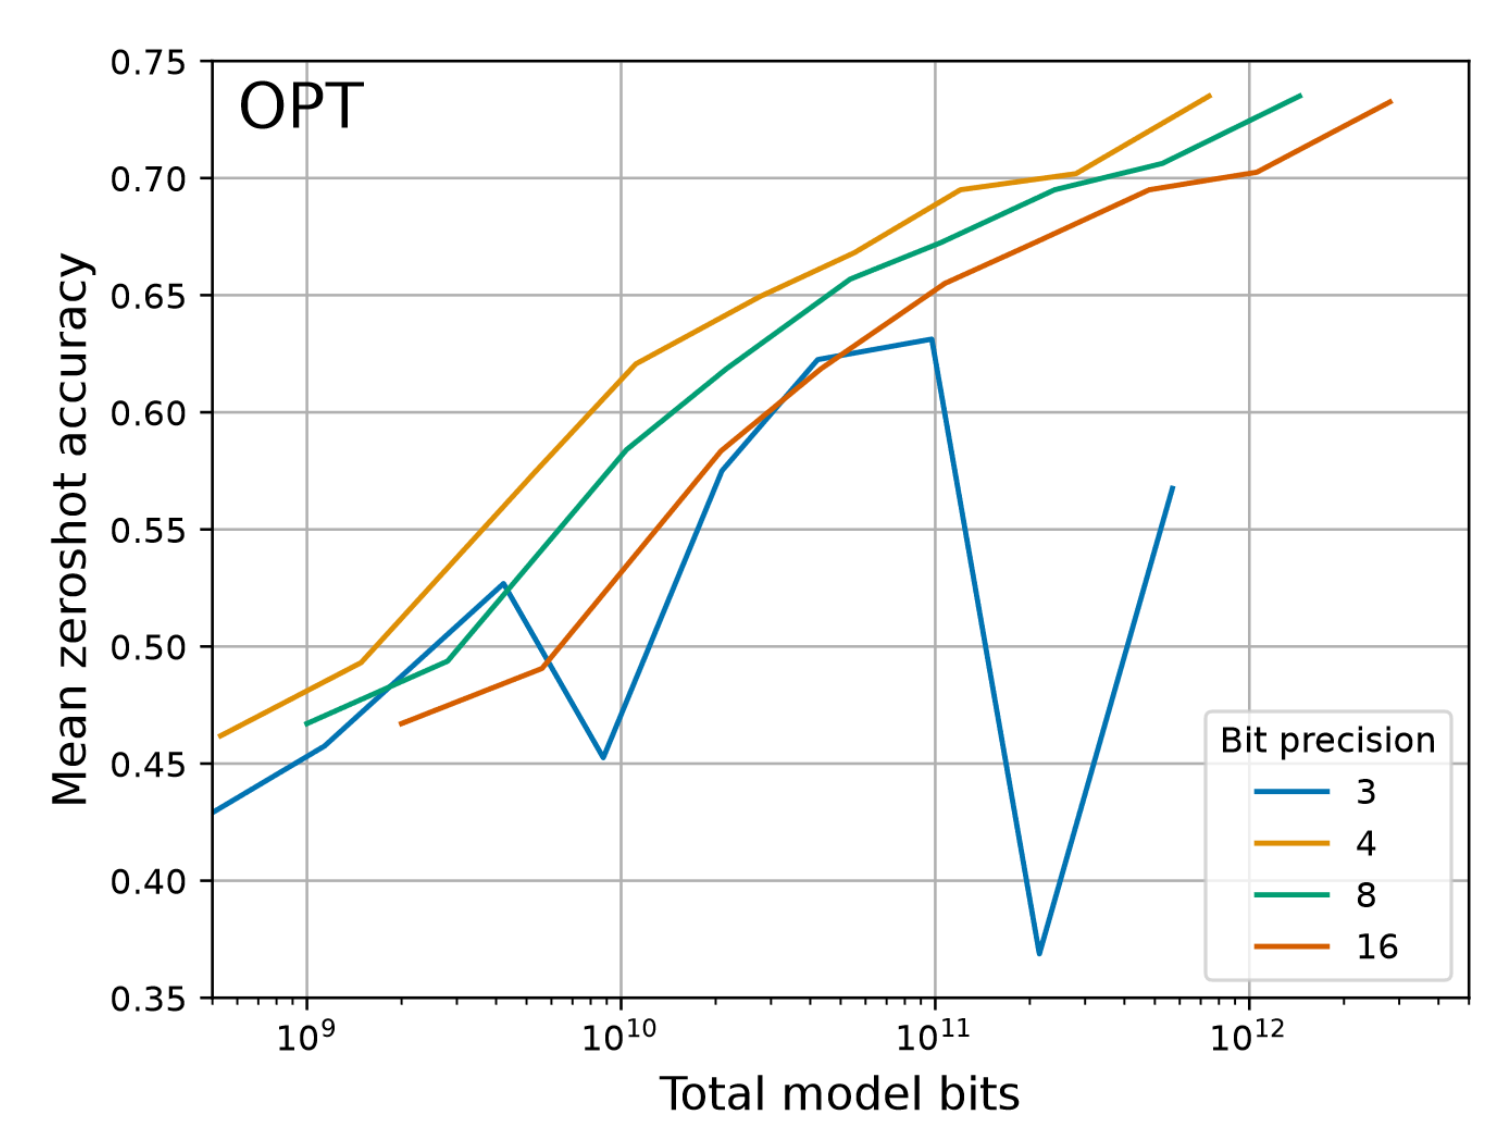
\includegraphics[width=\textwidth]{results/bit_scaling_laws.png}
    \caption[Korrektheit von OPT Modellen nach Modellbits]{Korrektheit von OPT Modellen aufgeteilt nach unterschiedlicher Bitanzahl pro Parameter aus \citet{4bit}. Modelle mit gleicher Parameteranzahl liegen ungefähr auf gleicher X-Achse, jedoch nicht auf gleicher Y-Achse.}%
    \label{fig:bit_scaling}
\end{figure}
Um große Modelle zu trainieren und zu nutzen, ist der Einsatz der \ac{zero}-Optimierung ein erster Schritt, der in \citet{deepspeed} vorgestellt wird.
Mit Hilfe der \ac{zero}-Stufe 3 Optimierung können Optimierungs- und Parameterzustände auf \ac{cpu}s und Festplatten ausgelagert werden, während die Berechnungen weiterhin auf \ac{gpu}s durchgeführt werden.
Zusätzlich kann durch eine Quantisierung der Modelle in kleinere Datentypen die Anzahl der benötigten \ac{gpu}-\ac{ram}s deutlich reduziert werden.
\citet{4bit} untersuchte den Einfluss der Quantisierung auf die Performance der Modelle und zeigte, dass eine Quantisierung auf 4 Bit die Leistung der Modelle nur geringfügig beeinflusst.
\cref{fig:bit_scaling} zeigt die Korrektheit von OPT-Modellen mit unterschiedlichen Datentypen (3, 4, 8 und 16 Bit).
Modelle mit gleicher Parameteranzahl liegen nicht auf dem gleichen Y-Achse, da die X-Achse in Modellbits angegeben ist.
Modelle mit der gleichen Anzahl von Parametern, aber einer geringeren Anzahl von Bits pro Parameter sind daher weiter links in der Grafik angeordnet.
Dennoch zeigen diese Abbildung von \citet{4bit} und ähnliche Abbildungen für andere Modelltypen eine fast identische Leistung bis einschließlich 4 Bit.\\

Zusätzlich ist es möglich, Modelle während der Inferenz in einen 8-Bit-Modus zu konvertieren, um Ressourcen zu sparen.
\citet{8bit-inference} haben gezeigt, dass bei der Verwendung von 8-Bit-Matrix-Multiplikationen keine signifikanten Leistungseinbußen zu erwarten sind.
Der 8-Bit Inferenzmodus wurde auch in dieser Arbeit verwendet, um die trainierten Modelle auf einer Nvidia Tesla A30 GPU mit \SI{24}{\giga\byte} \ac{ram} nutzen zu können.\\

\section{Human Reinforcement Learning}
Nach erfolgreichem Training eines Modells kann dessen Ausgabe wesentlich verbessert werden, indem Menschen die Ausgabe bewerten und das Modell entsprechend anpassen.
Dieser Schritt wurde auch bei GPT4 durchgeführt und ist einer der Gründe für die hohe Leistungsfähigkeit des Modells.
Mit Hilfe des so genannten Human Reinforcement Learning können Modelle darauf trainiert werden, Erklärungen zu ihren Antworten zu geben, unbeantwortete Fragen mit z.B. der generierten Antwort \enquote{Ich weiß es nicht} zu markieren, auf schädliche Inhalte nicht zu reagieren oder die Antwort zu verweigern und Texte klarer und freundlicher zu formulieren.
Dieser Trainingsschritt ist jedoch sehr aufwendig und kann nicht vollständig automatisiert werden.\\

Llama 2 verfügt über Versionen, die dieses Human Reinforcement Learning bereits durchlaufen haben.
In dieser Arbeit wird davon ausgegangen, dass dieses zusätzlich erlernte Wissen verloren geht, sobald ein Continual Pretraining durchgeführt wird.
Diese Annahme basiert auf der Tatsache, dass populäre Modelle das Human Reinforcement Learning als letzten Trainingsschritt durchlaufen haben.
Eine Widerlegung dieser Hypothese könnte potenziell auch die Leistung der Modelle verbessern.

\section{Datensatzvergrößerung}
Eine wesentliche Einschränkung der hier trainierten Modelle ist die Größe des Trainingsdatensatzes.
Mit etwa \num{34500} Tokens ist dieser Datensatz nicht mit den für das ursprüngliche Training verwendeten Datensätzen vergleichbar und erreicht nur eine Größe von \SI{600}{\kilo\byte}. Kleine Datensätze führen zu einer schnelleren Überanpassung, da der Datensatz mehrfach verwendet werden muss, bevor eine Anpassung des Modells an diesen erfolgen kann.
Dies zeigt sich auch in den Ergebnissen, da bereits nach 3 Epochen eine Überanpassung zu erkennen ist.
Größere Datensätze führen zu weniger Epochen und damit zu weniger Überanpassung.
Zudem enthalten größere Datensätze potentiell gleiche Informationen in unterschiedlicher Formulierung, was wiederum die Generalisierbarkeit des Modells verbessert.
Insbesondere die Kriterien Robustheit und Fragenverständnis profitieren von größeren Datensätzen.\\

Für die Verwendung größerer Datensätze wäre es optimal, weitere Literatur zum Thema Informationssysteme im Gesundheitswesen heranzuziehen.
Wichtig ist dabei, dass die Wissensinhalte identisch sind, so dass sich die Aussagen zwischen den Büchern nicht widersprechen.
Auch eine Zusammenstellung einzelner Kapitel aus verschiedenen Quellen mit gleichem Inhalt könnte die Größe des Datensatzes erhöhen und damit die Leistung der Modelle verbessern.\\

\section{Domänenspezifische Modelle}
Das Llama 2 Modell wurde ohne speziellen Fokus auf eine Domäne, insbesondere die Domäne Medizininformatik, trainiert.
Allgemein trainierte Modelle können einen breiteren Anwendungsbereich abdecken, enthalten aber auch weniger Verständnis einzelner Domänen als domänenspezifische Modelle.
Die Verwendung von Modellen, die stärker auf die Domäne der Medizininformatik oder auf wissenschaftliche Inhalte fokussiert sind, könnte die Basisleistung des Modells und damit auch die Endleistung der hier trainierten Modelle verbessern.\\

Leider existieren zum Zeitpunkt dieser Arbeit keine domänenspezifischen Modelle in der Größe von Llama 2, da entweder die Größe der Modelle oder die Größe des Datensatzes geringer ist.
Domänenspezifische Modelle können auch Informationen enthalten, die im Widerspruch zum verwendeten Trainingsdatensatz stehen, aber besser gelernt wurden, weil mehr Informationen im ursprünglichen Datensatz vorhanden waren.
Das bewusste Verlernen dieses falschen Wissens ist nicht trivial und kann die Leistung des Modells negativ beeinflussen.
Eine Möglichkeit der Modellanpassung wurde von \citet{knowledge_neurons} vorgestellt, um bestimmte Wissensneuronen aus einem Modell zu entfernen.

\section{Adapter-basiertes Training}\label{sec:adapter-training}
Wie bereits in \cref{ch:relatedWork} erwähnt, ist neben den klassischen Trainingsmethoden auch das Training mit Hilfe von Adaptern möglich.
\citet{adapterhub} stellt eine Plattform zur Verfügung, die es erlaubt, kleinere Neuronale Netze zwischen die Modellschichten einzufügen und diese zu trainieren.
Dies minimiert die benötigten Ressourcen, verkürzt die Trainingszeit und verhindert das Verlernen von Wissen.
Adapter müssen speziell für Modelltypen entwickelt werden und sind zum Zeitpunkt dieser Arbeit nicht für Llama-Modelle verfügbar.
Eine eigene Implementierung für die Llama Modelle könnte die endgültige Performance der Modelle verbessern.\\

Neben dem Einfügen von Adaptern ist auch die Verwendung von \ac{lora}, eingeführt in \citet{lora}, möglich.
\ac{lora} erlaubt das Einfügen von trainierbaren Matrizen in jede Schicht und hat ähnliche Vorteile wie Adapter.
Die Verwendung von \ac{lora} wurde im Rahmen dieser Arbeit untersucht, jedoch nicht in die endgültige Auswertung übernommen, da eine Inferenz nicht möglich war.

\section{Textextraktion aus Kontext}
Diese Arbeit konzentriert sich primär auf die Verwendung von Decoder-basierten Modellen zur Generierung von Antworten auf Fragen.
Grund dafür ist die potentiell höhere Generalisierbarkeit auf Formulierungen um besser generierten Text zu erhalten.
Neben der Generierung von Text ist auch die Extraktion von Text aus einem gegebenen Kontext eine mögliche Lösung.
Mit Hilfe von Encoder-basierten Modellen wie z.B. \ac{bert} ist es möglich, Textpassagen, die Antworten auf gegebene Fragen enthalten, aus einem Kontext zu extrahieren.
Dieser Ansatz könnte zu einer besseren Korrektheit der Fragen führen, allerdings könnten andere Kriterien wie Robustheit und Erklärbarkeit darunter leiden.\\

\section{Retrieval Augmented Generation}
Man könnte auch ganz auf das Training von Decoder-basierten Modellen verzichten, bei denen das Modell die Frage nur mit Hilfe eines gegebenen Kontextes beantworten soll.
Dieser Ansatz verspricht sehr gute Ergebnisse, da Modelle wie GPT4 bereits sehr gute Leistungen bei der Extraktion von Informationen aus Kontexten zeigen.\\

\citet{context-extract} haben dieses Verhalten an großen Sprachmodellen untersucht und gezeigt, dass Modelle in der Lage sind, Informationen aus Anfang und Ende eines Kontextes weitgehend korrekt zu extrahieren.
Um nur den Kontext zur Beantwortung von Fragen zu verwenden, müssen Modelle mit einer großen Kontextlänge gewählt und das verwendete Buch optional gekürzt werden. \citet{extending-context} beschreibt eine Möglichkeit, die verfügbare Kontextlänge mit Hilfe von positionsabhängiger Interpolation zu erweitern.\\
Eine Kombination aus einem Encoder-basierten Modell zur Bestimmung der Textposition und einem Decoder-basierten Modell zur Generierung einer Antwort mit Hilfe der extrahierten Textposition könnte ebenfalls Abhilfe schaffen. Dieser Ansatz wurde von \citet{retrieval-1} untersucht und erzielte \ac{sota} Ergebnisse in drei \ac{qa} Evaluationsdatensätzen. Ähnliche Ergebnisse wurden von \citet{retrieval-2} in ihrem Artikel erreicht.\\

Dieser Ansatz erfordert kein weiteres Training von Modellen und führt dementsprechend zu deutlich weniger Leistungsanforderungen. Das bedeutet, dass größere Modelle unter gleicher Hardware genutzt werden können und damit auch die erwarteten Ergebnisse höher ausfallen könnten. Die Komplexität liegt hierbei in der Integration der Modelle zu einem Gesamtsystem und der Veränderung bereits existierender Modelle um größere Kontextlängen zu ermöglichen.

\section{Zusammenfassung}
Die hier vorgestellten Richtungen für zukünftige Arbeiten versprechen eine Verbesserung der Leistung der Modelle in vielerlei Hinsicht.
Zum besseren Überblick stell \cref{tab:future-work} eine Übersicht über die hier vorgestellten Ansätze dar.
Die Tabelle ist nach Erfolgseinschätzung sortiert.
Ein hoher Aufwand bedeutet grundlegende strukturelle Änderungen im genutzten Prozess und erfordert dementsprechend hohen Zeit- und Kostenaufwand.

\begin{table}
    \centering
    \resizebox{\textwidth}{!}{%
    \begin{tabular}{lll}
        \toprule
        \textbf{Ansatz}                   & \textbf{Aufwand} & \textbf{Erfolgseinschätzung}             \\
        \midrule
        Retrieval Augmented Generation    & hoch                                          & sehr hoch \\
        Datensatzvergrößerung             & niedrig                                       & hoch      \\
        Modellvergrößerung                & hoch                                          & hoch      \\
        Human Reinforcement Learning      & sehr hoch                                     & hoch      \\
        Domänenspezifische Modelle        & niedrig                                       & mittel    \\
        Textextraktion aus Kontext        & niedrig                                       & mittel    \\
        Adapter-basiertes Training        & mittel                                        & mittel    \\
    \end{tabular}}
    \caption[Verbesserungsansätze der Modelle]{Übersicht über mögliche Ansätze zur Verbesserung der Leistung der Modelle}\label{tab:future-work}
\end{table}

% ********************************************************************
% Backmatter
%*******************************************************
\cleardoublepage%*******************************************************
% Summary
%*******************************************************
\pdfbookmark[1]{Zusammenfassung}{summary}
\chapter*{Zusammenfassung}
\addcontentsline{toc}{chapter}{Zusammenfassung}
\markboth{\spacedlowsmallcaps{Zusammenfassung}}{\spacedlowsmallcaps{Zusammenfassung}}
Die Wissensbeschaffung in der Medizininformatik ist ein komplexer und wichtiger Bestandteil von Forschung, Lehre und Praxis.
Umso wichtiger ist die Effizienz und Qualität der Wissensbeschaffung.
Informationssysteme stellen dabei eine grundlegende Architektur in diesem Bereich dar.
Das Buch \citetitle{bb} von \citet{bb} enthält eine umfassende Einführung in die Thematik der Informationssysteme in der Medizin.
Die Extraktion von Informationen und Wissen aus dem Buch erweist sich jedoch als schwierig.
In dieser Arbeit wurde ein vortrainiertes Sprachmodell verwendet, um den Inhalt des Buches effizienter und leichter zugänglich zu machen.
Ziel ist es, Wissen aus dem Buch zu extrahieren.
Dieses Ziel wurde anhand von Prüfungsfragen aus dem Buch und Modulen der Universität Leipzig, die inhaltlich auf dem Buch aufbauen, evaluiert.\\

Um diese Ziele zu erreichen, wurden verschiedene Sprachmodelle auf ihre Eignung verglichen.
Die Wahl fiel auf das Sprachmodell Llama 2 von MetaAI \citep{llama2}.
Dieses vortrainierte Sprachmodell wurde mit Hilfe des Continual Pretrainings weiter auf das Buch trainiert.
Während des Trainings wurde die Qualität des Modells zu verschiedenen Zeitpunkten evaluiert.
Diese Bewertung basierte auf den Kriterien Korrektheit, Erklärbarkeit, Fragenverständnis und Robustheit.
Abschließend wurde ein Vergleich zwischen den Trainingszeitpunkten, dem nicht weiter trainierten Modell und dem \ac{sota} Modell GPT4 durchgeführt.\\

\enlargethispage{0.5\baselineskip}
Die Ergebnisse zeigen, dass Modelle mit Hilfe von Continual Pretraining auf ein spezifisches Buch trainiert werden können und in fast allen Kriterien bessere Ergebnisse erzielen als das nicht weiter trainierte Modell.
Aufgrund des Größenunterschieds zwischen GPT4 und dem hier verwendeten Modell Llama 2 7B wird die Leistung von GPT4 jedoch nicht erreicht.
Das nicht weiter trainierte Modell erreichte nur einen MakroF1-Wert von \num{0.1} und konnte durch das hier durchgeführte Training auf \num{0.33} gesteigert werden.
Dies zeigt das Potential dieser Methode.
Allerdings sind die Modelle noch nicht mit dem \ac{sota} Modell GPT4 vergleichbar, das einen MakroF1-Wert von \num{0.7} erreichte.
Die hier trainierten Modelle stellen keinen für die Praxis nutzbaren Zustand dar, lösen aber die gestellte Zielstellung \enquote{Machbarkeit der Beantwortung von Fragen mit Hilfe von Sprachmodellen}.
Ausführliche Ergebnisgrafiken und die verwendeten Skripte stehen unter \url{https://doi.org/10.5281/zenodo.8363501} zur Verfügung.\\

Um die Leistungsfähigkeit von Sprachmodellen zu erhöhen, können sowohl die Modellgröße als auch die Größe des Datensatzes erhöht werden.
Auch neue Entwicklungen im Bereich der Adapter (\cref{sec:adapter-training}) zeigen ressourceneffiziente Ansätze, um die Performanz von Sprachmodellen zu steigern.
Insbesondere der Einsatz von Retrieval-Augmented Generation bieten vielversprechende Erweiterungsmöglichkeiten.\\

Zusammenfassend kann gesagt werden, dass die Leistung von Sprachmodellen bei der Beantwortung von Klausurfragen durch Continual Pretraining gesteigert werden kann, auch wenn die Endleistung noch keinen praxistauglichen Zustand erreicht.
So ist die Lösung einer Beispielklausur durch die Modelle nicht vollständig möglich, ebenso können Fragen zu Informationssystemen im Gesundheitswesen nur teilweise beantwortet werden.
Die Schwierigkeit der Wissensbeschaffung aus \citet{bb} kann durch die Modelle erleichtert werden, insbesondere die Zusammenführung fragmentierter Definitionen, erreicht aber keinen in der Praxis nutzbaren Zustand, weshalb die Wissensbeschaffung aus dem Buch weiterhin schwierig bleibt.\\

\vfill

\cleardoublepage%********************************************************************
% Bibliography
%*******************************************************
% work-around to have small caps also here in the headline
% https://tex.stackexchange.com/questions/188126/wrong-header-in-bibliography-classicthesis
% Thanks to Enrico Gregorio
\defbibheading{bibintoc}[\bibname]{%
  \phantomsection
  \manualmark
  \markboth{\spacedlowsmallcaps{#1}}{\spacedlowsmallcaps{#1}}%
  \addtocontents{toc}{\protect\vspace{\beforebibskip}}%
  \addcontentsline{toc}{chapter}{\tocEntry{#1}}%
  \chapter*{#1}%
}
%\bibliographystyle{dinat}
\printbibliography[heading=bibintoc]

\appendix
\renewcommand{\thechapter}{\alph{chapter}}
\cleardoublepage
\part*{Appendix}
%*****************************************
\pdfbookmark[1]{Appendinx}{appendix}
\chapter*{Appendix}\label{ch:appendix}
%*****************************************
\section*{Evaluierungsdatensatz}\label{app:evaldata}
Im Folgenden werden die verwendeten Evaluationsdatensätze vorgestellt, die zur Berechnung der Kriterien in \cref{ch:results} verwendet wurden.
Die Evaluationsdatensätze sind unterteilt in Einzelfaktfragen (\cref{tab:evaldata-single}), Multifakten-Fragen (\cref{tab:evaldata-multi}) und Transferfragen (\cref{tab:evaldata-transfer}).
Während der Evaluation wurden allen Modellen dieselben Fragen gestellt.
Ihre Antworten wurden mit den hier gegebenen Antworten verglichen und ausgewertet.
{\footnotesize
\begin{landscape}
\begin{longtable}{p{3cm}p{1.7\textwidth}}
    \toprule
    \multicolumn{2}{c}{\textbf{Evaluierungsdatensatz (Einzelfaktfragen)}}\\
    \midrule
    Frage & In Sect. 4.2, we introduced a three-dimensional classification of activities of management of information systems.
    How would you describe the scope and tasks of the following activities of managing information systems? - Developing a strategic information management plan (e.g., this is related to strategic planning), \\
    Umformuliert & How would you describe the scope and tasks of the following activities of managing information systems: Developing a strategic information management plan \\
    Antwort & Developing a strategic information management plan: strategic planning \\
    Quelle|Anz. Antw. & Book | 1\\
    \midrule
    Frage & - Initiating projects from the strategic project portfolio, \\
    Umformuliert & How would you describe the scope and tasks of the following activities of managing information systems: Initiating projects from the strategic project portfolio \\
    Antwort & Initiating projects from the strategic project portfolio: strategic directing \\
    Quelle|Anz. Antw. & Book | 1 \\
    \midrule
    Frage & - Collection and analysis of data from user surveys on their general satisfaction with the health information system, \\
    Umformuliert & How would you describe the scope and tasks of the following activities of managing information systems: Collection and analysis of data from user surveys on their general satisfaction with the health information system \\
    Antwort & Collecting and analyzing data from user surveys on their general health information system's satisfaction: strategic monitoring \\
    Quelle|Anz. Antw. & Book | 1 \\
    \midrule
    Frage & - Planning a project to select and introduce a new CPOE system, \\
    Umformuliert & How would you describe the scope and tasks of the following activities of managing information systems: Planning a project to select and introduce a new CPOE system \\
    Antwort & Planning a project to select and introduce a new CPOE system: tactical planning \\
    Quelle|Anz. Antw. & Book | 1 \\
    \midrule
    Frage & - Executing work packages within an evaluation project of a CPOE system, \\
    Umformuliert & How would you describe the scope and tasks of the following activities of managing information systems: Executing work packages within an evaluation project of a CPOE system \\
    Antwort & Executing work packages within an evaluation project of a CPOE system: tactical directing \\
    Quelle|Anz. Antw. & Book | 1 \\
    \midrule
    Frage & - Assessment of user satisfaction with a new intensive care system, \\
    Umformuliert & How would you describe the scope and tasks of the following activities of managing information systems: Assessment of user satisfaction with a new intensive care system \\
    Antwort & Assessment of user satisfaction with a new intensive care system: tactical monitoring \\
    Quelle|Anz. Antw. & Book | 1 \\
    \midrule
    Frage & - Planning of a user service desk for a group of clinical application components, \\
    Umformuliert & How would you describe the scope and tasks of the following activities of managing information systems: Planning of a user service desk for a group of clinical application components \\
    Antwort & Planning of a user service desk for a group of clinical application components: operational planning \\
    Quelle|Anz. Antw. & Book | 1 \\
    \midrule
    Frage & - Operation of a service desk for a group of clinical application components, \\
    Umformuliert & How would you describe the scope and tasks of the following activities of managing information systems: Operation of a service desk for a group of clinical application components \\
    Antwort & Operation of a service desk for a group of clinical application components: operational directing \\
    Quelle|Anz. Antw. & Book | 1 \\
    \midrule
    Frage & - Daily monitoring of network availability and network failures.\\
    Umformuliert & How would you describe the scope and tasks of the following activities of managing information systems: Daily monitoring of network availability and network failures \\
    Antwort & Daily monitoring of network availability and network failures: operational monitoring \\
    Quelle|Anz. Antw. & Book | 1 \\
    \midrule
    Frage & Definieren Sie den Begriff ``Krankenhausinformationssystem''. \\
    Umformuliert & Define the term ``hospital information system''. \\
    Antwort & A Hospital Information system is the socio-technical subsystem of for hospitals.
    It comprises all data, information, and knowledge processing as well as the associated human or technical actors in their respective data, information, and knowledge processing roles.\\
    Quelle|Anz. Antw. & IS\_2022\_07\_18 | 1 \\
    \midrule
    Frage & Wie erhalten Apotheker:innen Zugriff auf verordnete eRezepte? \\
    Umformuliert & How do pharmacists get access to e-prescriptions? \\
    Antwort & Via the CPOE System within a hospital.
    Extern via their own pharmacists information system.\\
    Quelle|Anz. Antw. & IS\_2022\_07\_18 | 1 \\
    \midrule
    Frage & Definieren Sie den Begriff ``transinstitutionelles Gesundheitsinformationssystem''. Verwenden Sie dabei den Begriff des ``Settings''. \\
    Umformuliert & Define the term ``trans-institutional health information system''. Use the term ``setting'' for this purpose.\\
    Antwort & A transinstitutional health information system is the socio-technical subsystem which comprises all data, information, and knowledge processing as well as the associated human or technical actors in their respective data, information, and knowledge processing roles.
    It describes the information system of a health care network, in which multiple Settings are present.
    Each setting is a context this information system is used in, for example in the stationary or ambulant care, but also rehabilitation or care of the elder.\\
    Quelle|Anz. Antw. & IS\_2022\_09\_27 | 1 \\
    \midrule
    Frage & tHIS? \\
    Umformuliert & Define the term ``tHIS''. \\
    Antwort & tHIS stands for transinstitutional health information system, an information system of a health care network which consists of multiple health care settings (contexts). It comprises all data, information, and knowledge processing as well as the associated human or technical actors in their respective data, information, and knowledge processing roles.\\
    Quelle|Anz. Antw. & IS\_2022\_09\_27 | 1 \\
    \midrule
    Frage & Was ist ein Arztbrief? \\
    Umformuliert & What is a doctor's letter? \\
    Antwort & A doctor's letter is a transfer document for communication between doctors.
    It is a form of information for the referring doctor, who has arranged for a referral to a hospital or other medical treatment in the outpatient sector or for the further treating doctor who takes over the further treatment.
    The doctor's letter provides a summary overview of the patient's status at discharge, a review of the course of the disease, the therapy initiated, an interpretation of the events related to the course of the disease in the specific case, information on the classification of the disease according to ICD, OPS, ICF and possibly also DRG and recommendations for continuing therapy.\\
    Quelle|Anz. Antw. & IS\_2022\_09\_27 | 1 \\
    \midrule
    Frage & Was ist openEHR \\
    Umformuliert & What is openEHR? \\
    Antwort & openEHR is an open standard specification in health informatics that describes the management and storage, retrieval and exchange of health data in electronic health records (EHRs). In openHER, all health data for a person is stored in a ``one lifetime'', vendor-independent, person-centred EHR.
    It is completely model-driven, and separates domain semantics out from software, into models created by domain professionals.\\
    Quelle|Anz. Antw. & IS\_2022\_09\_27 | 1 \\
    \midrule
    Frage & Was ist ein Archetype? \\
    Umformuliert & What is an archetype in the context of health information systems? \\
    Antwort & An archetype is a formal specification of a clinical concept that can be used to create interoperable and reusable electronic health records.
    Archetypes are designed to be independent of any specific EHR system and are intended to be used as building blocks for EHRs.\\
    Quelle|Anz. Antw. & IS\_2022\_09\_27 | 1 \\
    \midrule
    Frage & Ist openEHR ein Standard? \\
    Umformuliert & Is openEHR a standard? \\
    Antwort & Yes, openEHR is an open standard specification in health informatics that describes the management and storage, retrieval and exchange of health data in electronic health records.\\
    Quelle|Anz. Antw. & IS\_2022\_09\_27 | 1 \\
    \midrule
    Frage & Könnte man mit Hilfe von openEHR eine (DB1, ACn, Vn)-Architektur realisieren? \\
    Umformuliert & Could one realise a DB\textasciicircum{}1, AC\textasciicircum{}n, V\textasciicircum{}n architecture with the help of openEHR? \\
    Antwort & Yes \\
    Quelle|Anz. Antw. & IS\_2022\_09\_27 | 1 \\
    \midrule
    Frage & Was ist ein Modell? \\
    Umformuliert & What is a model in the context of health information systems? \\
    Antwort & A model is a representation of a system or process that is used to help understand and predict the behavior of the system or process.
    Health information systems models can be used to help design and evaluate health information systems.
    They can also be used to help identify areas for improvement in health information systems.\\
    Quelle|Anz. Antw. & IS\_2022\_09\_27 | 1 \\
    \midrule
    Frage & Was ist ARIS? \\
    Umformuliert & What is ARIS? \\
    Antwort & The Architecture of Integrated Information Systems is a framework for describing business processes.
    It provides modeling methods and meta-structures that are comprised in information models.\\
    Quelle|Anz. Antw. & IS\_2022\_09\_27 | 1 \\
    \midrule
    Frage & Wie kann man dynamische Aspekte von IS modellieren? \\
    Umformuliert & How can dynamic aspects of Information Systems be modelled? \\
    Antwort & With a Business Process Model such as BPMN \\
    Quelle|Anz. Antw. & IS\_2022\_09\_27 | 1 \\
    \midrule
    Frage & Was ist IHE? \\
    Umformuliert & What is IHE? \\
    Antwort & IHE stands for Integrating the Healthcare Enterprise.
    It is an initiative by healthcare professionals and industry to improve the way computer systems in healthcare share information.
    IHE promotes the coordinated use of established standards such as DICOM and HL7 to address specific clinical needs in support of optimal patient care \\
    Quelle|Anz. Antw. & IS\_2022\_09\_27 | 1 \\
    \midrule
    Frage & Was tut ein Kommunikationsserver? \\
    Umformuliert & What does a communication server do  in the context of health information systems? \\
    Antwort & A communication server in the context of health information systems is a server that enables communication between different systems.
    It is responsible for routing messages between different applications and systems.
    It can also be used to manage the flow of data between different systems.\\
    Quelle|Anz. Antw. & IS\_2022\_09\_27 | 1 \\
    \midrule
    Frage & Wozu setzt man Remote Function Calls ein? \\
    Umformuliert & What are Remote Function Calls used for? \\
    Antwort & Remote Function Calls (RFC) is a communications interface based on CPI-C, but with more functions and easier for application programmers to use.
    It is the call or remote execution of a Remote Function Module in an external system.
    In the SAP system, these functions are provided by the RFC interface system.
    The RFC interface system enables function calls between two SAP systems \\
    Quelle|Anz. Antw. & IS\_2022\_09\_27 | 1 \\
    \midrule
    Frage & Wie findet ein Labormitarbeiter mit einer Fallnummer in der Hand Geburtsdatum und Geschlecht eines Patienten? \\
    Umformuliert & How does a lab worker with a case number in hand find a patient's date of birth and gender? \\
    Antwort & In the Laboratory Information System, which got its information from a communication server.\\
    Quelle|Anz. Antw. & IS\_2022\_09\_27 | 1 \\
    \midrule
    Frage & Erläutern Sie die Taxonomy für Krankenhausinformationssysteme! \\
    Umformuliert & Explain the taxonomy for hospital information systems! \\
    Antwort & The taxonomy for HIS is a classification system that is used to categorize different types of HIS based on their functionality and purpose.
    The taxonomy can be used to help healthcare organizations select the right HIS for their needs.
    There are several different taxonomies for HIS, but they generally include categories such as clinical information systems, administrative information systems, and decision support systems \\
    Quelle|Anz. Antw. & IS\_2022\_09\_27 | 1 \\
    \midrule
    Frage & Wieso haben wir meist (ACn, Vn)? \\
    Umformuliert & Why do we mostly have (AC\textasciicircum{}n, V\textasciicircum{}n)? \\
    Antwort & This allows Best of Breed Architecture choosing the best products and being independent from vendors.\\
    Quelle|Anz. Antw. & IS\_2022\_09\_27 | 1 \\
    \midrule
    Frage & Wie kann man auch bei fehlender Vollausleuchtung mit den allgegenwärtigen Funklöchern hinter metallwagen so umgehen, dass Mobile Anwendungen nicht laufend abstürzen? \\
    Umformuliert & Even in the absence of full coverage, how can you deal with the ubiquitous radio holes behind metal trolleys in such a way that mobile applications don't crash all the time? \\
    Antwort & One of this:
    - caching and local storage
    - Offline Mode
    - Background Syncing and Queuing \\
    Quelle|Anz. Antw. & IS\_2022\_09\_27 | 1 \\
    \midrule
    Frage & Welche Speichermedien gewährleisten eine Unveränderbarkeit der Daten? \\
    Umformuliert & Which storage media guarantee that the data cannot be changed? \\
    Antwort & Write once read many (WORM) data such as Optical Discs, Tape Drives, Solid State Drives or Memory cards \\
    Quelle|Anz. Antw. & IS\_2022\_09\_27 | 1 \\
    \midrule
    Frage & Ist ``Dokumentation'' eine datenverarbeitende Aufgabe bzw.
    eine enterprise function? \\
    Umformuliert & Is ``documentation'' a data processing task or an enterprise function? \\
    Antwort & A data processing task \\
    Quelle|Anz. Antw. & IS\_2022\_09\_27 | 1 \\
    \midrule
    Frage & Mit welchem Anwendungssystem wird im UKL die Anforderung von Laborleistungen  (order entry) unterstützt? \\
    Umformuliert & Which application system is used in the University Hospital to support the request for laboratory services (order entry)? \\
    Antwort & Laboratory Information System \\
    Quelle|Anz. Antw. & IS\_2022\_09\_27 | 1 \\
    \midrule
    Frage & Wie erfolgt die Kommunikation der Anforderung (order) an das LIS? \\
    Umformuliert & How is the request (order) communicated to the LIS? \\
    Antwort & It isn't. The call is made from the work place during the context integration of patient identifying data to the LIS.\\
    Quelle|Anz. Antw. & IS\_2022\_09\_27 | 1 \\
    \midrule
    Frage & Mit welchem Anwendungssystem wird im UKL ein Laborbefund (finding) angezeigt? \\
    Umformuliert & Which application system is usually used to display a laboratory finding in the University Hospital? \\
    Antwort & (COPRA, LIS direkt!) \\
    Quelle|Anz. Antw. & IS\_2022\_09\_27 | 1 \\
    \midrule
    Frage & Wie würden sie die PWE eines KIS gestalten? \\
    Umformuliert & How would they design the physical tool layer of a HIS? \\
    Antwort & Redundancy by mirror servers \\
    Quelle|Anz. Antw. & A\_2021 | 1\\
\bottomrule
\caption*{Evaluierungsdatensatz (Einzelfaktfragen)}\label{tab:evaldata-single}
\end{longtable}
\end{landscape}

\begin{landscape}
    \begin{longtable}{p{3cm}p{1.7\textwidth}}
    \toprule
    \multicolumn{2}{c}{\textbf{Evaluierungsdatensatz (Multifakten-Fragen)}}\\
    \midrule
    Frage & Was ist der Unterschied zwischen dem PVS und dem PDMS? \\
    Umformuliert & What is the difference between the PMS and the PDMS? \\
    Antwort & PMS:
    - primary focus on helping health care provides streamline their day-to-day tasks

    PDMS:
    - primary focus on capturing maintaining comprehensive and accurate patient medical data.\\
    Quelle|Anz. Antw. &  IS\_2022\_09\_27  | 2 \\
    \midrule
    Frage & Look at the entity type ``patient'' that is interpreted and updated by various functions.
    Which functions update the patient information, which functions interpret it? \\
    Umformuliert & Look at the entity type ``patient'' that is interpreted and updated by various functions to be performed by health care professionals and other staff in health care facilities.
    Which functions update the patient information, which functions interpret it? \\
    Antwort & The entity type ``patient'' is updated by the function ``patient admission.'' All other functions that are related to patient care interpret it.\\
    Quelle|Anz. Antw. &  Book  | 2 \\
    \midrule
    Frage & Look at the 3LGM\textasciicircum{}2 example in Sect. 2.15.
    Use this example to explain the meaning of the following elements: functions, entity types, application systems, non-computer-based application components, physical data processing system, and inter-layer relationships.\\
    Umformuliert & Use the provided example to explain the meaning of the following elements: functions, entity types, application systems, non-computer-based application components, physical data processing system, and inter-layer relationships.\\
    Kontext & Example: Four subfunctions of patient admission (appointment scheduling, patient identification and checking for readmitted patients, administrative admission, and visitor and information services) are supported by the patient administration system, which is a part of the ERPS.
    Medical admission and nursing admission are supported by the MDMS.
    Obtaining consent for processing of patient-related data is supported by the non-computer-based application component for patient data privacy forms.
    This application component is based on paper forms which are scanned by a clerk (see physical tool layer) and then stored in the MDMS.

    The patient administration system, which is the master application system (Sect. 3.9.1) for the entity type ``patient,'' sends the administrative patient data as a message to the MDMS.
    The MDMS can thus store this information about the entity type ``patient'' in its own database; administrative patient data that is needed to support medical admission and nursing admission as functions therefore do not have to be reentered in the MDMS.
    The entity type ``patient'' is both stored in the database systems of the ERPS and the MDMS what is represented by dashed lines between the domain layer and the logical tool layer.

    Both the patient administration system and the MDMS are run on servers at a virtualized server farm (see relationships between logical and physical tool layer). The application systems can be accessed by different end devices (patient terminal, PC, tablet PC).

    It therefore simplifies some aspects which might be relevant in other contexts.
    Another visualization of relationships between 3LGM\textasciicircum{}2 model elements is the matrix view.
    The patient administration system supports three different functions, the MDMS supports two functions, and one function is supported by the paper-based patient data privacy form system.
    The matrix view also helps to identify incomplete parts of models.
    We can see that there are no functions modeled that are supported by the financial accounting system, the human resources management system, and the material management system, which are parts of the ERPS.

    The matrix view is an alternative representation of configuration lines between functions at the domain layer and application components at the logical tool layer.
    Matrix views are also available for visualizing relations between other pairs of connected 3LGM\textasciicircum{}2 classes.\\
    Antwort & Administrative admission is an enterprise function that is supported by the patient administration system.
    One entity type that is used and updated by this function is ``patient.'' The paper-based patient data privacy form system is an example of a non-computer-based application component.
    The virtualized server farm is an example of a physical tool.
    The inter-layer relationships of this example show which functions are supported by which application system and which physical data processing system the application systems are installed on.\\
    Quelle|Anz. Antw. &  Book  | 6 \\
    \midrule
    Frage & Look at the 3LGM\textasciicircum{}2 sample model in Sect. 2.15 and try to answer the following questions.

    (a) Find examples of specialization or decomposition at the domain layer.

    (b) What is the meaning of the arrows pointing from patient identification to ``patient'' and from ``patient'' to medical admission?

    (c) What entity type that is stored in the paper-based patient data privacy form system should be added at the domain layer?

    (d) Why is the function patient admission not connected with any application system?

    (e) Which physical data processing systems are needed for the function ``obtaining patient consent for the processing of data''? \\
    Umformuliert & Answer the following questions under the given example context.
    (a) Find examples of specialization or decomposition at the domain layer.

    (b) What is the meaning of the arrows pointing from patient identification to ``patient'' and from ``patient'' to medical admission?

    (c) What entity type that is stored in the paper-based patient data privacy form system should be added at the domain layer?

    (d) Why is the function patient admission not connected with any application system?

    (e) Which physical data processing systems are needed for the function ``obtaining patient consent for the processing of data''? \\
    Kontext & Four subfunctions of patient admission (appointment scheduling, patient identification and checking for readmitted patients, administrative admission, and visitor and information services) are supported by the patient administration system, which is a part of the ERPS.
    Medical admission and nursing admission are supported by the MDMS.
    Obtaining consent for processing of patient-related data is supported by the non-computer-based application component for patient data privacy forms.
    This application component is based on paper forms which are scanned by a clerk (see physical tool layer) and then stored in the MDMS.

    The patient administration system, which is the master application system (Sect. 3.9.1) for the entity type ``patient,'' sends the administrative patient data as a message to the MDMS.
    The MDMS can thus store this information about the entity type ``patient'' in its own database; administrative patient data that is needed to support medical admission and nursing admission as functions therefore do not have to be reentered in the MDMS.
    The entity type ``patient'' is both stored in the database systems of the ERPS and the MDMS what is represented by dashed lines between the domain layer and the logical tool layer.

    Both the patient administration system and the MDMS are run on servers at a virtualized server farm (see relationships between logical and physical tool layer). The application systems can be accessed by different end devices (patient terminal, PC, tablet PC).

    It therefore simplifies some aspects which might be relevant in other contexts.
    Another visualization of relationships between 3LGM\textasciicircum{}2 model elements is the matrix view.
    The patient administration system supports three different functions, the MDMS supports two functions, and one function is supported by the paper-based patient data privacy form system.
    The matrix view also helps to identify incomplete parts of models.
    We can see that there are no functions modeled that are supported by the financial accounting system, the human resources management system, and the material management system, which are parts of the ERPS.

    The matrix view is an alternative representation of configuration lines between functions at the domain layer and application components at the logical tool layer.
    Matrix views are also available for visualizing relations between other pairs of connected 3LGM\textasciicircum{}2 classes.\\
    Antwort & (a) The function ``patient admission'' is decomposed into five subfunctions - patient admission is only complete if all the subfunctions are completed.
    The entity type ``patient'' is decomposed into four entity types - data regarding that entity type are only complete if data about all sub-entity types is complete.
    There are no examples of specialization at the domain layer of Fig. 2.11.

    (b) The function ``patient identification'' updates the entity type ``patient.'' The function ``medical admission'' uses the entity type ``patient.'' This indicates that identifying patient data are updated or created during patient admission and then used for medical admission.
        
    (c) The entity type ``privacy statement'' could be added at the domain layer.
    It would be updated by the function ``obtaining consent for processing of patient data.''
        
    (d) Patient admission is decomposed into five subfunctions with each being linked to an application component by which it is supported.
    Therefore, it could lead to an ambiguous model if the superordinated function was linked with another application component.
    The corresponding modeling rule says that only the leaf functions in a function hierarchy should be linked to application components.
        
    (e) The function ``obtaining patient consent for the processing of data'' is supported by the paper-based patient data privacy form system.
    For this, a paper record cabinet, a scanner, and a clerk handling these tools are the physical data processing systems needed for the function.\\
    Quelle|Anz. Antw. &  Book  | 5 \\
    \midrule
    Frage & Imagine a hospital information system that comprises four application systems: a PAS, an MDMS, a RIS, and a PDMS.
    The hospital is now considering the introduction of a communication server to improve data integration.
    Discuss the short-term and long-term pros and cons of this decision.
    Which syntactic and semantic standards could be used? \\
    Umformuliert & Imagine a hospital information system that comprises four application systems: a PAS, an MDMS, a RIS, and a PDMS.
    The hospital is now considering the introduction of a communication server to improve data integration.
    Discuss the short-term and long-term pros and cons of this decision.
    Which syntactic and semantic standards could be used? \\
    Antwort & Short-term advantages: The communication server can handle the communication between all four application systems, including receiving, buffering, transforming, and multicasting of messages.
    It can also be used for monitoring the communication traffic.
    The communication server thus supports data integration in heterogeneous information system architectures.

    Long-term advantages: In the resulting (ACn, CP1) architecture, new application components can easily be integrated, as only one communication interface to the communication server needs to be implemented.

    Standards: For the exchange of administrative data, HL7 V2 or V3 could be used as syntactic or semantic standard.
    For the exchange of clinical data, various communication standards can be chosen such as HL7 FHIR, DICOM for medical images, or HL7 CDA for clinical documents.\\
    Quelle|Anz. Antw. &  Book  | 3 \\
    \midrule
    Frage & The following questions can be answered by reading the text and analyzing the 3LGM\textasciicircum{}2 figures of the CityCare Example 3.11.

    (a) The EHRS and the VNA in CityCare are not linked with any function they support.
    Which function of the domain layer may (partly) be supported by these application systems? Which functions (as introduced in Sect. 3.3) that are supported by these application systems could be added at the domain layer?

    (b) In which database systems shown in the logical tool layer should the entity type ``patient'' be stored?

    (c) The MPI should receive messages containing PINs (entity type ``patient'') from all patient administration systems.
    Why is there no communication link between the MPI and the patient administration system of Ernst Jokl Hospital?

    (d) According to the matrix view, which functions are supported redundantly in CityCare? Discuss pros and cons of the functional redundancies in this scenario.
    What redundancies would you resolve and how?

    (e) Which functions in which health care facility cannot be performed anymore if ``Application Server 1 Ernst Jokl Hospital'' fails? Suggest a change to the physical tool layer that would minimize the risk of missing function support in case a single application server fails.

    (f) For the CityCare network, would it make sense to implement further profiles from IHE? Explain your decision.\\
    Umformuliert & The following questions can be answered reading the provided text.
    (a) The EHRS and the VNA in CityCare are not linked with any function they support.
    Which function of the domain layer may (partly) be supported by these application systems? Which functions (as introduced in Sect. 3.3) that are supported by these application systems could be added at the domain layer?

    (b) In which database systems shown in the logical tool layer should the entity type ``patient'' be stored?

    (c) The MPI should receive messages containing PINs (entity type ``patient'') from all patient administration systems.
    Why is there no communication link between the MPI and the patient administration system of Ernst Jokl Hospital?

    (d) According to the matrix view, which functions are supported redundantly in CityCare? Discuss pros and cons of the functional redundancies in this scenario.
    What redundancies would you resolve and how?

    (e) Which functions in which health care facility cannot be performed anymore if ``Application Server 1 Ernst Jokl Hospital'' fails? Suggest a change to the physical tool layer that would minimize the risk of missing function support in case a single application server fails.

    (f) For the CityCare network, would it make sense to implement further profiles from IHE? Explain your decision.\\
    Kontext & Four subfunctions of patient admission (appointment scheduling, patient identification and checking for readmitted patients, administrative admission, and visitor and information services) are supported by the patient administration system, which is a part of the ERPS.
    Medical admission and nursing admission are supported by the MDMS.
    Obtaining consent for processing of patient-related data is supported by the non-computer-based application component for patient data privacy forms.
    This application component is based on paper forms which are scanned by a clerk (see physical tool layer) and then stored in the MDMS.

    The patient administration system, which is the master application system (Sect. 3.9.1) for the entity type ``patient,'' sends the administrative patient data as a message to the MDMS.
    The MDMS can thus store this information about the entity type ``patient'' in its own database; administrative patient data that is needed to support medical admission and nursing admission as functions therefore do not have to be reentered in the MDMS.
    The entity type ``patient'' is both stored in the database systems of the ERPS and the MDMS what is represented by dashed lines between the domain layer and the logical tool layer.

    Both the patient administration system and the MDMS are run on servers at a virtualized server farm (see relationships between logical and physical tool layer). The application systems can be accessed by different end devices (patient terminal, PC, tablet PC).

    It therefore simplifies some aspects which might be relevant in other contexts.
    Another visualization of relationships between 3LGM\textasciicircum{}2 model elements is the matrix view.
    The patient administration system supports three different functions, the MDMS supports two functions, and one function is supported by the paper-based patient data privacy form system.
    The matrix view also helps to identify incomplete parts of models.
    We can see that there are no functions modeled that are supported by the financial accounting system, the human resources management system, and the material management system, which are parts of the ERPS.

    The matrix view is an alternative representation of configuration lines between functions at the domain layer and application components at the logical tool layer.
    Matrix views are also available for visualizing relations between other pairs of connected 3LGM\textasciicircum{}2 classes.\\
    Antwort & (a) EHR systems as comprehensive application systems combine the functionalities of MDMS, NDMS, and CPOE systems.
    The EHRS of CityCare could therefore be used for medical admission, preparation of an order, or execution of diagnostic and therapeutic procedures.
    However, each of the three health care facilities in CityCare has its own MDMS.
    Therefore, the EHRS is probably mainly used for accessing findings from the other health care facilities, for example, during medical admission.
    For the VNA, no suitable function is modeled at the domain layer.
    At the domain layer, archiving of patient information could be added which is supported by the VNA and, to some extent, also by the EHRS.

    (b) The entity type ``patient'' represents the persons who are the subject of health care.
    Information about a patient includes the PIN and other administrative data about the person.
    Each of the application systems supporting subfunctions of patient care and having an own database system stores the entity type ``patient,'' for example, the patient administration system including the MPI, the MDMS, the EHRS, and the VNA.

    (c) In Ernst Jokl Hospital, there is a star architecture at the logical tool layer, i.e., a communication server is used for the exchange of messages between application systems.
    The patient administration system of Ernst Jokl Hospital, where the PINs of Ernst Jokl Hospital are generated, sends this information in a message to the communication server.
    The communication server forwards the message to the MPI of the health care network.
    In the central MPI of the tHIS, the local patient identification numbers of the different health care facilities are linked to the unique transinstitutional patient identification number of CityCare.

    (d) Administrative admission, appointment scheduling, medical admission, order entry, patient identification, and preparation of an order are each supported by at least three application systems in the scenario.
    Pros (examples):
    - Each of the health care facilities has a functioning information system that is independent from changes or system failures in the other health care facilities.
    - The different patient administration systems and medical documentation and management systems may be better adapted to the local needs and grown structures in the single health care facilities than an application system that is used by all of them together.

    Cons (examples):
    - Three or more different application systems that support the same function cause higher costs and higher administrative effort.
    - The effort for establishing integration and interoperability are higher in functional redundant architectures which have a high number of single application systems.\\
    & Resolving these redundancies (examples):
    - One patient administration system that supports patient identification and administrative admission could be used in all health care facilities instead of three patient administration system and an MPI.
    - The central EHRS could be used as MDMS, NDMS as well as CPOE system in each of the facilities and would replace the existing local application systems.

    (e) According to the matrix view in Fig. 3.37, the MDMS of Ploetzberg Hospital is installed on application server 1 Ernst Jokl Hospital.
    Thus, if this application server 1 Ernst Jokl Hospital fails, the following functions cannot no longer be performed: appointment scheduling, medical admission, order entry, and preparation of an order (see matrix view in Fig. 3.35).

    The application systems used in CityCare should be made available by server clusters with redundant servers.
    If one server in a server cluster fails, another server can take over its task.
    Thus, there is no interruption in function support.
        
    (f) Yes, it makes sense to use further integration profiles from IHE.
    For example, IHE XDS could be used.
    The CityCare network could be established as an affinity domain with several actors that interact in a standardized way (process interoperability) to share document-level or even large binary patient data, such as findings, images, or radiology reports.
    These documents would be registered centrally in a document registry and could be retrieved by other systems.
    Depending on how the central EHRS is implemented, it could either take the role of a do \\
    Quelle|Anz. Antw. &  Book  | 6 \\
    \midrule
    Frage & In Sect. 4.8.1, we presented the structure of the strategic information management plan of Ploetzberg Hospital.
    Compare its structure to the general structure presented in Sect. 4.3.1.2, consisting of strategic goals, description of current state, assessment of current state, future state, and migration path.
    Where can you find this general structure in Ploetzberg Hospital's plan? \\
    Umformuliert & Given the structure of the strategic information management plan of Ploetzberg Hospital.
    Compare its structure to the general structure, consisting of strategic goals, description of current state, assessment of current state, future state, and migration path.
    Where can you find this general structure in Ploetzberg Hospital's plan? \\
    Antwort & - Strategic goals of the health care facility (business goals) and of management of information systems: are visible in Chaps. 1 and 2 of Ploetzberg Hospital's plan.
    - Description of the current state of the information system: are visible in Chap. 3 of Ploetzberg Hospital's plan.
    - Assessment of the current state of the information system: are visible in Chap. 4 of Ploetzberg Hospital's plan.
    - Future state of the information system: are visible in Chap. 5 of Ploetzberg Hospital's plan.
    - Migration path from the current to the planned state: are visible in Chap. 6 of Ploetzberg Hospital's plan.\\
    Quelle|Anz. Antw. &  Book  | 5 \\
    \midrule
    Frage & Look at the health information system's KPIs of Ploetzberg Hospital in Example 4.8.2. Try to figure out some of these numbers for a real hospital and compare both hospitals' KPIs in the form of a benchmarking report.
    It may help to look at the strategic information management plan of this hospital or at its website.\\
    Umformuliert & Look at the health information system's KPIs of Ploetzberg Hospital in the context.
    Try to figure out 10 of these numbers for a real hospital and compare both hospitals' KPIs in the form of a benchmarking report.\\
    Kontext & The CIO of Ploetzberg Hospital annually reports to the hospital's management about the amount, quality, and costs of information processing of the Ploetzberg Hospital information system.
    For this report, the CIO uses health information system KPIs that have been agreed on by a regional group of hospital CIOs (Table 4.3). Each year, the hospitals exchange and discuss their reports as part of a best practice benchmark with other hospitals - this comparison is not shown in the table.

    Table 4.3: Extract from the Ploetzberg Hospital health information system's benchmarking report 2024.
    KPI key performance indicator
    - KPIs for the hospital
    - Number of staff \textbar 5500
    - Number of beds \textbar 1100
    - Number of inpatient cases 40,000
    - Mean duration of stay \textbar 8.1 days
    - Hospital budget \textbar 800 million
    - KPIs for health information system's costs
    - Overall IT costs \textbar 20 million
    - IT costs per inpatient case \textbar 500
    - IT costs in relation to hospital budget \textbar 2.5\%
    - KPIs for health information system's management
    - Number of HIS staff \textbar 46
    - Number of HIS users \textbar 4800
    - Number of workstations \textbar 1350
    - Number of mobile IT tools \textbar 2500
    - HIS user per mobile IT tool \textbar 1.9
    - Number of IT problem tickets \textbar 15,500
    - Percentage of solved IT problem tickets \textbar 96\%
    - Availability of the overall HIS systems \textbar 98.5\%
    - Number of finalized strategic IT projects \textbar 13
    - Percentage of successful IT projects \textbar 76\%
    - KPIs for health information system's functionality
    - Percentage of all documents available electronically \textbar 45\%
    - Percentage of all diagnosis coded electronically \textbar 77\%
    - Functionality index of patient administration system \textbar 52\%
    - Functionality index of MDMS \textbar 87\%
    - KPIs for health information system's architecture
    - Number of computer-based application components \textbar 84
    - Percentage of standard interfaces between applications \textbar 87\%
    - Functional redundancy rate \textbar 0.44 \\
    Antwort & - KPI \textbar Ploetzberg Hospital \textbar My hospital
    - Number of HIS staff \textbar 46 \textbar 89
    - Number of HIS users \textbar 4800 \textbar 9000
    - Number of workstations \textbar 1350 \textbar 6200
    - Number of mobile IT tools \textbar 2500 \textbar 2000
    - HIS user per mobile IT tool \textbar 1.9 \textbar 4.5
    - Number of IT problem tickets \textbar 15,500 \textbar 36,250
    - Percentage of solved IT problem tickets \textbar 96\% \textbar 92\%
    - Availability of the overall HIS systems \textbar 98.5\% \textbar 96\%
    - Number of finalized strategic IT projects \textbar 13 \textbar 10
    - Percentage of successful IT projects \textbar 76\% \textbar 86\% \\
    Quelle|Anz. Antw. &  Book  | 10 \\
    \midrule
    Frage & You are asked to organize regular (e.g., every half year) quantitative user feedback on the general user satisfaction with major clinical application components of your hospital as part of health information system's monitoring.
    Which user groups would you consider? How could you gather user feedback regularly in an automatic way? Explain your choice.\\
    Umformuliert & You are asked to organize regular (e.g., every half year) quantitative user feedback on the general user satisfaction with major clinical application components of your hospital as part of health information system's monitoring.
    Which user groups would you consider? How could you gather user feedback regularly in an automatic way? Explain your choice.\\
    Antwort & User groups: physicians, nurses, technical staff (e.g., lab, radiology), and management staff - these groups are typically large health information systems user groups. I would also organize regular survey of CIS key users, as they are experts in judging the quality of the information systems.

    Organization of user feedback: (1) Health information system users are randomly invited to an automatic short and standardized survey that is displayed during CIS login.
    (2) Every half year, I would organize sounding boards (a structured approach to obtain active feedback from stakeholders) with key users and with representatives from the larger user groups to discuss recent challenges with the CIS and opportunities for improvements.\\
    Quelle|Anz. Antw. &  Book  | 2 \\
    \midrule
    Frage & Read the following case descriptions and discuss the integration problems using the types of integration presented in Sect. 5.3.4. Which negative effects for information logistics result from the identified integration problems?

    1. A physician enters a medical diagnosis for a patient first in the medical documentation and management system (MDMS) and later, when ordering an X-ray, again in the CPOE system.

    2. The position of the patient's name and the formatting of the patient's birthdate vary between the MDMS and the CPOE system.

    3. When physicians shift from the MDMS to the CPOE system, they have to log in again and again search for the correct patient.

    4. The CPOE system and the RIS use slightly different catalogs of available radiology examinations.

    5. When physicians write the discharge letter for a patient in the MDMS, they also have to code the discharge diagnosis of a patient.
    For this coding, they have to use a feature that is only available in the patient administration system, so they have to shift to this application system.

    6. While at the patient's bedside during their ward rounds, physicians have to use several application components at the same time, such as MDMS for retrieving recent findings, the CPOE system for ordering, and the PACS for retrieving images.\\
    Umformuliert & Read the following case descriptions and discuss the integration problems using the types of integration.
    Which negative effects for information logistics result from the identified integration problems?

    1. A physician enters a medical diagnosis for a patient first in the medical documentation and management system (MDMS) and later, when ordering an X-ray, again in the CPOE system.

    2. The position of the patient's name and the formatting of the patient's birthdate vary between the MDMS and the CPOE system.

    3. When physicians shift from the MDMS to the CPOE system, they have to log in again and again search for the correct patient.

    4. The CPOE system and the RIS use slightly different catalogs of available radiology examinations.

    5. When physicians write the discharge letter for a patient in the MDMS, they also have to code the discharge diagnosis of a patient.
    For this coding, they have to use a feature that is only available in the patient administration system, so they have to shift to this application system.

    6. While at the patient's bedside during their ward rounds, physicians have to use several application components at the same time, such as MDMS for retrieving recent findings, the CPOE system for ordering, and the PACS for retrieving images.\\
    Antwort & 1. A physician enters a medical diagnosis for a patient first in the MDMS and later, when ordering an X-ray, again in the CPOE system.
    -\textgreater No data integration, resulting in reentering of data, which is time-consuming and may lead to errors and inconsistencies in the data, which has the potential for patient harm.
        
    2. The position of the patient's name and the formatting of the patient's birthdate vary between the MDMS and the CPOE system.
    -\textgreater No user interface integration, resulting in increased time effort when using various application components, increased time needed for user training, and increased risk in overlooking or misinterpreting important patient information, which has the potential for patient harm.
        
    3. When physicians shift from the MDMS to the CPOE system, they have to log in again and again search for the correct patient.
    -\textgreater No context integration, leading to an increase in time needed to shift between application systems and an increased risk for selecting the wrong patient in the second application systems, which has the potential for patient harm.
        
    4. The CPOE system and the RIS use slightly different catalogs of available radiology examinations.
    -\textgreater No semantic integration, making the exchange and reuse of patient information in both application systems challenging.
        
    5. When physicians write the discharge letter for a patient in the MDMS, they also have to code the discharge diagnosis of a patient.
    For this coding, they have to use a feature that is only available in the patient administration system, so they have to shift to this application system.
    -\textgreater No feature integration, leading to increased time needed to shift to the patient administration system.
        
    6. While being at the patient's bedside during their ward rounds, physicians have to use several application components at the same time, such as MDMS for retrieving recent findings, the CPOE system for ordering, and the PACS for retrieving images.
    -\textgreater No process integration; a process should be organized in a way that frequent change of application systems is avoided if possible.\\
    Quelle|Anz. Antw. &  Book  | 6 \\
    \midrule
    Frage & Skizzieren Sie die Fachliche Ebene und die Logische Werkzeugebene des folgenden Szenarios als 3LGM\textasciicircum{}2-Modell auf dem nächsten Blatt (9 Punkte).

        1. Die administrative Patientenaufnahme erfolgt mit dem Patientenverwaltungssystem.
    Die administrativen Patientendaten, repräsentiert durch den Objekttyp ``Patient'' werden vom Patientenverwaltungssystem über den Kommunikationsserver an das CPOE-System, das Medizinische Dokumentationssystem und das Laborinformationssystem gesendet.
    Auf Papier mitgebrachte Vorbefunde werden bei der administrativen Patientenaufnahme eingescannt und im Medizinischen Dokumentationssystem gespeichert. 

        2. Ergänzen Sie je eine Aufgabe des CPOE-Systems, des Medizinischen Dokumentationssystems und des Laborinformationssystems (inkl.
    Konfigurationslinien).

        3. Ergänzen Sie einen passenden Objekttyp sowie je zwei sinnvolle ``bearbeitet''- und ``nutzt''-Beziehungen zwischen Objekttypen und Aufgaben.\\
    Umformuliert & Given the scenario from the context, list out the used application components and tasks they perform.
    Order these in the Domain Layer and Logical Tool Layer of the 3LGM\textasciicircum{}2 model.
    Add one task each of the CPOE system, the medical documentation system and the laboratory information system
    Add a suitable object type as well as two meaningful ``updates'' and ``uses'' relationships between object types and tasks.\\
    Kontext & The administrative patient admission takes place with the patient management system.
    The administrative patient data, represented by the object type ``patient'', are sent from the patient management system via the communication server to the CPOE system, the medical documentation system and the laboratory information system.
    Preliminary findings brought in on paper are scanned during administrative patient admission and stored in the medical documentation system.\\
    Antwort & Domain Layer:
    - Patient Admission

    Logical Tool Layer:
    - Patient Management System
    - Communication Server
    - CPOE System
    - Medical Documentation System
    - Laboratory Information System


    CPOE System:
    - Task: Creation/Administration of Medication plans

    Medical Documentation System:
    - Task: Administration/Storage of Patientanamnesis

    Laboratory Information System:
    - Task: Storage/Processing of Laboratory Requests

    Object Type:
    - Patient
        - Uses: Administration/Storage of Patientanamnesis, Creation/Administration of Medication plans
        - Processed: Patient Admission \\
    Quelle|Anz. Antw. &  IS\_2022\_07\_18  | 1 \\
    \midrule
    Frage & Nennen Sie 3 Dinge, die die Hausärztin Frau Meier in ihrer Praxis benötigt, um auf die in der Telematikinfrastruktur gespeicherten Daten des Patienten Herrn Schulz zuzugreifen? \\
    Umformuliert & Name 3 things that the GP Ms Meier needs in her practice in order to access the data of the patient Mr Schulz stored in the telematics infrastructure.\\
    Antwort & - electronic health professional card / institution card
    - Access to telematic infrastructure (such as PC)
    - Insured Person's permission to access their data \\
    Quelle|Anz. Antw. &  IS\_2022\_07\_18  | 3 \\
    \midrule
    Frage & Ordnen Sie folgende Begriffe und Definitionen einander zu.

        1. Datenintegrität, Interoperabilität, Syntaktische Interoperabilität, Referentielle Integrität, Semantische Integration, Datenintegration

        2. Fähigkeit eines Anwendungssystems (AWS), Informationen mit anderen AWS auszutauschen und zu nutzen

        3. Zustand eines Informationssystems, in dem Daten, die einmal erfasst wurden, überall  verfügbar sind, wo sie benötigt werden

        4. Zustand eines Informationssystems, in dem interoperable Anwendungssysteme das gleiche Begriffssystem nutzen

        5. Fähigkeit eines Anwendungssystems, Nachrichten mit einer definierten Struktur auszutauschen

        6. Korrektheit der Daten

        7. Korrekte und eindeutige Zuordnung eines Objekts zu anderen Objekten \\
    Umformuliert & Match the following terms and definitions.
    Terms:
    data integrity, interoperability, syntactic interoperability, referential integrity, semantic integration, data integration.
    Definitions:

    1. ability of an application system (AWS) to exchange and use information with other AWSs

    2. state of an information system in which data, once captured, is available wherever it is needed

    3. state of an information system in which interoperable application systems use the same conceptual system

    4. ability of an application system to exchange messages with a defined structure

    5. correctness of data

    6. correct and unambiguous assignment of an object to other objects \\
    Antwort & Data Integrity: 5. correctness of data

    Interoperability: 1. ability of an application system (AWS) to exchange and use information with other AWSs

    Syntactic Interoperability: 4. ability of an application system to exchange messages with a defined structure

    Referential Integrity: 6. correct and unambiguous assignment of an object to other objects

    Semantic Integration: 3. state of an information system in which interoperable application systems use the same conceptual system

    Data Integration: 2. state of an information system in which data, once captured, is available wherever it is needed \\
    Quelle|Anz. Antw. &  IS\_2022\_07\_18  | 6 \\
    \midrule
    Frage & Erklären Sie für einen Interoperabilitätsstandard im Gesundheitswesen dessen Einsatzgebiet, Funktionsprinzip und die unterstützten Interoperabilitätsarten.\\
    Umformuliert & For a healthcare interoperability standard, explain its area of use, operating principle and the types of interoperability supported.\\
    Antwort & Health Level 7 Version 2:
    Area of Use:
    - Communication between Application Systems

    operating principle:
    - Message based
    - Event driven

    Types of Interoperability:
    - Syntactic Interoperability
    - Semantic Interoperability \\
    Quelle|Anz. Antw. &  IS\_2022\_07\_18  | 4 \\
    \midrule
    Frage & Vergleichen Sie HL7 V2 und HL7 FHIR.
    Erläutern Sie mindestens drei Unterschiede.\\
    Umformuliert & Compare HL7 V2 and HL7 FHIR.
    Explain at least three differences \\
    Antwort & - both used to exchange health information between application systems
    - Syntax HL7 v2: proprietary, ASCII-text
    - Syntax HL7 FHIR: XML / JSON  = easier to implement
    - Structure HL7 v2: fixed, hierarchical, fixed amount of segments and codes
    - Structure HL7 FHIR: flexible, modular, resource/element based \\
    Quelle|Anz. Antw. &  IS\_2022\_07\_18  | 3 \\
    \midrule
    Frage & Skizzieren Sie die Fachliche Ebene und die Logische Werkzeugebene des folgenden Szenarios als 3LGM\textasciicircum{}2-Modell auf dem nächsten Blatt.

        1. Die administrative Patientenaufnahme erfolgt mit dem Patientenverwaltungssystem.
    Die administrativen Patientendaten, repräsentiert durch den Objekttyp ``Patient'' werden vom Patientenverwaltungssystem über den Kommunikationsserver an das CPOE-System, das Medizinische Dokumentationssystem und das Radiologieinformationssystem gesendet.
    Auf Papier mitgebrachte Vorbefunde werden bei der administrativen Patientenaufnahme eingescannt und im Medizinischen Dokumentationssystem gespeichert.

        2. Ergänzen Sie je eine Aufgabe des CPOE-Systems, des Medizinischen Dokumentationssystems und des Radiologieinformationssystems (inkl.
    Konfigurationslinien).

        3. Ergänzen Sie einen passenden Objekttyp sowie je zwei sinnvolle ``bearbeitet''- und ``nutzt''-Beziehungen zwischen Objekttypen und Aufgaben.\\
    Umformuliert & Describe the functional level and the logical tool level of the following scenario as a 3LGM\textasciicircum{}2 model.

    1. The administrative patient admission takes place with the patient management system.
    The administrative patient data, represented by the object type ``patient'', are sent from the patient management system via the communication server to the CPOE system, the medical documentation system and the radiology information system.
    Preliminary findings brought in on paper are scanned during administrative patient admission and stored in the medical documentation system.

    2. Add one task each of the CPOE system, the medical documentation system and the radiology information system (incl.
    configuration lines).

    3. Add a suitable object type as well as two meaningful ``updates'' and ``uses'' relationships between object types and tasks.\\
    Kontext & The administrative patient admission takes place with the patient management system.
    The administrative patient data, represented by the object type ``patient'', are sent from the patient management system via the communication server to the CPOE system, the medical documentation system and the radiology information system.
    Preliminary findings brought in on paper are scanned during administrative patient admission and stored in the medical documentation system.\\
    Antwort & Domain Layer:
    - Administrative Patient Admission

    Logical Tool Layer:
    - Patient Management System
    - Communication Server
    - CPOE System
    - Medical Documentation System
    - Radiology Information System


    CPOE System:
    - Task: Creation/Administration of Medication plans

    Medical Documentation System:
    - Task: Administration/Storage of Patientanamnesis

    Radiology Information System:
    - Task: Archive/Processing of Radiological Images

    Object Type:
    - Medication Plan
        - Uses: Administration/Storage of Patientanamnesis
        - Processed: Creation/Administration of Medication plans \\
    Quelle|Anz. Antw. &  IS\_2022\_09\_27  | 1 \\
    \midrule
    Frage & Wer stellt die ``elektronische Patientenakte (ePA)'' nach § 341 SGB V zur Verfügung? Wie wird der Zugriff auf die enthaltenen medizinischen Daten geregelt? \\
    Umformuliert & Who provides the ``electronic patient file (ePA)'' according to § 341 SGB V? How is access to the medical data it contains regulated? \\
    Antwort & - provided and managed by the health insurance companies
    - Technical and organizational measures to ensure only authorized access
    - Access rights, role-based access control, documentation of access \\
    Quelle|Anz. Antw. &  IS\_2022\_09\_27  | 2 \\
    \midrule
    Frage & Was ist IHE und welchen Nutzen hat es? Erläutern Sie den Zusammenhang zwischen IHE und Interoperabilitätsstandards.\\
    Umformuliert & What is IHE and what are its benefits? Explain the relationship between IHE and interoperability standards.\\
    Antwort & IHE stands for Integrating the Healthcare Enterprise.
    It is an initiative by healthcare professionals and industry to improve the way computer systems in healthcare share information.
    IHE promotes the coordinated use of established standards such as DICOM and HL7 to address specific clinical needs in support of optimal patient care \\
    Quelle|Anz. Antw. &  IS\_2022\_09\_27  | 2 \\
    \midrule
    Frage & Was wird standardisiert? \\
    Umformuliert & What are common standards used in health information systems? \\
    Antwort & HL7v2
    CDA
    HL7 FHIR
    DICOM
    ISO/IEEE 11073
    CCOW (Clinical Context Object Workgroup)
    EDIFACT (Electronic Data Interchange for Administration, Commerce and Transport)
    SNOMED, LOINC
    openEHR
    CDISC (Clinical Data Interchange Standards Consortium) \\
    Quelle|Anz. Antw. &  IS\_2022\_09\_27  | 1 \\
    \midrule
    Frage & Was sind Daten, Informationen, Wissen? \\
    Umformuliert & What are data, information, knowledge? \\
    Antwort & Data are characters, discrete numbers, or continuous signals to be processed in information systems.
    Information is a context-specific fact about entities such as events, things, persons, processes, ideas, or concepts.
    Information is represented by data.
    Knowledge is general information about concepts in a certain (scientific or professional) domain (e.g., knowledge about diseases or therapeutic methods) at a certain time.\\
    Quelle|Anz. Antw. &  A\_2021  | 3 \\
    \midrule
    Frage & Was sind System, soziotechnisches System \\
    Umformuliert & What are system and socio-technical system? \\
    Antwort & A system is a set of persons, things, events, and their relationships forming an integrated whole.
    If a (human-made) system consists of both human and technical components, it can be called a socio-technical system.\\
    Quelle|Anz. Antw. &  A\_2021  | 2 \\
    \midrule
    Frage & Wie geht 3LGM\textasciicircum{}2 genauer? \\
    Umformuliert & How dows 3LGM\textasciicircum{}2 work? \\
    Antwort & 3LGM\textasciicircum{}2 is a three-layer graph-based metamodel for modeling (health) information systems.
    It combines function, technical and organizational aspects with certain aspects of data dn process metamodels.
    It distinguishes between the following layers:
    - Domain Layer (activities in a health care setting)
    - Logical Tool Layer (application components)
    - Physical Tool Layer (Physical data processing systems and their data transmission links) \\
    Quelle|Anz. Antw. &  A\_2021  | 3 \\
    \midrule
    Frage & Was ist eine datenverarbeitende Aufgabe (enterprise function)? Bitte nennen Sie Beispiele \\
    Umformuliert & What is a data processing task (enterprise function)? Please give examples \\
    Antwort & Enterprise functions mainly emphasize the contribution of activities to business goals.
    Examples are Administrative Admission or Patient Care.\\
    Quelle|Anz. Antw. &  A\_2021  | 2 \\
    \midrule
    Frage & Bitte erläutern Sie die Aufgabe ``Patientenaufnahme'' \\
    Umformuliert & please explain the task ``patient admission'' \\
    Antwort & Patient admission updates and uses the entity type patient
    Consists of refined subfunctions such as Nursing Admission.
    Example Activity of Patient Admission is ``Physician admits Patient \\
    Quelle|Anz. Antw. &  A\_2021  | 2 \\
    \midrule
    Frage & Nennen Sie Beispiele für Objekttypen in einem Krankenhausinformationssystem \\
    Umformuliert & Give examples of object types in a hospital information system \\
    Antwort & Patient
    Doctor
    Medicine Plan
    Medical Record \\
    Quelle|Anz. Antw. &  A\_2021  | 3 \\
    \midrule
    Frage & Bitte skizzieren Sie eine typische LWE \\
    Umformuliert & Describe the logical tool layer.\\
    Antwort & Consists of Application Systems, or in broader sense, application component as the center of interest.
    Represent certain application software products on a certain computer system.

    Connected via Message Oriented Communication using communication interfaces.
    Or Service-Oriented Communication by providing features to other application systems.\\
    Quelle|Anz. Antw. &  A\_2021  | 4 \\
    \midrule
    Frage & Bitte erläutern Sie die Begriffe Integration, Interoperabilität, Integrität. \\
    Umformuliert & Please explain the terms integration, interoperability, integrity.\\
    Antwort & Integration means that the application systems are put together in such a way that the resulting information system - as opposed to its parts - displays a new quality.
    Interoperability in general is the ability of two application systems to exchange information with each other and to use the information that has been exchanged.
    Data integrity means that data are consistent, that object identity is maintained, and that relationships between entities are correct (referential integrity) \\
    Quelle|Anz. Antw. &  A\_2021  | 3 \\
    \midrule
    Frage & Welche Arten von Integrität haben wir diskutiert? \\
    Umformuliert & What types of integrity exist in the context of health information systems? \\
    Antwort & Object Identity, Referential Integrity, Consistency \\
    Quelle|Anz. Antw. &  A\_2021  | 3 \\
    \midrule
    Frage & Welche Typen der Integration haben wir diskutiert? \\
    Umformuliert & What types of integration exist in the context of health information systems? \\
    Antwort & Data-Integration, Semantic Integration, User-Interface Integration, Context Integration, Functional Integration, Process Integration \\
    Quelle|Anz. Antw. &  A\_2021  | 6 \\
    \midrule
    Frage & Nennen Sie zwei Kommunikationsstandards für KIS? \\
    Umformuliert & Name two communication standards for HIS? \\
    Antwort & HL7, DICOM \\
    Quelle|Anz. Antw. &  A\_2021  | 2 \\
    \midrule
    Frage & Wie hängen 3LGM\textasciicircum{}2, IHE zusammen \\
    Umformuliert & How are 3LGM\textasciicircum{}2 and IHE related? \\
    Antwort & 3LGM\textasciicircum{}2 is used to model Health Information Systems, while IHE describes Standards for Health Information Systems.\\
    Quelle|Anz. Antw. &  A\_2021  | 2 \\
    \midrule
    Frage & Wie hängen HL7, DICOM zusammen \\
    Umformuliert & How are HL7, DICOM related? \\
    Antwort & Both are Communication Standards commonly used in a Health Information System \\
    Quelle|Anz. Antw. &  A\_2021  | 2 \\
    \midrule
    Frage & Wie hängen IHE - Objektidentität - tHIS zusammen? \\
    Umformuliert & How are IHE - object identity - tHIS related? \\
    Antwort & IHE provides standard for Health Information Systems to improve communication between HIS.
    tHIS describes a System that includes multiple HIS.\\
    Quelle|Anz. Antw. &  A\_2021  | 2 \\
    \midrule
    Frage & Welche Bedeutung hat die Softwareentwicklung in einem Krankenhaus? \\
    Umformuliert & What is the importance of software development in a hospital? \\
    Antwort & While software development of fully integrated application components are prohibited by law due to missing certificates, adjusting software to the Needs of each Hospital results in better communication, usage and therefore results during operation.\\
    Quelle|Anz. Antw. &  A\_2021  | 2 \\
    \midrule
    Frage & Was ist Transaktionsmanagement? Wie wird das in KIS organisiert? \\
    Umformuliert & What is transaction management? How is it organized in HIS? \\
    Antwort & Transactions management ensures ACID properties during communication.
    This is managed by the Communication Server.
    Each data entity is administered by one application component and changes are broadcast to all application components that use it.\\
    Quelle|Anz. Antw. &  A\_2021  | 2 \\
    \midrule
    Frage & Nennen Sie drei Anwendungssysteme und die jeweils unterstützten Aufgaben! \\
    Umformuliert & Name three application systems and the tasks each supports! \\
    Antwort & Patient Administration System, Patient Data Management System, Laboratory Information System, Radiology Information System, etc. \\
    Quelle|Anz. Antw. &  A\_2021  | 3 \\
    \midrule
    Frage & Wie sorgen Sie für Ausfallsicherheit in einem KIS? \\
    Umformuliert & How do you ensure fail-safety in a HIS? \\
    Antwort & Redundancy across.
    Multiple Hardware Components that mirror each other.
    Separated Infrastructure for energy.\\
    Quelle|Anz. Antw. &  A\_2021  | 3 \\
    \midrule
    Frage & Wie kann man Krankenhausinformationssysteme vergleichen? \\
    Umformuliert & How can hospital information systems be compared? \\
    Antwort & (Referenzmodelle, Taxonomy) \\
    Quelle|Anz. Antw. &  A\_2021  | 2 \\
    \bottomrule
    \caption*{Evaluierungsdatensatz (Multifakten-Fragen)}\label{tab:evaldata-multi}
\end{longtable}
\end{landscape}

\begin{landscape}
    \begin{longtable}{p{3cm}p{1.7\textwidth}}
    \toprule
    \multicolumn{2}{c}{\textbf{Evaluierungsdatensatz (Transferfragen)}}\\
    \midrule
    Frage & Look at the functions presented in Sect. 3.3.2. Now imagine a small hospital (e.g., 350 beds) and a large university medical center (e.g., 1500 beds). What are the differences between these hospitals with regard to their functions? Explain your answer.\\
    Umformuliert & Imagine a small hospital (e.g., 350 beds) and a large university medical center (e.g., 1500 beds). What are the differences between these hospitals with regard to their functions to be performed by health care professionals and other staff in health care facilities? Explain your answer.\\
    Antwort & A typical hospital needs all functions to function as expected.
    The functions to be performed by health care professionals are mostly similar in all health care facilities, independent of their size.
    Only some functions may differ.
    For example, not all health care facilities are involved in clinical research, thus their information will not need to support the function research and education.\\
    Quelle|Anz. Antw. &  Book  | 2 \\
    \midrule
    Frage & Auf einer Hersteller-Webseite heißt es: ``i.s.h.med ist das einzige vollständig in SAP for Healthcare integrierte Krankenhausinformationssystem''. Welches Begriffsverständnis liegt hier zugrunde? \\
    Umformuliert & On a manufacturer's website it says: ``i.s.h.med is the only hospital information system fully integrated in SAP for Healthcare''. What is the underlying understanding of this term? \\
    Antwort & This manufacturer sees the hospital information system as software product, while in reality a HIS includes Software, Hardware and Actors.\\
    Quelle|Anz. Antw. &  IS\_2022\_07\_18  | 1 \\
    \midrule
    Frage & Wann ist ein Modell gut? \\
    Umformuliert & When is a model good in the context of health information systems? \\
    Antwort & A good models should be able to help understand and predict the behavior of the system or process.
    It should also be able to help design and evaluate health information systems. A reference architecture can be used to support the design of a proper HIS architecture that meets the various stakeholder concerns of HISs.
    This architecture should be able to show the HIS from a different angle, suitable for various stakeholders.\\
    Quelle|Anz. Antw. &  IS\_2022\_09\_27  | 3 \\
    \midrule
    Frage & Was hat das Krankenhausinformationssystem mit einer ganzheitlichen Sicht auf den Patienten zu tun? \\
    Umformuliert & What does the hospital information system have to do with a holistic view of the patient? \\
    Antwort & A hospital information system must provide the right information about patients in the right place to the right people at the right time.
    Ideally, this means that information about the patient is also taken into account holistically across departmental and case boundaries, e.g. for the optimal treatment of multimorbid patients and for the avoidance of side effects that can occur due to known allergies and multimedication and, in the worst case, lead to death.
    Additional costs, effort and patient treatment due to superfluous multiple examinations are avoided.\\
    Quelle|Anz. Antw. &  IS\_2022\_09\_27  | 2 \\
    \midrule
    Frage & Welche Kommunikation erfolgt unmittelbar nach der Aufnahme des Patienten Alfred Winter? \\
    Umformuliert & What communication takes place immediately after the admission of the patient Alfred Winter? \\
    Antwort & Admission is divided into administrative, medical and nursing admission.
    Via the (possibly existing) communication server the changed/newly added information are then broadcasted to related application components such as the patient managements system.\\
    Quelle|Anz. Antw. &  IS\_2022\_09\_27  | 3 \\
    \midrule
    Frage & Look at the functions listed in Sect. 3.3.2. Look at the relationships between the functions and the different health care professional groups (physicians, nurses, administrative staff, others) working in hospitals and medical offices.
    Select one health care professional group and describe which functions are most important for this group.\\
    Umformuliert & Look at the relationships between functions to be performed by health care professionals and other staff in health care facilities and the different health care professional groups (physicians, nurses, administrative staff, others) working in hospitals and medical offices.
    Select one health care professional group and describe which functions are most important for this group.\\
    Antwort & Physicians: Important functions are medical admission, decision-making and patient information, planning and organization of patient treatment, order entry, execution of diagnostic and therapeutic procedures, coding of diagnoses and procedures, and medical discharge and medical discharge summary writing.
    Nurses: Important functions are nursing admission, decision-making and patient information, planning and organization of patient treatment, order entry, execution of nursing procedures, and nursing discharge and nursing discharge summary writing.
    Administrative staff: Important functions are patient identification, administrative admission, and administrative discharge and billing.\\
    Quelle|Anz. Antw. &  Book  | 3 \\
    \midrule
    Frage & Read Examples 5.5.1 and determine which methods for collecting data (as described in Sects. 5.4.3 and 5.4.4) have been used.\\
    Umformuliert & Given the Example in the Context, determine which methods for collecting data have been used.\\
    Kontext & \#\#\# 5.5.1 Unintended Effects of a Computerized Physician Order Entry Nearly Hard-Stop Alert
    The introduction of application systems may have unintended effects.
    The careful evaluation of impact and unintended effects of application systems is thus an important task of management of information systems.
    We will now have a look at an example of an evaluation study that showed some unintended effects of CPOE systems.
    Table 5.1 presents the abstract of an RCT on automatic alerts in a CPOE system.
    The authors analyzed whether the so-called hard-stop alert can reduce unwanted drug-drug interactions.
    Such a ``hard-stop alerts'' appears on the screen to alert the physician about potential problems associated with a particular prescription and blocks the clinician's order from further execution to avert potentially serious reactions.

    Table 5.1: Abstract from ``Unintended Effects of a Computerized Physician Order Entry Nearly Hard-Stop Alert'' [5]
    - Background: The effectiveness of CPOE systems has been modest, largely because clinicians frequently override electronic alerts
    - Methods: To evaluate the effectiveness of a nearly ``hard-stop'' CPOE system prescribing alert intended to reduce concomitant orders for warfarin and trimethoprim-sulfamethoxazole, a randomized clinical trial was conducted at two academic medical centers in Philadelphia, Pennsylvania. A total of 1981 clinicians were assigned to either an intervention group receiving a nearly hard-stop alert or a control group receiving the standard practice.
    The study duration was August 9, 2006, through February 13, 2007
    - Results: The proportion of desired responses (i.e., not reordering the alert-triggering drug within 10 min of firing) was 57.2\% (111 of 194 hard-stop alerts) in the intervention group and 13.5\% (20 of 148) in the control group (adjusted odds ratio, 0.12; 95\% confidence interval, 0.045-0.33). However, the study was terminated early because of four unintended consequences identified among patients in the intervention group: a delay of treatment with trimethoprim-sulfamethoxazole in two patients and a delay of treatment with warfarin in another two patients
    - Conclusions: An electronic hard-stop alert as part of an inpatient CPOE system seemed to be extremely effective in changing prescribing habits.
    However, this intervention precipitated clinically important treatment delays in four patients who needed immediate drug therapy.
    These results illustrate the importance of formal evaluation and monitoring for unintended consequences of programmatic interventions intended to improve prescribing habits

    The study was designed as a quantitative, explanatory field study that was conducted as an RCT.
    The study found that these alerts can help to reduce the number of alert-triggering orders.
    But it also found that the hard-stop alert led to clinically important treatment delays in four patients.\\
    Antwort & Study ``Unintended Effects of a Computerized Physician Order Entry Nearly Hard-stop Alert'': The effectiveness of a nearly ``hard-stop'' alert was evaluated in a field study.
    The data was collected via analysis of the prescriptions in the CPOE systems.
    The overall data collection method is thus a quantitative observation of available data.\\
    Quelle|Anz. Antw. &  Book  | 1 \\
    \midrule
    Frage & Read Examples 5.5.2 and determine which methods for collecting data (as described in Sects. 5.4.3 and 5.4.4) have been used.\\
    Umformuliert & Given the Example in the Context, determine which methods for collecting data have been used.\\
    Kontext & \#\#\# 5.5.2 Clinical Decision Support for Worker Health: A Five-Site Qualitative Needs Assessment in Primary Care Setting
    Besides evaluating the effect of an intervention, evaluation may also try to understand reasons for successful or unsuccessful implementation of an application system.
    For these kinds of questions, qualitative studies are often chosen.
    Table 5.2 presents the abstract of such a qualitative study.
    The authors analyzed need, barriers, and facilitators for clinical decision support (CDS) in primary care.
    The study was performed as a qualitative, exploratory field study.

    Table 5.2: Abstract from ``Clinical Decision Support for Worker Health: A Five-Site Qualitative Needs Assessment in Primary Care Settings.'' [6]

    - Background: Although patients who work and have related health issues are usually first seen in primary care, providers in these settings do not routinely ask questions about work.
    Guidelines to help manage such patients are rarely used in primary care.
    Electronic health record systems (EHRS) with worker health CDS tools have potential for assisting these practices
    - Objective: This study aimed to identify the need for and barriers and facilitators related to implementation of CDS tools for the clinical management of working patients in a variety of primary care settings
    - Methods: We used a qualitative design that included analysis of interview transcripts and observational field notes from 10 clinics in five organizations
    - Results: We interviewed 83 providers, staff members, managers, informatics and IT experts, and leaders and spent 35 h observing.
    We identified eight themes in four categories related to CDS for worker health (operational issues, usefulness of proposed CDS, effort and time-related issues, and topic-specific issues). These categories were classified as facilitators or barriers to the use of the CDS tools.
    Facilitators related to operational issues include current technical feasibility and new work patterns associated with the coordinated care model.
    Facilitators concerning usefulness include users' need for awareness and evidence-based tools, appropriateness of the proposed CDS for their patients, and the benefits of population health data.
    Barriers that are effort-related include the additional time the proposed CDS might take as well as other pressing organizational priorities.
    Barriers that are topic-specific include sensitive issues related to health and work and the complexities of information about work
    - Conclusion: We discovered several themes not previously described that can guide future CDS development: technical feasibility of the proposed CDS within a commercial electronic health record (EHR), the sensitive nature of some CDS content, and the need to assist the entire health care team in managing worker health

    The authors found several factors that may hinder or foster the use of CDS in primary care.
    The results of this multi-center study can now be used to implement CDS in commercial application software products for primary care.\\
    Antwort & Study ``Clinical Decision Support for Worker Health: A Five-Site Qualitative Needs Assessment in Primary Care Setting'': data were collected via interviews and qualitative observations.\\
    Quelle|Anz. Antw. &  Book  | 1 \\
    \midrule
    Frage & In which of the health care settings above will the function medical admission need to be supported? \\
    Umformuliert & In which health care settings will the function medical admission need to be supported? \\
    Antwort & The function ``medical admission'' is relevant in several health care and research settings.
    It comprises the provision of forms for documenting medical history, documenting diagnoses, and scanning documents from referring physician and other sources of information about the medical history.
    It is obvious that this function needs to be supported in hospitals, nursing homes, ambulatory nursing organizations, and medical offices.
    Yet it is often also necessary in research settings, for example, when a person is recruited for a clinical trial and their data are entered into an EDC system.
    Furthermore, therapeutic offices need this function for documentation purposes, as do rehabilitation facilities and-to a limited extent-wellness or sports facilities.
    For personal environments, medical admission also plays a role, especially in telecare situations or when prevention measures are conducted, respectively.\\
    Quelle|Anz. Antw. &  Book  | 4 \\
    \midrule
    Frage & An welcher Stelle im Szenario aus Aufgabe 2 könnte der Dienst ``KIM'' aus der Telematikinfrastruktur Abhilfe schaffen? \\
    Umformuliert & At which point in the scenario from the context could the ``KIM'' service from the telematics infrastructure provide a remedy? \\
    Kontext & The administrative patient admission is done with the patient management system.
    The administrative patient data, represented by the object type ``patient'', are sent from the patient management system via the communication server to the CPOE system, the medical documentation system and the laboratory information system.
    Preliminary findings brought in on paper are scanned during administrative patient admission and stored in the medical documentation system.
    There also exists the CPOE-System, medical documentation system and the laboratory information system.\\
    Antwort & Preliminary findings brought in on paper replaced by the KIM service, which provides secure, digital transmission.\\
    Quelle|Anz. Antw. &  IS\_2022\_07\_18  | 1 \\
    \midrule
    Frage & Was ist ein Krankenhausinformationssystem?
            2.1 Warum ist diese Definition wichtig? \\
    Umformuliert & Why is the definition of a hospital information system important? \\
    Antwort & In most cases, human actors are not included in this definition while being essential for a working HIS.\\
    Quelle|Anz. Antw. &  IS\_2022\_09\_27  | 1 \\
    \midrule
    Frage & Consider a recent health-related situation you were involved in.
    Which life situation does it correspond to and what was your role in this life situation? List some of the requirements you had in this role and in this life situation.\\
    Umformuliert & Consider a recent health-related situation one could be involved in.
    Which life situation does it correspond to and what was your role in this life situation? List some of the requirements you had in this role and in this life situation.\\
    Antwort & My father was admitted to the hospital after suddenly showing symptoms of numbness in the left arm, confusion, and trouble seeing while at home.
    We called the ambulance, and after a short examination, the ambulance team took him to the nearest hospital for further diagnosis and treatment.My father was admitted to the hospital after suddenly showing symptoms of numbness in the left arm, confusion, and trouble seeing while at home.
    We called the ambulance, and after a short examination, the ambulance team took him to the nearest hospital for further diagnosis and treatment.
    This situation corresponds to an emergency life situation. I participated in this situation as a close relative.
    My urgent requirements were to know which hospital my father was taken to and to obtain more information on the suspected diagnosis (here: stroke) and the next steps of diagnosis and therapy.\\
    Quelle|Anz. Antw. &  Book  | 5 \\
    \midrule
    Frage & Imagine that a physician is given the following information about his patient, Mr. Russo: ``Diagnosis: hypertension.
    Last blood pressure measurement: 160/100 mmHg.'' Use this example to discuss the difference between ``data,'' ``information,'' and ``knowledge''! \\
    Umformuliert & Imagine that a physician is given the following information about his patient, Mr. Russo: ``Diagnosis: hypertension.
    Last blood pressure measurement: 160/100 mmHg.'' Use this example to discuss the difference between ``data,'' ``information,'' and ``knowledge''! \\
    Antwort & ``160,'' ``100,'' ``hypertension,'' and ``blood pressure'' represent data that cannot be interpreted without knowledge about the context.
    The information is that Mr. Russo has been diagnosed with hypertension and that his last blood pressure is 160/100 mmHg.
    The medical knowledge embedded in this example is that a blood pressure of 160/100 mmHg indicates hypertension that should be treated.\\
    Quelle|Anz. Antw. &  Book  | 3 \\
    \midrule
    Frage & Consider the requirements of various stakeholders when it comes to health information systems supporting various life situations.
    Can you imagine situations where the requirements of two stakeholder groups differ or even contradict each other? What does this imply when building health information systems? \\
    Umformuliert & Consider the requirements of various stakeholders when it comes to health information systems supporting various life situations.
    Can you imagine situations where the requirements of two stakeholder groups differ or even contradict each other? What does this imply when building health information systems? \\
    Antwort & While a patient is being treated for an acute disease, the requirements of the treating physicians and nurses as well as of the patient and relatives may differ.
    For example, patient and relatives want to be kept informed of ongoing diagnostic outcomes (e.g., lab values) as soon as possible.
    However, physicians and nurses may want to discuss the findings with the patient in person to avoid causing unnecessary confusion and stress in the patient.
    Therefore, the health information system must be able to provide detailed information to physicians and nurses, but it must be able to only present confirmed information to the patient (e.g., via a patient portal). \\
    Quelle|Anz. Antw. &  Book  | 2 \\
    \midrule
    Frage & Look up some information on the nervous system of the human body.
    Then try to identify subsystems of the nervous system.
    In the same way, can you also describe subsystems of the system ``hospital''? \\
    Umformuliert & Whe comparing the nervous system of the human body to the system ``hospital'' the following subsystems can be identified and described: \\
    Antwort & The nervous system comprises two main categories of cells: neurons and glial cells.
    Neurons communicate with each other via synapses and thus form their own subsystem.
    Glial cells form another subsystem that provides support and nutrition to the neurons.

    The hospital can be understood as a system comprising at least two subsystems: the subsystem where clinical care takes place and the subsystem where management takes place.
    The clinical subsystem can again be split into several subsystems, such as inpatient area, outpatient area, and specialized diagnostic or therapeutic areas.
    The inpatient area itself can be divided into various subsystems, each represented by one ward.
    The way I define the subsystems of a hospital depends on the questions or intentions I have.\\
    Quelle|Anz. Antw. &  Book  | 2 \\
    \midrule
    Frage & Imagine a situation in which a physician speaks with Mr. Russo at the patient's bedside.
    The physician looks up Mr. Russo's recent blood pressure measurement and ongoing medication, decides to increase the level of one medication, and explains this to Mr. Russo.
    Use this example to discuss the meaning of ``information and knowledge logistics.'' What in this example indicates the right information, the right place, the right people, the right form, and the right decision? What could happen if an information system does not support high-quality information and knowledge logistics? \\
    Umformuliert & Imagine a situation in which a physician speaks with Mr. Russo at the patient's bedside.
    The physician looks up Mr. Russo's recent blood pressure measurement and ongoing medication, decides to increase the level of one medication, and explains this to Mr. Russo.
    Use this example to discuss the meaning of ``information and knowledge logistics.'' What in this example indicates the right information, the right place, the right people, the right form, and the right decision? What could happen if an information system does not support high-quality information and knowledge logistics? \\
    Antwort & The physician wants to have access to the right information (the most recent blood pressure) at the right time (when talking to Mr. Russo) at the right place (at the patient's bedside) in the right form (hopefully the blood pressure is provided in an easy-to-grasp, visual way) so that he can make the right decision (here: to decide on the level of a certain medication).
    If the information system does not support this, the physician may obtain an incorrect or outdated blood pressure measurement, or he may misinterpret it, thereby coming to a decision that is suboptimal for the patient.\\
    Quelle|Anz. Antw. &  Book  | 2 \\
    \midrule
    Frage & During a night shift, a nurse uses the patient administration system to conduct the administrative patient admission.
    The nurse then uses the NDMS to plan nursing care.
    Now consider the types of integration presented in Sect. 3.8 and discuss how this nurse would recognize a high (or low) level of data integration, semantic integration, user interface integration, context integration, feature integration, and process integration.\\
    Umformuliert & During a night shift, a nurse uses the patient administration system to conduct the administrative patient admission.
    The nurse then uses the NDMS to plan nursing care.
    Now consider the types of integration and discuss how this nurse would recognize a high (or low) level of data integration, semantic integration, user interface integration, context integration, feature integration, and process integration.\\
    Antwort & Data integration would be considered high when the nurse documents patient administrative data only once in the patient administration system and then can use this data in the NDMS.

    Semantic integration would be considered high when the nurse documents a nursing diagnosis using a standardized terminology (such as NANDA) and when this standardized diagnosis is then understood by the NDMS that may, for example, suggest a standard nursing care plan for this patient based on this diagnosis.

    User interface integration would be considered high when the user interfaces of both application systems look sufficiently similar, which reduces the risk of data entry or data interpretation errors.
    For example, in both application systems, the names of the patients are always displayed at the same place, the birthdates are presented in standardized form, and colors that are used to highlight important information are used in the same way.

    Context integration would be considered high when the user context and the patient context is preserved when the nurse shifts from one application system to the other.
    The nurse thus would not have to repeat user login or the selection of the patient in the second application system.

    Feature integration would be considered high when only the patient administration system offers the needed administrative features (such as documentation of patient address). The nurse would be able to call up these features from within the NDMS.

    Process integration would be considered high if both application systems work together in a highly integrated way so that the process of patient admission and nursing care planning from the point of view of the nurse is supported in an efficient way.\\
    Quelle|Anz. Antw. &  Book  | 6 \\
    \midrule
    Frage & Imagine you are the CIO of a hospital in which almost no computer-based tools are used.
    One of the hospital's goals is to support health care professionals in their daily tasks by offering up-to-date patient information at their workplace.
    Which main goals for management of information systems could you define based on this information? Which functions should be prioritized to be supported by new application systems? What could a strategic project portfolio and a migration plan for the next 5 years look like? \\
    Umformuliert & Imagine you are the CIO of a hospital in which almost no computer-based tools are used.
    One of the hospital's goals is to support health care professionals in their daily tasks by offering up-to-date patient information at their workplace.
    Which main goals for management of information systems could you define based on this information? Which functions should be prioritized to be supported by new application systems? What could a strategic project portfolio and a migration plan for the next 5 years look like? \\
    Antwort & Goals: efficient and high-quality information logistics to support patient care.

    Functions: patient administration and all functions related to patient care (Sect. 3.3.2.1).
    Project portfolio and migration plan:

    - Year 1: Introduction of a patient administration system.

    - Year 2: Introduction of a CIS, an LIS and an RIS.

    - Year 3: Introduction of a DAS and a PACS.

    - Year 4: Introduction of an OMS and of a PDMS.

    - Year 5: Introduction of a DWS and of a patient portal.

    Please note: This is a simplified solution.
    Other solutions may be valid, too.
    In case the different application systems are meant to come from different vendors, an integration technology such as a communication server needs to be implemented.\\
    Quelle|Anz. Antw. &  Book  | 5 \\
    \midrule
    Frage & Imagine you are the CIO and have to select the three most relevant indicators for the quality of your information system at your hospital: Which would you select? You can look at the examples in Sect. 4.8.2 to get ideas.
    Explain your choice.\\
    Umformuliert & Imagine you are the CIO and have to select the three most relevant indicators for the quality of your information system at your hospital: Which would you select?
    Explain your choice.\\
    Antwort & Several solutions are possible here.
    One possible solution:

    1. HIS user per mobile IT tool: Efficient information logistics everywhere (e.g., at the patient's bedside) requires enough mobile IT tools.

    2. Number of application systems: I would strive for an integrated information system and reduce the number of application systems in the long run in order to reduce integration problems.

    3. HIS budget in relation to the overall hospital budget: Sufficient funding is the precondition for high-quality and well-integrated information system and the necessary competent IT staff.\\
    Quelle|Anz. Antw. &  Book  | 3 \\
    \midrule
    Frage & Information systems managers can be partly compared to architects.
    Read the following statement and discuss similarities and differences between information system architects and building architects [8]:

    ``We are architects.
    [...] We have designed numerous buildings, used by many people.
    [...] We know what users want.
    We know their complaints: buildings that get in the way of the things they want to do.
    [...] We also know the users' joy of relaxing, working, learning, buying, manufacturing, and worshipping in buildings which were designed with love and care as well as function in mind.
    [...] We are committed to the belief that buildings can help people to do their jobs or may impede them and that good buildings bring joy as well as efficiency.'' \\
    Umformuliert & Information systems managers can be partly compared to architects.
    Read the following statement and discuss similarities and differences between information system architects and building architects:

    ``We are architects.
    [...] We have designed numerous buildings, used by many people.
    [...] We know what users want.
    We know their complaints: buildings that get in the way of the things they want to do.
    [...] We also know the users' joy of relaxing, working, learning, buying, manufacturing, and worshipping in buildings which were designed with love and care as well as function in mind.
    [...] We are committed to the belief that buildings can help people to do their jobs or may impede them and that good buildings bring joy as well as efficiency.'' \\
    Antwort & Health information managers can indeed be compared with architects.
    Health information managers design information systems that are used by many different user groups.
    Health information managers regularly monitor the quality of information systems to obtain feedback and to improve the information system.
    Health information managers understand that information systems support many different functions for many different user groups within health care facilities.
    Health information managers make sure that the application systems are user-friendly and support working processes in an efficient way.
    Health information managers understand that an information system serves the overall goal of a health care facility and ultimately serves the need of the patients.\\
    Quelle|Anz. Antw. &  Book  | 6 \\
    \midrule
    Frage & A clinical researcher at Ploetzberg Hospital has won a grant to set up a register for patients who have received a knee endoprosthesis.
    Disease registers are research databases for collecting data about a specific disease, aiming for full coverage of the respective patient collective.
    The aim of a knee endoprosthesis registry is to collect longitudinal data to find out which type of endoprosthesis works best over time.
    The researcher wants to integrate data from patient-reported outcome questionnaires, findings from inpatient or outpatient visits at the hospital, and results from laboratory examinations.
    Which entity types need to be integrated and from which application components do they come? Devise a plan how you would set up a sustainable research architecture, i.e., an architecture that also could be used in other research settings and for different disease or research entities, considering Sect. 6.6. \\
    Umformuliert & A clinical researcher at Ploetzberg Hospital has won a grant to set up a register for patients who have received a knee endoprosthesis.
    Disease registers are research databases for collecting data about a specific disease, aiming for full coverage of the respective patient collective.
    The aim of a knee endoprosthesis registry is to collect longitudinal data to find out which type of endoprosthesis works best over time.
    The researcher wants to integrate data from patient-reported outcome questionnaires, findings from inpatient or outpatient visits at the hospital, and results from laboratory examinations.
    Which entity types need to be integrated and from which application components do they come? Devise a plan how you would set up a sustainable research architecture, i.e., an architecture that also could be used in other research settings and for different disease or research entities, considering Sect. 6.6. \\
    Antwort & The following entity types have to be integrated: patient, person, diagnosis, finding, health record, medical procedure, patient record, self-gathered symptoms, material, medical device, classification, nomenclature.

    Application components to be integrated depend on local settings and implementation but will likely include: patient administration system, MDMS, LIS, OMS, PDMS, and self-diagnosis systems (e.g., an app for collecting patient-reported outcome data) or patient portals.

    A research architecture for setting up multiple registries might include a DWS for research that is fed via ETL processes from the above-mentioned application components and can be tapped for data in different use cases or research scenarios.
    Finally, an open platform architecture would enable reuse of patient data in various research contexts.\\
    Quelle|Anz. Antw. &  Book  | 3 \\
    \midrule
    Frage & Was ist an dieser Projektbeschreibung falsch?
                - Problem: Auf dem Software-Markt existiert eine Vielzahl unterschiedlicher Informationssysteme, welche im Bereich der Krankenhaushygiene eingesetzt werden können.
    Der Funktionsumfang und der Einsatzbereich der Informationssysteme ist sehr vielfältig.
                Ziel: Ziel ist eine Systematik zur Erfassung von Informationssystemen und eine systematische Auflistung aller am Markt verfügbarer Informationssysteme im Bereich der Krankenhaushygiene.\\
    Umformuliert & What is wrong with this project description?
    Problem: There are many different information systems on the software market which can be used in the field of hospital hygiene.
    The range of functions and the field of application of the information systems is very diverse.
    Goal: The goal is to create a system for recording information systems and a systematic listing of all information systems available on the market in the field of hospital hygiene.\\
    Antwort & Information Systems are not equal to Software products.
    The underlying definition here is wrong and does not include human actors as an essential part.\\
    Quelle|Anz. Antw. &  A\_2021  | 1 \\
    \midrule
    Frage & Nennen Sie ein Beispiel für fehlende Datenintegration in der Pflege \\
    Umformuliert & Give an example of lack of data integration in care \\
    Antwort & Patient Admission, Daily Checks and Physical Documentation lead to redundant data management.\\
    Quelle|Anz. Antw. &  A\_2021  | 1 \\
    \bottomrule
    \caption*{Evaluierungsdatensatz (Transferfragen)}\label{tab:evaldata-transfer}
\end{longtable}
\end{landscape}\par} % - without restricted content
%%*****************************************
\pdfbookmark[1]{Appendinx}{appendix}
\chapter*{Appendix}\label{ch:appendix}
%*****************************************
\section*{Evaluierungsdatensatz}\label{app:evaldata}
Im Folgenden werden die verwendeten Evaluationsdatensätze vorgestellt, die zur Berechnung der Kriterien in \cref{ch:results} verwendet wurden.
Die Evaluationsdatensätze sind unterteilt in Einzelfaktfragen (\cref{tab:evaldata-single}), Multifakten-Fragen (\cref{tab:evaldata-multi}) und Transferfragen (\cref{tab:evaldata-transfer}).
Während der Evaluation wurden allen Modellen dieselben Fragen gestellt.
Ihre Antworten wurden mit den hier gegebenen Antworten verglichen und ausgewertet.
{\footnotesize
\begin{landscape}
\begin{longtable}{p{3cm}p{1.7\textwidth}}
    \toprule
    \multicolumn{2}{c}{\textbf{Evaluierungsdatensatz (Einzelfaktfragen)}}\\
    \midrule
    Frage & In Sect. 4.2, we introduced a three-dimensional classification of activities of management of information systems.
    How would you describe the scope and tasks of the following activities of managing information systems? - Developing a strategic information management plan (e.g., this is related to strategic planning), \\
    Umformuliert & How would you describe the scope and tasks of the following activities of managing information systems: Developing a strategic information management plan \\
    Antwort & Developing a strategic information management plan: strategic planning \\
    Quelle|Anz. Antw. & Book | 1\\
    \midrule
    Frage & - Initiating projects from the strategic project portfolio, \\
    Umformuliert & How would you describe the scope and tasks of the following activities of managing information systems: Initiating projects from the strategic project portfolio \\
    Antwort & Initiating projects from the strategic project portfolio: strategic directing \\
    Quelle|Anz. Antw. & Book | 1 \\
    \midrule
    Frage & - Collection and analysis of data from user surveys on their general satisfaction with the health information system, \\
    Umformuliert & How would you describe the scope and tasks of the following activities of managing information systems: Collection and analysis of data from user surveys on their general satisfaction with the health information system \\
    Antwort & Collecting and analyzing data from user surveys on their general health information system's satisfaction: strategic monitoring \\
    Quelle|Anz. Antw. & Book | 1 \\
    \midrule
    Frage & - Planning a project to select and introduce a new CPOE system, \\
    Umformuliert & How would you describe the scope and tasks of the following activities of managing information systems: Planning a project to select and introduce a new CPOE system \\
    Antwort & Planning a project to select and introduce a new CPOE system: tactical planning \\
    Quelle|Anz. Antw. & Book | 1 \\
    \midrule
    Frage & - Executing work packages within an evaluation project of a CPOE system, \\
    Umformuliert & How would you describe the scope and tasks of the following activities of managing information systems: Executing work packages within an evaluation project of a CPOE system \\
    Antwort & Executing work packages within an evaluation project of a CPOE system: tactical directing \\
    Quelle|Anz. Antw. & Book | 1 \\
    \midrule
    Frage & - Assessment of user satisfaction with a new intensive care system, \\
    Umformuliert & How would you describe the scope and tasks of the following activities of managing information systems: Assessment of user satisfaction with a new intensive care system \\
    Antwort & Assessment of user satisfaction with a new intensive care system: tactical monitoring \\
    Quelle|Anz. Antw. & Book | 1 \\
    \midrule
    Frage & - Planning of a user service desk for a group of clinical application components, \\
    Umformuliert & How would you describe the scope and tasks of the following activities of managing information systems: Planning of a user service desk for a group of clinical application components \\
    Antwort & Planning of a user service desk for a group of clinical application components: operational planning \\
    Quelle|Anz. Antw. & Book | 1 \\
    \midrule
    Frage & - Operation of a service desk for a group of clinical application components, \\
    Umformuliert & How would you describe the scope and tasks of the following activities of managing information systems: Operation of a service desk for a group of clinical application components \\
    Antwort & Operation of a service desk for a group of clinical application components: operational directing \\
    Quelle|Anz. Antw. & Book | 1 \\
    \midrule
    Frage & - Daily monitoring of network availability and network failures.\\
    Umformuliert & How would you describe the scope and tasks of the following activities of managing information systems: Daily monitoring of network availability and network failures \\
    Antwort & Daily monitoring of network availability and network failures: operational monitoring \\
    Quelle|Anz. Antw. & Book | 1 \\
    \midrule
    Frage & Definieren Sie den Begriff ``Krankenhausinformationssystem''. \\
    Umformuliert & Define the term ``hospital information system''. \\
    Antwort & A Hospital Information system is the socio-technical subsystem of for hospitals.
    It comprises all data, information, and knowledge processing as well as the associated human or technical actors in their respective data, information, and knowledge processing roles.\\
    Quelle|Anz. Antw. & IS\_2022\_07\_18 | 1 \\
    \midrule
    Frage & Wie erhalten Apotheker:innen Zugriff auf verordnete eRezepte? \\
    Umformuliert & How do pharmacists get access to e-prescriptions? \\
    Antwort & Via the CPOE System within a hospital.
    Extern via their own pharmacists information system.\\
    Quelle|Anz. Antw. & IS\_2022\_07\_18 | 1 \\
    \midrule
    Frage & Definieren Sie den Begriff ``transinstitutionelles Gesundheitsinformationssystem''. Verwenden Sie dabei den Begriff des ``Settings''. \\
    Umformuliert & Define the term ``trans-institutional health information system''. Use the term ``setting'' for this purpose.\\
    Antwort & A transinstitutional health information system is the socio-technical subsystem which comprises all data, information, and knowledge processing as well as the associated human or technical actors in their respective data, information, and knowledge processing roles.
    It describes the information system of a health care network, in which multiple Settings are present.
    Each setting is a context this information system is used in, for example in the stationary or ambulant care, but also rehabilitation or care of the elder.\\
    Quelle|Anz. Antw. & IS\_2022\_09\_27 | 1 \\
    \midrule
    Frage & tHIS? \\
    Umformuliert & Define the term ``tHIS''. \\
    Antwort & tHIS stands for transinstitutional health information system, an information system of a health care network which consists of multiple health care settings (contexts). It comprises all data, information, and knowledge processing as well as the associated human or technical actors in their respective data, information, and knowledge processing roles.\\
    Quelle|Anz. Antw. & IS\_2022\_09\_27 | 1 \\
    \midrule
    Frage & Was ist ein Arztbrief? \\
    Umformuliert & What is a doctor's letter? \\
    Antwort & A doctor's letter is a transfer document for communication between doctors.
    It is a form of information for the referring doctor, who has arranged for a referral to a hospital or other medical treatment in the outpatient sector or for the further treating doctor who takes over the further treatment.
    The doctor's letter provides a summary overview of the patient's status at discharge, a review of the course of the disease, the therapy initiated, an interpretation of the events related to the course of the disease in the specific case, information on the classification of the disease according to ICD, OPS, ICF and possibly also DRG and recommendations for continuing therapy.\\
    Quelle|Anz. Antw. & IS\_2022\_09\_27 | 1 \\
    \midrule
    Frage & Was ist openEHR \\
    Umformuliert & What is openEHR? \\
    Antwort & openEHR is an open standard specification in health informatics that describes the management and storage, retrieval and exchange of health data in electronic health records (EHRs). In openHER, all health data for a person is stored in a ``one lifetime'', vendor-independent, person-centred EHR.
    It is completely model-driven, and separates domain semantics out from software, into models created by domain professionals.\\
    Quelle|Anz. Antw. & IS\_2022\_09\_27 | 1 \\
    \midrule
    Frage & Was ist ein Archetype? \\
    Umformuliert & What is an archetype in the context of health information systems? \\
    Antwort & An archetype is a formal specification of a clinical concept that can be used to create interoperable and reusable electronic health records.
    Archetypes are designed to be independent of any specific EHR system and are intended to be used as building blocks for EHRs.\\
    Quelle|Anz. Antw. & IS\_2022\_09\_27 | 1 \\
    \midrule
    Frage & Ist openEHR ein Standard? \\
    Umformuliert & Is openEHR a standard? \\
    Antwort & Yes, openEHR is an open standard specification in health informatics that describes the management and storage, retrieval and exchange of health data in electronic health records.\\
    Quelle|Anz. Antw. & IS\_2022\_09\_27 | 1 \\
    \midrule
    Frage & Könnte man mit Hilfe von openEHR eine (DB1, ACn, Vn)-Architektur realisieren? \\
    Umformuliert & Could one realise a DB\textasciicircum{}1, AC\textasciicircum{}n, V\textasciicircum{}n architecture with the help of openEHR? \\
    Antwort & Yes \\
    Quelle|Anz. Antw. & IS\_2022\_09\_27 | 1 \\
    \midrule
    Frage & Was ist ein Modell? \\
    Umformuliert & What is a model in the context of health information systems? \\
    Antwort & A model is a representation of a system or process that is used to help understand and predict the behavior of the system or process.
    Health information systems models can be used to help design and evaluate health information systems.
    They can also be used to help identify areas for improvement in health information systems.\\
    Quelle|Anz. Antw. & IS\_2022\_09\_27 | 1 \\
    \midrule
    Frage & Was ist ARIS? \\
    Umformuliert & What is ARIS? \\
    Antwort & The Architecture of Integrated Information Systems is a framework for describing business processes.
    It provides modeling methods and meta-structures that are comprised in information models.\\
    Quelle|Anz. Antw. & IS\_2022\_09\_27 | 1 \\
    \midrule
    Frage & Wie kann man dynamische Aspekte von IS modellieren? \\
    Umformuliert & How can dynamic aspects of Information Systems be modelled? \\
    Antwort & With a Business Process Model such as BPMN \\
    Quelle|Anz. Antw. & IS\_2022\_09\_27 | 1 \\
    \midrule
    Frage & Was ist IHE? \\
    Umformuliert & What is IHE? \\
    Antwort & IHE stands for Integrating the Healthcare Enterprise.
    It is an initiative by healthcare professionals and industry to improve the way computer systems in healthcare share information.
    IHE promotes the coordinated use of established standards such as DICOM and HL7 to address specific clinical needs in support of optimal patient care \\
    Quelle|Anz. Antw. & IS\_2022\_09\_27 | 1 \\
    \midrule
    Frage & Was tut ein Kommunikationsserver? \\
    Umformuliert & What does a communication server do  in the context of health information systems? \\
    Antwort & A communication server in the context of health information systems is a server that enables communication between different systems.
    It is responsible for routing messages between different applications and systems.
    It can also be used to manage the flow of data between different systems.\\
    Quelle|Anz. Antw. & IS\_2022\_09\_27 | 1 \\
    \midrule
    Frage & Wozu setzt man Remote Function Calls ein? \\
    Umformuliert & What are Remote Function Calls used for? \\
    Antwort & Remote Function Calls (RFC) is a communications interface based on CPI-C, but with more functions and easier for application programmers to use.
    It is the call or remote execution of a Remote Function Module in an external system.
    In the SAP system, these functions are provided by the RFC interface system.
    The RFC interface system enables function calls between two SAP systems \\
    Quelle|Anz. Antw. & IS\_2022\_09\_27 | 1 \\
    \midrule
    Frage & Wie findet ein Labormitarbeiter mit einer Fallnummer in der Hand Geburtsdatum und Geschlecht eines Patienten? \\
    Umformuliert & How does a lab worker with a case number in hand find a patient's date of birth and gender? \\
    Antwort & In the Laboratory Information System, which got its information from a communication server.\\
    Quelle|Anz. Antw. & IS\_2022\_09\_27 | 1 \\
    \midrule
    Frage & Erläutern Sie die Taxonomy für Krankenhausinformationssysteme! \\
    Umformuliert & Explain the taxonomy for hospital information systems! \\
    Antwort & The taxonomy for HIS is a classification system that is used to categorize different types of HIS based on their functionality and purpose.
    The taxonomy can be used to help healthcare organizations select the right HIS for their needs.
    There are several different taxonomies for HIS, but they generally include categories such as clinical information systems, administrative information systems, and decision support systems \\
    Quelle|Anz. Antw. & IS\_2022\_09\_27 | 1 \\
    \midrule
    Frage & Wieso haben wir meist (ACn, Vn)? \\
    Umformuliert & Why do we mostly have (AC\textasciicircum{}n, V\textasciicircum{}n)? \\
    Antwort & This allows Best of Breed Architecture choosing the best products and being independent from vendors.\\
    Quelle|Anz. Antw. & IS\_2022\_09\_27 | 1 \\
    \midrule
    Frage & Wie kann man auch bei fehlender Vollausleuchtung mit den allgegenwärtigen Funklöchern hinter metallwagen so umgehen, dass Mobile Anwendungen nicht laufend abstürzen? \\
    Umformuliert & Even in the absence of full coverage, how can you deal with the ubiquitous radio holes behind metal trolleys in such a way that mobile applications don't crash all the time? \\
    Antwort & One of this:
    - caching and local storage
    - Offline Mode
    - Background Syncing and Queuing \\
    Quelle|Anz. Antw. & IS\_2022\_09\_27 | 1 \\
    \midrule
    Frage & Welche Speichermedien gewährleisten eine Unveränderbarkeit der Daten? \\
    Umformuliert & Which storage media guarantee that the data cannot be changed? \\
    Antwort & Write once read many (WORM) data such as Optical Discs, Tape Drives, Solid State Drives or Memory cards \\
    Quelle|Anz. Antw. & IS\_2022\_09\_27 | 1 \\
    \midrule
    Frage & Ist ``Dokumentation'' eine datenverarbeitende Aufgabe bzw.
    eine enterprise function? \\
    Umformuliert & Is ``documentation'' a data processing task or an enterprise function? \\
    Antwort & A data processing task \\
    Quelle|Anz. Antw. & IS\_2022\_09\_27 | 1 \\
    \midrule
    Frage & Mit welchem Anwendungssystem wird im UKL die Anforderung von Laborleistungen  (order entry) unterstützt? \\
    Umformuliert & Which application system is used in the University Hospital to support the request for laboratory services (order entry)? \\
    Antwort & Laboratory Information System \\
    Quelle|Anz. Antw. & IS\_2022\_09\_27 | 1 \\
    \midrule
    Frage & Wie erfolgt die Kommunikation der Anforderung (order) an das LIS? \\
    Umformuliert & How is the request (order) communicated to the LIS? \\
    Antwort & It isn't. The call is made from the work place during the context integration of patient identifying data to the LIS.\\
    Quelle|Anz. Antw. & IS\_2022\_09\_27 | 1 \\
    \midrule
    Frage & Mit welchem Anwendungssystem wird im UKL ein Laborbefund (finding) angezeigt? \\
    Umformuliert & Which application system is usually used to display a laboratory finding in the University Hospital? \\
    Antwort & (COPRA, LIS direkt!) \\
    Quelle|Anz. Antw. & IS\_2022\_09\_27 | 1 \\
    \midrule
    Frage & Wie würden sie die PWE eines KIS gestalten? \\
    Umformuliert & How would they design the physical tool layer of a HIS? \\
    Antwort & Redundancy by mirror servers \\
    Quelle|Anz. Antw. & A\_2021 | 1\\
\bottomrule
\caption*{Evaluierungsdatensatz (Einzelfaktfragen)}\label{tab:evaldata-single}
\end{longtable}
\end{landscape}

\begin{landscape}
    \begin{longtable}{p{3cm}p{1.7\textwidth}}
    \toprule
    \multicolumn{2}{c}{\textbf{Evaluierungsdatensatz (Multifakten-Fragen)}}\\
    \midrule
    Frage & Was ist der Unterschied zwischen dem PVS und dem PDMS? \\
    Umformuliert & What is the difference between the PMS and the PDMS? \\
    Antwort & PMS:
    - primary focus on helping health care provides streamline their day-to-day tasks

    PDMS:
    - primary focus on capturing maintaining comprehensive and accurate patient medical data.\\
    Quelle|Anz. Antw. &  IS\_2022\_09\_27  | 2 \\
    \midrule
    Frage & Look at the entity type ``patient'' that is interpreted and updated by various functions.
    Which functions update the patient information, which functions interpret it? \\
    Umformuliert & Look at the entity type ``patient'' that is interpreted and updated by various functions to be performed by health care professionals and other staff in health care facilities.
    Which functions update the patient information, which functions interpret it? \\
    Antwort & The entity type ``patient'' is updated by the function ``patient admission.'' All other functions that are related to patient care interpret it.\\
    Quelle|Anz. Antw. &  Book  | 2 \\
    \midrule
    Frage & Look at the 3LGM\textasciicircum{}2 example in Sect. 2.15.
    Use this example to explain the meaning of the following elements: functions, entity types, application systems, non-computer-based application components, physical data processing system, and inter-layer relationships.\\
    Umformuliert & Use the provided example to explain the meaning of the following elements: functions, entity types, application systems, non-computer-based application components, physical data processing system, and inter-layer relationships.\\
    Kontext & Example: Four subfunctions of patient admission (appointment scheduling, patient identification and checking for readmitted patients, administrative admission, and visitor and information services) are supported by the patient administration system, which is a part of the ERPS.
    Medical admission and nursing admission are supported by the MDMS.
    Obtaining consent for processing of patient-related data is supported by the non-computer-based application component for patient data privacy forms.
    This application component is based on paper forms which are scanned by a clerk (see physical tool layer) and then stored in the MDMS.

    The patient administration system, which is the master application system (Sect. 3.9.1) for the entity type ``patient,'' sends the administrative patient data as a message to the MDMS.
    The MDMS can thus store this information about the entity type ``patient'' in its own database; administrative patient data that is needed to support medical admission and nursing admission as functions therefore do not have to be reentered in the MDMS.
    The entity type ``patient'' is both stored in the database systems of the ERPS and the MDMS what is represented by dashed lines between the domain layer and the logical tool layer.

    Both the patient administration system and the MDMS are run on servers at a virtualized server farm (see relationships between logical and physical tool layer). The application systems can be accessed by different end devices (patient terminal, PC, tablet PC).

    It therefore simplifies some aspects which might be relevant in other contexts.
    Another visualization of relationships between 3LGM\textasciicircum{}2 model elements is the matrix view.
    The patient administration system supports three different functions, the MDMS supports two functions, and one function is supported by the paper-based patient data privacy form system.
    The matrix view also helps to identify incomplete parts of models.
    We can see that there are no functions modeled that are supported by the financial accounting system, the human resources management system, and the material management system, which are parts of the ERPS.

    The matrix view is an alternative representation of configuration lines between functions at the domain layer and application components at the logical tool layer.
    Matrix views are also available for visualizing relations between other pairs of connected 3LGM\textasciicircum{}2 classes.\\
    Antwort & Administrative admission is an enterprise function that is supported by the patient administration system.
    One entity type that is used and updated by this function is ``patient.'' The paper-based patient data privacy form system is an example of a non-computer-based application component.
    The virtualized server farm is an example of a physical tool.
    The inter-layer relationships of this example show which functions are supported by which application system and which physical data processing system the application systems are installed on.\\
    Quelle|Anz. Antw. &  Book  | 6 \\
    \midrule
    Frage & Look at the 3LGM\textasciicircum{}2 sample model in Sect. 2.15 and try to answer the following questions.

    (a) Find examples of specialization or decomposition at the domain layer.

    (b) What is the meaning of the arrows pointing from patient identification to ``patient'' and from ``patient'' to medical admission?

    (c) What entity type that is stored in the paper-based patient data privacy form system should be added at the domain layer?

    (d) Why is the function patient admission not connected with any application system?

    (e) Which physical data processing systems are needed for the function ``obtaining patient consent for the processing of data''? \\
    Umformuliert & Answer the following questions under the given example context.
    (a) Find examples of specialization or decomposition at the domain layer.

    (b) What is the meaning of the arrows pointing from patient identification to ``patient'' and from ``patient'' to medical admission?

    (c) What entity type that is stored in the paper-based patient data privacy form system should be added at the domain layer?

    (d) Why is the function patient admission not connected with any application system?

    (e) Which physical data processing systems are needed for the function ``obtaining patient consent for the processing of data''? \\
    Kontext & Four subfunctions of patient admission (appointment scheduling, patient identification and checking for readmitted patients, administrative admission, and visitor and information services) are supported by the patient administration system, which is a part of the ERPS.
    Medical admission and nursing admission are supported by the MDMS.
    Obtaining consent for processing of patient-related data is supported by the non-computer-based application component for patient data privacy forms.
    This application component is based on paper forms which are scanned by a clerk (see physical tool layer) and then stored in the MDMS.

    The patient administration system, which is the master application system (Sect. 3.9.1) for the entity type ``patient,'' sends the administrative patient data as a message to the MDMS.
    The MDMS can thus store this information about the entity type ``patient'' in its own database; administrative patient data that is needed to support medical admission and nursing admission as functions therefore do not have to be reentered in the MDMS.
    The entity type ``patient'' is both stored in the database systems of the ERPS and the MDMS what is represented by dashed lines between the domain layer and the logical tool layer.

    Both the patient administration system and the MDMS are run on servers at a virtualized server farm (see relationships between logical and physical tool layer). The application systems can be accessed by different end devices (patient terminal, PC, tablet PC).

    It therefore simplifies some aspects which might be relevant in other contexts.
    Another visualization of relationships between 3LGM\textasciicircum{}2 model elements is the matrix view.
    The patient administration system supports three different functions, the MDMS supports two functions, and one function is supported by the paper-based patient data privacy form system.
    The matrix view also helps to identify incomplete parts of models.
    We can see that there are no functions modeled that are supported by the financial accounting system, the human resources management system, and the material management system, which are parts of the ERPS.

    The matrix view is an alternative representation of configuration lines between functions at the domain layer and application components at the logical tool layer.
    Matrix views are also available for visualizing relations between other pairs of connected 3LGM\textasciicircum{}2 classes.\\
    Antwort & (a) The function ``patient admission'' is decomposed into five subfunctions - patient admission is only complete if all the subfunctions are completed.
    The entity type ``patient'' is decomposed into four entity types - data regarding that entity type are only complete if data about all sub-entity types is complete.
    There are no examples of specialization at the domain layer of Fig. 2.11.

    (b) The function ``patient identification'' updates the entity type ``patient.'' The function ``medical admission'' uses the entity type ``patient.'' This indicates that identifying patient data are updated or created during patient admission and then used for medical admission.
        
    (c) The entity type ``privacy statement'' could be added at the domain layer.
    It would be updated by the function ``obtaining consent for processing of patient data.''
        
    (d) Patient admission is decomposed into five subfunctions with each being linked to an application component by which it is supported.
    Therefore, it could lead to an ambiguous model if the superordinated function was linked with another application component.
    The corresponding modeling rule says that only the leaf functions in a function hierarchy should be linked to application components.
        
    (e) The function ``obtaining patient consent for the processing of data'' is supported by the paper-based patient data privacy form system.
    For this, a paper record cabinet, a scanner, and a clerk handling these tools are the physical data processing systems needed for the function.\\
    Quelle|Anz. Antw. &  Book  | 5 \\
    \midrule
    Frage & Imagine a hospital information system that comprises four application systems: a PAS, an MDMS, a RIS, and a PDMS.
    The hospital is now considering the introduction of a communication server to improve data integration.
    Discuss the short-term and long-term pros and cons of this decision.
    Which syntactic and semantic standards could be used? \\
    Umformuliert & Imagine a hospital information system that comprises four application systems: a PAS, an MDMS, a RIS, and a PDMS.
    The hospital is now considering the introduction of a communication server to improve data integration.
    Discuss the short-term and long-term pros and cons of this decision.
    Which syntactic and semantic standards could be used? \\
    Antwort & Short-term advantages: The communication server can handle the communication between all four application systems, including receiving, buffering, transforming, and multicasting of messages.
    It can also be used for monitoring the communication traffic.
    The communication server thus supports data integration in heterogeneous information system architectures.

    Long-term advantages: In the resulting (ACn, CP1) architecture, new application components can easily be integrated, as only one communication interface to the communication server needs to be implemented.

    Standards: For the exchange of administrative data, HL7 V2 or V3 could be used as syntactic or semantic standard.
    For the exchange of clinical data, various communication standards can be chosen such as HL7 FHIR, DICOM for medical images, or HL7 CDA for clinical documents.\\
    Quelle|Anz. Antw. &  Book  | 3 \\
    \midrule
    Frage & The following questions can be answered by reading the text and analyzing the 3LGM\textasciicircum{}2 figures of the CityCare Example 3.11.

    (a) The EHRS and the VNA in CityCare are not linked with any function they support.
    Which function of the domain layer may (partly) be supported by these application systems? Which functions (as introduced in Sect. 3.3) that are supported by these application systems could be added at the domain layer?

    (b) In which database systems shown in the logical tool layer should the entity type ``patient'' be stored?

    (c) The MPI should receive messages containing PINs (entity type ``patient'') from all patient administration systems.
    Why is there no communication link between the MPI and the patient administration system of Ernst Jokl Hospital?

    (d) According to the matrix view, which functions are supported redundantly in CityCare? Discuss pros and cons of the functional redundancies in this scenario.
    What redundancies would you resolve and how?

    (e) Which functions in which health care facility cannot be performed anymore if ``Application Server 1 Ernst Jokl Hospital'' fails? Suggest a change to the physical tool layer that would minimize the risk of missing function support in case a single application server fails.

    (f) For the CityCare network, would it make sense to implement further profiles from IHE? Explain your decision.\\
    Umformuliert & The following questions can be answered reading the provided text.
    (a) The EHRS and the VNA in CityCare are not linked with any function they support.
    Which function of the domain layer may (partly) be supported by these application systems? Which functions (as introduced in Sect. 3.3) that are supported by these application systems could be added at the domain layer?

    (b) In which database systems shown in the logical tool layer should the entity type ``patient'' be stored?

    (c) The MPI should receive messages containing PINs (entity type ``patient'') from all patient administration systems.
    Why is there no communication link between the MPI and the patient administration system of Ernst Jokl Hospital?

    (d) According to the matrix view, which functions are supported redundantly in CityCare? Discuss pros and cons of the functional redundancies in this scenario.
    What redundancies would you resolve and how?

    (e) Which functions in which health care facility cannot be performed anymore if ``Application Server 1 Ernst Jokl Hospital'' fails? Suggest a change to the physical tool layer that would minimize the risk of missing function support in case a single application server fails.

    (f) For the CityCare network, would it make sense to implement further profiles from IHE? Explain your decision.\\
    Kontext & Four subfunctions of patient admission (appointment scheduling, patient identification and checking for readmitted patients, administrative admission, and visitor and information services) are supported by the patient administration system, which is a part of the ERPS.
    Medical admission and nursing admission are supported by the MDMS.
    Obtaining consent for processing of patient-related data is supported by the non-computer-based application component for patient data privacy forms.
    This application component is based on paper forms which are scanned by a clerk (see physical tool layer) and then stored in the MDMS.

    The patient administration system, which is the master application system (Sect. 3.9.1) for the entity type ``patient,'' sends the administrative patient data as a message to the MDMS.
    The MDMS can thus store this information about the entity type ``patient'' in its own database; administrative patient data that is needed to support medical admission and nursing admission as functions therefore do not have to be reentered in the MDMS.
    The entity type ``patient'' is both stored in the database systems of the ERPS and the MDMS what is represented by dashed lines between the domain layer and the logical tool layer.

    Both the patient administration system and the MDMS are run on servers at a virtualized server farm (see relationships between logical and physical tool layer). The application systems can be accessed by different end devices (patient terminal, PC, tablet PC).

    It therefore simplifies some aspects which might be relevant in other contexts.
    Another visualization of relationships between 3LGM\textasciicircum{}2 model elements is the matrix view.
    The patient administration system supports three different functions, the MDMS supports two functions, and one function is supported by the paper-based patient data privacy form system.
    The matrix view also helps to identify incomplete parts of models.
    We can see that there are no functions modeled that are supported by the financial accounting system, the human resources management system, and the material management system, which are parts of the ERPS.

    The matrix view is an alternative representation of configuration lines between functions at the domain layer and application components at the logical tool layer.
    Matrix views are also available for visualizing relations between other pairs of connected 3LGM\textasciicircum{}2 classes.\\
    Antwort & (a) EHR systems as comprehensive application systems combine the functionalities of MDMS, NDMS, and CPOE systems.
    The EHRS of CityCare could therefore be used for medical admission, preparation of an order, or execution of diagnostic and therapeutic procedures.
    However, each of the three health care facilities in CityCare has its own MDMS.
    Therefore, the EHRS is probably mainly used for accessing findings from the other health care facilities, for example, during medical admission.
    For the VNA, no suitable function is modeled at the domain layer.
    At the domain layer, archiving of patient information could be added which is supported by the VNA and, to some extent, also by the EHRS.

    (b) The entity type ``patient'' represents the persons who are the subject of health care.
    Information about a patient includes the PIN and other administrative data about the person.
    Each of the application systems supporting subfunctions of patient care and having an own database system stores the entity type ``patient,'' for example, the patient administration system including the MPI, the MDMS, the EHRS, and the VNA.

    (c) In Ernst Jokl Hospital, there is a star architecture at the logical tool layer, i.e., a communication server is used for the exchange of messages between application systems.
    The patient administration system of Ernst Jokl Hospital, where the PINs of Ernst Jokl Hospital are generated, sends this information in a message to the communication server.
    The communication server forwards the message to the MPI of the health care network.
    In the central MPI of the tHIS, the local patient identification numbers of the different health care facilities are linked to the unique transinstitutional patient identification number of CityCare.

    (d) Administrative admission, appointment scheduling, medical admission, order entry, patient identification, and preparation of an order are each supported by at least three application systems in the scenario.
    Pros (examples):
    - Each of the health care facilities has a functioning information system that is independent from changes or system failures in the other health care facilities.
    - The different patient administration systems and medical documentation and management systems may be better adapted to the local needs and grown structures in the single health care facilities than an application system that is used by all of them together.

    Cons (examples):
    - Three or more different application systems that support the same function cause higher costs and higher administrative effort.
    - The effort for establishing integration and interoperability are higher in functional redundant architectures which have a high number of single application systems.\\
    & Resolving these redundancies (examples):
    - One patient administration system that supports patient identification and administrative admission could be used in all health care facilities instead of three patient administration system and an MPI.
    - The central EHRS could be used as MDMS, NDMS as well as CPOE system in each of the facilities and would replace the existing local application systems.

    (e) According to the matrix view in Fig. 3.37, the MDMS of Ploetzberg Hospital is installed on application server 1 Ernst Jokl Hospital.
    Thus, if this application server 1 Ernst Jokl Hospital fails, the following functions cannot no longer be performed: appointment scheduling, medical admission, order entry, and preparation of an order (see matrix view in Fig. 3.35).

    The application systems used in CityCare should be made available by server clusters with redundant servers.
    If one server in a server cluster fails, another server can take over its task.
    Thus, there is no interruption in function support.
        
    (f) Yes, it makes sense to use further integration profiles from IHE.
    For example, IHE XDS could be used.
    The CityCare network could be established as an affinity domain with several actors that interact in a standardized way (process interoperability) to share document-level or even large binary patient data, such as findings, images, or radiology reports.
    These documents would be registered centrally in a document registry and could be retrieved by other systems.
    Depending on how the central EHRS is implemented, it could either take the role of a do \\
    Quelle|Anz. Antw. &  Book  | 6 \\
    \midrule
    Frage & In Sect. 4.8.1, we presented the structure of the strategic information management plan of Ploetzberg Hospital.
    Compare its structure to the general structure presented in Sect. 4.3.1.2, consisting of strategic goals, description of current state, assessment of current state, future state, and migration path.
    Where can you find this general structure in Ploetzberg Hospital's plan? \\
    Umformuliert & Given the structure of the strategic information management plan of Ploetzberg Hospital.
    Compare its structure to the general structure, consisting of strategic goals, description of current state, assessment of current state, future state, and migration path.
    Where can you find this general structure in Ploetzberg Hospital's plan? \\
    Antwort & - Strategic goals of the health care facility (business goals) and of management of information systems: are visible in Chaps. 1 and 2 of Ploetzberg Hospital's plan.
    - Description of the current state of the information system: are visible in Chap. 3 of Ploetzberg Hospital's plan.
    - Assessment of the current state of the information system: are visible in Chap. 4 of Ploetzberg Hospital's plan.
    - Future state of the information system: are visible in Chap. 5 of Ploetzberg Hospital's plan.
    - Migration path from the current to the planned state: are visible in Chap. 6 of Ploetzberg Hospital's plan.\\
    Quelle|Anz. Antw. &  Book  | 5 \\
    \midrule
    Frage & Look at the health information system's KPIs of Ploetzberg Hospital in Example 4.8.2. Try to figure out some of these numbers for a real hospital and compare both hospitals' KPIs in the form of a benchmarking report.
    It may help to look at the strategic information management plan of this hospital or at its website.\\
    Umformuliert & Look at the health information system's KPIs of Ploetzberg Hospital in the context.
    Try to figure out 10 of these numbers for a real hospital and compare both hospitals' KPIs in the form of a benchmarking report.\\
    Kontext & The CIO of Ploetzberg Hospital annually reports to the hospital's management about the amount, quality, and costs of information processing of the Ploetzberg Hospital information system.
    For this report, the CIO uses health information system KPIs that have been agreed on by a regional group of hospital CIOs (Table 4.3). Each year, the hospitals exchange and discuss their reports as part of a best practice benchmark with other hospitals - this comparison is not shown in the table.

    Table 4.3: Extract from the Ploetzberg Hospital health information system's benchmarking report 2024.
    KPI key performance indicator
    - KPIs for the hospital
    - Number of staff \textbar 5500
    - Number of beds \textbar 1100
    - Number of inpatient cases 40,000
    - Mean duration of stay \textbar 8.1 days
    - Hospital budget \textbar 800 million
    - KPIs for health information system's costs
    - Overall IT costs \textbar 20 million
    - IT costs per inpatient case \textbar 500
    - IT costs in relation to hospital budget \textbar 2.5\%
    - KPIs for health information system's management
    - Number of HIS staff \textbar 46
    - Number of HIS users \textbar 4800
    - Number of workstations \textbar 1350
    - Number of mobile IT tools \textbar 2500
    - HIS user per mobile IT tool \textbar 1.9
    - Number of IT problem tickets \textbar 15,500
    - Percentage of solved IT problem tickets \textbar 96\%
    - Availability of the overall HIS systems \textbar 98.5\%
    - Number of finalized strategic IT projects \textbar 13
    - Percentage of successful IT projects \textbar 76\%
    - KPIs for health information system's functionality
    - Percentage of all documents available electronically \textbar 45\%
    - Percentage of all diagnosis coded electronically \textbar 77\%
    - Functionality index of patient administration system \textbar 52\%
    - Functionality index of MDMS \textbar 87\%
    - KPIs for health information system's architecture
    - Number of computer-based application components \textbar 84
    - Percentage of standard interfaces between applications \textbar 87\%
    - Functional redundancy rate \textbar 0.44 \\
    Antwort & - KPI \textbar Ploetzberg Hospital \textbar My hospital
    - Number of HIS staff \textbar 46 \textbar 89
    - Number of HIS users \textbar 4800 \textbar 9000
    - Number of workstations \textbar 1350 \textbar 6200
    - Number of mobile IT tools \textbar 2500 \textbar 2000
    - HIS user per mobile IT tool \textbar 1.9 \textbar 4.5
    - Number of IT problem tickets \textbar 15,500 \textbar 36,250
    - Percentage of solved IT problem tickets \textbar 96\% \textbar 92\%
    - Availability of the overall HIS systems \textbar 98.5\% \textbar 96\%
    - Number of finalized strategic IT projects \textbar 13 \textbar 10
    - Percentage of successful IT projects \textbar 76\% \textbar 86\% \\
    Quelle|Anz. Antw. &  Book  | 10 \\
    \midrule
    Frage & You are asked to organize regular (e.g., every half year) quantitative user feedback on the general user satisfaction with major clinical application components of your hospital as part of health information system's monitoring.
    Which user groups would you consider? How could you gather user feedback regularly in an automatic way? Explain your choice.\\
    Umformuliert & You are asked to organize regular (e.g., every half year) quantitative user feedback on the general user satisfaction with major clinical application components of your hospital as part of health information system's monitoring.
    Which user groups would you consider? How could you gather user feedback regularly in an automatic way? Explain your choice.\\
    Antwort & User groups: physicians, nurses, technical staff (e.g., lab, radiology), and management staff - these groups are typically large health information systems user groups. I would also organize regular survey of CIS key users, as they are experts in judging the quality of the information systems.

    Organization of user feedback: (1) Health information system users are randomly invited to an automatic short and standardized survey that is displayed during CIS login.
    (2) Every half year, I would organize sounding boards (a structured approach to obtain active feedback from stakeholders) with key users and with representatives from the larger user groups to discuss recent challenges with the CIS and opportunities for improvements.\\
    Quelle|Anz. Antw. &  Book  | 2 \\
    \midrule
    Frage & Read the following case descriptions and discuss the integration problems using the types of integration presented in Sect. 5.3.4. Which negative effects for information logistics result from the identified integration problems?

    1. A physician enters a medical diagnosis for a patient first in the medical documentation and management system (MDMS) and later, when ordering an X-ray, again in the CPOE system.

    2. The position of the patient's name and the formatting of the patient's birthdate vary between the MDMS and the CPOE system.

    3. When physicians shift from the MDMS to the CPOE system, they have to log in again and again search for the correct patient.

    4. The CPOE system and the RIS use slightly different catalogs of available radiology examinations.

    5. When physicians write the discharge letter for a patient in the MDMS, they also have to code the discharge diagnosis of a patient.
    For this coding, they have to use a feature that is only available in the patient administration system, so they have to shift to this application system.

    6. While at the patient's bedside during their ward rounds, physicians have to use several application components at the same time, such as MDMS for retrieving recent findings, the CPOE system for ordering, and the PACS for retrieving images.\\
    Umformuliert & Read the following case descriptions and discuss the integration problems using the types of integration.
    Which negative effects for information logistics result from the identified integration problems?

    1. A physician enters a medical diagnosis for a patient first in the medical documentation and management system (MDMS) and later, when ordering an X-ray, again in the CPOE system.

    2. The position of the patient's name and the formatting of the patient's birthdate vary between the MDMS and the CPOE system.

    3. When physicians shift from the MDMS to the CPOE system, they have to log in again and again search for the correct patient.

    4. The CPOE system and the RIS use slightly different catalogs of available radiology examinations.

    5. When physicians write the discharge letter for a patient in the MDMS, they also have to code the discharge diagnosis of a patient.
    For this coding, they have to use a feature that is only available in the patient administration system, so they have to shift to this application system.

    6. While at the patient's bedside during their ward rounds, physicians have to use several application components at the same time, such as MDMS for retrieving recent findings, the CPOE system for ordering, and the PACS for retrieving images.\\
    Antwort & 1. A physician enters a medical diagnosis for a patient first in the MDMS and later, when ordering an X-ray, again in the CPOE system.
    -\textgreater No data integration, resulting in reentering of data, which is time-consuming and may lead to errors and inconsistencies in the data, which has the potential for patient harm.
        
    2. The position of the patient's name and the formatting of the patient's birthdate vary between the MDMS and the CPOE system.
    -\textgreater No user interface integration, resulting in increased time effort when using various application components, increased time needed for user training, and increased risk in overlooking or misinterpreting important patient information, which has the potential for patient harm.
        
    3. When physicians shift from the MDMS to the CPOE system, they have to log in again and again search for the correct patient.
    -\textgreater No context integration, leading to an increase in time needed to shift between application systems and an increased risk for selecting the wrong patient in the second application systems, which has the potential for patient harm.
        
    4. The CPOE system and the RIS use slightly different catalogs of available radiology examinations.
    -\textgreater No semantic integration, making the exchange and reuse of patient information in both application systems challenging.
        
    5. When physicians write the discharge letter for a patient in the MDMS, they also have to code the discharge diagnosis of a patient.
    For this coding, they have to use a feature that is only available in the patient administration system, so they have to shift to this application system.
    -\textgreater No feature integration, leading to increased time needed to shift to the patient administration system.
        
    6. While being at the patient's bedside during their ward rounds, physicians have to use several application components at the same time, such as MDMS for retrieving recent findings, the CPOE system for ordering, and the PACS for retrieving images.
    -\textgreater No process integration; a process should be organized in a way that frequent change of application systems is avoided if possible.\\
    Quelle|Anz. Antw. &  Book  | 6 \\
    \midrule
    Frage & Skizzieren Sie die Fachliche Ebene und die Logische Werkzeugebene des folgenden Szenarios als 3LGM\textasciicircum{}2-Modell auf dem nächsten Blatt (9 Punkte).

        1. Die administrative Patientenaufnahme erfolgt mit dem Patientenverwaltungssystem.
    Die administrativen Patientendaten, repräsentiert durch den Objekttyp ``Patient'' werden vom Patientenverwaltungssystem über den Kommunikationsserver an das CPOE-System, das Medizinische Dokumentationssystem und das Laborinformationssystem gesendet.
    Auf Papier mitgebrachte Vorbefunde werden bei der administrativen Patientenaufnahme eingescannt und im Medizinischen Dokumentationssystem gespeichert. 

        2. Ergänzen Sie je eine Aufgabe des CPOE-Systems, des Medizinischen Dokumentationssystems und des Laborinformationssystems (inkl.
    Konfigurationslinien).

        3. Ergänzen Sie einen passenden Objekttyp sowie je zwei sinnvolle ``bearbeitet''- und ``nutzt''-Beziehungen zwischen Objekttypen und Aufgaben.\\
    Umformuliert & Given the scenario from the context, list out the used application components and tasks they perform.
    Order these in the Domain Layer and Logical Tool Layer of the 3LGM\textasciicircum{}2 model.
    Add one task each of the CPOE system, the medical documentation system and the laboratory information system
    Add a suitable object type as well as two meaningful ``updates'' and ``uses'' relationships between object types and tasks.\\
    Kontext & The administrative patient admission takes place with the patient management system.
    The administrative patient data, represented by the object type ``patient'', are sent from the patient management system via the communication server to the CPOE system, the medical documentation system and the laboratory information system.
    Preliminary findings brought in on paper are scanned during administrative patient admission and stored in the medical documentation system.\\
    Antwort & Domain Layer:
    - Patient Admission

    Logical Tool Layer:
    - Patient Management System
    - Communication Server
    - CPOE System
    - Medical Documentation System
    - Laboratory Information System


    CPOE System:
    - Task: Creation/Administration of Medication plans

    Medical Documentation System:
    - Task: Administration/Storage of Patientanamnesis

    Laboratory Information System:
    - Task: Storage/Processing of Laboratory Requests

    Object Type:
    - Patient
        - Uses: Administration/Storage of Patientanamnesis, Creation/Administration of Medication plans
        - Processed: Patient Admission \\
    Quelle|Anz. Antw. &  IS\_2022\_07\_18  | 1 \\
    \midrule
    Frage & Nennen Sie 3 Dinge, die die Hausärztin Frau Meier in ihrer Praxis benötigt, um auf die in der Telematikinfrastruktur gespeicherten Daten des Patienten Herrn Schulz zuzugreifen? \\
    Umformuliert & Name 3 things that the GP Ms Meier needs in her practice in order to access the data of the patient Mr Schulz stored in the telematics infrastructure.\\
    Antwort & - electronic health professional card / institution card
    - Access to telematic infrastructure (such as PC)
    - Insured Person's permission to access their data \\
    Quelle|Anz. Antw. &  IS\_2022\_07\_18  | 3 \\
    \midrule
    Frage & Ordnen Sie folgende Begriffe und Definitionen einander zu.

        1. Datenintegrität, Interoperabilität, Syntaktische Interoperabilität, Referentielle Integrität, Semantische Integration, Datenintegration

        2. Fähigkeit eines Anwendungssystems (AWS), Informationen mit anderen AWS auszutauschen und zu nutzen

        3. Zustand eines Informationssystems, in dem Daten, die einmal erfasst wurden, überall  verfügbar sind, wo sie benötigt werden

        4. Zustand eines Informationssystems, in dem interoperable Anwendungssysteme das gleiche Begriffssystem nutzen

        5. Fähigkeit eines Anwendungssystems, Nachrichten mit einer definierten Struktur auszutauschen

        6. Korrektheit der Daten

        7. Korrekte und eindeutige Zuordnung eines Objekts zu anderen Objekten \\
    Umformuliert & Match the following terms and definitions.
    Terms:
    data integrity, interoperability, syntactic interoperability, referential integrity, semantic integration, data integration.
    Definitions:

    1. ability of an application system (AWS) to exchange and use information with other AWSs

    2. state of an information system in which data, once captured, is available wherever it is needed

    3. state of an information system in which interoperable application systems use the same conceptual system

    4. ability of an application system to exchange messages with a defined structure

    5. correctness of data

    6. correct and unambiguous assignment of an object to other objects \\
    Antwort & Data Integrity: 5. correctness of data

    Interoperability: 1. ability of an application system (AWS) to exchange and use information with other AWSs

    Syntactic Interoperability: 4. ability of an application system to exchange messages with a defined structure

    Referential Integrity: 6. correct and unambiguous assignment of an object to other objects

    Semantic Integration: 3. state of an information system in which interoperable application systems use the same conceptual system

    Data Integration: 2. state of an information system in which data, once captured, is available wherever it is needed \\
    Quelle|Anz. Antw. &  IS\_2022\_07\_18  | 6 \\
    \midrule
    Frage & Erklären Sie für einen Interoperabilitätsstandard im Gesundheitswesen dessen Einsatzgebiet, Funktionsprinzip und die unterstützten Interoperabilitätsarten.\\
    Umformuliert & For a healthcare interoperability standard, explain its area of use, operating principle and the types of interoperability supported.\\
    Antwort & Health Level 7 Version 2:
    Area of Use:
    - Communication between Application Systems

    operating principle:
    - Message based
    - Event driven

    Types of Interoperability:
    - Syntactic Interoperability
    - Semantic Interoperability \\
    Quelle|Anz. Antw. &  IS\_2022\_07\_18  | 4 \\
    \midrule
    Frage & Vergleichen Sie HL7 V2 und HL7 FHIR.
    Erläutern Sie mindestens drei Unterschiede.\\
    Umformuliert & Compare HL7 V2 and HL7 FHIR.
    Explain at least three differences \\
    Antwort & - both used to exchange health information between application systems
    - Syntax HL7 v2: proprietary, ASCII-text
    - Syntax HL7 FHIR: XML / JSON  = easier to implement
    - Structure HL7 v2: fixed, hierarchical, fixed amount of segments and codes
    - Structure HL7 FHIR: flexible, modular, resource/element based \\
    Quelle|Anz. Antw. &  IS\_2022\_07\_18  | 3 \\
    \midrule
    Frage & Skizzieren Sie die Fachliche Ebene und die Logische Werkzeugebene des folgenden Szenarios als 3LGM\textasciicircum{}2-Modell auf dem nächsten Blatt.

        1. Die administrative Patientenaufnahme erfolgt mit dem Patientenverwaltungssystem.
    Die administrativen Patientendaten, repräsentiert durch den Objekttyp ``Patient'' werden vom Patientenverwaltungssystem über den Kommunikationsserver an das CPOE-System, das Medizinische Dokumentationssystem und das Radiologieinformationssystem gesendet.
    Auf Papier mitgebrachte Vorbefunde werden bei der administrativen Patientenaufnahme eingescannt und im Medizinischen Dokumentationssystem gespeichert.

        2. Ergänzen Sie je eine Aufgabe des CPOE-Systems, des Medizinischen Dokumentationssystems und des Radiologieinformationssystems (inkl.
    Konfigurationslinien).

        3. Ergänzen Sie einen passenden Objekttyp sowie je zwei sinnvolle ``bearbeitet''- und ``nutzt''-Beziehungen zwischen Objekttypen und Aufgaben.\\
    Umformuliert & Describe the functional level and the logical tool level of the following scenario as a 3LGM\textasciicircum{}2 model.

    1. The administrative patient admission takes place with the patient management system.
    The administrative patient data, represented by the object type ``patient'', are sent from the patient management system via the communication server to the CPOE system, the medical documentation system and the radiology information system.
    Preliminary findings brought in on paper are scanned during administrative patient admission and stored in the medical documentation system.

    2. Add one task each of the CPOE system, the medical documentation system and the radiology information system (incl.
    configuration lines).

    3. Add a suitable object type as well as two meaningful ``updates'' and ``uses'' relationships between object types and tasks.\\
    Kontext & The administrative patient admission takes place with the patient management system.
    The administrative patient data, represented by the object type ``patient'', are sent from the patient management system via the communication server to the CPOE system, the medical documentation system and the radiology information system.
    Preliminary findings brought in on paper are scanned during administrative patient admission and stored in the medical documentation system.\\
    Antwort & Domain Layer:
    - Administrative Patient Admission

    Logical Tool Layer:
    - Patient Management System
    - Communication Server
    - CPOE System
    - Medical Documentation System
    - Radiology Information System


    CPOE System:
    - Task: Creation/Administration of Medication plans

    Medical Documentation System:
    - Task: Administration/Storage of Patientanamnesis

    Radiology Information System:
    - Task: Archive/Processing of Radiological Images

    Object Type:
    - Medication Plan
        - Uses: Administration/Storage of Patientanamnesis
        - Processed: Creation/Administration of Medication plans \\
    Quelle|Anz. Antw. &  IS\_2022\_09\_27  | 1 \\
    \midrule
    Frage & Wer stellt die ``elektronische Patientenakte (ePA)'' nach § 341 SGB V zur Verfügung? Wie wird der Zugriff auf die enthaltenen medizinischen Daten geregelt? \\
    Umformuliert & Who provides the ``electronic patient file (ePA)'' according to § 341 SGB V? How is access to the medical data it contains regulated? \\
    Antwort & - provided and managed by the health insurance companies
    - Technical and organizational measures to ensure only authorized access
    - Access rights, role-based access control, documentation of access \\
    Quelle|Anz. Antw. &  IS\_2022\_09\_27  | 2 \\
    \midrule
    Frage & Was ist IHE und welchen Nutzen hat es? Erläutern Sie den Zusammenhang zwischen IHE und Interoperabilitätsstandards.\\
    Umformuliert & What is IHE and what are its benefits? Explain the relationship between IHE and interoperability standards.\\
    Antwort & IHE stands for Integrating the Healthcare Enterprise.
    It is an initiative by healthcare professionals and industry to improve the way computer systems in healthcare share information.
    IHE promotes the coordinated use of established standards such as DICOM and HL7 to address specific clinical needs in support of optimal patient care \\
    Quelle|Anz. Antw. &  IS\_2022\_09\_27  | 2 \\
    \midrule
    Frage & Was wird standardisiert? \\
    Umformuliert & What are common standards used in health information systems? \\
    Antwort & HL7v2
    CDA
    HL7 FHIR
    DICOM
    ISO/IEEE 11073
    CCOW (Clinical Context Object Workgroup)
    EDIFACT (Electronic Data Interchange for Administration, Commerce and Transport)
    SNOMED, LOINC
    openEHR
    CDISC (Clinical Data Interchange Standards Consortium) \\
    Quelle|Anz. Antw. &  IS\_2022\_09\_27  | 1 \\
    \midrule
    Frage & Was sind Daten, Informationen, Wissen? \\
    Umformuliert & What are data, information, knowledge? \\
    Antwort & Data are characters, discrete numbers, or continuous signals to be processed in information systems.
    Information is a context-specific fact about entities such as events, things, persons, processes, ideas, or concepts.
    Information is represented by data.
    Knowledge is general information about concepts in a certain (scientific or professional) domain (e.g., knowledge about diseases or therapeutic methods) at a certain time.\\
    Quelle|Anz. Antw. &  A\_2021  | 3 \\
    \midrule
    Frage & Was sind System, soziotechnisches System \\
    Umformuliert & What are system and socio-technical system? \\
    Antwort & A system is a set of persons, things, events, and their relationships forming an integrated whole.
    If a (human-made) system consists of both human and technical components, it can be called a socio-technical system.\\
    Quelle|Anz. Antw. &  A\_2021  | 2 \\
    \midrule
    Frage & Wie geht 3LGM\textasciicircum{}2 genauer? \\
    Umformuliert & How dows 3LGM\textasciicircum{}2 work? \\
    Antwort & 3LGM\textasciicircum{}2 is a three-layer graph-based metamodel for modeling (health) information systems.
    It combines function, technical and organizational aspects with certain aspects of data dn process metamodels.
    It distinguishes between the following layers:
    - Domain Layer (activities in a health care setting)
    - Logical Tool Layer (application components)
    - Physical Tool Layer (Physical data processing systems and their data transmission links) \\
    Quelle|Anz. Antw. &  A\_2021  | 3 \\
    \midrule
    Frage & Was ist eine datenverarbeitende Aufgabe (enterprise function)? Bitte nennen Sie Beispiele \\
    Umformuliert & What is a data processing task (enterprise function)? Please give examples \\
    Antwort & Enterprise functions mainly emphasize the contribution of activities to business goals.
    Examples are Administrative Admission or Patient Care.\\
    Quelle|Anz. Antw. &  A\_2021  | 2 \\
    \midrule
    Frage & Bitte erläutern Sie die Aufgabe ``Patientenaufnahme'' \\
    Umformuliert & please explain the task ``patient admission'' \\
    Antwort & Patient admission updates and uses the entity type patient
    Consists of refined subfunctions such as Nursing Admission.
    Example Activity of Patient Admission is ``Physician admits Patient \\
    Quelle|Anz. Antw. &  A\_2021  | 2 \\
    \midrule
    Frage & Nennen Sie Beispiele für Objekttypen in einem Krankenhausinformationssystem \\
    Umformuliert & Give examples of object types in a hospital information system \\
    Antwort & Patient
    Doctor
    Medicine Plan
    Medical Record \\
    Quelle|Anz. Antw. &  A\_2021  | 3 \\
    \midrule
    Frage & Bitte skizzieren Sie eine typische LWE \\
    Umformuliert & Describe the logical tool layer.\\
    Antwort & Consists of Application Systems, or in broader sense, application component as the center of interest.
    Represent certain application software products on a certain computer system.

    Connected via Message Oriented Communication using communication interfaces.
    Or Service-Oriented Communication by providing features to other application systems.\\
    Quelle|Anz. Antw. &  A\_2021  | 4 \\
    \midrule
    Frage & Bitte erläutern Sie die Begriffe Integration, Interoperabilität, Integrität. \\
    Umformuliert & Please explain the terms integration, interoperability, integrity.\\
    Antwort & Integration means that the application systems are put together in such a way that the resulting information system - as opposed to its parts - displays a new quality.
    Interoperability in general is the ability of two application systems to exchange information with each other and to use the information that has been exchanged.
    Data integrity means that data are consistent, that object identity is maintained, and that relationships between entities are correct (referential integrity) \\
    Quelle|Anz. Antw. &  A\_2021  | 3 \\
    \midrule
    Frage & Welche Arten von Integrität haben wir diskutiert? \\
    Umformuliert & What types of integrity exist in the context of health information systems? \\
    Antwort & Object Identity, Referential Integrity, Consistency \\
    Quelle|Anz. Antw. &  A\_2021  | 3 \\
    \midrule
    Frage & Welche Typen der Integration haben wir diskutiert? \\
    Umformuliert & What types of integration exist in the context of health information systems? \\
    Antwort & Data-Integration, Semantic Integration, User-Interface Integration, Context Integration, Functional Integration, Process Integration \\
    Quelle|Anz. Antw. &  A\_2021  | 6 \\
    \midrule
    Frage & Nennen Sie zwei Kommunikationsstandards für KIS? \\
    Umformuliert & Name two communication standards for HIS? \\
    Antwort & HL7, DICOM \\
    Quelle|Anz. Antw. &  A\_2021  | 2 \\
    \midrule
    Frage & Wie hängen 3LGM\textasciicircum{}2, IHE zusammen \\
    Umformuliert & How are 3LGM\textasciicircum{}2 and IHE related? \\
    Antwort & 3LGM\textasciicircum{}2 is used to model Health Information Systems, while IHE describes Standards for Health Information Systems.\\
    Quelle|Anz. Antw. &  A\_2021  | 2 \\
    \midrule
    Frage & Wie hängen HL7, DICOM zusammen \\
    Umformuliert & How are HL7, DICOM related? \\
    Antwort & Both are Communication Standards commonly used in a Health Information System \\
    Quelle|Anz. Antw. &  A\_2021  | 2 \\
    \midrule
    Frage & Wie hängen IHE - Objektidentität - tHIS zusammen? \\
    Umformuliert & How are IHE - object identity - tHIS related? \\
    Antwort & IHE provides standard for Health Information Systems to improve communication between HIS.
    tHIS describes a System that includes multiple HIS.\\
    Quelle|Anz. Antw. &  A\_2021  | 2 \\
    \midrule
    Frage & Welche Bedeutung hat die Softwareentwicklung in einem Krankenhaus? \\
    Umformuliert & What is the importance of software development in a hospital? \\
    Antwort & While software development of fully integrated application components are prohibited by law due to missing certificates, adjusting software to the Needs of each Hospital results in better communication, usage and therefore results during operation.\\
    Quelle|Anz. Antw. &  A\_2021  | 2 \\
    \midrule
    Frage & Was ist Transaktionsmanagement? Wie wird das in KIS organisiert? \\
    Umformuliert & What is transaction management? How is it organized in HIS? \\
    Antwort & Transactions management ensures ACID properties during communication.
    This is managed by the Communication Server.
    Each data entity is administered by one application component and changes are broadcast to all application components that use it.\\
    Quelle|Anz. Antw. &  A\_2021  | 2 \\
    \midrule
    Frage & Nennen Sie drei Anwendungssysteme und die jeweils unterstützten Aufgaben! \\
    Umformuliert & Name three application systems and the tasks each supports! \\
    Antwort & Patient Administration System, Patient Data Management System, Laboratory Information System, Radiology Information System, etc. \\
    Quelle|Anz. Antw. &  A\_2021  | 3 \\
    \midrule
    Frage & Wie sorgen Sie für Ausfallsicherheit in einem KIS? \\
    Umformuliert & How do you ensure fail-safety in a HIS? \\
    Antwort & Redundancy across.
    Multiple Hardware Components that mirror each other.
    Separated Infrastructure for energy.\\
    Quelle|Anz. Antw. &  A\_2021  | 3 \\
    \midrule
    Frage & Wie kann man Krankenhausinformationssysteme vergleichen? \\
    Umformuliert & How can hospital information systems be compared? \\
    Antwort & (Referenzmodelle, Taxonomy) \\
    Quelle|Anz. Antw. &  A\_2021  | 2 \\
    \bottomrule
    \caption*{Evaluierungsdatensatz (Multifakten-Fragen)}\label{tab:evaldata-multi}
\end{longtable}
\end{landscape}

\begin{landscape}
    \begin{longtable}{p{3cm}p{1.7\textwidth}}
    \toprule
    \multicolumn{2}{c}{\textbf{Evaluierungsdatensatz (Transferfragen)}}\\
    \midrule
    Frage & Look at the functions presented in Sect. 3.3.2. Now imagine a small hospital (e.g., 350 beds) and a large university medical center (e.g., 1500 beds). What are the differences between these hospitals with regard to their functions? Explain your answer.\\
    Umformuliert & Imagine a small hospital (e.g., 350 beds) and a large university medical center (e.g., 1500 beds). What are the differences between these hospitals with regard to their functions to be performed by health care professionals and other staff in health care facilities? Explain your answer.\\
    Antwort & A typical hospital needs all functions to function as expected.
    The functions to be performed by health care professionals are mostly similar in all health care facilities, independent of their size.
    Only some functions may differ.
    For example, not all health care facilities are involved in clinical research, thus their information will not need to support the function research and education.\\
    Quelle|Anz. Antw. &  Book  | 2 \\
    \midrule
    Frage & Auf einer Hersteller-Webseite heißt es: ``i.s.h.med ist das einzige vollständig in SAP for Healthcare integrierte Krankenhausinformationssystem''. Welches Begriffsverständnis liegt hier zugrunde? \\
    Umformuliert & On a manufacturer's website it says: ``i.s.h.med is the only hospital information system fully integrated in SAP for Healthcare''. What is the underlying understanding of this term? \\
    Antwort & This manufacturer sees the hospital information system as software product, while in reality a HIS includes Software, Hardware and Actors.\\
    Quelle|Anz. Antw. &  IS\_2022\_07\_18  | 1 \\
    \midrule
    Frage & Wann ist ein Modell gut? \\
    Umformuliert & When is a model good in the context of health information systems? \\
    Antwort & A good models should be able to help understand and predict the behavior of the system or process.
    It should also be able to help design and evaluate health information systems. A reference architecture can be used to support the design of a proper HIS architecture that meets the various stakeholder concerns of HISs.
    This architecture should be able to show the HIS from a different angle, suitable for various stakeholders.\\
    Quelle|Anz. Antw. &  IS\_2022\_09\_27  | 3 \\
    \midrule
    Frage & Was hat das Krankenhausinformationssystem mit einer ganzheitlichen Sicht auf den Patienten zu tun? \\
    Umformuliert & What does the hospital information system have to do with a holistic view of the patient? \\
    Antwort & A hospital information system must provide the right information about patients in the right place to the right people at the right time.
    Ideally, this means that information about the patient is also taken into account holistically across departmental and case boundaries, e.g. for the optimal treatment of multimorbid patients and for the avoidance of side effects that can occur due to known allergies and multimedication and, in the worst case, lead to death.
    Additional costs, effort and patient treatment due to superfluous multiple examinations are avoided.\\
    Quelle|Anz. Antw. &  IS\_2022\_09\_27  | 2 \\
    \midrule
    Frage & Welche Kommunikation erfolgt unmittelbar nach der Aufnahme des Patienten Alfred Winter? \\
    Umformuliert & What communication takes place immediately after the admission of the patient Alfred Winter? \\
    Antwort & Admission is divided into administrative, medical and nursing admission.
    Via the (possibly existing) communication server the changed/newly added information are then broadcasted to related application components such as the patient managements system.\\
    Quelle|Anz. Antw. &  IS\_2022\_09\_27  | 3 \\
    \midrule
    Frage & Look at the functions listed in Sect. 3.3.2. Look at the relationships between the functions and the different health care professional groups (physicians, nurses, administrative staff, others) working in hospitals and medical offices.
    Select one health care professional group and describe which functions are most important for this group.\\
    Umformuliert & Look at the relationships between functions to be performed by health care professionals and other staff in health care facilities and the different health care professional groups (physicians, nurses, administrative staff, others) working in hospitals and medical offices.
    Select one health care professional group and describe which functions are most important for this group.\\
    Antwort & Physicians: Important functions are medical admission, decision-making and patient information, planning and organization of patient treatment, order entry, execution of diagnostic and therapeutic procedures, coding of diagnoses and procedures, and medical discharge and medical discharge summary writing.
    Nurses: Important functions are nursing admission, decision-making and patient information, planning and organization of patient treatment, order entry, execution of nursing procedures, and nursing discharge and nursing discharge summary writing.
    Administrative staff: Important functions are patient identification, administrative admission, and administrative discharge and billing.\\
    Quelle|Anz. Antw. &  Book  | 3 \\
    \midrule
    Frage & Read Examples 5.5.1 and determine which methods for collecting data (as described in Sects. 5.4.3 and 5.4.4) have been used.\\
    Umformuliert & Given the Example in the Context, determine which methods for collecting data have been used.\\
    Kontext & \#\#\# 5.5.1 Unintended Effects of a Computerized Physician Order Entry Nearly Hard-Stop Alert
    The introduction of application systems may have unintended effects.
    The careful evaluation of impact and unintended effects of application systems is thus an important task of management of information systems.
    We will now have a look at an example of an evaluation study that showed some unintended effects of CPOE systems.
    Table 5.1 presents the abstract of an RCT on automatic alerts in a CPOE system.
    The authors analyzed whether the so-called hard-stop alert can reduce unwanted drug-drug interactions.
    Such a ``hard-stop alerts'' appears on the screen to alert the physician about potential problems associated with a particular prescription and blocks the clinician's order from further execution to avert potentially serious reactions.

    Table 5.1: Abstract from ``Unintended Effects of a Computerized Physician Order Entry Nearly Hard-Stop Alert'' [5]
    - Background: The effectiveness of CPOE systems has been modest, largely because clinicians frequently override electronic alerts
    - Methods: To evaluate the effectiveness of a nearly ``hard-stop'' CPOE system prescribing alert intended to reduce concomitant orders for warfarin and trimethoprim-sulfamethoxazole, a randomized clinical trial was conducted at two academic medical centers in Philadelphia, Pennsylvania. A total of 1981 clinicians were assigned to either an intervention group receiving a nearly hard-stop alert or a control group receiving the standard practice.
    The study duration was August 9, 2006, through February 13, 2007
    - Results: The proportion of desired responses (i.e., not reordering the alert-triggering drug within 10 min of firing) was 57.2\% (111 of 194 hard-stop alerts) in the intervention group and 13.5\% (20 of 148) in the control group (adjusted odds ratio, 0.12; 95\% confidence interval, 0.045-0.33). However, the study was terminated early because of four unintended consequences identified among patients in the intervention group: a delay of treatment with trimethoprim-sulfamethoxazole in two patients and a delay of treatment with warfarin in another two patients
    - Conclusions: An electronic hard-stop alert as part of an inpatient CPOE system seemed to be extremely effective in changing prescribing habits.
    However, this intervention precipitated clinically important treatment delays in four patients who needed immediate drug therapy.
    These results illustrate the importance of formal evaluation and monitoring for unintended consequences of programmatic interventions intended to improve prescribing habits

    The study was designed as a quantitative, explanatory field study that was conducted as an RCT.
    The study found that these alerts can help to reduce the number of alert-triggering orders.
    But it also found that the hard-stop alert led to clinically important treatment delays in four patients.\\
    Antwort & Study ``Unintended Effects of a Computerized Physician Order Entry Nearly Hard-stop Alert'': The effectiveness of a nearly ``hard-stop'' alert was evaluated in a field study.
    The data was collected via analysis of the prescriptions in the CPOE systems.
    The overall data collection method is thus a quantitative observation of available data.\\
    Quelle|Anz. Antw. &  Book  | 1 \\
    \midrule
    Frage & Read Examples 5.5.2 and determine which methods for collecting data (as described in Sects. 5.4.3 and 5.4.4) have been used.\\
    Umformuliert & Given the Example in the Context, determine which methods for collecting data have been used.\\
    Kontext & \#\#\# 5.5.2 Clinical Decision Support for Worker Health: A Five-Site Qualitative Needs Assessment in Primary Care Setting
    Besides evaluating the effect of an intervention, evaluation may also try to understand reasons for successful or unsuccessful implementation of an application system.
    For these kinds of questions, qualitative studies are often chosen.
    Table 5.2 presents the abstract of such a qualitative study.
    The authors analyzed need, barriers, and facilitators for clinical decision support (CDS) in primary care.
    The study was performed as a qualitative, exploratory field study.

    Table 5.2: Abstract from ``Clinical Decision Support for Worker Health: A Five-Site Qualitative Needs Assessment in Primary Care Settings.'' [6]

    - Background: Although patients who work and have related health issues are usually first seen in primary care, providers in these settings do not routinely ask questions about work.
    Guidelines to help manage such patients are rarely used in primary care.
    Electronic health record systems (EHRS) with worker health CDS tools have potential for assisting these practices
    - Objective: This study aimed to identify the need for and barriers and facilitators related to implementation of CDS tools for the clinical management of working patients in a variety of primary care settings
    - Methods: We used a qualitative design that included analysis of interview transcripts and observational field notes from 10 clinics in five organizations
    - Results: We interviewed 83 providers, staff members, managers, informatics and IT experts, and leaders and spent 35 h observing.
    We identified eight themes in four categories related to CDS for worker health (operational issues, usefulness of proposed CDS, effort and time-related issues, and topic-specific issues). These categories were classified as facilitators or barriers to the use of the CDS tools.
    Facilitators related to operational issues include current technical feasibility and new work patterns associated with the coordinated care model.
    Facilitators concerning usefulness include users' need for awareness and evidence-based tools, appropriateness of the proposed CDS for their patients, and the benefits of population health data.
    Barriers that are effort-related include the additional time the proposed CDS might take as well as other pressing organizational priorities.
    Barriers that are topic-specific include sensitive issues related to health and work and the complexities of information about work
    - Conclusion: We discovered several themes not previously described that can guide future CDS development: technical feasibility of the proposed CDS within a commercial electronic health record (EHR), the sensitive nature of some CDS content, and the need to assist the entire health care team in managing worker health

    The authors found several factors that may hinder or foster the use of CDS in primary care.
    The results of this multi-center study can now be used to implement CDS in commercial application software products for primary care.\\
    Antwort & Study ``Clinical Decision Support for Worker Health: A Five-Site Qualitative Needs Assessment in Primary Care Setting'': data were collected via interviews and qualitative observations.\\
    Quelle|Anz. Antw. &  Book  | 1 \\
    \midrule
    Frage & In which of the health care settings above will the function medical admission need to be supported? \\
    Umformuliert & In which health care settings will the function medical admission need to be supported? \\
    Antwort & The function ``medical admission'' is relevant in several health care and research settings.
    It comprises the provision of forms for documenting medical history, documenting diagnoses, and scanning documents from referring physician and other sources of information about the medical history.
    It is obvious that this function needs to be supported in hospitals, nursing homes, ambulatory nursing organizations, and medical offices.
    Yet it is often also necessary in research settings, for example, when a person is recruited for a clinical trial and their data are entered into an EDC system.
    Furthermore, therapeutic offices need this function for documentation purposes, as do rehabilitation facilities and-to a limited extent-wellness or sports facilities.
    For personal environments, medical admission also plays a role, especially in telecare situations or when prevention measures are conducted, respectively.\\
    Quelle|Anz. Antw. &  Book  | 4 \\
    \midrule
    Frage & An welcher Stelle im Szenario aus Aufgabe 2 könnte der Dienst ``KIM'' aus der Telematikinfrastruktur Abhilfe schaffen? \\
    Umformuliert & At which point in the scenario from the context could the ``KIM'' service from the telematics infrastructure provide a remedy? \\
    Kontext & The administrative patient admission is done with the patient management system.
    The administrative patient data, represented by the object type ``patient'', are sent from the patient management system via the communication server to the CPOE system, the medical documentation system and the laboratory information system.
    Preliminary findings brought in on paper are scanned during administrative patient admission and stored in the medical documentation system.
    There also exists the CPOE-System, medical documentation system and the laboratory information system.\\
    Antwort & Preliminary findings brought in on paper replaced by the KIM service, which provides secure, digital transmission.\\
    Quelle|Anz. Antw. &  IS\_2022\_07\_18  | 1 \\
    \midrule
    Frage & Was ist ein Krankenhausinformationssystem?
            2.1 Warum ist diese Definition wichtig? \\
    Umformuliert & Why is the definition of a hospital information system important? \\
    Antwort & In most cases, human actors are not included in this definition while being essential for a working HIS.\\
    Quelle|Anz. Antw. &  IS\_2022\_09\_27  | 1 \\
    \midrule
    Frage & Consider a recent health-related situation you were involved in.
    Which life situation does it correspond to and what was your role in this life situation? List some of the requirements you had in this role and in this life situation.\\
    Umformuliert & Consider a recent health-related situation one could be involved in.
    Which life situation does it correspond to and what was your role in this life situation? List some of the requirements you had in this role and in this life situation.\\
    Antwort & My father was admitted to the hospital after suddenly showing symptoms of numbness in the left arm, confusion, and trouble seeing while at home.
    We called the ambulance, and after a short examination, the ambulance team took him to the nearest hospital for further diagnosis and treatment.My father was admitted to the hospital after suddenly showing symptoms of numbness in the left arm, confusion, and trouble seeing while at home.
    We called the ambulance, and after a short examination, the ambulance team took him to the nearest hospital for further diagnosis and treatment.
    This situation corresponds to an emergency life situation. I participated in this situation as a close relative.
    My urgent requirements were to know which hospital my father was taken to and to obtain more information on the suspected diagnosis (here: stroke) and the next steps of diagnosis and therapy.\\
    Quelle|Anz. Antw. &  Book  | 5 \\
    \midrule
    Frage & Imagine that a physician is given the following information about his patient, Mr. Russo: ``Diagnosis: hypertension.
    Last blood pressure measurement: 160/100 mmHg.'' Use this example to discuss the difference between ``data,'' ``information,'' and ``knowledge''! \\
    Umformuliert & Imagine that a physician is given the following information about his patient, Mr. Russo: ``Diagnosis: hypertension.
    Last blood pressure measurement: 160/100 mmHg.'' Use this example to discuss the difference between ``data,'' ``information,'' and ``knowledge''! \\
    Antwort & ``160,'' ``100,'' ``hypertension,'' and ``blood pressure'' represent data that cannot be interpreted without knowledge about the context.
    The information is that Mr. Russo has been diagnosed with hypertension and that his last blood pressure is 160/100 mmHg.
    The medical knowledge embedded in this example is that a blood pressure of 160/100 mmHg indicates hypertension that should be treated.\\
    Quelle|Anz. Antw. &  Book  | 3 \\
    \midrule
    Frage & Consider the requirements of various stakeholders when it comes to health information systems supporting various life situations.
    Can you imagine situations where the requirements of two stakeholder groups differ or even contradict each other? What does this imply when building health information systems? \\
    Umformuliert & Consider the requirements of various stakeholders when it comes to health information systems supporting various life situations.
    Can you imagine situations where the requirements of two stakeholder groups differ or even contradict each other? What does this imply when building health information systems? \\
    Antwort & While a patient is being treated for an acute disease, the requirements of the treating physicians and nurses as well as of the patient and relatives may differ.
    For example, patient and relatives want to be kept informed of ongoing diagnostic outcomes (e.g., lab values) as soon as possible.
    However, physicians and nurses may want to discuss the findings with the patient in person to avoid causing unnecessary confusion and stress in the patient.
    Therefore, the health information system must be able to provide detailed information to physicians and nurses, but it must be able to only present confirmed information to the patient (e.g., via a patient portal). \\
    Quelle|Anz. Antw. &  Book  | 2 \\
    \midrule
    Frage & Look up some information on the nervous system of the human body.
    Then try to identify subsystems of the nervous system.
    In the same way, can you also describe subsystems of the system ``hospital''? \\
    Umformuliert & Whe comparing the nervous system of the human body to the system ``hospital'' the following subsystems can be identified and described: \\
    Antwort & The nervous system comprises two main categories of cells: neurons and glial cells.
    Neurons communicate with each other via synapses and thus form their own subsystem.
    Glial cells form another subsystem that provides support and nutrition to the neurons.

    The hospital can be understood as a system comprising at least two subsystems: the subsystem where clinical care takes place and the subsystem where management takes place.
    The clinical subsystem can again be split into several subsystems, such as inpatient area, outpatient area, and specialized diagnostic or therapeutic areas.
    The inpatient area itself can be divided into various subsystems, each represented by one ward.
    The way I define the subsystems of a hospital depends on the questions or intentions I have.\\
    Quelle|Anz. Antw. &  Book  | 2 \\
    \midrule
    Frage & Imagine a situation in which a physician speaks with Mr. Russo at the patient's bedside.
    The physician looks up Mr. Russo's recent blood pressure measurement and ongoing medication, decides to increase the level of one medication, and explains this to Mr. Russo.
    Use this example to discuss the meaning of ``information and knowledge logistics.'' What in this example indicates the right information, the right place, the right people, the right form, and the right decision? What could happen if an information system does not support high-quality information and knowledge logistics? \\
    Umformuliert & Imagine a situation in which a physician speaks with Mr. Russo at the patient's bedside.
    The physician looks up Mr. Russo's recent blood pressure measurement and ongoing medication, decides to increase the level of one medication, and explains this to Mr. Russo.
    Use this example to discuss the meaning of ``information and knowledge logistics.'' What in this example indicates the right information, the right place, the right people, the right form, and the right decision? What could happen if an information system does not support high-quality information and knowledge logistics? \\
    Antwort & The physician wants to have access to the right information (the most recent blood pressure) at the right time (when talking to Mr. Russo) at the right place (at the patient's bedside) in the right form (hopefully the blood pressure is provided in an easy-to-grasp, visual way) so that he can make the right decision (here: to decide on the level of a certain medication).
    If the information system does not support this, the physician may obtain an incorrect or outdated blood pressure measurement, or he may misinterpret it, thereby coming to a decision that is suboptimal for the patient.\\
    Quelle|Anz. Antw. &  Book  | 2 \\
    \midrule
    Frage & During a night shift, a nurse uses the patient administration system to conduct the administrative patient admission.
    The nurse then uses the NDMS to plan nursing care.
    Now consider the types of integration presented in Sect. 3.8 and discuss how this nurse would recognize a high (or low) level of data integration, semantic integration, user interface integration, context integration, feature integration, and process integration.\\
    Umformuliert & During a night shift, a nurse uses the patient administration system to conduct the administrative patient admission.
    The nurse then uses the NDMS to plan nursing care.
    Now consider the types of integration and discuss how this nurse would recognize a high (or low) level of data integration, semantic integration, user interface integration, context integration, feature integration, and process integration.\\
    Antwort & Data integration would be considered high when the nurse documents patient administrative data only once in the patient administration system and then can use this data in the NDMS.

    Semantic integration would be considered high when the nurse documents a nursing diagnosis using a standardized terminology (such as NANDA) and when this standardized diagnosis is then understood by the NDMS that may, for example, suggest a standard nursing care plan for this patient based on this diagnosis.

    User interface integration would be considered high when the user interfaces of both application systems look sufficiently similar, which reduces the risk of data entry or data interpretation errors.
    For example, in both application systems, the names of the patients are always displayed at the same place, the birthdates are presented in standardized form, and colors that are used to highlight important information are used in the same way.

    Context integration would be considered high when the user context and the patient context is preserved when the nurse shifts from one application system to the other.
    The nurse thus would not have to repeat user login or the selection of the patient in the second application system.

    Feature integration would be considered high when only the patient administration system offers the needed administrative features (such as documentation of patient address). The nurse would be able to call up these features from within the NDMS.

    Process integration would be considered high if both application systems work together in a highly integrated way so that the process of patient admission and nursing care planning from the point of view of the nurse is supported in an efficient way.\\
    Quelle|Anz. Antw. &  Book  | 6 \\
    \midrule
    Frage & Imagine you are the CIO of a hospital in which almost no computer-based tools are used.
    One of the hospital's goals is to support health care professionals in their daily tasks by offering up-to-date patient information at their workplace.
    Which main goals for management of information systems could you define based on this information? Which functions should be prioritized to be supported by new application systems? What could a strategic project portfolio and a migration plan for the next 5 years look like? \\
    Umformuliert & Imagine you are the CIO of a hospital in which almost no computer-based tools are used.
    One of the hospital's goals is to support health care professionals in their daily tasks by offering up-to-date patient information at their workplace.
    Which main goals for management of information systems could you define based on this information? Which functions should be prioritized to be supported by new application systems? What could a strategic project portfolio and a migration plan for the next 5 years look like? \\
    Antwort & Goals: efficient and high-quality information logistics to support patient care.

    Functions: patient administration and all functions related to patient care (Sect. 3.3.2.1).
    Project portfolio and migration plan:

    - Year 1: Introduction of a patient administration system.

    - Year 2: Introduction of a CIS, an LIS and an RIS.

    - Year 3: Introduction of a DAS and a PACS.

    - Year 4: Introduction of an OMS and of a PDMS.

    - Year 5: Introduction of a DWS and of a patient portal.

    Please note: This is a simplified solution.
    Other solutions may be valid, too.
    In case the different application systems are meant to come from different vendors, an integration technology such as a communication server needs to be implemented.\\
    Quelle|Anz. Antw. &  Book  | 5 \\
    \midrule
    Frage & Imagine you are the CIO and have to select the three most relevant indicators for the quality of your information system at your hospital: Which would you select? You can look at the examples in Sect. 4.8.2 to get ideas.
    Explain your choice.\\
    Umformuliert & Imagine you are the CIO and have to select the three most relevant indicators for the quality of your information system at your hospital: Which would you select?
    Explain your choice.\\
    Antwort & Several solutions are possible here.
    One possible solution:

    1. HIS user per mobile IT tool: Efficient information logistics everywhere (e.g., at the patient's bedside) requires enough mobile IT tools.

    2. Number of application systems: I would strive for an integrated information system and reduce the number of application systems in the long run in order to reduce integration problems.

    3. HIS budget in relation to the overall hospital budget: Sufficient funding is the precondition for high-quality and well-integrated information system and the necessary competent IT staff.\\
    Quelle|Anz. Antw. &  Book  | 3 \\
    \midrule
    Frage & Information systems managers can be partly compared to architects.
    Read the following statement and discuss similarities and differences between information system architects and building architects [8]:

    ``We are architects.
    [...] We have designed numerous buildings, used by many people.
    [...] We know what users want.
    We know their complaints: buildings that get in the way of the things they want to do.
    [...] We also know the users' joy of relaxing, working, learning, buying, manufacturing, and worshipping in buildings which were designed with love and care as well as function in mind.
    [...] We are committed to the belief that buildings can help people to do their jobs or may impede them and that good buildings bring joy as well as efficiency.'' \\
    Umformuliert & Information systems managers can be partly compared to architects.
    Read the following statement and discuss similarities and differences between information system architects and building architects:

    ``We are architects.
    [...] We have designed numerous buildings, used by many people.
    [...] We know what users want.
    We know their complaints: buildings that get in the way of the things they want to do.
    [...] We also know the users' joy of relaxing, working, learning, buying, manufacturing, and worshipping in buildings which were designed with love and care as well as function in mind.
    [...] We are committed to the belief that buildings can help people to do their jobs or may impede them and that good buildings bring joy as well as efficiency.'' \\
    Antwort & Health information managers can indeed be compared with architects.
    Health information managers design information systems that are used by many different user groups.
    Health information managers regularly monitor the quality of information systems to obtain feedback and to improve the information system.
    Health information managers understand that information systems support many different functions for many different user groups within health care facilities.
    Health information managers make sure that the application systems are user-friendly and support working processes in an efficient way.
    Health information managers understand that an information system serves the overall goal of a health care facility and ultimately serves the need of the patients.\\
    Quelle|Anz. Antw. &  Book  | 6 \\
    \midrule
    Frage & A clinical researcher at Ploetzberg Hospital has won a grant to set up a register for patients who have received a knee endoprosthesis.
    Disease registers are research databases for collecting data about a specific disease, aiming for full coverage of the respective patient collective.
    The aim of a knee endoprosthesis registry is to collect longitudinal data to find out which type of endoprosthesis works best over time.
    The researcher wants to integrate data from patient-reported outcome questionnaires, findings from inpatient or outpatient visits at the hospital, and results from laboratory examinations.
    Which entity types need to be integrated and from which application components do they come? Devise a plan how you would set up a sustainable research architecture, i.e., an architecture that also could be used in other research settings and for different disease or research entities, considering Sect. 6.6. \\
    Umformuliert & A clinical researcher at Ploetzberg Hospital has won a grant to set up a register for patients who have received a knee endoprosthesis.
    Disease registers are research databases for collecting data about a specific disease, aiming for full coverage of the respective patient collective.
    The aim of a knee endoprosthesis registry is to collect longitudinal data to find out which type of endoprosthesis works best over time.
    The researcher wants to integrate data from patient-reported outcome questionnaires, findings from inpatient or outpatient visits at the hospital, and results from laboratory examinations.
    Which entity types need to be integrated and from which application components do they come? Devise a plan how you would set up a sustainable research architecture, i.e., an architecture that also could be used in other research settings and for different disease or research entities, considering Sect. 6.6. \\
    Antwort & The following entity types have to be integrated: patient, person, diagnosis, finding, health record, medical procedure, patient record, self-gathered symptoms, material, medical device, classification, nomenclature.

    Application components to be integrated depend on local settings and implementation but will likely include: patient administration system, MDMS, LIS, OMS, PDMS, and self-diagnosis systems (e.g., an app for collecting patient-reported outcome data) or patient portals.

    A research architecture for setting up multiple registries might include a DWS for research that is fed via ETL processes from the above-mentioned application components and can be tapped for data in different use cases or research scenarios.
    Finally, an open platform architecture would enable reuse of patient data in various research contexts.\\
    Quelle|Anz. Antw. &  Book  | 3 \\
    \midrule
    Frage & Was ist an dieser Projektbeschreibung falsch?
                - Problem: Auf dem Software-Markt existiert eine Vielzahl unterschiedlicher Informationssysteme, welche im Bereich der Krankenhaushygiene eingesetzt werden können.
    Der Funktionsumfang und der Einsatzbereich der Informationssysteme ist sehr vielfältig.
                Ziel: Ziel ist eine Systematik zur Erfassung von Informationssystemen und eine systematische Auflistung aller am Markt verfügbarer Informationssysteme im Bereich der Krankenhaushygiene.\\
    Umformuliert & What is wrong with this project description?
    Problem: There are many different information systems on the software market which can be used in the field of hospital hygiene.
    The range of functions and the field of application of the information systems is very diverse.
    Goal: The goal is to create a system for recording information systems and a systematic listing of all information systems available on the market in the field of hospital hygiene.\\
    Antwort & Information Systems are not equal to Software products.
    The underlying definition here is wrong and does not include human actors as an essential part.\\
    Quelle|Anz. Antw. &  A\_2021  | 1 \\
    \midrule
    Frage & Nennen Sie ein Beispiel für fehlende Datenintegration in der Pflege \\
    Umformuliert & Give an example of lack of data integration in care \\
    Antwort & Patient Admission, Daily Checks and Physical Documentation lead to redundant data management.\\
    Quelle|Anz. Antw. &  A\_2021  | 1 \\
    \bottomrule
    \caption*{Evaluierungsdatensatz (Transferfragen)}\label{tab:evaldata-transfer}
\end{longtable}
\end{landscape}\par} % - with restricted content
\normalsize
%********************************************************************
% Other Stuff in the Back
%*******************************************************

\cleardoublepage%*******************************************************
% Declaration
%*******************************************************
\pdfbookmark[0]{Erklärung}{declaration}
\chapter*{Erklärung}
\thispagestyle{empty}
\normalsize
Ich versichere, dass ich die vorliegende Arbeit selbstständig und nur unter Verwendung der angegebenen Quellen und Hilfsmittel angefertigt habe, insbesondere sind wörtliche oder sinngemäße Zitate als solche gekennzeichnet.
Mir ist bekannt, dass Zuwiderhandlung auch nachträglich zur Aberkennung des Abschlusses führen kann.
Ich versichere, dass das elektronische Exemplar mit den gedruckten Exemplaren übereinstimmt.

\bigskip

\noindent\textit{\myLocation, \myTime}

\smallskip

\begin{flushright}
    \begin{tabular}{m{5cm}}
        \\ \hline
        \centering\myName \\
    \end{tabular}
\end{flushright}

% ********************************************************************
% Game Over: Restore, Restart, or Quit?
%*******************************************************
\end{document}
% ********************************************************************
